\documentclass[11pt]{article}

% Make this file compilable from the repo root or within `Lecture Tex/handouts/`.
\makeatletter
\def\input@path{{../../}{../}{Lecture Tex/}}
\makeatother
% Stat 221 LaTeX preamble (shared across lecture notes)

% --- Page + typography ---
\usepackage[margin=1in]{geometry}
\usepackage[T1]{fontenc}
\usepackage{libertinus}
\usepackage{libertinust1math}
\usepackage[scaled=0.95]{inconsolata}
\usepackage{microtype}

% --- Math + symbols ---
\usepackage{amsmath,amssymb,amsthm,mathtools}
\usepackage{bm}

% --- Layout helpers ---
\usepackage{graphicx}
\usepackage{booktabs}
\usepackage{enumitem}
\usepackage{titlesec}
\usepackage{fancyhdr}
\usepackage{xcolor}
\usepackage[most]{tcolorbox}
\usepackage{algorithm}
\usepackage{algpseudocode}

% --- Visual style ---
\definecolor{stat221Blue}{HTML}{1F4E79}
\definecolor{stat221BlueLight}{HTML}{EAF3FA}
\definecolor{stat221GrayLight}{HTML}{F6F7FB}
\definecolor{stat221Gray}{HTML}{2F2F2F}
\definecolor{stat221Purple}{HTML}{6A3D9A}
\definecolor{stat221PurpleLight}{HTML}{F3EEFA}
\definecolor{stat221Gold}{HTML}{9A6B00}
\definecolor{stat221GoldLight}{HTML}{FFF3D9}
\definecolor{stat221Teal}{HTML}{0F766E}
\definecolor{stat221TealLight}{HTML}{EAF7F6}
\definecolor{stat221Green}{HTML}{2E7D32}
\definecolor{stat221GreenLight}{HTML}{EDF8EF}
\definecolor{stat221Orange}{HTML}{B45309}
\definecolor{stat221OrangeLight}{HTML}{FFF4E8}
\definecolor{stat221Red}{HTML}{B2182B}
\colorlet{stat221TitleBack}{stat221Blue!12}

% --- Figures ---
\usepackage{tikz}
\usetikzlibrary{arrows.meta,calc,positioning,matrix}
\usepackage{pgfplots}
\pgfplotsset{compat=1.18}

% --- Bibliography ---
\usepackage[round]{natbib}

% --- Links and cross-references ---
\usepackage[colorlinks=true,linkcolor=stat221Blue,citecolor=stat221Blue,urlcolor=stat221Blue]{hyperref}
\usepackage[nameinlink,capitalise,noabbrev]{cleveref}

% Better names in references.
\crefname{algorithm}{Algorithm}{Algorithms}
\Crefname{algorithm}{Algorithm}{Algorithms}

% Refer to all sectioning levels uniformly as "Section".
\crefname{section}{Section}{Sections}
\Crefname{section}{Section}{Sections}
\crefname{subsection}{Section}{Sections}
\Crefname{subsection}{Section}{Sections}
\crefname{subsubsection}{Section}{Sections}
\Crefname{subsubsection}{Section}{Sections}

% Algorithmicx wording.
\algrenewcommand\algorithmicrequire{\textbf{Input:}}
\algrenewcommand\algorithmicensure{\textbf{Output:}}

% Avoid duplicate hyperref destinations for algorithmic line numbers.
\makeatletter
\providecommand{\theHALG@line}{}
\renewcommand{\theHALG@line}{ALG@line.\thealgorithm.\arabic{ALG@line}}
\makeatother

\setlength{\parindent}{0pt}
\setlength{\parskip}{0.5em}

\setlist[itemize]{leftmargin=*,topsep=0.25em,itemsep=0.15em}
\setlist[enumerate]{leftmargin=*,topsep=0.25em,itemsep=0.15em}

\titleformat{\section}{\Large\bfseries\color{stat221Blue}}{\thesection}{0.75em}{}
\titleformat{\subsection}{\large\bfseries\color{stat221Blue}}{\thesubsection}{0.75em}{}
\titleformat{\subsubsection}{\bfseries\color{stat221Gray}}{\thesubsubsection}{0.75em}{}
\titleformat{\part}[display]
  {\centering\Huge\bfseries\color{stat221Blue}}
  {}
  {0pt}
  {\vspace*{\fill}\partname~\thepart\\[0.6em]}
  [\vspace*{\fill}\thispagestyle{plain}\clearpage]
\titlespacing*{\part}{0pt}{0pt}{0pt}
\titlespacing*{\section}{0pt}{2.2ex plus 0.4ex minus 0.2ex}{1.0ex plus 0.2ex}
\titlespacing*{\subsection}{0pt}{1.6ex plus 0.3ex minus 0.2ex}{0.6ex plus 0.2ex}
\titlespacing*{\subsubsection}{0pt}{1.2ex plus 0.2ex minus 0.2ex}{0.3ex plus 0.2ex}

% Make parts full-page dividers: ensure `\part{...}` always starts a new page.
\let\statOrigPart\part
\renewcommand{\part}{\clearpage\statOrigPart}

% Keep the document structure uniform:
% - Show sections, subsections, and subsubsections in the table of contents.
\setcounter{secnumdepth}{3}
\setcounter{tocdepth}{3}

\pagestyle{fancy}
\fancyhf{}
\lhead{\textsc{Stat 221}}
\rhead{\nouppercase{\leftmark}}
\cfoot{\thepage}
\renewcommand{\headrulewidth}{0.4pt}
\setlength{\headheight}{14pt}
\fancypagestyle{plain}{
  \fancyhf{}
  \cfoot{\thepage}
  \renewcommand{\headrulewidth}{0pt}
}

% --- Theorem environments ---
\theoremstyle{definition}
\newtheorem{definition}{Definition}[section]
\newtheorem{example}[definition]{Example}
\newtheorem{exercise}[definition]{Exercise}

\theoremstyle{plain}
\newtheorem{theorem}[definition]{Theorem}
\newtheorem{proposition}[definition]{Proposition}
\newtheorem{lemma}[definition]{Lemma}
\newtheorem{corollary}[definition]{Corollary}

\theoremstyle{remark}
\newtheorem{remark}[definition]{Remark}

% --- Boxed theorem styling (keeps amsthm counters) ---
\tcbset{
  stat221box/.style={
    enhanced,
    breakable,
    lines before break=3,
    sharp corners,
    boxrule=0.6pt,
    coltitle=stat221Gray,
    fonttitle=\bfseries,
    left=8pt,right=8pt,top=6pt,bottom=6pt,
  },
  stat221titlebox/.style={
    stat221box,
    colbacktitle=stat221TitleBack,
    boxed title style={colback=stat221TitleBack,colframe=stat221Blue!60!black},
  },
  stat221panelblue/.style={
    stat221titlebox,
    colback=stat221BlueLight,
    colframe=stat221Blue!60!black,
  },
  stat221panelgray/.style={
    stat221titlebox,
    colback=stat221GrayLight,
    colframe=stat221Blue!60!black,
  },
}

\tcolorboxenvironment{definition}{stat221box,colback=stat221BlueLight,colframe=stat221Blue!60!black}
\tcolorboxenvironment{example}{stat221box,colback=stat221GoldLight,colframe=stat221Gold!70!black}
\tcolorboxenvironment{exercise}{stat221box,colback=stat221OrangeLight,colframe=stat221Orange!70!black}
\tcolorboxenvironment{theorem}{stat221box,colback=stat221GrayLight,colframe=stat221Gray!70!black}
\tcolorboxenvironment{lemma}{stat221box,colback=stat221GreenLight,colframe=stat221Green!60!black}
\tcolorboxenvironment{proposition}{stat221box,colback=stat221PurpleLight,colframe=stat221Purple!60!black}
\tcolorboxenvironment{corollary}{stat221box,colback=stat221TealLight,colframe=stat221Teal!60!black}
\tcolorboxenvironment{remark}{stat221box,colback=white,colframe=stat221Gray!50!black}

\renewcommand{\qedsymbol}{$\blacksquare$}

% --- Macros ---
\newcommand{\R}{\mathbb{R}}
\newcommand{\C}{\mathbb{C}}
\newcommand{\E}{\mathbb{E}}
\newcommand{\1}{\mathbf{1}}

\DeclareMathOperator*{\argmin}{arg\,min}
\DeclareMathOperator*{\argmax}{arg\,max}

\DeclarePairedDelimiter\norm{\lVert}{\rVert}
\DeclarePairedDelimiter\ip{\langle}{\rangle}

% A consistent Hessian notation (to avoid ambiguity with other uses of \nabla^2).
\newcommand{\Hess}{\nabla^2}

\usepackage{float} % for [H] placement specifier in algorithms

\graphicspath{{../../}{../}{Lecture Tex/}{../../figures/}{../figures/}{Lecture Tex/figures/}}

% ------------------------------------------------------------
% Build toggle for solutions.
% - Student version (default): show workspace boxes, hide solutions.
% - Solutions version: define \STATshowsolutions on the command line.
%   Preferred repo-level build (compiles the titled PDFs directly and clears legacy outputs):
%     python3 scripts/build_handouts.py --section 3
%   Example:
%     pdflatex "\def\STATshowsolutions{1}\documentclass[11pt]{article}

% Make this file compilable from the repo root or within `Lecture Tex/handouts/`.
\makeatletter
\def\input@path{{../../}{../}{Lecture Tex/}}
\makeatother
% Stat 221 LaTeX preamble (shared across lecture notes)

% --- Page + typography ---
\usepackage[margin=1in]{geometry}
\usepackage[T1]{fontenc}
\usepackage{libertinus}
\usepackage{libertinust1math}
\usepackage[scaled=0.95]{inconsolata}
\usepackage{microtype}

% --- Math + symbols ---
\usepackage{amsmath,amssymb,amsthm,mathtools}
\usepackage{bm}

% --- Layout helpers ---
\usepackage{graphicx}
\usepackage{booktabs}
\usepackage{enumitem}
\usepackage{titlesec}
\usepackage{fancyhdr}
\usepackage{xcolor}
\usepackage[most]{tcolorbox}
\usepackage{algorithm}
\usepackage{algpseudocode}

% --- Visual style ---
\definecolor{stat221Blue}{HTML}{1F4E79}
\definecolor{stat221BlueLight}{HTML}{EAF3FA}
\definecolor{stat221GrayLight}{HTML}{F6F7FB}
\definecolor{stat221Gray}{HTML}{2F2F2F}
\definecolor{stat221Purple}{HTML}{6A3D9A}
\definecolor{stat221PurpleLight}{HTML}{F3EEFA}
\definecolor{stat221Gold}{HTML}{9A6B00}
\definecolor{stat221GoldLight}{HTML}{FFF3D9}
\definecolor{stat221Teal}{HTML}{0F766E}
\definecolor{stat221TealLight}{HTML}{EAF7F6}
\definecolor{stat221Green}{HTML}{2E7D32}
\definecolor{stat221GreenLight}{HTML}{EDF8EF}
\definecolor{stat221Orange}{HTML}{B45309}
\definecolor{stat221OrangeLight}{HTML}{FFF4E8}
\definecolor{stat221Red}{HTML}{B2182B}
\colorlet{stat221TitleBack}{stat221Blue!12}

% --- Figures ---
\usepackage{tikz}
\usetikzlibrary{arrows.meta,calc,positioning,matrix}
\usepackage{pgfplots}
\pgfplotsset{compat=1.18}

% --- Bibliography ---
\usepackage[round]{natbib}

% --- Links and cross-references ---
\usepackage[colorlinks=true,linkcolor=stat221Blue,citecolor=stat221Blue,urlcolor=stat221Blue]{hyperref}
\usepackage[nameinlink,capitalise,noabbrev]{cleveref}

% Better names in references.
\crefname{algorithm}{Algorithm}{Algorithms}
\Crefname{algorithm}{Algorithm}{Algorithms}

% Refer to all sectioning levels uniformly as "Section".
\crefname{section}{Section}{Sections}
\Crefname{section}{Section}{Sections}
\crefname{subsection}{Section}{Sections}
\Crefname{subsection}{Section}{Sections}
\crefname{subsubsection}{Section}{Sections}
\Crefname{subsubsection}{Section}{Sections}

% Algorithmicx wording.
\algrenewcommand\algorithmicrequire{\textbf{Input:}}
\algrenewcommand\algorithmicensure{\textbf{Output:}}

% Avoid duplicate hyperref destinations for algorithmic line numbers.
\makeatletter
\providecommand{\theHALG@line}{}
\renewcommand{\theHALG@line}{ALG@line.\thealgorithm.\arabic{ALG@line}}
\makeatother

\setlength{\parindent}{0pt}
\setlength{\parskip}{0.5em}

\setlist[itemize]{leftmargin=*,topsep=0.25em,itemsep=0.15em}
\setlist[enumerate]{leftmargin=*,topsep=0.25em,itemsep=0.15em}

\titleformat{\section}{\Large\bfseries\color{stat221Blue}}{\thesection}{0.75em}{}
\titleformat{\subsection}{\large\bfseries\color{stat221Blue}}{\thesubsection}{0.75em}{}
\titleformat{\subsubsection}{\bfseries\color{stat221Gray}}{\thesubsubsection}{0.75em}{}
\titleformat{\part}[display]
  {\centering\Huge\bfseries\color{stat221Blue}}
  {}
  {0pt}
  {\vspace*{\fill}\partname~\thepart\\[0.6em]}
  [\vspace*{\fill}\thispagestyle{plain}\clearpage]
\titlespacing*{\part}{0pt}{0pt}{0pt}
\titlespacing*{\section}{0pt}{2.2ex plus 0.4ex minus 0.2ex}{1.0ex plus 0.2ex}
\titlespacing*{\subsection}{0pt}{1.6ex plus 0.3ex minus 0.2ex}{0.6ex plus 0.2ex}
\titlespacing*{\subsubsection}{0pt}{1.2ex plus 0.2ex minus 0.2ex}{0.3ex plus 0.2ex}

% Make parts full-page dividers: ensure `\part{...}` always starts a new page.
\let\statOrigPart\part
\renewcommand{\part}{\clearpage\statOrigPart}

% Keep the document structure uniform:
% - Show sections, subsections, and subsubsections in the table of contents.
\setcounter{secnumdepth}{3}
\setcounter{tocdepth}{3}

\pagestyle{fancy}
\fancyhf{}
\lhead{\textsc{Stat 221}}
\rhead{\nouppercase{\leftmark}}
\cfoot{\thepage}
\renewcommand{\headrulewidth}{0.4pt}
\setlength{\headheight}{14pt}
\fancypagestyle{plain}{
  \fancyhf{}
  \cfoot{\thepage}
  \renewcommand{\headrulewidth}{0pt}
}

% --- Theorem environments ---
\theoremstyle{definition}
\newtheorem{definition}{Definition}[section]
\newtheorem{example}[definition]{Example}
\newtheorem{exercise}[definition]{Exercise}

\theoremstyle{plain}
\newtheorem{theorem}[definition]{Theorem}
\newtheorem{proposition}[definition]{Proposition}
\newtheorem{lemma}[definition]{Lemma}
\newtheorem{corollary}[definition]{Corollary}

\theoremstyle{remark}
\newtheorem{remark}[definition]{Remark}

% --- Boxed theorem styling (keeps amsthm counters) ---
\tcbset{
  stat221box/.style={
    enhanced,
    breakable,
    lines before break=3,
    sharp corners,
    boxrule=0.6pt,
    coltitle=stat221Gray,
    fonttitle=\bfseries,
    left=8pt,right=8pt,top=6pt,bottom=6pt,
  },
  stat221titlebox/.style={
    stat221box,
    colbacktitle=stat221TitleBack,
    boxed title style={colback=stat221TitleBack,colframe=stat221Blue!60!black},
  },
  stat221panelblue/.style={
    stat221titlebox,
    colback=stat221BlueLight,
    colframe=stat221Blue!60!black,
  },
  stat221panelgray/.style={
    stat221titlebox,
    colback=stat221GrayLight,
    colframe=stat221Blue!60!black,
  },
}

\tcolorboxenvironment{definition}{stat221box,colback=stat221BlueLight,colframe=stat221Blue!60!black}
\tcolorboxenvironment{example}{stat221box,colback=stat221GoldLight,colframe=stat221Gold!70!black}
\tcolorboxenvironment{exercise}{stat221box,colback=stat221OrangeLight,colframe=stat221Orange!70!black}
\tcolorboxenvironment{theorem}{stat221box,colback=stat221GrayLight,colframe=stat221Gray!70!black}
\tcolorboxenvironment{lemma}{stat221box,colback=stat221GreenLight,colframe=stat221Green!60!black}
\tcolorboxenvironment{proposition}{stat221box,colback=stat221PurpleLight,colframe=stat221Purple!60!black}
\tcolorboxenvironment{corollary}{stat221box,colback=stat221TealLight,colframe=stat221Teal!60!black}
\tcolorboxenvironment{remark}{stat221box,colback=white,colframe=stat221Gray!50!black}

\renewcommand{\qedsymbol}{$\blacksquare$}

% --- Macros ---
\newcommand{\R}{\mathbb{R}}
\newcommand{\C}{\mathbb{C}}
\newcommand{\E}{\mathbb{E}}
\newcommand{\1}{\mathbf{1}}

\DeclareMathOperator*{\argmin}{arg\,min}
\DeclareMathOperator*{\argmax}{arg\,max}

\DeclarePairedDelimiter\norm{\lVert}{\rVert}
\DeclarePairedDelimiter\ip{\langle}{\rangle}

% A consistent Hessian notation (to avoid ambiguity with other uses of \nabla^2).
\newcommand{\Hess}{\nabla^2}

\usepackage{float} % for [H] placement specifier in algorithms

\graphicspath{{../../}{../}{Lecture Tex/}{../../figures/}{../figures/}{Lecture Tex/figures/}}

% ------------------------------------------------------------
% Build toggle for solutions.
% - Student version (default): show workspace boxes, hide solutions.
% - Solutions version: define \STATshowsolutions on the command line.
%   Preferred repo-level build (compiles the titled PDFs directly and clears legacy outputs):
%     python3 scripts/build_handouts.py --section 3
%   Example:
%     pdflatex "\def\STATshowsolutions{1}\documentclass[11pt]{article}

% Make this file compilable from the repo root or within `Lecture Tex/handouts/`.
\makeatletter
\def\input@path{{../../}{../}{Lecture Tex/}}
\makeatother
% Stat 221 LaTeX preamble (shared across lecture notes)

% --- Page + typography ---
\usepackage[margin=1in]{geometry}
\usepackage[T1]{fontenc}
\usepackage{libertinus}
\usepackage{libertinust1math}
\usepackage[scaled=0.95]{inconsolata}
\usepackage{microtype}

% --- Math + symbols ---
\usepackage{amsmath,amssymb,amsthm,mathtools}
\usepackage{bm}

% --- Layout helpers ---
\usepackage{graphicx}
\usepackage{booktabs}
\usepackage{enumitem}
\usepackage{titlesec}
\usepackage{fancyhdr}
\usepackage{xcolor}
\usepackage[most]{tcolorbox}
\usepackage{algorithm}
\usepackage{algpseudocode}

% --- Visual style ---
\definecolor{stat221Blue}{HTML}{1F4E79}
\definecolor{stat221BlueLight}{HTML}{EAF3FA}
\definecolor{stat221GrayLight}{HTML}{F6F7FB}
\definecolor{stat221Gray}{HTML}{2F2F2F}
\definecolor{stat221Purple}{HTML}{6A3D9A}
\definecolor{stat221PurpleLight}{HTML}{F3EEFA}
\definecolor{stat221Gold}{HTML}{9A6B00}
\definecolor{stat221GoldLight}{HTML}{FFF3D9}
\definecolor{stat221Teal}{HTML}{0F766E}
\definecolor{stat221TealLight}{HTML}{EAF7F6}
\definecolor{stat221Green}{HTML}{2E7D32}
\definecolor{stat221GreenLight}{HTML}{EDF8EF}
\definecolor{stat221Orange}{HTML}{B45309}
\definecolor{stat221OrangeLight}{HTML}{FFF4E8}
\definecolor{stat221Red}{HTML}{B2182B}
\colorlet{stat221TitleBack}{stat221Blue!12}

% --- Figures ---
\usepackage{tikz}
\usetikzlibrary{arrows.meta,calc,positioning,matrix}
\usepackage{pgfplots}
\pgfplotsset{compat=1.18}

% --- Bibliography ---
\usepackage[round]{natbib}

% --- Links and cross-references ---
\usepackage[colorlinks=true,linkcolor=stat221Blue,citecolor=stat221Blue,urlcolor=stat221Blue]{hyperref}
\usepackage[nameinlink,capitalise,noabbrev]{cleveref}

% Better names in references.
\crefname{algorithm}{Algorithm}{Algorithms}
\Crefname{algorithm}{Algorithm}{Algorithms}

% Refer to all sectioning levels uniformly as "Section".
\crefname{section}{Section}{Sections}
\Crefname{section}{Section}{Sections}
\crefname{subsection}{Section}{Sections}
\Crefname{subsection}{Section}{Sections}
\crefname{subsubsection}{Section}{Sections}
\Crefname{subsubsection}{Section}{Sections}

% Algorithmicx wording.
\algrenewcommand\algorithmicrequire{\textbf{Input:}}
\algrenewcommand\algorithmicensure{\textbf{Output:}}

% Avoid duplicate hyperref destinations for algorithmic line numbers.
\makeatletter
\providecommand{\theHALG@line}{}
\renewcommand{\theHALG@line}{ALG@line.\thealgorithm.\arabic{ALG@line}}
\makeatother

\setlength{\parindent}{0pt}
\setlength{\parskip}{0.5em}

\setlist[itemize]{leftmargin=*,topsep=0.25em,itemsep=0.15em}
\setlist[enumerate]{leftmargin=*,topsep=0.25em,itemsep=0.15em}

\titleformat{\section}{\Large\bfseries\color{stat221Blue}}{\thesection}{0.75em}{}
\titleformat{\subsection}{\large\bfseries\color{stat221Blue}}{\thesubsection}{0.75em}{}
\titleformat{\subsubsection}{\bfseries\color{stat221Gray}}{\thesubsubsection}{0.75em}{}
\titleformat{\part}[display]
  {\centering\Huge\bfseries\color{stat221Blue}}
  {}
  {0pt}
  {\vspace*{\fill}\partname~\thepart\\[0.6em]}
  [\vspace*{\fill}\thispagestyle{plain}\clearpage]
\titlespacing*{\part}{0pt}{0pt}{0pt}
\titlespacing*{\section}{0pt}{2.2ex plus 0.4ex minus 0.2ex}{1.0ex plus 0.2ex}
\titlespacing*{\subsection}{0pt}{1.6ex plus 0.3ex minus 0.2ex}{0.6ex plus 0.2ex}
\titlespacing*{\subsubsection}{0pt}{1.2ex plus 0.2ex minus 0.2ex}{0.3ex plus 0.2ex}

% Make parts full-page dividers: ensure `\part{...}` always starts a new page.
\let\statOrigPart\part
\renewcommand{\part}{\clearpage\statOrigPart}

% Keep the document structure uniform:
% - Show sections, subsections, and subsubsections in the table of contents.
\setcounter{secnumdepth}{3}
\setcounter{tocdepth}{3}

\pagestyle{fancy}
\fancyhf{}
\lhead{\textsc{Stat 221}}
\rhead{\nouppercase{\leftmark}}
\cfoot{\thepage}
\renewcommand{\headrulewidth}{0.4pt}
\setlength{\headheight}{14pt}
\fancypagestyle{plain}{
  \fancyhf{}
  \cfoot{\thepage}
  \renewcommand{\headrulewidth}{0pt}
}

% --- Theorem environments ---
\theoremstyle{definition}
\newtheorem{definition}{Definition}[section]
\newtheorem{example}[definition]{Example}
\newtheorem{exercise}[definition]{Exercise}

\theoremstyle{plain}
\newtheorem{theorem}[definition]{Theorem}
\newtheorem{proposition}[definition]{Proposition}
\newtheorem{lemma}[definition]{Lemma}
\newtheorem{corollary}[definition]{Corollary}

\theoremstyle{remark}
\newtheorem{remark}[definition]{Remark}

% --- Boxed theorem styling (keeps amsthm counters) ---
\tcbset{
  stat221box/.style={
    enhanced,
    breakable,
    lines before break=3,
    sharp corners,
    boxrule=0.6pt,
    coltitle=stat221Gray,
    fonttitle=\bfseries,
    left=8pt,right=8pt,top=6pt,bottom=6pt,
  },
  stat221titlebox/.style={
    stat221box,
    colbacktitle=stat221TitleBack,
    boxed title style={colback=stat221TitleBack,colframe=stat221Blue!60!black},
  },
  stat221panelblue/.style={
    stat221titlebox,
    colback=stat221BlueLight,
    colframe=stat221Blue!60!black,
  },
  stat221panelgray/.style={
    stat221titlebox,
    colback=stat221GrayLight,
    colframe=stat221Blue!60!black,
  },
}

\tcolorboxenvironment{definition}{stat221box,colback=stat221BlueLight,colframe=stat221Blue!60!black}
\tcolorboxenvironment{example}{stat221box,colback=stat221GoldLight,colframe=stat221Gold!70!black}
\tcolorboxenvironment{exercise}{stat221box,colback=stat221OrangeLight,colframe=stat221Orange!70!black}
\tcolorboxenvironment{theorem}{stat221box,colback=stat221GrayLight,colframe=stat221Gray!70!black}
\tcolorboxenvironment{lemma}{stat221box,colback=stat221GreenLight,colframe=stat221Green!60!black}
\tcolorboxenvironment{proposition}{stat221box,colback=stat221PurpleLight,colframe=stat221Purple!60!black}
\tcolorboxenvironment{corollary}{stat221box,colback=stat221TealLight,colframe=stat221Teal!60!black}
\tcolorboxenvironment{remark}{stat221box,colback=white,colframe=stat221Gray!50!black}

\renewcommand{\qedsymbol}{$\blacksquare$}

% --- Macros ---
\newcommand{\R}{\mathbb{R}}
\newcommand{\C}{\mathbb{C}}
\newcommand{\E}{\mathbb{E}}
\newcommand{\1}{\mathbf{1}}

\DeclareMathOperator*{\argmin}{arg\,min}
\DeclareMathOperator*{\argmax}{arg\,max}

\DeclarePairedDelimiter\norm{\lVert}{\rVert}
\DeclarePairedDelimiter\ip{\langle}{\rangle}

% A consistent Hessian notation (to avoid ambiguity with other uses of \nabla^2).
\newcommand{\Hess}{\nabla^2}

\usepackage{float} % for [H] placement specifier in algorithms

\graphicspath{{../../}{../}{Lecture Tex/}{../../figures/}{../figures/}{Lecture Tex/figures/}}

% ------------------------------------------------------------
% Build toggle for solutions.
% - Student version (default): show workspace boxes, hide solutions.
% - Solutions version: define \STATshowsolutions on the command line.
%   Preferred repo-level build (compiles the titled PDFs directly and clears legacy outputs):
%     python3 scripts/build_handouts.py --section 3
%   Example:
%     pdflatex "\def\STATshowsolutions{1}\documentclass[11pt]{article}

% Make this file compilable from the repo root or within `Lecture Tex/handouts/`.
\makeatletter
\def\input@path{{../../}{../}{Lecture Tex/}}
\makeatother
\input{preamble}
\usepackage{float} % for [H] placement specifier in algorithms

\graphicspath{{../../}{../}{Lecture Tex/}{../../figures/}{../figures/}{Lecture Tex/figures/}}

% ------------------------------------------------------------
% Build toggle for solutions.
% - Student version (default): show workspace boxes, hide solutions.
% - Solutions version: define \STATshowsolutions on the command line.
%   Preferred repo-level build (compiles the titled PDFs directly and clears legacy outputs):
%     python3 scripts/build_handouts.py --section 3
%   Example:
%     pdflatex "\def\STATshowsolutions{1}\input{Lecture Tex/handouts/section 3/section_em_algorithm.tex}"
%   (Low-level direct build: if you invoke latexmk manually, set -jobname to the
%    titled output so the compiled PDF matches the standard naming scheme.)
\newif\ifshowsolutions
\showsolutionsfalse
\ifdefined\STATshowsolutions
  \showsolutionstrue
\fi
\ifcsname STAT221SOLUTIONS\endcsname
  \showsolutionstrue
\fi

% Solutions/workspace boxes (controlled by \ifshowsolutions).
% Usage: \SolutionBox[<workspace lines>]{<solution body>}
\newcommand{\SolutionBox}[2][10]{%
  \ifshowsolutions
    \begin{tcolorbox}[stat221panelgray,title={Solution}]
    #2
    \end{tcolorbox}
  \else
    \begin{tcolorbox}[stat221panelgray,unbreakable,title={Workspace}]
    \vspace{#1\baselineskip}
    \end{tcolorbox}
  \fi
}

\title{How does EM turn latent variables into tractable optimization?}
\author{}
\date{}

\begin{document}
\maketitle

\section[EM as augmented-state optimization]{How does EM turn latent variables into tractable optimization?}
\label{sec:em-why-hard}

EM belongs to the augmented-state viewpoint because the joint law $p_\theta(x,z)$ is easy to work with even though the observed-data likelihood
\[
p_\theta(x)=\int p_\theta(x,z)\,dz
\]
is not.
The obstruction is the same one emphasized in the Augmented-state optimization unit:
the logarithm in $\ell(\theta;x)=\log p_\theta(x)$ sits outside the marginalization over $z$, so the observed objective does not inherit the simple structure of the complete-data model.

This handout keeps two objects in view.
The first is the free-energy functional, which explains monotonicity through coordinate ascent.
The second is the induced update map on $\theta$, which explains local contraction, sensitivity to initialization, and sample-to-population perturbations.
It builds directly on the Augmented-state optimization unit and serves as the last step before the Variational inference unit, where the exact posterior update is replaced by a restricted family.

\subsection{Setup, free energy, and the \texorpdfstring{$Q$}{Q}-function}
\label{subsec:em-q-function}

Fix observed data $x$, latent variable $z$, and a parametric family of joint densities or mass functions $\{p_\theta(x,z): \theta\in\R^d\}$.
The observed-data likelihood is the marginalized quantity
\[
p_\theta(x)=\int p_\theta(x,z)\,dz,
\qquad
\ell(\theta;x)\coloneqq \log p_\theta(x),
\]
with the integral replaced by a sum when $z$ is discrete.
Throughout, we restrict attention to parameter values for which $p_\theta(x)>0$ and the conditional expectations below are finite, so that the posterior law $p_\theta(z\mid x)$ and the surrogate $Q(\cdot\mid\theta)$ are well defined.
The hard step is that the logarithm sits outside the integral, so direct optimization of $\ell(\theta;x)$ can be much less transparent than optimization of the complete-data log-density $\log p_\theta(x,z)$.

For any candidate latent law $q$, write
\[
H(q)\coloneqq -\int q(z)\log q(z)\,dz
\]
for its entropy.
The joint object that organizes EM is the free-energy functional
\[
\mathcal{F}(q,\theta)
\coloneqq
\E_q[\log p_\theta(x,Z)] + H(q),
\]
which couples a parameter value $\theta$ with an auxiliary law $q$ over the latent variable.
Exact EM is coordinate ascent on this functional:
it updates the latent law by conditioning and updates the parameter by maximizing the resulting averaged complete-data objective.

If $\theta^{(t)}$ is the current iterate, the E-step forms the exact posterior law
\[
q_t(z)\coloneqq p_{\theta^{(t)}}(z\mid x),
\]
and the M-step maximizes the surrogate
\begin{equation}
  Q(\theta\mid \theta^{(t)})
  \coloneqq
  \E_{Z\sim q_t}\bigl[\log p_\theta(x,Z)\bigr]
  =
  \int \log p_\theta(x,z)\,q_t(z)\,dz.
  \label{eq:em-q-function}
\end{equation}
Thus the E-step updates the latent law and the M-step optimizes with that law held fixed.

\begin{algorithm}[H]
  \caption{Expectation--maximization (EM)}
  \label{alg:em}
  \begin{algorithmic}[1]
    \Require Observed data $x$, joint model $p_\theta(x,z)$, initial guess $\theta^{(0)}$, stopping tolerance $\varepsilon$
    \Ensure Approximate maximizer of the observed-data log-likelihood
    \For{$t=0,1,2,\dots$}
      \State \textbf{E-step:} compute the conditional law $q_t(z)=p_{\theta^{(t)}}(z\mid x)$
      \State Form $Q(\theta\mid \theta^{(t)})=\E_{Z\sim q_t}\!\left[\log p_\theta(x,Z)\right]$
      \State \textbf{M-step:} choose $\theta^{(t+1)}\in\argmax_{\theta} Q(\theta\mid \theta^{(t)})$
      \If{$\norm{\theta^{(t+1)}-\theta^{(t)}}_2 \le \varepsilon$}
        \State \Return $\theta^{(t+1)}$
      \EndIf
    \EndFor
  \end{algorithmic}
\end{algorithm}

The exact maximization in the M-step can be relaxed.
Any update that merely increases $Q(\theta\mid\theta^{(t)})$ is called a \emph{generalized EM} step.
That variant is important computationally, but the geometric story is already visible in exact EM.

\begin{proposition}[EM as coordinate ascent on free energy]
\label{prop:em-free-energy-coordinate-ascent}
For any parameter value $\theta$ with $p_\theta(x)>0$ and any density $q$ supported where $p_\theta(x,z)>0$ for which the displayed integrals are finite,
\begin{equation}
  \ell(\theta;x)
  =
  \mathcal{F}(q,\theta)
  +
  \operatorname{KL}\!\bigl(q(z)\,\|\,p_\theta(z\mid x)\bigr).
  \label{eq:em-free-energy-identity}
\end{equation}
Consequently:
\begin{enumerate}[leftmargin=*]
  \item for fixed $\theta$, the maximizer of $\mathcal{F}(q,\theta)$ over all densities $q$ is the exact posterior $p_\theta(z\mid x)$, unique up to almost-everywhere equality;
  \item exact EM alternates the exact $q$-update
  \[
    q^{(t+1)}(z)=p_{\theta^{(t)}}(z\mid x)
  \]
  with the exact $\theta$-update
  \[
    \theta^{(t+1)}\in\argmax_\theta \mathcal{F}(q^{(t+1)},\theta);
  \]
  \item if $q$ is restricted to a tractable family $\mathcal{Q}$, then maximizing $\mathcal{F}(q,\theta)$ over $q\in\mathcal{Q}$ and $\theta$ is precisely the variational-inference relaxation developed in the Variational inference unit.
\end{enumerate}
\end{proposition}

\begin{proof}
Starting from Bayes' rule,
\[
p_\theta(z\mid x)=\frac{p_\theta(x,z)}{p_\theta(x)}.
\]
Substituting this identity into the definition of KL divergence gives
\[
\operatorname{KL}\!\bigl(q(z)\,\|\,p_\theta(z\mid x)\bigr)
=
\int q(z)\log \frac{q(z)\,p_\theta(x)}{p_\theta(x,z)}\,dz.
\]
Rearranging yields \eqref{eq:em-free-energy-identity}.
For fixed $\theta$, the term $\ell(\theta;x)$ is constant in $q$, so maximizing $\mathcal{F}(q,\theta)$ is equivalent to minimizing the KL divergence to the exact posterior.
That proves the first claim.

For the second claim, the exact $q$-update is just the maximizer from the first part.
Once $q^{(t+1)}$ is fixed, the entropy term $H(q^{(t+1)})$ is constant in $\theta$, so maximizing $\mathcal{F}(q^{(t+1)},\theta)$ over $\theta$ is equivalent to maximizing
\[
\E_{q^{(t+1)}}[\log p_\theta(x,Z)]
=
Q(\theta\mid \theta^{(t)}),
\]
which is exactly the M-step.
The third claim is the same statement with the $q$-optimization restricted from all densities to the smaller family $\mathcal{Q}$.
\end{proof}

\begin{proposition}[EM monotonicity]
\label{prop:em-monotonicity}
Let $\ell(\theta;x)=\log p_\theta(x)$ and let $q_t(z)=p_{\theta^{(t)}}(z\mid x)$.
If $\theta^{(t+1)}$ satisfies
\[
Q(\theta^{(t+1)}\mid \theta^{(t)}) \ge Q(\theta^{(t)}\mid \theta^{(t)}),
\]
then
\[
  \ell(\theta^{(t+1)};x) \ge \ell(\theta^{(t)};x).
\]
In particular, exact EM does not decrease the observed-data log-likelihood.
\end{proposition}

\begin{proof}
For any $\theta$,
\[
\ell(\theta;x)
=
\log \int q_t(z)\,\frac{p_\theta(x,z)}{q_t(z)}\,dz.
\]
Applying Jensen's inequality to the concave logarithm gives
\[
\ell(\theta;x)
\ge
\int q_t(z)\log \frac{p_\theta(x,z)}{q_t(z)}\,dz
=
Q(\theta\mid \theta^{(t)}) - \int q_t(z)\log q_t(z)\,dz.
\]
The second term does not depend on $\theta$.
Moreover, when $\theta=\theta^{(t)}$, Bayes' rule gives
\[
\frac{p_{\theta^{(t)}}(x,z)}{q_t(z)}
=
\frac{p_{\theta^{(t)}}(x,z)}{p_{\theta^{(t)}}(z\mid x)}
=
p_{\theta^{(t)}}(x),
\]
which is constant in $z$, so Jensen's inequality is tight at $\theta^{(t)}$.
Therefore
\[
\ell(\theta^{(t+1)};x) - \ell(\theta^{(t)};x)
\ge
Q(\theta^{(t+1)}\mid \theta^{(t)}) - Q(\theta^{(t)}\mid \theta^{(t)})
\ge 0.
\]
\end{proof}

The monotonicity result is important, but it is also the first place where students often over-interpret EM.
Likelihood ascent says that EM moves uphill.
It does \emph{not} identify which basin the iterate enters, how wide that basin is, or how quickly the map contracts once it is near a desirable fixed point.
Those are geometric questions about the EM update map.

\subsection{Worked example: a two-coin mixture and soft assignments}
\label{subsec:em-two-coins}

Suppose coin $A$ lands heads with probability $\theta_A$ and coin $B$ lands heads with probability $\theta_B$.
For each experiment $i=1,\dots,N$:
\begin{enumerate}[leftmargin=*]
  \item choose coin $A$ with probability $\pi$ and coin $B$ with probability $1-\pi$,
  \item toss the chosen coin $m$ times,
  \item record only the number of heads $X_i\in\{0,1,\dots,m\}$.
\end{enumerate}
The latent variable
\[
Z_i\in\{A,B\}
\]
records which coin was used in experiment $i$.
Conditional on $Z_i=A$, we have $X_i\sim\operatorname{Bin}(m,\theta_A)$, and conditional on $Z_i=B$, we have $X_i\sim\operatorname{Bin}(m,\theta_B)$.

If the labels $Z_1,\dots,Z_N$ were observed, estimation would be straightforward.
Indeed, the complete-data likelihood is
\begin{align}
  p(x,z\mid \pi,\theta_A,\theta_B)
  =
  \prod_{i=1}^N
  &\Bigl[
    \pi \binom{m}{x_i}\theta_A^{x_i}(1-\theta_A)^{m-x_i}
  \Bigr]^{\1\{z_i=A\}}
  \nonumber\\
  &\times
  \Bigl[
    (1-\pi)\binom{m}{x_i}\theta_B^{x_i}(1-\theta_B)^{m-x_i}
  \Bigr]^{\1\{z_i=B\}}.
  \label{eq:em-two-coins-complete}
\end{align}
The corresponding complete-data log-likelihood is
\begin{align}
  \log p(x,z\mid \pi,\theta_A,\theta_B)
  =
  \sum_{i=1}^N
  \Bigl[
    &\1\{z_i=A\}\bigl(\log \pi + x_i\log \theta_A + (m-x_i)\log(1-\theta_A)\bigr)
    \nonumber\\
    +
    &\1\{z_i=B\}\bigl(\log(1-\pi) + x_i\log \theta_B + (m-x_i)\log(1-\theta_B)\bigr)
    \nonumber\\
    +
    &\log \binom{m}{x_i}
  \Bigr].
  \label{eq:em-two-coins-complete-loglik}
\end{align}

The observed-data likelihood is harder because we must sum over the unknown labels:
\begin{equation}
  p(x\mid \pi,\theta_A,\theta_B)
  =
  \prod_{i=1}^N
  \left[
    \pi \binom{m}{x_i}\theta_A^{x_i}(1-\theta_A)^{m-x_i}
    +
    (1-\pi)\binom{m}{x_i}\theta_B^{x_i}(1-\theta_B)^{m-x_i}
  \right].
  \label{eq:em-two-coins-observed-likelihood}
\end{equation}
Taking a logarithm turns the product into a sum, but each summand still contains a logarithm of a \emph{sum}, so direct maximization is awkward.

Given current estimates $(\pi^{(t)},\theta_A^{(t)},\theta_B^{(t)})$, the E-step computes the posterior probability that experiment $i$ used coin $A$:
\begin{equation}
  \gamma_{i,A}^{(t)}
  \coloneqq
  \Pr(Z_i=A\mid X_i=x_i,\pi^{(t)},\theta_A^{(t)},\theta_B^{(t)})
  =
  \frac{
    \pi^{(t)} (\theta_A^{(t)})^{x_i}(1-\theta_A^{(t)})^{m-x_i}
  }{
    \pi^{(t)} (\theta_A^{(t)})^{x_i}(1-\theta_A^{(t)})^{m-x_i}
    +
    (1-\pi^{(t)}) (\theta_B^{(t)})^{x_i}(1-\theta_B^{(t)})^{m-x_i}
  }.
  \label{eq:em-two-coins-responsibility}
\end{equation}
We also write
\[
\gamma_{i,B}^{(t)}\coloneqq 1-\gamma_{i,A}^{(t)}.
\]

Using these posterior weights in \eqref{eq:em-two-coins-complete-loglik} yields the surrogate
\begin{align}
  Q(\pi,\theta_A,\theta_B \mid \pi^{(t)},\theta_A^{(t)},\theta_B^{(t)})
  =
  \sum_{i=1}^N
  \Bigl[
    &\gamma_{i,A}^{(t)}\bigl(\log \pi + x_i\log \theta_A + (m-x_i)\log(1-\theta_A)\bigr)
    \nonumber\\
    +
    &\gamma_{i,B}^{(t)}\bigl(\log(1-\pi) + x_i\log \theta_B + (m-x_i)\log(1-\theta_B)\bigr)
  \Bigr]
  + \text{const},
  \label{eq:em-two-coins-q}
\end{align}
where the constant term does not depend on $(\pi,\theta_A,\theta_B)$.

Because the parameters separate, the M-step has closed-form updates:
\begin{equation}
  \pi^{(t+1)} = \frac{1}{N}\sum_{i=1}^N \gamma_{i,A}^{(t)},
  \label{eq:em-two-coins-pi-update}
\end{equation}
\begin{equation}
  \theta_A^{(t+1)}
  =
  \frac{\sum_{i=1}^N \gamma_{i,A}^{(t)} x_i}{m\sum_{i=1}^N \gamma_{i,A}^{(t)}},
  \qquad
  \theta_B^{(t+1)}
  =
  \frac{\sum_{i=1}^N \gamma_{i,B}^{(t)} x_i}{m\sum_{i=1}^N \gamma_{i,B}^{(t)}}.
  \label{eq:em-two-coins-theta-update}
\end{equation}

These formulas are the cleanest way to internalize what EM is doing.
The unknown labels are not hard-assigned; they are replaced by \emph{soft} posterior weights.
Each M-step is therefore a weighted maximum-likelihood problem.
When responsibilities are close to $0$ or $1$, the update behaves almost like a hard clustering step.
When many responsibilities stay near $1/2$, the current parameter does not sharply distinguish the latent states, so the update is much less decisive and local refinement becomes slow.

That soft-to-hard transition sets up the fixed-point geometry developed in the rest of the handout.
In the small-variance limit of spherical Gaussian mixtures, the responsibilities become nearly binary and EM approaches hard EM / \texorpdfstring{$k$}{k}-means.
That limit isolates basin structure in the cleanest possible toy problem.

\clearpage
% ------------------------------------------------------------
\section[EM as a fixed-point map]{What does the EM update map tell us?}
\label{sec:em-fixed-point-map}

The coordinate-ascent picture explains monotonicity.
For analysis, however, the central object is the update map itself.
On a fixed dataset, EM repeatedly applies an empirical operator.
At the population level, where empirical averages are replaced by expectations, EM becomes a deterministic dynamical system.

For i.i.d.\ data $Y_1,\dots,Y_n$, define the empirical surrogate
\[
Q_n(\theta'\mid\theta)
\coloneqq
\frac{1}{n}\sum_{i=1}^n
\E\bigl[\log p(Y_i,Z_i\mid\theta')\mid Y_i,\theta\bigr],
\]
and its population counterpart
\[
Q(\theta'\mid\theta)
\coloneqq
\E\Big[\E\bigl[\log p(Y,Z\mid\theta')\mid Y,\theta\bigr]\Big].
\]
With a deterministic tie-breaking rule when maximizers are not unique, define the sample and population EM operators by
\[
M_n(\theta)\in\argmax_{\theta'\in\Theta} Q_n(\theta'\mid\theta),
\qquad
M(\theta)\in\argmax_{\theta'\in\Theta} Q(\theta'\mid\theta).
\]
The resulting dynamics are
\[
\theta^{t+1}=M_n(\theta^t)
\qquad\text{and}\qquad
\theta^{t+1}=M(\theta^t).
\]

\subsection{Self-consistency, basins, and local geometry}
\label{subsec:em-self-consistency}

Let $\theta^\star$ be a maximizer of the \emph{population} observed-data log-likelihood $\theta\mapsto \E[\log p(Y\mid\theta)]$.
Under the same regularity used to define the population EM operator, such a maximizer is self-consistent in the sense of \citet[eq.~(24)]{balakrishnan_wainwright_yu_2014_em}:
\[
\theta^\star \in \argmax_{\theta'\in\Theta} Q(\theta' \mid \theta^\star),
\]
and, with the tie-breaking rule fixed as above, we choose the self-consistent maximizer at such points so that
\[
M(\theta^\star)=\theta^\star.
\]
This is the starting point for local analysis.
The real questions are not whether fixed points exist, but which ones are stable, how wide their basins are, and whether realistic initializations ever reach them.

\begin{definition}[Basins and stability]
\label{def:em-basins}
Fix an update map $T:\Theta\to\Theta$ (for example, $T=M$ or $T=M_n$).
\begin{enumerate}[leftmargin=*]
  \item A point $\bar\theta$ is a \textbf{fixed point} if $T(\bar\theta)=\bar\theta$.
  \item The \textbf{basin of attraction} of $\bar\theta$ is the set of initializations $\theta^0$ for which the iterates $\theta^{t+1}=T(\theta^t)$ converge to $\bar\theta$.
  \item The fixed point is \textbf{locally stable} if there exists $r>0$ such that every initialization in the ball $\{\theta:\norm{\theta-\bar\theta}_2\le r\}$ converges to $\bar\theta$.
\end{enumerate}
\end{definition}

This is the EM analog of the basin-versus-local-geometry split in the Optimization unit's treatment of nonconvex objectives.
For EM there are three distinct geometric questions.
\begin{enumerate}[leftmargin=*]
  \item which fixed points $M$ has, and which initializations flow to each one;
  \item how strongly the map pulls the iterates back once they are near a good fixed point;
  \item how close the random sample operator $M_n$ is to the population operator $M$ on the part of parameter space actually visited by the iterates.
\end{enumerate}

The second question is a genuinely geometric one.
In one dimension, local refinement is governed by the slope of the EM map at a fixed point:
if $|M'(\theta^\star)|<1$, the fixed point is locally attractive; the closer the slope is to $0$, the faster the contraction.
If $|M'(\theta^\star)|>1$, the fixed point is unstable.
In higher dimensions, the same role is played by the Jacobian norm $\|DM(\theta^\star)\|_2$.

\begin{figure}[t]
  \centering
  \input{figures/main_notes/augmented_state_optimization/fig_em_operator_fixed_points}
  \caption{One-dimensional population EM map for a symmetric two-component Gaussian mixture. Fixed points are intersections with the diagonal. Stable intersections have slope magnitude less than $1$. Better separation bends the map away from the diagonal near the target, so the local slope is smaller and refinement is faster.}
  \label{fig:em-operator-fixed-points}
\end{figure}

\Cref{fig:em-operator-fixed-points} summarizes the geometry that drives the rest of the note.
The diagonal marks the fixed-point condition.
Basins decide \emph{which} stable intersection EM reaches.
The local slope or Jacobian decides \emph{how fast} EM settles once it is in the right basin.

\clearpage
% ------------------------------------------------------------
\section[\texorpdfstring{$k$}{k}-means as hard EM]{Example I: \texorpdfstring{$k$}{k}-means as hard EM}
\label{sec:kmeans-basin-picture}

$k$-means already shows why basin structure is unavoidable for EM-type methods.
It is the hard-EM limit of a spherical Gaussian mixture as the variance shrinks.
In that limit, posterior weights become $0$--$1$ assignments, so the E-step is no longer soft:
each data point is assigned to its closest center and the M-step replaces each center by the mean of its assigned points.

This toy model is useful because it isolates the source of the geometry.
For a \emph{fixed} assignment pattern, the M-step is simple:
inside that assignment region, the update is just ``take cluster means,'' so the map is easy.
The difficulty comes from the assignment boundaries.
As soon as a Voronoi boundary crosses one of the data points, the latent assignments jump, the update rule changes, and the algorithm can flow toward a different self-consistent partition.

\begin{figure}[t]
  \centering
  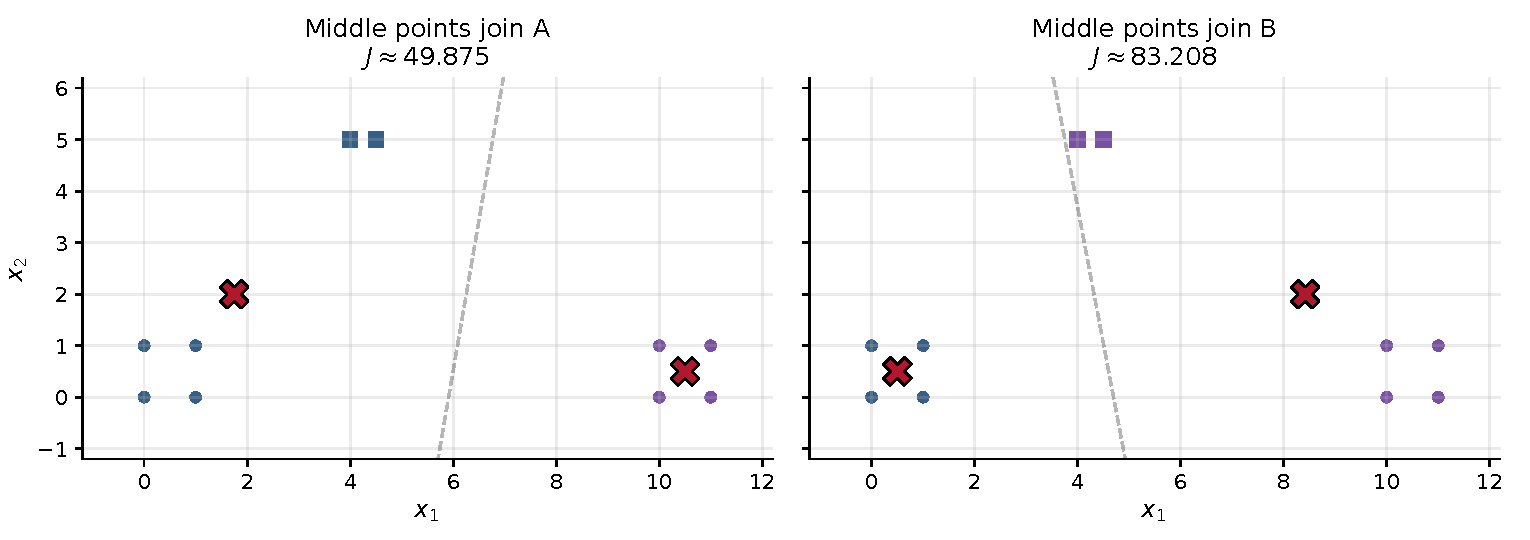
\includegraphics[width=\textwidth]{figures/handouts/em_algorithm/fig_kmeans_fixed_points}
  \caption{A toy $k$-means instance with two stable solutions depending on how the ambiguous ``middle'' points are assigned. Even in this simple setting, the update map has multiple basins and different fixed points can have different objective values.}
  \label{fig:kmeans-fixed-points}
\end{figure}

\Cref{fig:kmeans-fixed-points} makes the basin story visible.
The central points sit near an assignment boundary.
One initialization causes them to be claimed by the left cluster; another causes them to be claimed by the right cluster.
Once those assignments differ, the cluster means move differently, which reinforces the difference on the next E-step.
The stable solutions are therefore \emph{self-consistent latent assignments}.

This is exactly why initialization is part of the method rather than an afterthought.
In latent-variable problems one rarely hopes for a global theorem of the form ``EM converges to the best optimum from everywhere.''
Instead, the practical template is
\begin{algorithm}[H]
  \caption{Two-stage template: initialization + EM refinement}
  \label{alg:two-stage-em}
  \begin{algorithmic}[1]
    \Require Model class and EM operator $M_n$, plus a cheap initializer.
    \Ensure An estimate $\hat\theta$ intended to approximate a good population maximizer.
    \State \textbf{Initialization:} produce one or more candidates $\Theta_0$ (e.g.\ moments/spectral, $k$-means++, random restarts).
    \State Pick $\theta^{(0)}\in\Theta_0$ using a simple score (e.g.\ likelihood, held-out likelihood, or a surrogate).
    \State \textbf{Refinement:} run EM iterations $\theta^{(t+1)}=M_n(\theta^{(t)})$ until convergence; return the final iterate $\hat\theta$.
  \end{algorithmic}
\end{algorithm}

The Gaussian-mixture example later keeps the same logic but replaces hard assignments by soft responsibilities.
That makes the map smooth enough to analyze with derivatives, while preserving the same basin-versus-rate distinction.

\section[Gaussian mixture]{Example II: a two-component Gaussian mixture}
\label{sec:gmm-pop-em}

We now illustrate the contractive-map picture in the simplest EM setting: a balanced two-component Gaussian mixture with known variance.
To keep notation light, we work in one dimension and parameterize the unknown mean as $\theta^\star>0$; the model is
\[
Y \sim \tfrac12\,\mathcal{N}(\theta^\star,\sigma^2) + \tfrac12\,\mathcal{N}(-\theta^\star,\sigma^2),
\]
and we estimate $\theta\in\R$.
The latent variable is the component label.
This model makes the basin picture and the local-rate picture visible in the same calculation.
The same explicit map will explain why sign determines the basin and why separation controls the slope.

\subsection{EM operator and fixed points}
\label{subsec:gmm-em-operator}

Given a sample $\{y_i\}_{i=1}^n$, EM alternates between responsibilities
$w_\theta(y_i)=\Pr(Z=+1\mid Y=y_i,\theta)$ and maximizing the resulting quadratic surrogate $Q_n(\theta'\mid\theta)$.
In this model both steps have closed forms, so the update map is one-dimensional and explicit.

\subsubsection{Deriving the EM update in closed form}
\label{subsubsec:gmm-derivation}

We parameterize the mixture using a latent label $Z\in\{-1,+1\}$ with $\Pr(Z=+1)=\Pr(Z=-1)=1/2$ and
\[
Y\mid Z=z,\theta' \sim \mathcal{N}(z\theta',\sigma^2).
\]
The complete-data log-likelihood is (up to constants)
\[
\log f_{\theta'}(y,z) = -\frac{1}{2\sigma^2}\big(y-z\theta'\big)^2.
\]
By Bayes' rule, the responsibility is
\begin{align*}
w_\theta(y)
&=\Pr(Z=+1\mid Y=y,\theta)
=\frac{\exp\!\left(-\frac{(y-\theta)^2}{2\sigma^2}\right)}{\exp\!\left(-\frac{(y-\theta)^2}{2\sigma^2}\right)+\exp\!\left(-\frac{(y+\theta)^2}{2\sigma^2}\right)} \\
&=\frac{1}{1+\exp\!\left(-\frac{(y+\theta)^2-(y-\theta)^2}{2\sigma^2}\right)}
=\frac{1}{1+\exp\!\left(-\frac{2\theta y}{\sigma^2}\right)}.
\end{align*}
Here $(y+\theta)^2-(y-\theta)^2=4\theta y$, so the responsibility is a logistic function of $\theta y/\sigma^2$.
Equivalently,
\[
2w_\theta(y)-1 = \tanh\!\left(\frac{\theta y}{\sigma^2}\right),
\]
so the ``soft label'' $2w_\theta(y)-1$ is a smooth odd function of the score $\theta y$.

The sample $Q$-function is the conditional expectation of the complete-data log-likelihood,
\[
Q_n(\theta'\mid\theta)
=
-\frac{1}{2n\sigma^2}\sum_{i=1}^n\Big(
w_\theta(y_i)\,(y_i-\theta')^2 + (1-w_\theta(y_i))\,(y_i+\theta')^2
\Big),
\]
which is a concave quadratic function of $\theta'$.
Differentiate and set the derivative equal to $0$:
\[
0
=
\frac{\partial}{\partial \theta'}Q_n(\theta'\mid\theta)
=
\frac{1}{n\sigma^2}\sum_{i=1}^n\Big(
w_\theta(y_i)\,(y_i-\theta') - (1-w_\theta(y_i))\,(y_i+\theta')
\Big).
\]
Rearrange the term inside the sum as
\[
w_\theta(y_i)\,(y_i-\theta') - (1-w_\theta(y_i))\,(y_i+\theta')
=
\big(2w_\theta(y_i)-1\big)\,y_i-\theta',
\]
so the first-order condition becomes $0=\frac{1}{n\sigma^2}\sum_{i=1}^n\big(\big(2w_\theta(y_i)-1\big)\,y_i-\theta'\big)$.
Solving for $\theta'$ yields the closed-form M-step
\[
M_n(\theta)
=
\frac{1}{n}\sum_{i=1}^n \big(2w_\theta(y_i)-1\big)\,y_i
=
\frac{1}{n}\sum_{i=1}^n y_i\,\tanh\!\left(\frac{\theta y_i}{\sigma^2}\right).
\]
At the population level, the sample average is replaced by an expectation:
\[
M(\theta)
=
\E\!\left[\big(2w_\theta(Y)-1\big)\,Y\right]
=
\E\!\left[Y\,\tanh\!\left(\frac{\theta Y}{\sigma^2}\right)\right],
\]
yielding a deterministic update map $\theta^{t+1}=M(\theta^t)$.
This formula makes the geometry visible.
The score $\theta Y$ determines the posterior sign of the latent label, and the hyperbolic tangent turns that score into a soft label in $[-1,1]$.
When the mixture components are well separated, most draws of $Y$ make $\theta Y/\sigma^2$ large in magnitude, so the soft labels are close to $\pm 1$ and EM behaves almost like a hard assignment step.
When the components are weakly separated, the same soft labels stay closer to $0$, so the map lies nearer the diagonal and refinement is slower.

\begin{lemma}[Population fixed points for the symmetric mixture]
\label{lem:gmm-fixed-points}
Under the population model $Y=Z\theta^\star+\varepsilon$ with $Z\in\{-1,+1\}$ uniform and $\varepsilon\sim \mathcal{N}(0,\sigma^2)$ independent of $Z$, the population EM map satisfies
\[
M(\theta^\star)=\theta^\star,
\qquad
M(-\theta^\star)=-\theta^\star,
\qquad
M(0)=0.
\]
\end{lemma}

\begin{proof}
For any $\theta$, the posterior mean of the label is
\[
\E[Z\mid Y=y,\theta]
= (+1)\Pr(Z=+1\mid y,\theta) + (-1)\Pr(Z=-1\mid y,\theta)
=2w_\theta(y)-1.
\]
Therefore $M(\theta)=\E\!\left[Y\,\E[Z\mid Y,\theta]\right]$.
At $\theta=\theta^\star$, the conditional expectation is taken under the true model, so by the tower property
\[
M(\theta^\star)
=\E\!\left[Y\,\E[Z\mid Y,\theta^\star]\right]
=\E[YZ].
\]
Since $Y=Z\theta^\star+\varepsilon$ with $\varepsilon\perp Z$ and $Z^2=1$, we have $\E[YZ]=\E[(Z\theta^\star+\varepsilon)Z]=\theta^\star$.
The identity $M(-\theta^\star)=-\theta^\star$ follows by the same argument (or by symmetry of the model), and $M(0)=0$ follows because $w_0(y)=1/2$ so $2w_0(y)-1=0$.
\end{proof}

In this example the geometry assumption in \Cref{thm:em-fos-implies-contraction} is immediate:
the population objective $q(\theta')=Q(\theta'\mid\theta^\star)$ is a concave quadratic in $\theta'$ with second derivative $q''(\theta')=-1/\sigma^2$, hence it is globally $(1/\sigma^2)$-strongly concave.
The remaining step is to verify that the update map is stable in the basin of interest, which in one dimension reduces to controlling the slope $|M'(\theta)|$.

The third fixed point at $0$ plays a different role.
It is a self-consistent point in the sense that perfectly ambiguous responsibilities stay ambiguous, but it is not attractive.
The next exercise computes that instability directly.

\begin{exercise}[Instability of the zero fixed point in the Gaussian mixture map]
\label{ex:gmm-zero-unstable}
Consider the population EM map
\[
M(\theta)=\E\!\left[Y\,\tanh\!\left(\frac{\theta Y}{\sigma^2}\right)\right],
\qquad
Y=Z\theta^\star+\varepsilon,\ Z\in\{-1,+1\}\text{ uniform},\ \varepsilon\sim\mathcal{N}(0,\sigma^2).
\]
\begin{enumerate}[leftmargin=*]
  \item Show that $M$ is an odd function: $M(-\theta)=-M(\theta)$.
  \item Differentiate under the expectation to show
  \[
  M'(\theta)=\E\!\left[\frac{Y^2}{\sigma^2}\cdot \frac{1}{\cosh^2\!\left(\frac{\theta Y}{\sigma^2}\right)}\right].
  \]
  \item Compute $M'(0)$ and conclude that $0$ is a locally unstable fixed point (i.e.\ $|M'(0)|>1$).
\end{enumerate}
\end{exercise}

\SolutionBox[14]{%
\emph{Part (1).}
Using that $\tanh$ is odd,
\[
M(-\theta)
=\E\!\left[Y\,\tanh\!\left(-\frac{\theta Y}{\sigma^2}\right)\right]
=-\E\!\left[Y\,\tanh\!\left(\frac{\theta Y}{\sigma^2}\right)\right]
=-M(\theta).
\]

\emph{Part (2).}
Since $\frac{d}{du}\tanh(u)=\cosh^{-2}(u)$ and $\tanh,\cosh^{-2}$ are bounded, dominated convergence justifies differentiation under the expectation:
\[
M'(\theta)
=\E\!\left[Y\cdot \frac{Y}{\sigma^2}\cdot \frac{1}{\cosh^2\!\left(\frac{\theta Y}{\sigma^2}\right)}\right]
=\E\!\left[\frac{Y^2}{\sigma^2}\cdot \frac{1}{\cosh^2\!\left(\frac{\theta Y}{\sigma^2}\right)}\right].
\]

\emph{Part (3).}
At $\theta=0$, $\cosh^2(0)=1$, so $M'(0)=\E[Y^2]/\sigma^2$.
Under $Y=Z\theta^\star+\varepsilon$ with $Z^2=1$ and $\varepsilon\perp Z$,
\[
\E[Y^2]=\E[(Z\theta^\star+\varepsilon)^2]=(\theta^\star)^2+\sigma^2,
\]
so
\[
M'(0)=\frac{(\theta^\star)^2+\sigma^2}{\sigma^2}=1+\left(\frac{\theta^\star}{\sigma}\right)^2>1.
\]
Hence $0$ is a locally unstable fixed point.%
}

\Cref{fig:em-operator-fixed-points} now has a precise interpretation:
the graph shown there is exactly the map derived above.
The fixed points are its intersections with the diagonal.
Because the model is symmetric, the population log-likelihood has two equivalent maximizers $\pm\theta^\star$, and the sign of the initialization determines which one the iterates approach.
Here that nonconvexity is benign: the two limits differ only by label swapping, so they represent the same fitted mixture distribution.
Larger separation does not change the basin picture; it changes the rate of refinement within each basin.

\subsubsection{Global convergence of population EM in one dimension}
\label{subsubsec:gmm-global-population}

\Cref{fig:em-operator-fixed-points} suggests something stronger than local contraction near $\pm\theta^\star$: in one dimension, every initialization with the correct sign appears to converge to the corresponding population maximizer.
This is true, and it is a rare example where population EM admits a clean global guarantee.

To connect this claim with the literature, write the update map as a two-argument function.
For any $m>0$, let
\[
Y_m \sim \tfrac12\,\mathcal{N}(m,\sigma^2) + \tfrac12\,\mathcal{N}(-m,\sigma^2),
\qquad
M(\theta; m)\coloneqq \E\!\left[Y_m\,\tanh\!\left(\frac{\theta Y_m}{\sigma^2}\right)\right].
\]
Our population EM map is $\theta\mapsto M(\theta;\theta^\star)$, and (by the fixed point lemma) $M(m;m)=m$.

\begin{proposition}[Sign determines the basin in the 1D symmetric mixture]
\label{prop:gmm-global-population-sign-basin}
Assume $\theta^\star>0$.
Let $\theta^{(t+1)}=M(\theta^{(t)};\theta^\star)$ be the population EM iterates.
If $\theta^{(0)}>0$, then $\theta^{(t)}>0$ for all $t$ and $\theta^{(t)}\to \theta^\star$.
By symmetry, if $\theta^{(0)}<0$ then $\theta^{(t)}\to -\theta^\star$, and if $\theta^{(0)}=0$ then $\theta^{(t)}=0$ for all $t$.
\end{proposition}

\begin{proof}
If $\theta>0$, then $y\tanh(\theta y/\sigma^2)\ge 0$ for every $y$, with strict inequality for every $y\neq 0$.
Hence $M(\theta;\theta^\star)>0$, so positive initializations remain positive under the iteration.
The convergence claims are then exactly the one-dimensional specialization of \citet[Thms.~1--2]{xu_hsu_maleki_2016_global_em}: in one dimension, the sign condition $\ip{\theta^{(0)}}{\theta^\star}\gtrless 0$ reduces to $\theta^{(0)}\gtrless 0$, so the cited theorem says the population iterates converge to the corresponding signed maximizer, while the zero initialization remains at the unstable fixed point $0$.
\end{proof}

The same reference proves the higher-dimensional analogue, where the basin is determined by the sign of the inner product $\ip{\theta^{(0)}}{\theta^\star}$ rather than by the sign of a scalar initialization; see \citet[Thms.~1--2]{xu_hsu_maleki_2016_global_em}.

In one dimension, local contractivity near a fixed point is captured by the slope $|M'(\theta^\star)|$: smaller slope means faster refinement.
Since $M(\theta)=\E\!\left[Y\tanh\!\left(\frac{\theta Y}{\sigma^2}\right)\right]$ and $\frac{d}{du}\tanh(u)=\frac{1}{\cosh^2(u)}$, we can differentiate under the expectation to get
\[
M'(\theta)
=
\E\!\left[\frac{Y^2}{\sigma^2}\cdot \frac{1}{\cosh^2\!\left(\frac{\theta Y}{\sigma^2}\right)}\right].
\]
\Cref{fig:em-contraction-vs-snr} plots this slope as a function of the signal-to-noise ratio $\theta^\star/\sigma$ for the Gaussian mixture.
Separation plays the role of a \emph{conditioning parameter} for EM: when $\theta^\star/\sigma$ is large, responsibilities are close to $0$--$1$ under the true model and the map is strongly contractive, so refinement is fast; when $\theta^\star/\sigma$ is small, responsibilities stay near $1/2$ and the slope approaches $1$, so linear convergence becomes extremely slow.
Importantly, this ``slow EM'' regime is not a mysterious algorithmic failure---it reflects the fact that the statistical model itself becomes less distinctive as $\theta^\star/\sigma\to 0$:
the mixture distribution approaches a single Gaussian, so many parameter values yield almost the same observed-data likelihood and there is little signal for any method to exploit.
In other words, low separation is often ``easy'' in a \emph{model-fit} sense (many parameter values fit about equally well), but ``hard'' in a \emph{parameter-estimation} sense (it is difficult to reliably recover the tiny component separation).

\begin{lemma}[A simple sufficient condition for local contractivity]
\label{lem:gmm-contractive-region}
For any $\theta\neq 0$, the derivative satisfies
\[
0< M'(\theta) \le \frac{4e^{-2}\sigma^2}{\theta^2}.
\]
In particular, if $\theta^\star \ge \frac{4\sigma}{e}$, then $M$ is a contraction on the interval $\big[\frac{\theta^\star}{2},\frac{3\theta^\star}{2}\big]$ with contraction factor
\[
\kappa \le \frac{16e^{-2}\sigma^2}{(\theta^\star)^2} < 1.
\]
\end{lemma}

\clearpage
\begin{exercise}[Proving \Cref{lem:gmm-contractive-region}]
\label{ex:gmm-contractive-region}
Prove \Cref{lem:gmm-contractive-region}.
\emph{Hint:} start from $M'(\theta)=\E\!\left[\frac{Y^2}{\sigma^2}\cosh^{-2}\!\left(\frac{\theta Y}{\sigma^2}\right)\right]$,
use $\cosh(u)\ge \tfrac12 e^{|u|}$, and then maximize $y^2e^{-by}$ over $y\ge 0$ for $b>0$.
\end{exercise}

\SolutionBox[22]{%
Starting from
\[
M'(\theta)
=
\E\!\left[\frac{Y^2}{\sigma^2}\cdot \frac{1}{\cosh^2\!\left(\frac{\theta Y}{\sigma^2}\right)}\right],
\]
use $\cosh(u)\ge \tfrac12 e^{|u|}$ to obtain $\cosh^{-2}(u)\le 4e^{-2|u|}$.
Hence,
\[
M'(\theta)
\le
\frac{4}{\sigma^2}\E\!\left[Y^2\exp\!\left(-\frac{2|\theta|\,|Y|}{\sigma^2}\right)\right].
\]
Fix $b>0$.  For $y\ge 0$, the function $y\mapsto y^2e^{-by}$ has derivative $e^{-by}(2y-by^2)$, so it is maximized at $y=2/b$ with value $4e^{-2}/b^2$.
Therefore $Y^2e^{-b|Y|}\le 4e^{-2}/b^2$ almost surely, and with $b=\frac{2|\theta|}{\sigma^2}$ we get
\[
M'(\theta)
\le
\frac{4}{\sigma^2}\cdot \frac{4e^{-2}}{b^2}
=
\frac{4e^{-2}\sigma^2}{\theta^2}.
\]
If $\theta^\star\ge \frac{4\sigma}{e}$ and $\theta\in[\theta^\star/2,3\theta^\star/2]$, then $|\theta|\ge \theta^\star/2$ and the bound gives
\[
\sup_{\theta\in[\theta^\star/2,3\theta^\star/2]} M'(\theta)
\le
\frac{16e^{-2}\sigma^2}{(\theta^\star)^2}
<1,
\]
so $M$ is a contraction on this interval with contraction factor $\kappa\le 16e^{-2}\sigma^2/(\theta^\star)^2$.%
}

\begin{figure}[t]
  \centering
  \input{figures/handouts/em_algorithm/fig_em_contraction_vs_snr}
  \caption{Local contraction factor $|M'(\theta^\star)|$ for population EM in the symmetric two-component Gaussian mixture, as a function of the signal-to-noise ratio $\theta^\star/\sigma$. Larger separation leads to much stronger contractivity near the population maximizer, hence faster refinement once initialized in the correct basin.}
  \label{fig:em-contraction-vs-snr}
\end{figure}

\subsection{Local theory near a good fixed point}
\label{subsec:em-population-contractivity-template}

The Gaussian-mixture example already contains the shape of a general EM theorem.
Likelihood ascent is only part of the story.
It says that EM does not decrease the observed-data likelihood, but it does not say whether the initialization lies in the basin of a desirable fixed point, whether the population map pulls the iterates back once they are near that point, or whether finite-sample noise distorts that picture.
That is why useful EM results are usually local.

To study the local behavior near a good population fixed point $\theta^\star$, freeze the second argument of the surrogate at $\theta^\star$ and define
\[
q(\theta') \coloneqq Q(\theta' \mid \theta^\star).
\]
This is the surrogate EM would maximize if the E-step already used the correct posterior law.
From that viewpoint, the local theory is built out of two ideas.
First, the ideal objective $q$ should have enough curvature near $\theta^\star$ that maximizing it would correct small perturbations away from the target.
Second, the E-step should be stable: replacing $\theta^\star$ by a nearby iterate $\theta$ should not change the surrogate gradient too much.
If both statements hold, then the true EM map behaves like a perturbed maximization of $q$, so one can prove contraction for the population map and then transfer that result to the sample map by a perturbation argument.
The next definitions write those two ideas in a form suitable for the proof.

\begin{definition}[Local strong concavity]
\label{def:em-local-strong-concavity}
Fix $r>0$ and define the ball $B_r(\theta^\star)\coloneqq\{\theta\in\Theta:\norm{\theta-\theta^\star}_2\le r\}$.
We say $q$ is \textbf{$\lambda$-strongly concave on $B_r(\theta^\star)$} if for all $\theta_1,\theta_2\in B_r(\theta^\star)$,
\[
q(\theta_1)
\le
q(\theta_2)
\;+\;
\ip{\nabla q(\theta_2)}{\theta_1-\theta_2}
\;-\;
\frac{\lambda}{2}\norm{\theta_1-\theta_2}_2^2.
\]
\end{definition}

\begin{definition}[First-order stability (FOS)]
\label{def:em-fos}
Fix $r>0$.
We say the population $Q$-functions satisfy \textbf{$\mathrm{FOS}(\gamma)$ on $B_r(\theta^\star)$} if for all $\theta\in B_r(\theta^\star)$,
\[
\norm{\nabla_{\theta'} Q(M(\theta)\mid \theta^\star)-\nabla_{\theta'} Q(M(\theta)\mid \theta)}_2
\le
\gamma \norm{\theta-\theta^\star}_2.
\]
\end{definition}

\begin{theorem}[FOS + strong concavity $\Rightarrow$ contraction of population EM]
\label{thm:em-fos-implies-contraction}
Fix $r>0$ and define $B_r(\theta^\star)$ as in \Cref{def:em-local-strong-concavity}.
Assume:
\begin{enumerate}[leftmargin=*]
  \item $\theta^\star$ is self-consistent, meaning $M(\theta^\star)=\theta^\star$.
  \item $q(\cdot)=Q(\cdot\mid\theta^\star)$ is $\lambda$-strongly concave on $B_r(\theta^\star)$.
  \item $\mathrm{FOS}(\gamma)$ holds on $B_r(\theta^\star)$ for some $\gamma\in[0,\lambda)$.
  \item For all $\theta\in B_r(\theta^\star)$, the update $M(\theta)$ also lies in $B_r(\theta^\star)$.
  \item $\theta^\star$ is an interior maximizer of $q$, and for each $\theta\in B_r(\theta^\star)$ the EM update $M(\theta)$ is an interior maximizer of $\theta'\mapsto Q(\theta'\mid\theta)$, so that
  \[
  \nabla q(\theta^\star)=0,
  \qquad
  \nabla_{\theta'} Q(M(\theta)\mid\theta)=0.
  \]
\end{enumerate}
Then $M$ is contractive on $B_r(\theta^\star)$ with contraction factor $\kappa=\gamma/\lambda$:
\[
\norm{M(\theta)-\theta^\star}_2
\le
\frac{\gamma}{\lambda}\norm{\theta-\theta^\star}_2
\qquad\text{for all }\theta\in B_r(\theta^\star).
\]
\end{theorem}

\begin{proof}
Fix $\theta\in B_r(\theta^\star)$ and write $\bar\theta \coloneqq M(\theta)$.
By local invariance, $\bar\theta\in B_r(\theta^\star)$.
By \Cref{def:em-local-strong-concavity}, the function $-q$ is $\lambda$-strongly convex on $B_r(\theta^\star)$, so for all $u,v\in B_r(\theta^\star)$,
\[
\ip{\nabla q(u)-\nabla q(v)}{u-v}
\le
-\lambda\norm{u-v}_2^2,
\]
and therefore, by Cauchy--Schwarz,
\[
\lambda\norm{u-v}_2
\le
\norm{\nabla q(u)-\nabla q(v)}_2.
\]
Apply this with $u=\bar\theta$ and $v=\theta^\star$, and use $\nabla q(\theta^\star)=0$, to obtain
\[
\lambda\norm{\bar\theta-\theta^\star}_2
\le
\norm{\nabla q(\bar\theta)}_2
=
\norm{\nabla_{\theta'} Q(\bar\theta\mid\theta^\star)}_2.
\]
By the interior optimality condition $\nabla_{\theta'} Q(\bar\theta\mid\theta)=0$ and $\mathrm{FOS}(\gamma)$,
\[
\norm{\nabla_{\theta'} Q(\bar\theta\mid\theta^\star)}_2
=
\norm{\nabla_{\theta'} Q(\bar\theta\mid\theta^\star)-\nabla_{\theta'} Q(\bar\theta\mid\theta)}_2
\le
\gamma\norm{\theta-\theta^\star}_2.
\]
Combine the last two displays and divide by $\lambda$.
\end{proof}

In words, strong concavity tells us that the ideal M-step would correct deviations from $\theta^\star$, while FOS says the real E-step does not distort that ideal picture too much.
If FOS fails badly, then changing the current iterate can change the posterior weights so much that the update map loses its restorative pull.

\subsubsection{Gradient EM: an inexact M-step}
\label{subsec:em-gradient-em}

In large models, the exact maximization step defining $M(\theta)$ can be expensive.
A common alternative is to take one gradient ascent step on the surrogate $Q(\cdot\mid\theta)$ starting from $\theta$.
At the population level, this defines the \emph{gradient EM} operator
\[
G(\theta)\coloneqq \theta + \alpha\,\nabla_{\theta'} Q(\theta\mid\theta),
\]
where $\alpha>0$ is a step size.
(The sample version replaces $Q$ by $Q_n$.)

If we could take gradient ascent on the ideal objective $q(\theta)=Q(\theta\mid\theta^\star)$ directly, then strong concavity and smoothness would give a contraction for an appropriate step size; see \citep[\S9.2]{boyd_vandenberghe_2004_convex}.
Gradient EM behaves similarly when the surrogate gradient is stable near $\theta^\star$.

\begin{definition}[Gradient stability (GS)]
\label{def:em-gs}
Fix $r>0$.
We say the population $Q$-functions satisfy \textbf{$\mathrm{GS}(\gamma)$ on $B_r(\theta^\star)$} if for all $\theta\in B_r(\theta^\star)$,
\[
\norm{\nabla_{\theta'} Q(\theta\mid \theta^\star)-\nabla_{\theta'} Q(\theta\mid \theta)}_2
\le
\gamma \norm{\theta-\theta^\star}_2.
\]
\end{definition}

\begin{theorem}[GS + strong concavity $\Rightarrow$ contraction of gradient EM]
\label{thm:em-gs-implies-contraction}
Fix $r>0$ and assume:
\begin{enumerate}[leftmargin=*]
  \item $q(\cdot)=Q(\cdot\mid\theta^\star)$ is $\lambda$-strongly concave and $L$-smooth on $B_r(\theta^\star)$, with $0<\lambda\le L$.
  \item $\mathrm{GS}(\gamma)$ holds on $B_r(\theta^\star)$ for some $\gamma\in[0,\lambda)$.
  \item $\theta^\star$ is an interior maximizer of $q$, so $\nabla q(\theta^\star)=0$.
\end{enumerate}
Then gradient EM with step size $\alpha=\frac{2}{L+\lambda}$ is contractive on $B_r(\theta^\star)$:
\[
\norm{G(\theta)-\theta^\star}_2
\le
\left(\frac{L-\lambda+2\gamma}{L+\lambda}\right)\norm{\theta-\theta^\star}_2
\qquad\text{for all }\theta\in B_r(\theta^\star).
\]
\end{theorem}

\begin{proof}
Write $G(\theta)-\theta^\star$ as
\[
\underbrace{\theta + \alpha \nabla q(\theta)-\theta^\star}_{\text{gradient ascent on $q$}}
\;+\;
\alpha\underbrace{\bigl(\nabla_{\theta'} Q(\theta\mid\theta)-\nabla_{\theta'} Q(\theta\mid\theta^\star)\bigr)}_{\text{stability error}}.
\]
For $\alpha=\frac{2}{L+\lambda}$, gradient ascent on a $\lambda$-strongly concave, $L$-smooth function is a contraction mapping with factor $\frac{L-\lambda}{L+\lambda}$ (equivalently, apply the standard strongly convex result to $-q$).
Combine this with \Cref{def:em-gs} and $\alpha=\frac{2}{L+\lambda}$ to get
\[
\norm{G(\theta)-\theta^\star}_2
\le
\left(\frac{L-\lambda}{L+\lambda} + \frac{2\gamma}{L+\lambda}\right)\norm{\theta-\theta^\star}_2,
\]
which is the claim.
\end{proof}

Once a population contraction factor is available for either exact EM or gradient EM, the sample-level picture follows from a perturbation argument.

\begin{lemma}[Contraction + perturbation $\Rightarrow$ convergence to a neighborhood]
\label{lem:contraction-perturbation}
Fix a point $\theta^\star\in\Theta$ and a radius $r>0$.
Assume:
\begin{enumerate}[leftmargin=*]
  \item $M(\theta^\star)=\theta^\star$ and, for all $\theta$ with $\norm{\theta-\theta^\star}_2\le r$,
  \[
  \norm{M(\theta)-\theta^\star}_2 \le \kappa \norm{\theta-\theta^\star}_2
  \quad\text{for some }\kappa\in(0,1).
  \]
  \item For all $\theta$ with $\norm{\theta-\theta^\star}_2\le r$,
  \[
  \norm{M_n(\theta)-M(\theta)}_2 \le \varepsilon_n.
  \]
\end{enumerate}
Then any iterate sequence $\theta^{t+1}=M_n(\theta^t)$ that remains in the ball satisfies
\[
\norm{\theta^t-\theta^\star}_2
\le
\kappa^t \norm{\theta^0-\theta^\star}_2 + \frac{\varepsilon_n}{1-\kappa}.
\]
\end{lemma}

\begin{proof}
Write
\[
\norm{\theta^{t+1}-\theta^\star}_2
\le
\norm{M(\theta^t)-\theta^\star}_2 + \norm{M_n(\theta^t)-M(\theta^t)}_2
\le
\kappa\norm{\theta^t-\theta^\star}_2 + \varepsilon_n,
\]
then unroll the recursion.
\end{proof}

\Cref{lem:contraction-perturbation} is the core population-to-sample message.
Inside a basin where the sample map stays uniformly close to the population map, optimization error decays geometrically until it reaches a floor of order $\varepsilon_n/(1-\kappa)$.
Equivalently, sample EM converges to the sample fixed point in its basin, while the gap between that sample target and the population target is the residual statistical error.

\subsection{Finite-sample EM: geometric decay until a floor}
\label{sec:finite-sample-floor}

At finite $n$, the operator $M_n$ fluctuates around $M$.
In a neighborhood where $M$ is contractive and $M_n$ is uniformly close to $M$, \Cref{lem:contraction-perturbation} gives geometric decay until the remaining error is on the order of $1/\sqrt{n}$.

\begin{figure}[t]
  \centering
  \input{figures/handouts/em_algorithm/fig_em_population_vs_sample_convergence}
  \caption{Distance to $\theta^\star$ versus EM iteration in the Gaussian mixture example. Population EM converges linearly to $\theta^\star$. Sample EM tracks the population dynamics until it reaches a sample-dependent floor.}
  \label{fig:em-pop-vs-sample}
\end{figure}

In this example, once the initialization lands in the correct basin, the population map is contractive and the sample map tracks it until the iterate reaches an $n$-dependent statistical floor.
Separation does not change which basin is correct; it changes the speed of refinement inside that basin.

A systematic development of this population-to-sample contraction argument appears in \citet[Thm.~1]{balakrishnan_wainwright_yu_2014_em}.
Moreover, this two-Gaussian mixture is one of the rare latent-variable models where much stronger \emph{global} guarantees are possible; see, e.g., \citet[Thm.~1]{xu_hsu_maleki_2016_global_em}.

\clearpage
% ------------------------------------------------------------
\section[Missing covariates]{Example III: regression with missing covariates}
\label{sec:missing-covariates}

EM is also natural outside mixture models whenever part of the data is latent or unobserved.
A basic example is linear regression with covariates missing completely at random.
Let $X\in\R^d$ and $Y\in\R$ follow the population model
\[
X \sim \mathcal{N}(0,I_d),
\qquad
Y = \ip{X}{\theta^\star} + \varepsilon,
\qquad
\varepsilon \sim \mathcal{N}(0,\sigma^2)\ \text{independent of }X,
\]
and suppose we observe $Y$ but only a subset of the coordinates of $X$.
Formally, each coordinate is missing with probability $\rho\in[0,1)$, independently across coordinates and samples.
The missing coordinates are treated as latent variables, so EM alternates between imputing them from the conditional law of $X$ given $(X_{\mathrm{obs}},Y)$ and refitting $\theta'$ by weighted least squares using the conditional moments $\E[X\mid X_{\mathrm{obs}},Y,\theta]$ and $\E[XX^\top\mid X_{\mathrm{obs}},Y,\theta]$.

This example complements the Gaussian mixture.
In the mixture model, weak separation mainly makes the EM map flatter near the correct target.
Here the more basic issue is that the E-step literally fills in unseen coordinates using the \emph{current} parameter.
If $\theta$ is already close to $\theta^\star$, those imputations are helpful.
If $\theta$ points in a badly wrong direction and the missingness level is high, the imputations can reinforce that wrong direction, so the map itself can develop a bad stable fixed point.

\subsection{Missingness and identifiability}
\label{subsec:missing-covariates-identifiability-limit}

As $\rho$ increases, fewer coordinates of $X$ are observed, the E-step becomes less informative, and both optimization and statistical estimation become harder.

The extreme case $\rho=1$ shows the identifiability issue most clearly.
If all covariates are missing, then the observed data are only the responses $\{Y_i\}_{i=1}^n$.
Because $X\sim\mathcal{N}(0,I_d)$, for any parameter $\theta$ we have $\ip{X}{\theta}\sim \mathcal{N}(0,\norm{\theta}_2^2)$, so
\[
Y \mid \theta
\sim
\mathcal{N}\!\big(0,\norm{\theta}_2^2+\sigma^2\big).
\]
Therefore the distribution of the observed data depends on $\theta$ only through $\norm{\theta}_2$.
In particular, the direction of $\theta^\star$ is \emph{not identifiable}: any $\tilde\theta$ with $\norm{\tilde\theta}_2=\norm{\theta^\star}_2$ produces the same law for $Y$.
No algorithm (EM included) can recover what the data do not contain; at best, one can hope to estimate $\norm{\theta^\star}_2$.
\Cref{fig:em-nonidentifiability-ridge} gives a schematic picture.

\begin{figure}[t]
  \centering
  \input{figures/handouts/em_algorithm/fig_em_nonidentifiability_ridge}
  \caption{Non-identifiability in the ``noise-only'' limit.  When $\rho=1$, we never observe any coordinates of $X$, and the marginal law is $Y\mid\theta\sim\mathcal{N}(0,\norm{\theta}_2^2+\sigma^2)$.  Hence all parameters on a sphere $\{\theta:\norm{\theta}_2=\text{const}\}$ induce the same distribution of $Y$, so there cannot be a contraction toward a unique maximizer.}
  \label{fig:em-nonidentifiability-ridge}
\end{figure}

This illustrates a different failure mode than low separation in mixtures.
In Example II, low separation mainly means weak identification and poor conditioning: there is a well-defined population target up to the sign symmetry, but the likelihood is relatively flat and the EM contraction factor is close to $1$, so refinement is slow and statistical accuracy requires very large $n$.
Here, increasing missingness pushes the statistical problem itself toward non-identifiability, so EM no longer has a unique population target to contract toward.

\subsection{Deriving the EM operator in closed form}
\label{subsec:missing-covariates-derivation}

Because the model is Gaussian, the E-step conditional moments can be written explicitly and the M-step reduces to a linear system.
These formulas show exactly where the self-reinforcement enters:
the posterior moments used in the E-step depend on the current iterate $\theta$, so the regression problem solved by the M-step is built out of \emph{imputed} covariates that already reflect the current belief.

\subsubsection{E-step: conditional moments from a joint Gaussian}
\label{subsubsec:missing-covariates-estep}

Fix one observation $(x_{\mathrm{obs}},y)$ and let $O\subseteq\{1,\dots,d\}$ be the set of observed coordinates, with $M$ its complement.
Write the parameter and covariate vector in blocks $\theta=(\theta_M,\theta_O)$ and $X=(X_M,X_O)$.
Conditioned on $X_O=x_O$, the scalar response model under parameter $\theta$ is
\[
Y = \ip{\theta_O}{x_O} + \ip{\theta_M}{X_M} + \varepsilon,
\qquad
X_M\sim\mathcal{N}(0,I),
\qquad
\varepsilon\sim\mathcal{N}(0,\sigma^2),
\]
so $X_M\mid (X_O=x_O,Y=y,\theta)$ is the Gaussian posterior in a one-dimensional linear measurement model.
A standard conditioning calculation (e.g.\ via Sherman--Morrison) yields
\begin{align}
\label{eq:missing-covariates-posterior-mean}
\E[X_M\mid x_O,y,\theta]
&=
\frac{\theta_M}{\sigma^2+\norm{\theta_M}_2^2}\,\Big(y-\ip{\theta_O}{x_O}\Big), \\
\label{eq:missing-covariates-posterior-cov}
\mathrm{Cov}(X_M\mid x_O,y,\theta)
&=
I-\frac{\theta_M\theta_M^\top}{\sigma^2+\norm{\theta_M}_2^2}.
\end{align}

Define the conditional mean and second moment of the \emph{full} covariate vector,
\[
\mu_\theta(x_{\mathrm{obs}},y)\coloneqq \E[X\mid X_{\mathrm{obs}}=x_{\mathrm{obs}},Y=y,\theta],
\qquad
\Sigma_\theta(x_{\mathrm{obs}},y)\coloneqq \E[XX^\top\mid X_{\mathrm{obs}}=x_{\mathrm{obs}},Y=y,\theta].
\]
Then $\mu_\theta$ agrees with the observed coordinates and uses \eqref{eq:missing-covariates-posterior-mean} for the missing coordinates:
\[
(\mu_\theta)_O = x_O,
\qquad
(\mu_\theta)_M = \E[X_M\mid x_O,y,\theta].
\]
Similarly, $\Sigma_\theta$ is obtained by combining the posterior covariance \eqref{eq:missing-covariates-posterior-cov} with the rank-one term from the posterior mean:
\[
(\Sigma_\theta)_{MM}
=
\mathrm{Cov}(X_M\mid x_O,y,\theta) + \E[X_M\mid x_O,y,\theta]\E[X_M\mid x_O,y,\theta]^\top,
\qquad
(\Sigma_\theta)_{OO}=x_Ox_O^\top,
\]
and the cross moments satisfy $(\Sigma_\theta)_{MO}=\E[X_M\mid x_O,y,\theta]\,x_O^\top$ and $(\Sigma_\theta)_{OM}=x_O\,\E[X_M\mid x_O,y,\theta]^\top$.

\clearpage
This Gaussian-conditioning algebra is the exact E-step calculation underlying the formulas above.
\begin{exercise}[Deriving the E-step conditional moments in the missing-covariates model]
\label{ex:missing-covariates-estep}
In \Cref{subsubsec:missing-covariates-estep}, fix a set of observed coordinates $O$ with complement $M$, and fix one observation $(x_O,y)$.
Consider the linear-Gaussian model
\[
X_M\sim\mathcal{N}(0,I),
\qquad
Y=\ip{\theta_O}{x_O}+\ip{\theta_M}{X_M}+\varepsilon,
\qquad
\varepsilon\sim\mathcal{N}(0,\sigma^2)\ \text{independent of }X_M.
\]
Show that the posterior is Gaussian with mean and covariance
\[
\E[X_M\mid x_O,y,\theta]=\frac{\theta_M}{\sigma^2+\norm{\theta_M}_2^2}\,\Big(y-\ip{\theta_O}{x_O}\Big),
\qquad
\mathrm{Cov}(X_M\mid x_O,y,\theta)=I-\frac{\theta_M\theta_M^\top}{\sigma^2+\norm{\theta_M}_2^2}.
\]
\emph{Hint:} write $(X_M,\;Y-\ip{\theta_O}{x_O})$ as a jointly Gaussian pair and use the standard conditional Gaussian formula.
\end{exercise}

\SolutionBox[18]{%
This is the standard conditional-Gaussian calculation behind the E-step.
Define the centered scalar $\tilde Y\coloneqq Y-\ip{\theta_O}{x_O}=\ip{\theta_M}{X_M}+\varepsilon$.
Then $(X_M,\tilde Y)$ is jointly Gaussian with
\[
\E[X_M]=0,
\qquad
\E[\tilde Y]=0,
\qquad
\mathrm{Cov}(X_M)=I.
\]
Moreover,
\[
\mathrm{Cov}(X_M,\tilde Y)
=
\E[X_M(\theta_M^\top X_M+\varepsilon)]
=
\E[X_M X_M^\top]\theta_M
=\theta_M,
\]
and
\[
\mathrm{Var}(\tilde Y)
=
\mathrm{Var}(\theta_M^\top X_M)+\mathrm{Var}(\varepsilon)
=
\norm{\theta_M}_2^2+\sigma^2.
\]
For a jointly Gaussian pair $(U,V)$ with $\mathrm{Var}(V)>0$, the conditional law is
\[
U\mid(V=v)\sim \mathcal{N}\!\left(\mathrm{Cov}(U,V)\,\mathrm{Var}(V)^{-1}v,\;\mathrm{Cov}(U)-\mathrm{Cov}(U,V)\,\mathrm{Var}(V)^{-1}\mathrm{Cov}(V,U)\right).
\]
Apply this with $U=X_M$ and $V=\tilde Y$ to obtain
\[
\E[X_M\mid \tilde Y=\tilde y]=\frac{\theta_M}{\sigma^2+\norm{\theta_M}_2^2}\,\tilde y,
\qquad
\mathrm{Cov}(X_M\mid \tilde Y)=I-\frac{\theta_M\theta_M^\top}{\sigma^2+\norm{\theta_M}_2^2}.
\]
Substitute $\tilde y=y-\ip{\theta_O}{x_O}$ to match \eqref{eq:missing-covariates-posterior-mean}--\eqref{eq:missing-covariates-posterior-cov}.%
}
\subsubsection{M-step: a quadratic \texorpdfstring{$Q_n$}{Qn} and a linear system}
\label{subsubsec:missing-covariates-mstep}

The complete-data log-likelihood for a single pair $(x,y)$ is
\[
\log f_{\theta'}(x,y)
=
C
-\frac{1}{2}\norm{x}_2^2
-\frac{1}{2\sigma^2}\big(y-\ip{x}{\theta'}\big)^2.
\]
In the $Q$-function, we take the conditional expectation over the missing covariates under the current iterate $\theta$.
The term $\norm{x}_2^2$ does not depend on $\theta'$, and the factor $1/\sigma^2$ does not affect the argmax, so it is enough to expand the expected squared error.
For one observation,
\begin{align*}
\E\Big[\big(y-\ip{X}{\theta'}\big)^2\mid x_{\mathrm{obs}},y,\theta\Big]
&=
y^2 - 2y\,\ip{\E[X\mid x_{\mathrm{obs}},y,\theta]}{\theta'}
  + \E\big[\theta'^\top XX^\top \theta'\mid x_{\mathrm{obs}},y,\theta\big] \\
&=
y^2 - 2y\,\ip{\mu_\theta(x_{\mathrm{obs}},y)}{\theta'}
  + \theta'^\top \Sigma_\theta(x_{\mathrm{obs}},y)\,\theta'.
\end{align*}
Summing over samples, and dropping additive constants that do not affect the maximizer, yields the quadratic form
\[
Q_n(\theta'\mid\theta)
=
-\frac{1}{2n}\sum_{i=1}^n
\Big(\theta'^\top \Sigma_\theta(x_{\mathrm{obs},i},y_i)\,\theta'
-2y_i\,\ip{\mu_\theta(x_{\mathrm{obs},i},y_i)}{\theta'}\Big).
\]
Taking a gradient in $\theta'$ and setting it equal to zero gives a linear system for the M-step:
\[
\left(\frac{1}{n}\sum_{i=1}^n \Sigma_\theta(x_{\mathrm{obs},i},y_i)\right)\theta'
=
\frac{1}{n}\sum_{i=1}^n y_i\,\mu_\theta(x_{\mathrm{obs},i},y_i),
\]
so, whenever the averaged conditional second-moment matrix is invertible, the unique sample M-step is
\[
M_n(\theta)
=
\left(\frac{1}{n}\sum_{i=1}^n \Sigma_\theta(x_{\mathrm{obs},i},y_i)\right)^{-1}
\left(\frac{1}{n}\sum_{i=1}^n y_i\,\mu_\theta(x_{\mathrm{obs},i},y_i)\right).
\]
The population operator $M$ has the same form with empirical averages replaced by expectations, again when the corresponding population matrix is nonsingular.
Here the relationship between $M$ and $M_n$ is direct: $M_n$ is the perturbation produced by replacing expectations with sample averages.

As a useful check, if there is no missingness ($\rho=0$), then $\mu_\theta(x_{\mathrm{obs}},y)=x$ and $\Sigma_\theta(x_{\mathrm{obs}},y)=xx^\top$ regardless of $\theta$, so $M_n(\theta)$ reduces to ordinary least squares and does not depend on the current iterate.

\subsubsection{A one-dimensional verification: explicit population map and local slope}
\label{subsubsec:missing-covariates-1d-check}

The full verification of contractivity for the missing-covariates model is algebraically involved in general dimension.
In one dimension the population EM map has a closed form, so the stability calculation can be carried out directly.
As in the Gaussian mixture, the population objective $q(\theta')=Q(\theta'\mid\theta^\star)$ is a concave quadratic in $\theta'$ with Hessian $-\sigma^{-2}I$, so the main issue is not the local geometry of $q$ but the stability of the E-step as $\theta$ varies.

Assume $d=1$.
Each sample either reveals $X$ (with probability $1-\rho$) or hides it (with probability $\rho$), and we always observe $Y=\theta^\star X+\varepsilon$.
When $X$ is missing, the E-step uses the Gaussian posterior under the current iterate $\theta$:
\[
X\mid (Y=y,\theta) \sim \mathcal{N}\!\left(\frac{\theta}{\theta^2+\sigma^2}y,\;\frac{\sigma^2}{\theta^2+\sigma^2}\right),
\]
so
\[
\mu_\theta(y) \coloneqq \E[X\mid Y=y,\theta] = \frac{\theta}{\theta^2+\sigma^2}y,
\qquad
\Sigma_\theta(y) \coloneqq \E[X^2\mid Y=y,\theta]
=
\frac{\sigma^2}{\theta^2+\sigma^2}+\mu_\theta(y)^2.
\]
When $X$ is observed, we simply have $\mu_\theta(x,y)=x$ and $\Sigma_\theta(x,y)=x^2$.

At the population level, the M-step takes the same linear-system form as above, which in one dimension simplifies to
\[
M(\theta)
=
\frac{\E\!\left[Y\,\mu_\theta(X_{\mathrm{obs}},Y)\right]}{\E\!\left[\Sigma_\theta(X_{\mathrm{obs}},Y)\right]}.
\]
Using the missingness decomposition and the identities
$\E[YX]=\theta^\star$, $\E[X^2]=1$, and $\E[Y^2]=(\theta^\star)^2+\sigma^2$, we obtain
\begin{align}
\label{eq:missing-covariates-1d-pop-map}
M(\theta)
&=
\frac{(1-\rho)\,\theta^\star
\;+\;\rho\,\frac{\theta}{\theta^2+\sigma^2}\big((\theta^\star)^2+\sigma^2\big)}
{(1-\rho)\cdot 1
\;+\;\rho\left(\frac{\sigma^2}{\theta^2+\sigma^2}
\;+\;\frac{\theta^2}{(\theta^2+\sigma^2)^2}\big((\theta^\star)^2+\sigma^2\big)\right)}.
\end{align}
Plugging in $\theta=\theta^\star$ gives $M(\theta^\star)=\theta^\star$ (the numerator becomes $\theta^\star$ and the denominator becomes $1$).

The structure of \eqref{eq:missing-covariates-1d-pop-map} is revealing.
The fully observed fraction $(1-\rho)$ contributes a direct pull toward $\theta^\star$.
The missing fraction $\rho$ contributes a term proportional to
\[
\frac{\theta}{\theta^2+\sigma^2},
\]
which depends on the \emph{current iterate}.
That is the self-reinforcing part of EM in this model:
when a covariate is unobserved, the E-step replaces it by a conditional mean whose sign and magnitude are already filtered through $\theta$.
At small $\rho$ the observed-data pull dominates.
At large $\rho$, the feedback through the current iterate can become strong enough to create additional fixed points.

We can also differentiate \eqref{eq:missing-covariates-1d-pop-map} to quantify the local contraction factor.
Write $M(\theta)=N(\theta)/D(\theta)$, where
\[
N(\theta) \coloneqq (1-\rho)\,\theta^\star + \rho\,\frac{\theta}{\theta^2+\sigma^2}\big((\theta^\star)^2+\sigma^2\big),
\]
and
\[
D(\theta)\coloneqq (1-\rho)+\rho\left(\frac{\sigma^2}{\theta^2+\sigma^2}
+\frac{\theta^2}{(\theta^2+\sigma^2)^2}\big((\theta^\star)^2+\sigma^2\big)\right).
\]
Then $N(\theta^\star)=\theta^\star$ and $D(\theta^\star)=1$.
Differentiate:
\[
N'(\theta)
=
\rho\big((\theta^\star)^2+\sigma^2\big)\cdot \frac{\sigma^2-\theta^2}{(\theta^2+\sigma^2)^2},
\]
and
\[
D'(\theta)
=
\rho\left(
-\frac{2\sigma^2\theta}{(\theta^2+\sigma^2)^2}
+2\big((\theta^\star)^2+\sigma^2\big)\cdot \frac{\theta(\sigma^2-\theta^2)}{(\theta^2+\sigma^2)^3}
\right).
\]
Evaluating at $\theta=\theta^\star$ and using the quotient rule gives
\[
M'(\theta^\star)
=
\frac{N'(\theta^\star)D(\theta^\star)-N(\theta^\star)D'(\theta^\star)}{D(\theta^\star)^2}
=
N'(\theta^\star)-\theta^\star D'(\theta^\star)
=
\rho\,\frac{(\theta^\star)^4+\sigma^4}{\big((\theta^\star)^2+\sigma^2\big)^2}.
\]
In particular, since $(\theta^\star)^4+\sigma^4 \le \big((\theta^\star)^2+\sigma^2\big)^2$, we have $0<M'(\theta^\star)\le \rho$.
In this simplest case, the local contraction factor worsens roughly linearly with the missingness probability $\rho$.
It equals $0$ when $\rho=0$, reflecting the fact that in the fully observed model the population M-step jumps to $\theta^\star$ in one iteration.

\subsubsection{A sharp counterexample: a spurious stable fixed point at high missingness}
\label{subsubsec:missing-covariates-spurious-fixed-point}

The local-slope calculation above can make it seem as if missingness only slows EM down.
However, even in one dimension (where the model is identifiable for every $\rho<1$), the population EM map can have \emph{multiple} stable fixed points when $\rho$ is large.
This is a genuinely nonconvex phenomenon: it is present even at the population level, so it cannot be blamed on finite-sample noise.

To see this explicitly, fix $\theta^\star=1$ and $\sigma=1$.
For $\rho=0.95$, the closed-form population map \eqref{eq:missing-covariates-1d-pop-map} becomes a rational function $M(\theta)$.
Define $f(\theta)\coloneqq M(\theta)-\theta$.

\clearpage
\begin{exercise}[A spurious fixed point from high missingness (1D)]
\label{ex:missing-covariates-spurious-fixed-point}
In the one-dimensional setting with $\theta^\star=\sigma=1$ and $\rho=0.95$, consider the population map \eqref{eq:missing-covariates-1d-pop-map} and define $f(\theta)=M(\theta)-\theta$.
\begin{enumerate}[leftmargin=*]
  \item Compute $f(-1)$ and $f(-0.5)$, and use the intermediate value theorem to show that $M$ has a fixed point in $(-1,-0.5)$.
  \item Compute $f(-0.1)$ and $f(0)$, and show that $M$ has a fixed point in $(-0.1,0)$.
  \item Explain why this implies that the population map has at least three fixed points for this parameter choice.
\end{enumerate}
\end{exercise}

\SolutionBox[22]{%
We use the closed form \eqref{eq:missing-covariates-1d-pop-map} with $\theta^\star=\sigma=1$ and $\rho=0.95$.

\emph{Part (1).}
For $\theta=-1$, note that $\theta^2+\sigma^2=2$ and $(\theta^\star)^2+\sigma^2=2$, so the numerator is
\[
(1-\rho)\theta^\star+\rho\,\frac{\theta}{\theta^2+\sigma^2}\big((\theta^\star)^2+\sigma^2\big)
=0.05\cdot 1+0.95\cdot\frac{-1}{2}\cdot 2
=-0.9,
\]
and the denominator is $0.05+0.95\cdot(1/2+1/2)=1$.
Thus $M(-1)=-0.9$ and $f(-1)=M(-1)-(-1)=0.1>0$.

For $\theta=-0.5$, we have $\theta^2+\sigma^2=1.25$ and $(\theta^\star)^2+\sigma^2=2$.
The numerator is
\[
0.05\cdot 1+0.95\cdot\frac{-0.5}{1.25}\cdot 2
=0.05-0.76
=-0.71,
\]
and the denominator is
\[
0.05+0.95\left(\frac{1}{1.25}+\frac{0.25}{1.25^2}\cdot 2\right)
=0.05+0.95(0.8+0.32)
=0.05+1.064
=1.114.
\]
Therefore $M(-0.5)\approx -0.71/1.114\approx -0.637$ and $f(-0.5)\approx -0.137<0$.
Since $f$ is continuous, there exists $\bar\theta\in(-1,-0.5)$ with $f(\bar\theta)=0$, i.e.\ $M(\bar\theta)=\bar\theta$.

\emph{Part (2).}
At $\theta=0$, the numerator is $(1-\rho)\theta^\star=0.05$ and the denominator is $(1-\rho)+\rho=1$, so $M(0)=0.05$ and $f(0)>0$.
At $\theta=-0.1$, we have $\theta^2+\sigma^2=1.01$ and $(\theta^\star)^2+\sigma^2=2$.
The numerator is
\[
0.05\cdot 1+0.95\cdot\frac{-0.1}{1.01}\cdot 2
\approx 0.05-0.188
\approx -0.138,
\]
and the denominator is
\[
0.05+0.95\left(\frac{1}{1.01}+\frac{0.01}{1.01^2}\cdot 2\right)
\approx 0.05+0.95(0.990+0.020)
\approx 1.009.
\]
Thus $M(-0.1)\approx -0.138/1.009\approx -0.137$ and $f(-0.1)\approx -0.037<0$.
By continuity, there is a fixed point in $(-0.1,0)$.

\emph{Part (3).}
Together with the true fixed point $M(\theta^\star)=\theta^\star=1$, this shows the population map has at least three distinct fixed points for this parameter choice.%
}

\Cref{fig:em-missing-1d-spurious-fixed-points} plots $M(\theta)$ and the diagonal.
Numerically, the three fixed points are at
\[
\theta^\star=1,
\qquad
\bar\theta_{\mathrm{bad}}\approx -0.820,
\qquad
\bar\theta_{\mathrm{sep}}\approx -0.056.
\]
Their local stability is determined by the slope $|M'(\bar\theta)|$: a fixed point is locally stable if $|M'(\bar\theta)|<1$.
For this example, $|M'(1)|\approx 0.475$ and $|M'(\bar\theta_{\mathrm{bad}})|\approx 0.465$, so both are stable, while $|M'(\bar\theta_{\mathrm{sep}})|\approx 1.87$, so $\bar\theta_{\mathrm{sep}}$ is unstable and acts as a basin separator.
Thus, for some initializations (e.g.\ large negative $\theta^{(0)}$), population EM converges to the \emph{wrong} stable point $\bar\theta_{\mathrm{bad}}$ rather than to $\theta^\star$.

\begin{figure}[t]
  \centering
  \input{figures/handouts/em_algorithm/fig_em_missing_1d_spurious_fixed_points}
  \caption{One-dimensional missing-covariates regression ($\rho=0.95$, $\theta^\star=\sigma=1$): the population EM map $M(\theta)$ intersects the diagonal at \emph{multiple} points. Two of the intersections are locally stable fixed points ($\theta^\star$ and a spurious $\bar\theta_{\mathrm{bad}}$), separated by an unstable fixed point $\bar\theta_{\mathrm{sep}}$. Cobweb plots show two initializations converging to different attractors.}
  \label{fig:em-missing-1d-spurious-fixed-points}
\end{figure}

This example shows why EM analysis is difficult: even when the target parameter is well-defined, the population dynamics can have multiple attractors, so a global convergence theorem is impossible without additional structure.
The mechanism is no longer mysterious:
with heavy missingness, the E-step imputes hidden covariates using the current direction, and the M-step can then refit to those same imputations.
That feedback loop is weak when plenty of coordinates are observed and strong when most of them are missing.

Even in this Gaussian setting, the observed-data likelihood is typically nonconcave because marginalizing out missing covariates makes the effective noise depend on $\theta$.
Still, the population EM map is often \emph{locally} stable near $\theta^\star$.

For local analysis, a natural diagnostic in any dimension is the Jacobian of the population EM map:
if $\|DM(\theta^\star)\|_2<1$, then $\theta^\star$ is a locally stable fixed point and EM contracts at roughly this rate near $\theta^\star$.
\Cref{fig:em-missingness-contraction} plots an estimate of $\|DM(\theta^\star)\|_2$ in a two-dimensional example, as a function of the missingness probability $\rho$.

\begin{figure}[t]
  \centering
  \input{figures/handouts/em_algorithm/fig_em_missingness_contraction}
  \caption{Regression with missing covariates (population EM, $d=2$): the local linearization $\|DM(\theta^\star)\|_2$ increases toward $1$ as the missingness probability $\rho$ increases, meaning contractivity weakens as information disappears. The dashed line at $1$ marks the stability boundary; as $\rho\to 1$ the model becomes nearly non-identifiable (\Cref{fig:em-nonidentifiability-ridge}).}
  \label{fig:em-missingness-contraction}
\end{figure}

\subsection{Finite-sample EM: geometric decay until a floor}
\label{subsec:missing-covariates-finite-sample}

At finite $n$, the sample EM operator $M_n$ replaces the population conditional moments in the E-step by empirical averages.
In a neighborhood where the population map $M$ is contractive and $M_n$ is uniformly close to $M$, the perturbation bound from \Cref{lem:contraction-perturbation} yields
\[
\norm{\theta^{(t)}-\theta^\star}_2
\le
\kappa^t\norm{\theta^{(0)}-\theta^\star}_2
\;+\;
\frac{\varepsilon_n}{1-\kappa}.
\]
In missing-data problems, the missingness level $\rho$ typically affects \emph{both} terms:
it worsens the contraction factor $\kappa$ (as in \Cref{fig:em-missingness-contraction}) and also increases the perturbation scale $\varepsilon_n$ because each sample contains less observed information.

\begin{figure}[t]
  \centering
  \input{figures/handouts/em_algorithm/fig_em_missing_covariates_population_vs_sample_convergence}
  \caption{Missing-covariates regression at a high missingness level ($\rho=0.95$, $d=2$): distance to $\theta^\star$ versus EM iteration. Population EM converges geometrically (but more slowly). Sample EM tracks the population dynamics until it reaches a sample-size-dependent floor.}
  \label{fig:em-missing-covariates-pop-vs-sample}
\end{figure}

Missing-covariates regression sits at the other end of the spectrum.
Increasing the missingness probability both weakens local contractivity and pushes the statistical problem itself toward non-identifiability.
At high missingness the population map can develop spurious stable fixed points, so better initialization and more data are both essential before local refinement can be trusted.

\clearpage
% ------------------------------------------------------------
\section{Diagnosing when EM is reliable}
\label{sec:em-checklist}

EM is a local method.
Global geometry determines which fixed point is reached, local geometry determines the rate, and finite-sample variation determines the final error scale.
To decide whether EM is reliable in a given model, first identify the population objective and its maximizers, including any symmetry or non-identifiability that survives at the population level.
Then study the fixed points of the population EM map and the size of their basins of attraction.
Near the maximizer you care about, the local question is whether $M$ is contractive and at what rate.
At finite $n$, the relevant perturbation is the size of $\sup_{\theta\in\text{basin}}\norm{M_n(\theta)-M(\theta)}$ at the sample size you actually have.
Because EM is a local method, a cheap initializer that lands in the right basin is part of the method rather than a separate preprocessing convenience.
Carried back to the main notes, the central lesson is that EM is best understood neither as a mysterious latent-variable trick nor as plain likelihood maximization.
It is a structured local method whose success depends on the geometry of the induced update map.

\bibliographystyle{plainnat}
\makeatletter
\begingroup
\let\input@path\@empty
\IfFileExists{references.bib}{%
  \gdef\stat221bibpath{references}%
}{%
  \IfFileExists{../references.bib}{%
    \gdef\stat221bibpath{../references}%
  }{%
    \gdef\stat221bibpath{../../references}%
  }%
}
\endgroup
\makeatother
\bibliography{\stat221bibpath}

\end{document}
"
%   (Low-level direct build: if you invoke latexmk manually, set -jobname to the
%    titled output so the compiled PDF matches the standard naming scheme.)
\newif\ifshowsolutions
\showsolutionsfalse
\ifdefined\STATshowsolutions
  \showsolutionstrue
\fi
\ifcsname STAT221SOLUTIONS\endcsname
  \showsolutionstrue
\fi

% Solutions/workspace boxes (controlled by \ifshowsolutions).
% Usage: \SolutionBox[<workspace lines>]{<solution body>}
\newcommand{\SolutionBox}[2][10]{%
  \ifshowsolutions
    \begin{tcolorbox}[stat221panelgray,title={Solution}]
    #2
    \end{tcolorbox}
  \else
    \begin{tcolorbox}[stat221panelgray,unbreakable,title={Workspace}]
    \vspace{#1\baselineskip}
    \end{tcolorbox}
  \fi
}

\title{How does EM turn latent variables into tractable optimization?}
\author{}
\date{}

\begin{document}
\maketitle

\section[EM as augmented-state optimization]{How does EM turn latent variables into tractable optimization?}
\label{sec:em-why-hard}

EM belongs to the augmented-state viewpoint because the joint law $p_\theta(x,z)$ is easy to work with even though the observed-data likelihood
\[
p_\theta(x)=\int p_\theta(x,z)\,dz
\]
is not.
The obstruction is the same one emphasized in the Augmented-state optimization unit:
the logarithm in $\ell(\theta;x)=\log p_\theta(x)$ sits outside the marginalization over $z$, so the observed objective does not inherit the simple structure of the complete-data model.

This handout keeps two objects in view.
The first is the free-energy functional, which explains monotonicity through coordinate ascent.
The second is the induced update map on $\theta$, which explains local contraction, sensitivity to initialization, and sample-to-population perturbations.
It builds directly on the Augmented-state optimization unit and serves as the last step before the Variational inference unit, where the exact posterior update is replaced by a restricted family.

\subsection{Setup, free energy, and the \texorpdfstring{$Q$}{Q}-function}
\label{subsec:em-q-function}

Fix observed data $x$, latent variable $z$, and a parametric family of joint densities or mass functions $\{p_\theta(x,z): \theta\in\R^d\}$.
The observed-data likelihood is the marginalized quantity
\[
p_\theta(x)=\int p_\theta(x,z)\,dz,
\qquad
\ell(\theta;x)\coloneqq \log p_\theta(x),
\]
with the integral replaced by a sum when $z$ is discrete.
Throughout, we restrict attention to parameter values for which $p_\theta(x)>0$ and the conditional expectations below are finite, so that the posterior law $p_\theta(z\mid x)$ and the surrogate $Q(\cdot\mid\theta)$ are well defined.
The hard step is that the logarithm sits outside the integral, so direct optimization of $\ell(\theta;x)$ can be much less transparent than optimization of the complete-data log-density $\log p_\theta(x,z)$.

For any candidate latent law $q$, write
\[
H(q)\coloneqq -\int q(z)\log q(z)\,dz
\]
for its entropy.
The joint object that organizes EM is the free-energy functional
\[
\mathcal{F}(q,\theta)
\coloneqq
\E_q[\log p_\theta(x,Z)] + H(q),
\]
which couples a parameter value $\theta$ with an auxiliary law $q$ over the latent variable.
Exact EM is coordinate ascent on this functional:
it updates the latent law by conditioning and updates the parameter by maximizing the resulting averaged complete-data objective.

If $\theta^{(t)}$ is the current iterate, the E-step forms the exact posterior law
\[
q_t(z)\coloneqq p_{\theta^{(t)}}(z\mid x),
\]
and the M-step maximizes the surrogate
\begin{equation}
  Q(\theta\mid \theta^{(t)})
  \coloneqq
  \E_{Z\sim q_t}\bigl[\log p_\theta(x,Z)\bigr]
  =
  \int \log p_\theta(x,z)\,q_t(z)\,dz.
  \label{eq:em-q-function}
\end{equation}
Thus the E-step updates the latent law and the M-step optimizes with that law held fixed.

\begin{algorithm}[H]
  \caption{Expectation--maximization (EM)}
  \label{alg:em}
  \begin{algorithmic}[1]
    \Require Observed data $x$, joint model $p_\theta(x,z)$, initial guess $\theta^{(0)}$, stopping tolerance $\varepsilon$
    \Ensure Approximate maximizer of the observed-data log-likelihood
    \For{$t=0,1,2,\dots$}
      \State \textbf{E-step:} compute the conditional law $q_t(z)=p_{\theta^{(t)}}(z\mid x)$
      \State Form $Q(\theta\mid \theta^{(t)})=\E_{Z\sim q_t}\!\left[\log p_\theta(x,Z)\right]$
      \State \textbf{M-step:} choose $\theta^{(t+1)}\in\argmax_{\theta} Q(\theta\mid \theta^{(t)})$
      \If{$\norm{\theta^{(t+1)}-\theta^{(t)}}_2 \le \varepsilon$}
        \State \Return $\theta^{(t+1)}$
      \EndIf
    \EndFor
  \end{algorithmic}
\end{algorithm}

The exact maximization in the M-step can be relaxed.
Any update that merely increases $Q(\theta\mid\theta^{(t)})$ is called a \emph{generalized EM} step.
That variant is important computationally, but the geometric story is already visible in exact EM.

\begin{proposition}[EM as coordinate ascent on free energy]
\label{prop:em-free-energy-coordinate-ascent}
For any parameter value $\theta$ with $p_\theta(x)>0$ and any density $q$ supported where $p_\theta(x,z)>0$ for which the displayed integrals are finite,
\begin{equation}
  \ell(\theta;x)
  =
  \mathcal{F}(q,\theta)
  +
  \operatorname{KL}\!\bigl(q(z)\,\|\,p_\theta(z\mid x)\bigr).
  \label{eq:em-free-energy-identity}
\end{equation}
Consequently:
\begin{enumerate}[leftmargin=*]
  \item for fixed $\theta$, the maximizer of $\mathcal{F}(q,\theta)$ over all densities $q$ is the exact posterior $p_\theta(z\mid x)$, unique up to almost-everywhere equality;
  \item exact EM alternates the exact $q$-update
  \[
    q^{(t+1)}(z)=p_{\theta^{(t)}}(z\mid x)
  \]
  with the exact $\theta$-update
  \[
    \theta^{(t+1)}\in\argmax_\theta \mathcal{F}(q^{(t+1)},\theta);
  \]
  \item if $q$ is restricted to a tractable family $\mathcal{Q}$, then maximizing $\mathcal{F}(q,\theta)$ over $q\in\mathcal{Q}$ and $\theta$ is precisely the variational-inference relaxation developed in the Variational inference unit.
\end{enumerate}
\end{proposition}

\begin{proof}
Starting from Bayes' rule,
\[
p_\theta(z\mid x)=\frac{p_\theta(x,z)}{p_\theta(x)}.
\]
Substituting this identity into the definition of KL divergence gives
\[
\operatorname{KL}\!\bigl(q(z)\,\|\,p_\theta(z\mid x)\bigr)
=
\int q(z)\log \frac{q(z)\,p_\theta(x)}{p_\theta(x,z)}\,dz.
\]
Rearranging yields \eqref{eq:em-free-energy-identity}.
For fixed $\theta$, the term $\ell(\theta;x)$ is constant in $q$, so maximizing $\mathcal{F}(q,\theta)$ is equivalent to minimizing the KL divergence to the exact posterior.
That proves the first claim.

For the second claim, the exact $q$-update is just the maximizer from the first part.
Once $q^{(t+1)}$ is fixed, the entropy term $H(q^{(t+1)})$ is constant in $\theta$, so maximizing $\mathcal{F}(q^{(t+1)},\theta)$ over $\theta$ is equivalent to maximizing
\[
\E_{q^{(t+1)}}[\log p_\theta(x,Z)]
=
Q(\theta\mid \theta^{(t)}),
\]
which is exactly the M-step.
The third claim is the same statement with the $q$-optimization restricted from all densities to the smaller family $\mathcal{Q}$.
\end{proof}

\begin{proposition}[EM monotonicity]
\label{prop:em-monotonicity}
Let $\ell(\theta;x)=\log p_\theta(x)$ and let $q_t(z)=p_{\theta^{(t)}}(z\mid x)$.
If $\theta^{(t+1)}$ satisfies
\[
Q(\theta^{(t+1)}\mid \theta^{(t)}) \ge Q(\theta^{(t)}\mid \theta^{(t)}),
\]
then
\[
  \ell(\theta^{(t+1)};x) \ge \ell(\theta^{(t)};x).
\]
In particular, exact EM does not decrease the observed-data log-likelihood.
\end{proposition}

\begin{proof}
For any $\theta$,
\[
\ell(\theta;x)
=
\log \int q_t(z)\,\frac{p_\theta(x,z)}{q_t(z)}\,dz.
\]
Applying Jensen's inequality to the concave logarithm gives
\[
\ell(\theta;x)
\ge
\int q_t(z)\log \frac{p_\theta(x,z)}{q_t(z)}\,dz
=
Q(\theta\mid \theta^{(t)}) - \int q_t(z)\log q_t(z)\,dz.
\]
The second term does not depend on $\theta$.
Moreover, when $\theta=\theta^{(t)}$, Bayes' rule gives
\[
\frac{p_{\theta^{(t)}}(x,z)}{q_t(z)}
=
\frac{p_{\theta^{(t)}}(x,z)}{p_{\theta^{(t)}}(z\mid x)}
=
p_{\theta^{(t)}}(x),
\]
which is constant in $z$, so Jensen's inequality is tight at $\theta^{(t)}$.
Therefore
\[
\ell(\theta^{(t+1)};x) - \ell(\theta^{(t)};x)
\ge
Q(\theta^{(t+1)}\mid \theta^{(t)}) - Q(\theta^{(t)}\mid \theta^{(t)})
\ge 0.
\]
\end{proof}

The monotonicity result is important, but it is also the first place where students often over-interpret EM.
Likelihood ascent says that EM moves uphill.
It does \emph{not} identify which basin the iterate enters, how wide that basin is, or how quickly the map contracts once it is near a desirable fixed point.
Those are geometric questions about the EM update map.

\subsection{Worked example: a two-coin mixture and soft assignments}
\label{subsec:em-two-coins}

Suppose coin $A$ lands heads with probability $\theta_A$ and coin $B$ lands heads with probability $\theta_B$.
For each experiment $i=1,\dots,N$:
\begin{enumerate}[leftmargin=*]
  \item choose coin $A$ with probability $\pi$ and coin $B$ with probability $1-\pi$,
  \item toss the chosen coin $m$ times,
  \item record only the number of heads $X_i\in\{0,1,\dots,m\}$.
\end{enumerate}
The latent variable
\[
Z_i\in\{A,B\}
\]
records which coin was used in experiment $i$.
Conditional on $Z_i=A$, we have $X_i\sim\operatorname{Bin}(m,\theta_A)$, and conditional on $Z_i=B$, we have $X_i\sim\operatorname{Bin}(m,\theta_B)$.

If the labels $Z_1,\dots,Z_N$ were observed, estimation would be straightforward.
Indeed, the complete-data likelihood is
\begin{align}
  p(x,z\mid \pi,\theta_A,\theta_B)
  =
  \prod_{i=1}^N
  &\Bigl[
    \pi \binom{m}{x_i}\theta_A^{x_i}(1-\theta_A)^{m-x_i}
  \Bigr]^{\1\{z_i=A\}}
  \nonumber\\
  &\times
  \Bigl[
    (1-\pi)\binom{m}{x_i}\theta_B^{x_i}(1-\theta_B)^{m-x_i}
  \Bigr]^{\1\{z_i=B\}}.
  \label{eq:em-two-coins-complete}
\end{align}
The corresponding complete-data log-likelihood is
\begin{align}
  \log p(x,z\mid \pi,\theta_A,\theta_B)
  =
  \sum_{i=1}^N
  \Bigl[
    &\1\{z_i=A\}\bigl(\log \pi + x_i\log \theta_A + (m-x_i)\log(1-\theta_A)\bigr)
    \nonumber\\
    +
    &\1\{z_i=B\}\bigl(\log(1-\pi) + x_i\log \theta_B + (m-x_i)\log(1-\theta_B)\bigr)
    \nonumber\\
    +
    &\log \binom{m}{x_i}
  \Bigr].
  \label{eq:em-two-coins-complete-loglik}
\end{align}

The observed-data likelihood is harder because we must sum over the unknown labels:
\begin{equation}
  p(x\mid \pi,\theta_A,\theta_B)
  =
  \prod_{i=1}^N
  \left[
    \pi \binom{m}{x_i}\theta_A^{x_i}(1-\theta_A)^{m-x_i}
    +
    (1-\pi)\binom{m}{x_i}\theta_B^{x_i}(1-\theta_B)^{m-x_i}
  \right].
  \label{eq:em-two-coins-observed-likelihood}
\end{equation}
Taking a logarithm turns the product into a sum, but each summand still contains a logarithm of a \emph{sum}, so direct maximization is awkward.

Given current estimates $(\pi^{(t)},\theta_A^{(t)},\theta_B^{(t)})$, the E-step computes the posterior probability that experiment $i$ used coin $A$:
\begin{equation}
  \gamma_{i,A}^{(t)}
  \coloneqq
  \Pr(Z_i=A\mid X_i=x_i,\pi^{(t)},\theta_A^{(t)},\theta_B^{(t)})
  =
  \frac{
    \pi^{(t)} (\theta_A^{(t)})^{x_i}(1-\theta_A^{(t)})^{m-x_i}
  }{
    \pi^{(t)} (\theta_A^{(t)})^{x_i}(1-\theta_A^{(t)})^{m-x_i}
    +
    (1-\pi^{(t)}) (\theta_B^{(t)})^{x_i}(1-\theta_B^{(t)})^{m-x_i}
  }.
  \label{eq:em-two-coins-responsibility}
\end{equation}
We also write
\[
\gamma_{i,B}^{(t)}\coloneqq 1-\gamma_{i,A}^{(t)}.
\]

Using these posterior weights in \eqref{eq:em-two-coins-complete-loglik} yields the surrogate
\begin{align}
  Q(\pi,\theta_A,\theta_B \mid \pi^{(t)},\theta_A^{(t)},\theta_B^{(t)})
  =
  \sum_{i=1}^N
  \Bigl[
    &\gamma_{i,A}^{(t)}\bigl(\log \pi + x_i\log \theta_A + (m-x_i)\log(1-\theta_A)\bigr)
    \nonumber\\
    +
    &\gamma_{i,B}^{(t)}\bigl(\log(1-\pi) + x_i\log \theta_B + (m-x_i)\log(1-\theta_B)\bigr)
  \Bigr]
  + \text{const},
  \label{eq:em-two-coins-q}
\end{align}
where the constant term does not depend on $(\pi,\theta_A,\theta_B)$.

Because the parameters separate, the M-step has closed-form updates:
\begin{equation}
  \pi^{(t+1)} = \frac{1}{N}\sum_{i=1}^N \gamma_{i,A}^{(t)},
  \label{eq:em-two-coins-pi-update}
\end{equation}
\begin{equation}
  \theta_A^{(t+1)}
  =
  \frac{\sum_{i=1}^N \gamma_{i,A}^{(t)} x_i}{m\sum_{i=1}^N \gamma_{i,A}^{(t)}},
  \qquad
  \theta_B^{(t+1)}
  =
  \frac{\sum_{i=1}^N \gamma_{i,B}^{(t)} x_i}{m\sum_{i=1}^N \gamma_{i,B}^{(t)}}.
  \label{eq:em-two-coins-theta-update}
\end{equation}

These formulas are the cleanest way to internalize what EM is doing.
The unknown labels are not hard-assigned; they are replaced by \emph{soft} posterior weights.
Each M-step is therefore a weighted maximum-likelihood problem.
When responsibilities are close to $0$ or $1$, the update behaves almost like a hard clustering step.
When many responsibilities stay near $1/2$, the current parameter does not sharply distinguish the latent states, so the update is much less decisive and local refinement becomes slow.

That soft-to-hard transition sets up the fixed-point geometry developed in the rest of the handout.
In the small-variance limit of spherical Gaussian mixtures, the responsibilities become nearly binary and EM approaches hard EM / \texorpdfstring{$k$}{k}-means.
That limit isolates basin structure in the cleanest possible toy problem.

\clearpage
% ------------------------------------------------------------
\section[EM as a fixed-point map]{What does the EM update map tell us?}
\label{sec:em-fixed-point-map}

The coordinate-ascent picture explains monotonicity.
For analysis, however, the central object is the update map itself.
On a fixed dataset, EM repeatedly applies an empirical operator.
At the population level, where empirical averages are replaced by expectations, EM becomes a deterministic dynamical system.

For i.i.d.\ data $Y_1,\dots,Y_n$, define the empirical surrogate
\[
Q_n(\theta'\mid\theta)
\coloneqq
\frac{1}{n}\sum_{i=1}^n
\E\bigl[\log p(Y_i,Z_i\mid\theta')\mid Y_i,\theta\bigr],
\]
and its population counterpart
\[
Q(\theta'\mid\theta)
\coloneqq
\E\Big[\E\bigl[\log p(Y,Z\mid\theta')\mid Y,\theta\bigr]\Big].
\]
With a deterministic tie-breaking rule when maximizers are not unique, define the sample and population EM operators by
\[
M_n(\theta)\in\argmax_{\theta'\in\Theta} Q_n(\theta'\mid\theta),
\qquad
M(\theta)\in\argmax_{\theta'\in\Theta} Q(\theta'\mid\theta).
\]
The resulting dynamics are
\[
\theta^{t+1}=M_n(\theta^t)
\qquad\text{and}\qquad
\theta^{t+1}=M(\theta^t).
\]

\subsection{Self-consistency, basins, and local geometry}
\label{subsec:em-self-consistency}

Let $\theta^\star$ be a maximizer of the \emph{population} observed-data log-likelihood $\theta\mapsto \E[\log p(Y\mid\theta)]$.
Under the same regularity used to define the population EM operator, such a maximizer is self-consistent in the sense of \citet[eq.~(24)]{balakrishnan_wainwright_yu_2014_em}:
\[
\theta^\star \in \argmax_{\theta'\in\Theta} Q(\theta' \mid \theta^\star),
\]
and, with the tie-breaking rule fixed as above, we choose the self-consistent maximizer at such points so that
\[
M(\theta^\star)=\theta^\star.
\]
This is the starting point for local analysis.
The real questions are not whether fixed points exist, but which ones are stable, how wide their basins are, and whether realistic initializations ever reach them.

\begin{definition}[Basins and stability]
\label{def:em-basins}
Fix an update map $T:\Theta\to\Theta$ (for example, $T=M$ or $T=M_n$).
\begin{enumerate}[leftmargin=*]
  \item A point $\bar\theta$ is a \textbf{fixed point} if $T(\bar\theta)=\bar\theta$.
  \item The \textbf{basin of attraction} of $\bar\theta$ is the set of initializations $\theta^0$ for which the iterates $\theta^{t+1}=T(\theta^t)$ converge to $\bar\theta$.
  \item The fixed point is \textbf{locally stable} if there exists $r>0$ such that every initialization in the ball $\{\theta:\norm{\theta-\bar\theta}_2\le r\}$ converges to $\bar\theta$.
\end{enumerate}
\end{definition}

This is the EM analog of the basin-versus-local-geometry split in the Optimization unit's treatment of nonconvex objectives.
For EM there are three distinct geometric questions.
\begin{enumerate}[leftmargin=*]
  \item which fixed points $M$ has, and which initializations flow to each one;
  \item how strongly the map pulls the iterates back once they are near a good fixed point;
  \item how close the random sample operator $M_n$ is to the population operator $M$ on the part of parameter space actually visited by the iterates.
\end{enumerate}

The second question is a genuinely geometric one.
In one dimension, local refinement is governed by the slope of the EM map at a fixed point:
if $|M'(\theta^\star)|<1$, the fixed point is locally attractive; the closer the slope is to $0$, the faster the contraction.
If $|M'(\theta^\star)|>1$, the fixed point is unstable.
In higher dimensions, the same role is played by the Jacobian norm $\|DM(\theta^\star)\|_2$.

\begin{figure}[t]
  \centering
  \begin{tikzpicture}
  \begin{axis}[
    name=left,
    width=0.48\linewidth,
    height=6.0cm,
    xmin=-3, xmax=3,
    ymin=-3, ymax=3,
    axis lines=left,
    xlabel={$\theta$},
    ylabel={$M(\theta)$},
    title={$\theta^\star/\sigma=0.6$ (weaker separation)},
    title style={font=\small, yshift=-0.35em},
    clip=false,
  ]
    \addplot[stat221Blue,thick] table[row sep=\\] {
x y \\
-3.000000 -0.908632447092 \\
-2.975000 -0.908175672392 \\
-2.950000 -0.907708112179 \\
-2.925000 -0.907229431833 \\
-2.900000 -0.906739283873 \\
-2.875000 -0.906237307375 \\
-2.850000 -0.905723127352 \\
-2.825000 -0.905196354117 \\
-2.800000 -0.904656582593 \\
-2.775000 -0.904103391603 \\
-2.750000 -0.903536343115 \\
-2.725000 -0.902954981443 \\
-2.700000 -0.902358832414 \\
-2.675000 -0.90174740248 \\
-2.650000 -0.901120177787 \\
-2.625000 -0.900476623193 \\
-2.600000 -0.899816181227 \\
-2.575000 -0.899138270997 \\
-2.550000 -0.898442287026 \\
-2.525000 -0.897727598036 \\
-2.500000 -0.896993545651 \\
-2.475000 -0.89623944303 \\
-2.450000 -0.895464573424 \\
-2.425000 -0.894668188646 \\
-2.400000 -0.893849507451 \\
-2.375000 -0.893007713827 \\
-2.350000 -0.892141955175 \\
-2.325000 -0.891251340392 \\
-2.300000 -0.89033493783 \\
-2.275000 -0.889391773139 \\
-2.250000 -0.888420826976 \\
-2.225000 -0.887421032577 \\
-2.200000 -0.886391273176 \\
-2.175000 -0.88533037927 \\
-2.150000 -0.884237125712 \\
-2.125000 -0.883110228622 \\
-2.100000 -0.881948342109 \\
-2.075000 -0.88075005478 \\
-2.050000 -0.879513886032 \\
-2.025000 -0.878238282106 \\
-2.000000 -0.876921611887 \\
-1.975000 -0.875562162439 \\
-1.950000 -0.874158134241 \\
-1.925000 -0.872707636123 \\
-1.900000 -0.871208679861 \\
-1.875000 -0.869659174425 \\
-1.850000 -0.868056919841 \\
-1.825000 -0.866399600647 \\
-1.800000 -0.864684778912 \\
-1.775000 -0.862909886792 \\
-1.750000 -0.861072218575 \\
-1.725000 -0.859168922201 \\
-1.700000 -0.857196990197 \\
-1.675000 -0.855153250004 \\
-1.650000 -0.853034353638 \\
-1.625000 -0.850836766651 \\
-1.600000 -0.848556756326 \\
-1.575000 -0.846190379073 \\
-1.550000 -0.843733466952 \\
-1.525000 -0.84118161327 \\
-1.500000 -0.83853015719 \\
-1.475000 -0.83577416728 \\
-1.450000 -0.832908423933 \\
-1.425000 -0.829927400586 \\
-1.400000 -0.826825243651 \\
-1.375000 -0.823595751085 \\
-1.350000 -0.820232349514 \\
-1.325000 -0.816728069817 \\
-1.300000 -0.813075521085 \\
-1.275000 -0.809266862869 \\
-1.250000 -0.805293775623 \\
-1.225000 -0.801147429249 \\
-1.200000 -0.796818449682 \\
-1.175000 -0.792296883409 \\
-1.150000 -0.787572159879 \\
-1.125000 -0.782633051742 \\
-1.100000 -0.777467632878 \\
-1.075000 -0.772063234227 \\
-1.050000 -0.766406397422 \\
-1.025000 -0.760482826317 \\
-1.000000 -0.754277336514 \\
-0.975000 -0.747773803103 \\
-0.950000 -0.740955106877 \\
-0.925000 -0.733803079435 \\
-0.900000 -0.72629844767 \\
-0.875000 -0.71842077836 \\
-0.850000 -0.710148423741 \\
-0.825000 -0.701458469203 \\
-0.800000 -0.692326684565 \\
-0.775000 -0.682727480725 \\
-0.750000 -0.67263387393 \\
-0.725000 -0.662017460444 \\
-0.700000 -0.650848404994 \\
-0.675000 -0.639095447124 \\
-0.650000 -0.626725930439 \\
-0.625000 -0.613705860715 \\
-0.600000 -0.6 \\
-0.575000 -0.585572005116 \\
-0.550000 -0.570384620375 \\
-0.525000 -0.554399935874 \\
-0.500000 -0.537579724311 \\
-0.475000 -0.519885870784 \\
-0.450000 -0.501280911413 \\
-0.425000 -0.481728697539 \\
-0.400000 -0.461195202495 \\
-0.375000 -0.43964948694 \\
-0.350000 -0.417064836032 \\
-0.325000 -0.393420076445 \\
-0.300000 -0.368701072508 \\
-0.275000 -0.342902387595 \\
-0.250000 -0.316029078272 \\
-0.225000 -0.288098564002 \\
-0.200000 -0.259142484414 \\
-0.175000 -0.229208420717 \\
-0.150000 -0.198361321295 \\
-0.125000 -0.166684440279 \\
-0.100000 -0.134279581613 \\
-0.075000 -0.101266451527 \\
-0.050000 -0.0677809710687 \\
-0.025000 -0.0339724931235 \\
0.000000 -4.40420811967e-18 \\
0.025000 0.0339724931235 \\
0.050000 0.0677809710687 \\
0.075000 0.101266451527 \\
0.100000 0.134279581613 \\
0.125000 0.166684440279 \\
0.150000 0.198361321295 \\
0.175000 0.229208420717 \\
0.200000 0.259142484414 \\
0.225000 0.288098564002 \\
0.250000 0.316029078272 \\
0.275000 0.342902387595 \\
0.300000 0.368701072508 \\
0.325000 0.393420076445 \\
0.350000 0.417064836032 \\
0.375000 0.43964948694 \\
0.400000 0.461195202495 \\
0.425000 0.481728697539 \\
0.450000 0.501280911413 \\
0.475000 0.519885870784 \\
0.500000 0.537579724311 \\
0.525000 0.554399935874 \\
0.550000 0.570384620375 \\
0.575000 0.585572005116 \\
0.600000 0.6 \\
0.625000 0.613705860715 \\
0.650000 0.626725930439 \\
0.675000 0.639095447124 \\
0.700000 0.650848404994 \\
0.725000 0.662017460444 \\
0.750000 0.67263387393 \\
0.775000 0.682727480725 \\
0.800000 0.692326684565 \\
0.825000 0.701458469203 \\
0.850000 0.710148423741 \\
0.875000 0.71842077836 \\
0.900000 0.72629844767 \\
0.925000 0.733803079435 \\
0.950000 0.740955106877 \\
0.975000 0.747773803103 \\
1.000000 0.754277336514 \\
1.025000 0.760482826317 \\
1.050000 0.766406397422 \\
1.075000 0.772063234227 \\
1.100000 0.777467632878 \\
1.125000 0.782633051742 \\
1.150000 0.787572159879 \\
1.175000 0.792296883409 \\
1.200000 0.796818449682 \\
1.225000 0.801147429249 \\
1.250000 0.805293775623 \\
1.275000 0.809266862869 \\
1.300000 0.813075521085 \\
1.325000 0.816728069817 \\
1.350000 0.820232349514 \\
1.375000 0.823595751085 \\
1.400000 0.826825243651 \\
1.425000 0.829927400586 \\
1.450000 0.832908423933 \\
1.475000 0.83577416728 \\
1.500000 0.83853015719 \\
1.525000 0.84118161327 \\
1.550000 0.843733466952 \\
1.575000 0.846190379073 \\
1.600000 0.848556756326 \\
1.625000 0.850836766651 \\
1.650000 0.853034353638 \\
1.675000 0.855153250004 \\
1.700000 0.857196990197 \\
1.725000 0.859168922201 \\
1.750000 0.861072218575 \\
1.775000 0.862909886792 \\
1.800000 0.864684778912 \\
1.825000 0.866399600647 \\
1.850000 0.868056919841 \\
1.875000 0.869659174425 \\
1.900000 0.871208679861 \\
1.925000 0.872707636123 \\
1.950000 0.874158134241 \\
1.975000 0.875562162439 \\
2.000000 0.876921611887 \\
2.025000 0.878238282106 \\
2.050000 0.879513886032 \\
2.075000 0.88075005478 \\
2.100000 0.881948342109 \\
2.125000 0.883110228622 \\
2.150000 0.884237125712 \\
2.175000 0.88533037927 \\
2.200000 0.886391273176 \\
2.225000 0.887421032577 \\
2.250000 0.888420826976 \\
2.275000 0.889391773139 \\
2.300000 0.89033493783 \\
2.325000 0.891251340392 \\
2.350000 0.892141955175 \\
2.375000 0.893007713827 \\
2.400000 0.893849507451 \\
2.425000 0.894668188646 \\
2.450000 0.895464573424 \\
2.475000 0.89623944303 \\
2.500000 0.896993545651 \\
2.525000 0.897727598036 \\
2.550000 0.898442287026 \\
2.575000 0.899138270997 \\
2.600000 0.899816181227 \\
2.625000 0.900476623193 \\
2.650000 0.901120177787 \\
2.675000 0.90174740248 \\
2.700000 0.902358832414 \\
2.725000 0.902954981443 \\
2.750000 0.903536343115 \\
2.775000 0.904103391603 \\
2.800000 0.904656582593 \\
2.825000 0.905196354117 \\
2.850000 0.905723127352 \\
2.875000 0.906237307375 \\
2.900000 0.906739283873 \\
2.925000 0.907229431833 \\
2.950000 0.907708112179 \\
2.975000 0.908175672392 \\
3.000000 0.908632447092 \\
    };
    \addplot[stat221Gray,densely dashed,thick,opacity=0.9] table[row sep=\\] {
x y \\
-3.000000 -3 \\
-2.975000 -2.975 \\
-2.950000 -2.95 \\
-2.925000 -2.925 \\
-2.900000 -2.9 \\
-2.875000 -2.875 \\
-2.850000 -2.85 \\
-2.825000 -2.825 \\
-2.800000 -2.8 \\
-2.775000 -2.775 \\
-2.750000 -2.75 \\
-2.725000 -2.725 \\
-2.700000 -2.7 \\
-2.675000 -2.675 \\
-2.650000 -2.65 \\
-2.625000 -2.625 \\
-2.600000 -2.6 \\
-2.575000 -2.575 \\
-2.550000 -2.55 \\
-2.525000 -2.525 \\
-2.500000 -2.5 \\
-2.475000 -2.475 \\
-2.450000 -2.45 \\
-2.425000 -2.425 \\
-2.400000 -2.4 \\
-2.375000 -2.375 \\
-2.350000 -2.35 \\
-2.325000 -2.325 \\
-2.300000 -2.3 \\
-2.275000 -2.275 \\
-2.250000 -2.25 \\
-2.225000 -2.225 \\
-2.200000 -2.2 \\
-2.175000 -2.175 \\
-2.150000 -2.15 \\
-2.125000 -2.125 \\
-2.100000 -2.1 \\
-2.075000 -2.075 \\
-2.050000 -2.05 \\
-2.025000 -2.025 \\
-2.000000 -2 \\
-1.975000 -1.975 \\
-1.950000 -1.95 \\
-1.925000 -1.925 \\
-1.900000 -1.9 \\
-1.875000 -1.875 \\
-1.850000 -1.85 \\
-1.825000 -1.825 \\
-1.800000 -1.8 \\
-1.775000 -1.775 \\
-1.750000 -1.75 \\
-1.725000 -1.725 \\
-1.700000 -1.7 \\
-1.675000 -1.675 \\
-1.650000 -1.65 \\
-1.625000 -1.625 \\
-1.600000 -1.6 \\
-1.575000 -1.575 \\
-1.550000 -1.55 \\
-1.525000 -1.525 \\
-1.500000 -1.5 \\
-1.475000 -1.475 \\
-1.450000 -1.45 \\
-1.425000 -1.425 \\
-1.400000 -1.4 \\
-1.375000 -1.375 \\
-1.350000 -1.35 \\
-1.325000 -1.325 \\
-1.300000 -1.3 \\
-1.275000 -1.275 \\
-1.250000 -1.25 \\
-1.225000 -1.225 \\
-1.200000 -1.2 \\
-1.175000 -1.175 \\
-1.150000 -1.15 \\
-1.125000 -1.125 \\
-1.100000 -1.1 \\
-1.075000 -1.075 \\
-1.050000 -1.05 \\
-1.025000 -1.025 \\
-1.000000 -1 \\
-0.975000 -0.975 \\
-0.950000 -0.95 \\
-0.925000 -0.925 \\
-0.900000 -0.9 \\
-0.875000 -0.875 \\
-0.850000 -0.85 \\
-0.825000 -0.825 \\
-0.800000 -0.8 \\
-0.775000 -0.775 \\
-0.750000 -0.75 \\
-0.725000 -0.725 \\
-0.700000 -0.7 \\
-0.675000 -0.675 \\
-0.650000 -0.65 \\
-0.625000 -0.625 \\
-0.600000 -0.6 \\
-0.575000 -0.575 \\
-0.550000 -0.55 \\
-0.525000 -0.525 \\
-0.500000 -0.5 \\
-0.475000 -0.475 \\
-0.450000 -0.45 \\
-0.425000 -0.425 \\
-0.400000 -0.4 \\
-0.375000 -0.375 \\
-0.350000 -0.35 \\
-0.325000 -0.325 \\
-0.300000 -0.3 \\
-0.275000 -0.275 \\
-0.250000 -0.25 \\
-0.225000 -0.225 \\
-0.200000 -0.2 \\
-0.175000 -0.175 \\
-0.150000 -0.15 \\
-0.125000 -0.125 \\
-0.100000 -0.1 \\
-0.075000 -0.075 \\
-0.050000 -0.05 \\
-0.025000 -0.025 \\
0.000000 0 \\
0.025000 0.025 \\
0.050000 0.05 \\
0.075000 0.075 \\
0.100000 0.1 \\
0.125000 0.125 \\
0.150000 0.15 \\
0.175000 0.175 \\
0.200000 0.2 \\
0.225000 0.225 \\
0.250000 0.25 \\
0.275000 0.275 \\
0.300000 0.3 \\
0.325000 0.325 \\
0.350000 0.35 \\
0.375000 0.375 \\
0.400000 0.4 \\
0.425000 0.425 \\
0.450000 0.45 \\
0.475000 0.475 \\
0.500000 0.5 \\
0.525000 0.525 \\
0.550000 0.55 \\
0.575000 0.575 \\
0.600000 0.6 \\
0.625000 0.625 \\
0.650000 0.65 \\
0.675000 0.675 \\
0.700000 0.7 \\
0.725000 0.725 \\
0.750000 0.75 \\
0.775000 0.775 \\
0.800000 0.8 \\
0.825000 0.825 \\
0.850000 0.85 \\
0.875000 0.875 \\
0.900000 0.9 \\
0.925000 0.925 \\
0.950000 0.95 \\
0.975000 0.975 \\
1.000000 1 \\
1.025000 1.025 \\
1.050000 1.05 \\
1.075000 1.075 \\
1.100000 1.1 \\
1.125000 1.125 \\
1.150000 1.15 \\
1.175000 1.175 \\
1.200000 1.2 \\
1.225000 1.225 \\
1.250000 1.25 \\
1.275000 1.275 \\
1.300000 1.3 \\
1.325000 1.325 \\
1.350000 1.35 \\
1.375000 1.375 \\
1.400000 1.4 \\
1.425000 1.425 \\
1.450000 1.45 \\
1.475000 1.475 \\
1.500000 1.5 \\
1.525000 1.525 \\
1.550000 1.55 \\
1.575000 1.575 \\
1.600000 1.6 \\
1.625000 1.625 \\
1.650000 1.65 \\
1.675000 1.675 \\
1.700000 1.7 \\
1.725000 1.725 \\
1.750000 1.75 \\
1.775000 1.775 \\
1.800000 1.8 \\
1.825000 1.825 \\
1.850000 1.85 \\
1.875000 1.875 \\
1.900000 1.9 \\
1.925000 1.925 \\
1.950000 1.95 \\
1.975000 1.975 \\
2.000000 2 \\
2.025000 2.025 \\
2.050000 2.05 \\
2.075000 2.075 \\
2.100000 2.1 \\
2.125000 2.125 \\
2.150000 2.15 \\
2.175000 2.175 \\
2.200000 2.2 \\
2.225000 2.225 \\
2.250000 2.25 \\
2.275000 2.275 \\
2.300000 2.3 \\
2.325000 2.325 \\
2.350000 2.35 \\
2.375000 2.375 \\
2.400000 2.4 \\
2.425000 2.425 \\
2.450000 2.45 \\
2.475000 2.475 \\
2.500000 2.5 \\
2.525000 2.525 \\
2.550000 2.55 \\
2.575000 2.575 \\
2.600000 2.6 \\
2.625000 2.625 \\
2.650000 2.65 \\
2.675000 2.675 \\
2.700000 2.7 \\
2.725000 2.725 \\
2.750000 2.75 \\
2.775000 2.775 \\
2.800000 2.8 \\
2.825000 2.825 \\
2.850000 2.85 \\
2.875000 2.875 \\
2.900000 2.9 \\
2.925000 2.925 \\
2.950000 2.95 \\
2.975000 2.975 \\
3.000000 3 \\
    };

    \addplot[stat221Orange,thick,mark=*,mark size=0.7pt,opacity=0.85] table[row sep=\\] {
x y \\
0.200000 0.2 \\
0.200000 0.259142484414 \\
0.259142 0.259142484414 \\
0.259142 0.325980454969 \\
0.325980 0.325980454969 \\
0.325980 0.394367553471 \\
0.394368 0.394367553471 \\
0.394368 0.456430362406 \\
0.456430 0.456430362406 \\
0.456430 0.506155448593 \\
0.506155 0.506155448593 \\
0.506155 0.541800771088 \\
0.541801 0.541800771088 \\
    };

    \addplot[only marks,mark=o,mark size=1.6pt,stat221Gray,fill=stat221Gray] coordinates {(0,0)};
    \addplot[only marks,mark=x,mark size=2.7pt,stat221Purple,very thick] coordinates {(-0.600000, -0.600000)};
    \addplot[only marks,mark=x,mark size=2.7pt,stat221Red,very thick] coordinates {(0.600000, 0.600000)};

    \node[anchor=south west] at (axis cs:0.600000,0.600000) {$\theta^\star$};
    \node[anchor=south east] at (axis cs:-0.600000,-0.600000) {$-\theta^\star$};
    \node[anchor=south west] at (axis cs:0,0) {$0$};

    \node[stat221Blue,anchor=south west,font=\small] at (axis cs:-2.85,2.55) {$M(\theta)$};
    \node[stat221Gray,anchor=south west,font=\small] at (axis cs:-2.85,2.25) {$\theta$};
    \node[stat221Orange,anchor=south west,font=\small] at (axis cs:-2.85,1.95) {cobweb from $\theta^0=0.2$};
    \node[anchor=south west,font=\small] at (axis cs:-2.85,1.65) {$|M'(\theta^\star)|\approx 0.562$};
  \end{axis}

  \begin{axis}[
    at={(left.north east)}, anchor=north west,
    xshift=0.45cm,
    width=0.48\linewidth,
    height=6.0cm,
    xmin=-3, xmax=3,
    ymin=-3, ymax=3,
    axis lines=left,
    xlabel={$\theta$},
    ylabel={},
    title={$\theta^\star/\sigma=2.0$ (stronger separation)},
    title style={font=\small, yshift=-0.35em},
    clip=false,
    yticklabels={},
  ]
    \addplot[stat221Blue,thick] table[row sep=\\] {
x y \\
-3.000000 -2.01074543078 \\
-2.975000 -2.01061987459 \\
-2.950000 -2.01049048553 \\
-2.925000 -2.01035710807 \\
-2.900000 -2.01021957892 \\
-2.875000 -2.01007772657 \\
-2.850000 -2.00993137075 \\
-2.825000 -2.00978032198 \\
-2.800000 -2.00962438098 \\
-2.775000 -2.00946333804 \\
-2.750000 -2.00929697244 \\
-2.725000 -2.00912505172 \\
-2.700000 -2.00894733097 \\
-2.675000 -2.00876355204 \\
-2.650000 -2.00857344269 \\
-2.625000 -2.0083767157 \\
-2.600000 -2.00817306789 \\
-2.575000 -2.00796217911 \\
-2.550000 -2.00774371107 \\
-2.525000 -2.0075173062 \\
-2.500000 -2.00728258631 \\
-2.475000 -2.00703915123 \\
-2.450000 -2.00678657732 \\
-2.425000 -2.00652441583 \\
-2.400000 -2.00625219119 \\
-2.375000 -2.00596939912 \\
-2.350000 -2.00567550463 \\
-2.325000 -2.00536993984 \\
-2.300000 -2.00505210158 \\
-2.275000 -2.0047213489 \\
-2.250000 -2.00437700029 \\
-2.225000 -2.00401833068 \\
-2.200000 -2.00364456824 \\
-2.175000 -2.00325489085 \\
-2.150000 -2.00284842232 \\
-2.125000 -2.00242422828 \\
-2.100000 -2.00198131166 \\
-2.075000 -2.00151860788 \\
-2.050000 -2.00103497953 \\
-2.025000 -2.00052921062 \\
-2.000000 -2.00000000033 \\
-1.975000 -1.99944595616 \\
-1.950000 -1.99886558653 \\
-1.925000 -1.9982572926 \\
-1.900000 -1.99761935948 \\
-1.875000 -1.99694994645 \\
-1.850000 -1.99624707648 \\
-1.825000 -1.99550862454 \\
-1.800000 -1.99473230499 \\
-1.775000 -1.99391565764 \\
-1.750000 -1.99305603251 \\
-1.725000 -1.99215057315 \\
-1.700000 -1.99119619819 \\
-1.675000 -1.99018958127 \\
-1.650000 -1.98912712875 \\
-1.625000 -1.98800495536 \\
-1.600000 -1.9868188573 \\
-1.575000 -1.98556428257 \\
-1.550000 -1.98423629834 \\
-1.525000 -1.98282955485 \\
-1.500000 -1.9813382456 \\
-1.475000 -1.97975606334 \\
-1.450000 -1.97807615137 \\
-1.425000 -1.97629104969 \\
-1.400000 -1.97439263535 \\
-1.375000 -1.97237205633 \\
-1.350000 -1.97021965824 \\
-1.325000 -1.96792490303 \\
-1.300000 -1.96547627869 \\
-1.275000 -1.96286119896 \\
-1.250000 -1.96006589192 \\
-1.225000 -1.95707527605 \\
-1.200000 -1.9538728224 \\
-1.175000 -1.9504404012 \\
-1.150000 -1.94675811114 \\
-1.125000 -1.94280408921 \\
-1.100000 -1.93855429895 \\
-1.075000 -1.93398229465 \\
-1.050000 -1.92905895869 \\
-1.025000 -1.92375220897 \\
-1.000000 -1.9180266733 \\
-0.975000 -1.91184332696 \\
-0.950000 -1.90515908967 \\
-0.925000 -1.89792637777 \\
-0.900000 -1.89009260715 \\
-0.875000 -1.88159964246 \\
-0.850000 -1.87238318777 \\
-0.825000 -1.8623721142 \\
-0.800000 -1.85148772 \\
-0.775000 -1.83964291948 \\
-0.750000 -1.82674135777 \\
-0.725000 -1.81267645029 \\
-0.700000 -1.79733034788 \\
-0.675000 -1.78057283207 \\
-0.650000 -1.76226014974 \\
-0.625000 -1.74223380268 \\
-0.600000 -1.72031931697 \\
-0.575000 -1.69632502861 \\
-0.550000 -1.670040938 \\
-0.525000 -1.64123770626 \\
-0.500000 -1.60966589311 \\
-0.475000 -1.57505556962 \\
-0.450000 -1.53711648088 \\
-0.425000 -1.49553898428 \\
-0.400000 -1.44999604862 \\
-0.375000 -1.40014666593 \\
-0.350000 -1.34564109786 \\
-0.325000 -1.28612844298 \\
-0.300000 -1.22126705591 \\
-0.275000 -1.15073834966 \\
-0.250000 -1.07426443318 \\
-0.225000 -0.9916298287 \\
-0.200000 -0.902707117245 \\
-0.175000 -0.807485718017 \\
-0.150000 -0.706102081025 \\
-0.125000 -0.598868397852 \\
-0.100000 -0.48629567527 \\
-0.075000 -0.369106023452 \\
-0.050000 -0.248228826879 \\
-0.025000 -0.124776689047 \\
0.000000 -5.62759926402e-18 \\
0.025000 0.124776689047 \\
0.050000 0.248228826879 \\
0.075000 0.369106023452 \\
0.100000 0.48629567527 \\
0.125000 0.598868397852 \\
0.150000 0.706102081025 \\
0.175000 0.807485718017 \\
0.200000 0.902707117245 \\
0.225000 0.9916298287 \\
0.250000 1.07426443318 \\
0.275000 1.15073834966 \\
0.300000 1.22126705591 \\
0.325000 1.28612844298 \\
0.350000 1.34564109786 \\
0.375000 1.40014666593 \\
0.400000 1.44999604862 \\
0.425000 1.49553898428 \\
0.450000 1.53711648088 \\
0.475000 1.57505556962 \\
0.500000 1.60966589311 \\
0.525000 1.64123770626 \\
0.550000 1.670040938 \\
0.575000 1.69632502861 \\
0.600000 1.72031931697 \\
0.625000 1.74223380268 \\
0.650000 1.76226014974 \\
0.675000 1.78057283207 \\
0.700000 1.79733034788 \\
0.725000 1.81267645029 \\
0.750000 1.82674135777 \\
0.775000 1.83964291948 \\
0.800000 1.85148772 \\
0.825000 1.8623721142 \\
0.850000 1.87238318777 \\
0.875000 1.88159964246 \\
0.900000 1.89009260715 \\
0.925000 1.89792637777 \\
0.950000 1.90515908967 \\
0.975000 1.91184332696 \\
1.000000 1.9180266733 \\
1.025000 1.92375220897 \\
1.050000 1.92905895869 \\
1.075000 1.93398229465 \\
1.100000 1.93855429895 \\
1.125000 1.94280408921 \\
1.150000 1.94675811114 \\
1.175000 1.9504404012 \\
1.200000 1.9538728224 \\
1.225000 1.95707527605 \\
1.250000 1.96006589192 \\
1.275000 1.96286119896 \\
1.300000 1.96547627869 \\
1.325000 1.96792490303 \\
1.350000 1.97021965824 \\
1.375000 1.97237205633 \\
1.400000 1.97439263535 \\
1.425000 1.97629104969 \\
1.450000 1.97807615137 \\
1.475000 1.97975606334 \\
1.500000 1.9813382456 \\
1.525000 1.98282955485 \\
1.550000 1.98423629834 \\
1.575000 1.98556428257 \\
1.600000 1.9868188573 \\
1.625000 1.98800495536 \\
1.650000 1.98912712875 \\
1.675000 1.99018958127 \\
1.700000 1.99119619819 \\
1.725000 1.99215057315 \\
1.750000 1.99305603251 \\
1.775000 1.99391565764 \\
1.800000 1.99473230499 \\
1.825000 1.99550862454 \\
1.850000 1.99624707648 \\
1.875000 1.99694994645 \\
1.900000 1.99761935948 \\
1.925000 1.9982572926 \\
1.950000 1.99886558653 \\
1.975000 1.99944595616 \\
2.000000 2.00000000033 \\
2.025000 2.00052921062 \\
2.050000 2.00103497953 \\
2.075000 2.00151860788 \\
2.100000 2.00198131166 \\
2.125000 2.00242422828 \\
2.150000 2.00284842232 \\
2.175000 2.00325489085 \\
2.200000 2.00364456824 \\
2.225000 2.00401833068 \\
2.250000 2.00437700029 \\
2.275000 2.0047213489 \\
2.300000 2.00505210158 \\
2.325000 2.00536993984 \\
2.350000 2.00567550463 \\
2.375000 2.00596939912 \\
2.400000 2.00625219119 \\
2.425000 2.00652441583 \\
2.450000 2.00678657732 \\
2.475000 2.00703915123 \\
2.500000 2.00728258631 \\
2.525000 2.0075173062 \\
2.550000 2.00774371107 \\
2.575000 2.00796217911 \\
2.600000 2.00817306789 \\
2.625000 2.0083767157 \\
2.650000 2.00857344269 \\
2.675000 2.00876355204 \\
2.700000 2.00894733097 \\
2.725000 2.00912505172 \\
2.750000 2.00929697244 \\
2.775000 2.00946333804 \\
2.800000 2.00962438098 \\
2.825000 2.00978032198 \\
2.850000 2.00993137075 \\
2.875000 2.01007772657 \\
2.900000 2.01021957892 \\
2.925000 2.01035710807 \\
2.950000 2.01049048553 \\
2.975000 2.01061987459 \\
3.000000 2.01074543078 \\
    };
    \addplot[stat221Gray,densely dashed,thick,opacity=0.9] table[row sep=\\] {
x y \\
-3.000000 -3 \\
-2.975000 -2.975 \\
-2.950000 -2.95 \\
-2.925000 -2.925 \\
-2.900000 -2.9 \\
-2.875000 -2.875 \\
-2.850000 -2.85 \\
-2.825000 -2.825 \\
-2.800000 -2.8 \\
-2.775000 -2.775 \\
-2.750000 -2.75 \\
-2.725000 -2.725 \\
-2.700000 -2.7 \\
-2.675000 -2.675 \\
-2.650000 -2.65 \\
-2.625000 -2.625 \\
-2.600000 -2.6 \\
-2.575000 -2.575 \\
-2.550000 -2.55 \\
-2.525000 -2.525 \\
-2.500000 -2.5 \\
-2.475000 -2.475 \\
-2.450000 -2.45 \\
-2.425000 -2.425 \\
-2.400000 -2.4 \\
-2.375000 -2.375 \\
-2.350000 -2.35 \\
-2.325000 -2.325 \\
-2.300000 -2.3 \\
-2.275000 -2.275 \\
-2.250000 -2.25 \\
-2.225000 -2.225 \\
-2.200000 -2.2 \\
-2.175000 -2.175 \\
-2.150000 -2.15 \\
-2.125000 -2.125 \\
-2.100000 -2.1 \\
-2.075000 -2.075 \\
-2.050000 -2.05 \\
-2.025000 -2.025 \\
-2.000000 -2 \\
-1.975000 -1.975 \\
-1.950000 -1.95 \\
-1.925000 -1.925 \\
-1.900000 -1.9 \\
-1.875000 -1.875 \\
-1.850000 -1.85 \\
-1.825000 -1.825 \\
-1.800000 -1.8 \\
-1.775000 -1.775 \\
-1.750000 -1.75 \\
-1.725000 -1.725 \\
-1.700000 -1.7 \\
-1.675000 -1.675 \\
-1.650000 -1.65 \\
-1.625000 -1.625 \\
-1.600000 -1.6 \\
-1.575000 -1.575 \\
-1.550000 -1.55 \\
-1.525000 -1.525 \\
-1.500000 -1.5 \\
-1.475000 -1.475 \\
-1.450000 -1.45 \\
-1.425000 -1.425 \\
-1.400000 -1.4 \\
-1.375000 -1.375 \\
-1.350000 -1.35 \\
-1.325000 -1.325 \\
-1.300000 -1.3 \\
-1.275000 -1.275 \\
-1.250000 -1.25 \\
-1.225000 -1.225 \\
-1.200000 -1.2 \\
-1.175000 -1.175 \\
-1.150000 -1.15 \\
-1.125000 -1.125 \\
-1.100000 -1.1 \\
-1.075000 -1.075 \\
-1.050000 -1.05 \\
-1.025000 -1.025 \\
-1.000000 -1 \\
-0.975000 -0.975 \\
-0.950000 -0.95 \\
-0.925000 -0.925 \\
-0.900000 -0.9 \\
-0.875000 -0.875 \\
-0.850000 -0.85 \\
-0.825000 -0.825 \\
-0.800000 -0.8 \\
-0.775000 -0.775 \\
-0.750000 -0.75 \\
-0.725000 -0.725 \\
-0.700000 -0.7 \\
-0.675000 -0.675 \\
-0.650000 -0.65 \\
-0.625000 -0.625 \\
-0.600000 -0.6 \\
-0.575000 -0.575 \\
-0.550000 -0.55 \\
-0.525000 -0.525 \\
-0.500000 -0.5 \\
-0.475000 -0.475 \\
-0.450000 -0.45 \\
-0.425000 -0.425 \\
-0.400000 -0.4 \\
-0.375000 -0.375 \\
-0.350000 -0.35 \\
-0.325000 -0.325 \\
-0.300000 -0.3 \\
-0.275000 -0.275 \\
-0.250000 -0.25 \\
-0.225000 -0.225 \\
-0.200000 -0.2 \\
-0.175000 -0.175 \\
-0.150000 -0.15 \\
-0.125000 -0.125 \\
-0.100000 -0.1 \\
-0.075000 -0.075 \\
-0.050000 -0.05 \\
-0.025000 -0.025 \\
0.000000 0 \\
0.025000 0.025 \\
0.050000 0.05 \\
0.075000 0.075 \\
0.100000 0.1 \\
0.125000 0.125 \\
0.150000 0.15 \\
0.175000 0.175 \\
0.200000 0.2 \\
0.225000 0.225 \\
0.250000 0.25 \\
0.275000 0.275 \\
0.300000 0.3 \\
0.325000 0.325 \\
0.350000 0.35 \\
0.375000 0.375 \\
0.400000 0.4 \\
0.425000 0.425 \\
0.450000 0.45 \\
0.475000 0.475 \\
0.500000 0.5 \\
0.525000 0.525 \\
0.550000 0.55 \\
0.575000 0.575 \\
0.600000 0.6 \\
0.625000 0.625 \\
0.650000 0.65 \\
0.675000 0.675 \\
0.700000 0.7 \\
0.725000 0.725 \\
0.750000 0.75 \\
0.775000 0.775 \\
0.800000 0.8 \\
0.825000 0.825 \\
0.850000 0.85 \\
0.875000 0.875 \\
0.900000 0.9 \\
0.925000 0.925 \\
0.950000 0.95 \\
0.975000 0.975 \\
1.000000 1 \\
1.025000 1.025 \\
1.050000 1.05 \\
1.075000 1.075 \\
1.100000 1.1 \\
1.125000 1.125 \\
1.150000 1.15 \\
1.175000 1.175 \\
1.200000 1.2 \\
1.225000 1.225 \\
1.250000 1.25 \\
1.275000 1.275 \\
1.300000 1.3 \\
1.325000 1.325 \\
1.350000 1.35 \\
1.375000 1.375 \\
1.400000 1.4 \\
1.425000 1.425 \\
1.450000 1.45 \\
1.475000 1.475 \\
1.500000 1.5 \\
1.525000 1.525 \\
1.550000 1.55 \\
1.575000 1.575 \\
1.600000 1.6 \\
1.625000 1.625 \\
1.650000 1.65 \\
1.675000 1.675 \\
1.700000 1.7 \\
1.725000 1.725 \\
1.750000 1.75 \\
1.775000 1.775 \\
1.800000 1.8 \\
1.825000 1.825 \\
1.850000 1.85 \\
1.875000 1.875 \\
1.900000 1.9 \\
1.925000 1.925 \\
1.950000 1.95 \\
1.975000 1.975 \\
2.000000 2 \\
2.025000 2.025 \\
2.050000 2.05 \\
2.075000 2.075 \\
2.100000 2.1 \\
2.125000 2.125 \\
2.150000 2.15 \\
2.175000 2.175 \\
2.200000 2.2 \\
2.225000 2.225 \\
2.250000 2.25 \\
2.275000 2.275 \\
2.300000 2.3 \\
2.325000 2.325 \\
2.350000 2.35 \\
2.375000 2.375 \\
2.400000 2.4 \\
2.425000 2.425 \\
2.450000 2.45 \\
2.475000 2.475 \\
2.500000 2.5 \\
2.525000 2.525 \\
2.550000 2.55 \\
2.575000 2.575 \\
2.600000 2.6 \\
2.625000 2.625 \\
2.650000 2.65 \\
2.675000 2.675 \\
2.700000 2.7 \\
2.725000 2.725 \\
2.750000 2.75 \\
2.775000 2.775 \\
2.800000 2.8 \\
2.825000 2.825 \\
2.850000 2.85 \\
2.875000 2.875 \\
2.900000 2.9 \\
2.925000 2.925 \\
2.950000 2.95 \\
2.975000 2.975 \\
3.000000 3 \\
    };

    \addplot[stat221Orange,thick,mark=*,mark size=0.7pt,opacity=0.85] table[row sep=\\] {
x y \\
0.200000 0.2 \\
0.200000 0.902707117245 \\
0.902707 0.902707117245 \\
0.902707 1.89097162358 \\
1.890972 1.89097162358 \\
1.890972 1.99738134287 \\
1.997381 1.99738134287 \\
1.997381 1.99994315557 \\
1.999943 1.99994315557 \\
1.999943 1.99999876927 \\
1.999999 1.99999876927 \\
1.999999 1.99999997367 \\
2.000000 1.99999997367 \\
    };

    \addplot[only marks,mark=o,mark size=1.6pt,stat221Gray,fill=stat221Gray] coordinates {(0,0)};
    \addplot[only marks,mark=x,mark size=2.7pt,stat221Purple,very thick] coordinates {(-2.000000, -2.000000)};
    \addplot[only marks,mark=x,mark size=2.7pt,stat221Red,very thick] coordinates {(2.000000, 2.000000)};

    \node[anchor=south west] at (axis cs:2.000000,2.000000) {$\theta^\star$};
    \node[anchor=south east] at (axis cs:-2.000000,-2.000000) {$-\theta^\star$};
    \node[anchor=south west] at (axis cs:0,0) {$0$};
    \node[anchor=south west,font=\small] at (axis cs:-2.85,1.65) {$|M'(\theta^\star)|\approx 0.022$};
  \end{axis}
\end{tikzpicture}

  \caption{One-dimensional population EM map for a symmetric two-component Gaussian mixture. Fixed points are intersections with the diagonal. Stable intersections have slope magnitude less than $1$. Better separation bends the map away from the diagonal near the target, so the local slope is smaller and refinement is faster.}
  \label{fig:em-operator-fixed-points}
\end{figure}

\Cref{fig:em-operator-fixed-points} summarizes the geometry that drives the rest of the note.
The diagonal marks the fixed-point condition.
Basins decide \emph{which} stable intersection EM reaches.
The local slope or Jacobian decides \emph{how fast} EM settles once it is in the right basin.

\clearpage
% ------------------------------------------------------------
\section[\texorpdfstring{$k$}{k}-means as hard EM]{Example I: \texorpdfstring{$k$}{k}-means as hard EM}
\label{sec:kmeans-basin-picture}

$k$-means already shows why basin structure is unavoidable for EM-type methods.
It is the hard-EM limit of a spherical Gaussian mixture as the variance shrinks.
In that limit, posterior weights become $0$--$1$ assignments, so the E-step is no longer soft:
each data point is assigned to its closest center and the M-step replaces each center by the mean of its assigned points.

This toy model is useful because it isolates the source of the geometry.
For a \emph{fixed} assignment pattern, the M-step is simple:
inside that assignment region, the update is just ``take cluster means,'' so the map is easy.
The difficulty comes from the assignment boundaries.
As soon as a Voronoi boundary crosses one of the data points, the latent assignments jump, the update rule changes, and the algorithm can flow toward a different self-consistent partition.

\begin{figure}[t]
  \centering
  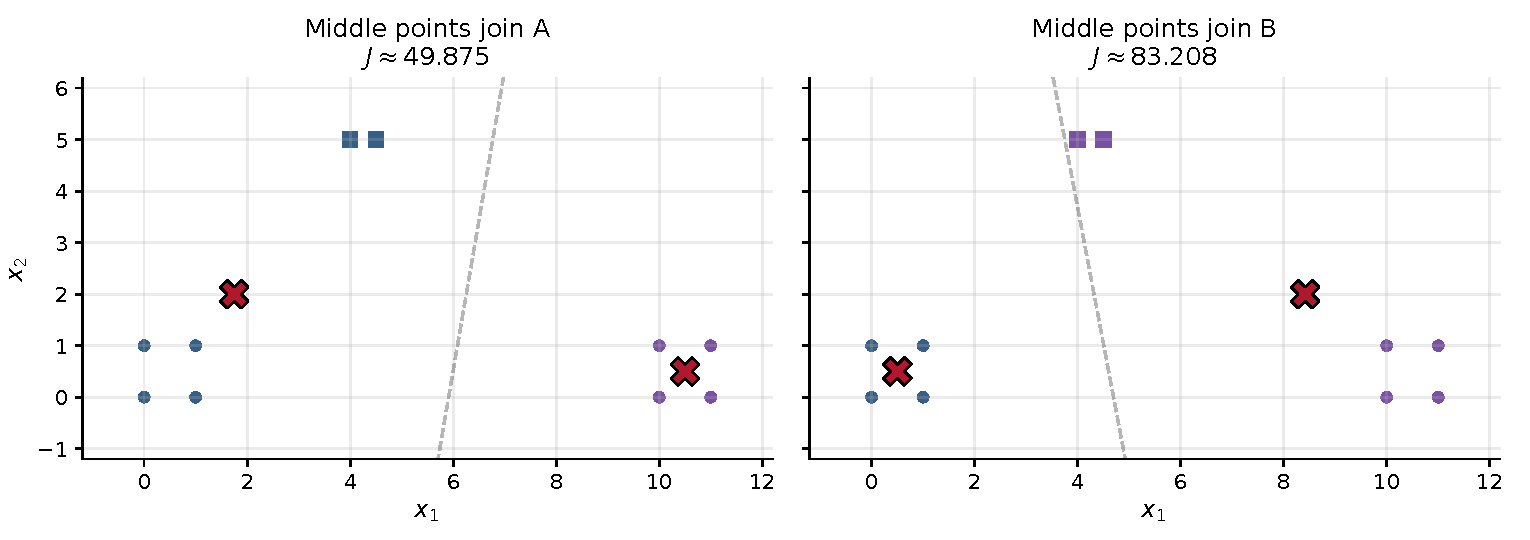
\includegraphics[width=\textwidth]{figures/handouts/em_algorithm/fig_kmeans_fixed_points}
  \caption{A toy $k$-means instance with two stable solutions depending on how the ambiguous ``middle'' points are assigned. Even in this simple setting, the update map has multiple basins and different fixed points can have different objective values.}
  \label{fig:kmeans-fixed-points}
\end{figure}

\Cref{fig:kmeans-fixed-points} makes the basin story visible.
The central points sit near an assignment boundary.
One initialization causes them to be claimed by the left cluster; another causes them to be claimed by the right cluster.
Once those assignments differ, the cluster means move differently, which reinforces the difference on the next E-step.
The stable solutions are therefore \emph{self-consistent latent assignments}.

This is exactly why initialization is part of the method rather than an afterthought.
In latent-variable problems one rarely hopes for a global theorem of the form ``EM converges to the best optimum from everywhere.''
Instead, the practical template is
\begin{algorithm}[H]
  \caption{Two-stage template: initialization + EM refinement}
  \label{alg:two-stage-em}
  \begin{algorithmic}[1]
    \Require Model class and EM operator $M_n$, plus a cheap initializer.
    \Ensure An estimate $\hat\theta$ intended to approximate a good population maximizer.
    \State \textbf{Initialization:} produce one or more candidates $\Theta_0$ (e.g.\ moments/spectral, $k$-means++, random restarts).
    \State Pick $\theta^{(0)}\in\Theta_0$ using a simple score (e.g.\ likelihood, held-out likelihood, or a surrogate).
    \State \textbf{Refinement:} run EM iterations $\theta^{(t+1)}=M_n(\theta^{(t)})$ until convergence; return the final iterate $\hat\theta$.
  \end{algorithmic}
\end{algorithm}

The Gaussian-mixture example later keeps the same logic but replaces hard assignments by soft responsibilities.
That makes the map smooth enough to analyze with derivatives, while preserving the same basin-versus-rate distinction.

\section[Gaussian mixture]{Example II: a two-component Gaussian mixture}
\label{sec:gmm-pop-em}

We now illustrate the contractive-map picture in the simplest EM setting: a balanced two-component Gaussian mixture with known variance.
To keep notation light, we work in one dimension and parameterize the unknown mean as $\theta^\star>0$; the model is
\[
Y \sim \tfrac12\,\mathcal{N}(\theta^\star,\sigma^2) + \tfrac12\,\mathcal{N}(-\theta^\star,\sigma^2),
\]
and we estimate $\theta\in\R$.
The latent variable is the component label.
This model makes the basin picture and the local-rate picture visible in the same calculation.
The same explicit map will explain why sign determines the basin and why separation controls the slope.

\subsection{EM operator and fixed points}
\label{subsec:gmm-em-operator}

Given a sample $\{y_i\}_{i=1}^n$, EM alternates between responsibilities
$w_\theta(y_i)=\Pr(Z=+1\mid Y=y_i,\theta)$ and maximizing the resulting quadratic surrogate $Q_n(\theta'\mid\theta)$.
In this model both steps have closed forms, so the update map is one-dimensional and explicit.

\subsubsection{Deriving the EM update in closed form}
\label{subsubsec:gmm-derivation}

We parameterize the mixture using a latent label $Z\in\{-1,+1\}$ with $\Pr(Z=+1)=\Pr(Z=-1)=1/2$ and
\[
Y\mid Z=z,\theta' \sim \mathcal{N}(z\theta',\sigma^2).
\]
The complete-data log-likelihood is (up to constants)
\[
\log f_{\theta'}(y,z) = -\frac{1}{2\sigma^2}\big(y-z\theta'\big)^2.
\]
By Bayes' rule, the responsibility is
\begin{align*}
w_\theta(y)
&=\Pr(Z=+1\mid Y=y,\theta)
=\frac{\exp\!\left(-\frac{(y-\theta)^2}{2\sigma^2}\right)}{\exp\!\left(-\frac{(y-\theta)^2}{2\sigma^2}\right)+\exp\!\left(-\frac{(y+\theta)^2}{2\sigma^2}\right)} \\
&=\frac{1}{1+\exp\!\left(-\frac{(y+\theta)^2-(y-\theta)^2}{2\sigma^2}\right)}
=\frac{1}{1+\exp\!\left(-\frac{2\theta y}{\sigma^2}\right)}.
\end{align*}
Here $(y+\theta)^2-(y-\theta)^2=4\theta y$, so the responsibility is a logistic function of $\theta y/\sigma^2$.
Equivalently,
\[
2w_\theta(y)-1 = \tanh\!\left(\frac{\theta y}{\sigma^2}\right),
\]
so the ``soft label'' $2w_\theta(y)-1$ is a smooth odd function of the score $\theta y$.

The sample $Q$-function is the conditional expectation of the complete-data log-likelihood,
\[
Q_n(\theta'\mid\theta)
=
-\frac{1}{2n\sigma^2}\sum_{i=1}^n\Big(
w_\theta(y_i)\,(y_i-\theta')^2 + (1-w_\theta(y_i))\,(y_i+\theta')^2
\Big),
\]
which is a concave quadratic function of $\theta'$.
Differentiate and set the derivative equal to $0$:
\[
0
=
\frac{\partial}{\partial \theta'}Q_n(\theta'\mid\theta)
=
\frac{1}{n\sigma^2}\sum_{i=1}^n\Big(
w_\theta(y_i)\,(y_i-\theta') - (1-w_\theta(y_i))\,(y_i+\theta')
\Big).
\]
Rearrange the term inside the sum as
\[
w_\theta(y_i)\,(y_i-\theta') - (1-w_\theta(y_i))\,(y_i+\theta')
=
\big(2w_\theta(y_i)-1\big)\,y_i-\theta',
\]
so the first-order condition becomes $0=\frac{1}{n\sigma^2}\sum_{i=1}^n\big(\big(2w_\theta(y_i)-1\big)\,y_i-\theta'\big)$.
Solving for $\theta'$ yields the closed-form M-step
\[
M_n(\theta)
=
\frac{1}{n}\sum_{i=1}^n \big(2w_\theta(y_i)-1\big)\,y_i
=
\frac{1}{n}\sum_{i=1}^n y_i\,\tanh\!\left(\frac{\theta y_i}{\sigma^2}\right).
\]
At the population level, the sample average is replaced by an expectation:
\[
M(\theta)
=
\E\!\left[\big(2w_\theta(Y)-1\big)\,Y\right]
=
\E\!\left[Y\,\tanh\!\left(\frac{\theta Y}{\sigma^2}\right)\right],
\]
yielding a deterministic update map $\theta^{t+1}=M(\theta^t)$.
This formula makes the geometry visible.
The score $\theta Y$ determines the posterior sign of the latent label, and the hyperbolic tangent turns that score into a soft label in $[-1,1]$.
When the mixture components are well separated, most draws of $Y$ make $\theta Y/\sigma^2$ large in magnitude, so the soft labels are close to $\pm 1$ and EM behaves almost like a hard assignment step.
When the components are weakly separated, the same soft labels stay closer to $0$, so the map lies nearer the diagonal and refinement is slower.

\begin{lemma}[Population fixed points for the symmetric mixture]
\label{lem:gmm-fixed-points}
Under the population model $Y=Z\theta^\star+\varepsilon$ with $Z\in\{-1,+1\}$ uniform and $\varepsilon\sim \mathcal{N}(0,\sigma^2)$ independent of $Z$, the population EM map satisfies
\[
M(\theta^\star)=\theta^\star,
\qquad
M(-\theta^\star)=-\theta^\star,
\qquad
M(0)=0.
\]
\end{lemma}

\begin{proof}
For any $\theta$, the posterior mean of the label is
\[
\E[Z\mid Y=y,\theta]
= (+1)\Pr(Z=+1\mid y,\theta) + (-1)\Pr(Z=-1\mid y,\theta)
=2w_\theta(y)-1.
\]
Therefore $M(\theta)=\E\!\left[Y\,\E[Z\mid Y,\theta]\right]$.
At $\theta=\theta^\star$, the conditional expectation is taken under the true model, so by the tower property
\[
M(\theta^\star)
=\E\!\left[Y\,\E[Z\mid Y,\theta^\star]\right]
=\E[YZ].
\]
Since $Y=Z\theta^\star+\varepsilon$ with $\varepsilon\perp Z$ and $Z^2=1$, we have $\E[YZ]=\E[(Z\theta^\star+\varepsilon)Z]=\theta^\star$.
The identity $M(-\theta^\star)=-\theta^\star$ follows by the same argument (or by symmetry of the model), and $M(0)=0$ follows because $w_0(y)=1/2$ so $2w_0(y)-1=0$.
\end{proof}

In this example the geometry assumption in \Cref{thm:em-fos-implies-contraction} is immediate:
the population objective $q(\theta')=Q(\theta'\mid\theta^\star)$ is a concave quadratic in $\theta'$ with second derivative $q''(\theta')=-1/\sigma^2$, hence it is globally $(1/\sigma^2)$-strongly concave.
The remaining step is to verify that the update map is stable in the basin of interest, which in one dimension reduces to controlling the slope $|M'(\theta)|$.

The third fixed point at $0$ plays a different role.
It is a self-consistent point in the sense that perfectly ambiguous responsibilities stay ambiguous, but it is not attractive.
The next exercise computes that instability directly.

\begin{exercise}[Instability of the zero fixed point in the Gaussian mixture map]
\label{ex:gmm-zero-unstable}
Consider the population EM map
\[
M(\theta)=\E\!\left[Y\,\tanh\!\left(\frac{\theta Y}{\sigma^2}\right)\right],
\qquad
Y=Z\theta^\star+\varepsilon,\ Z\in\{-1,+1\}\text{ uniform},\ \varepsilon\sim\mathcal{N}(0,\sigma^2).
\]
\begin{enumerate}[leftmargin=*]
  \item Show that $M$ is an odd function: $M(-\theta)=-M(\theta)$.
  \item Differentiate under the expectation to show
  \[
  M'(\theta)=\E\!\left[\frac{Y^2}{\sigma^2}\cdot \frac{1}{\cosh^2\!\left(\frac{\theta Y}{\sigma^2}\right)}\right].
  \]
  \item Compute $M'(0)$ and conclude that $0$ is a locally unstable fixed point (i.e.\ $|M'(0)|>1$).
\end{enumerate}
\end{exercise}

\SolutionBox[14]{%
\emph{Part (1).}
Using that $\tanh$ is odd,
\[
M(-\theta)
=\E\!\left[Y\,\tanh\!\left(-\frac{\theta Y}{\sigma^2}\right)\right]
=-\E\!\left[Y\,\tanh\!\left(\frac{\theta Y}{\sigma^2}\right)\right]
=-M(\theta).
\]

\emph{Part (2).}
Since $\frac{d}{du}\tanh(u)=\cosh^{-2}(u)$ and $\tanh,\cosh^{-2}$ are bounded, dominated convergence justifies differentiation under the expectation:
\[
M'(\theta)
=\E\!\left[Y\cdot \frac{Y}{\sigma^2}\cdot \frac{1}{\cosh^2\!\left(\frac{\theta Y}{\sigma^2}\right)}\right]
=\E\!\left[\frac{Y^2}{\sigma^2}\cdot \frac{1}{\cosh^2\!\left(\frac{\theta Y}{\sigma^2}\right)}\right].
\]

\emph{Part (3).}
At $\theta=0$, $\cosh^2(0)=1$, so $M'(0)=\E[Y^2]/\sigma^2$.
Under $Y=Z\theta^\star+\varepsilon$ with $Z^2=1$ and $\varepsilon\perp Z$,
\[
\E[Y^2]=\E[(Z\theta^\star+\varepsilon)^2]=(\theta^\star)^2+\sigma^2,
\]
so
\[
M'(0)=\frac{(\theta^\star)^2+\sigma^2}{\sigma^2}=1+\left(\frac{\theta^\star}{\sigma}\right)^2>1.
\]
Hence $0$ is a locally unstable fixed point.%
}

\Cref{fig:em-operator-fixed-points} now has a precise interpretation:
the graph shown there is exactly the map derived above.
The fixed points are its intersections with the diagonal.
Because the model is symmetric, the population log-likelihood has two equivalent maximizers $\pm\theta^\star$, and the sign of the initialization determines which one the iterates approach.
Here that nonconvexity is benign: the two limits differ only by label swapping, so they represent the same fitted mixture distribution.
Larger separation does not change the basin picture; it changes the rate of refinement within each basin.

\subsubsection{Global convergence of population EM in one dimension}
\label{subsubsec:gmm-global-population}

\Cref{fig:em-operator-fixed-points} suggests something stronger than local contraction near $\pm\theta^\star$: in one dimension, every initialization with the correct sign appears to converge to the corresponding population maximizer.
This is true, and it is a rare example where population EM admits a clean global guarantee.

To connect this claim with the literature, write the update map as a two-argument function.
For any $m>0$, let
\[
Y_m \sim \tfrac12\,\mathcal{N}(m,\sigma^2) + \tfrac12\,\mathcal{N}(-m,\sigma^2),
\qquad
M(\theta; m)\coloneqq \E\!\left[Y_m\,\tanh\!\left(\frac{\theta Y_m}{\sigma^2}\right)\right].
\]
Our population EM map is $\theta\mapsto M(\theta;\theta^\star)$, and (by the fixed point lemma) $M(m;m)=m$.

\begin{proposition}[Sign determines the basin in the 1D symmetric mixture]
\label{prop:gmm-global-population-sign-basin}
Assume $\theta^\star>0$.
Let $\theta^{(t+1)}=M(\theta^{(t)};\theta^\star)$ be the population EM iterates.
If $\theta^{(0)}>0$, then $\theta^{(t)}>0$ for all $t$ and $\theta^{(t)}\to \theta^\star$.
By symmetry, if $\theta^{(0)}<0$ then $\theta^{(t)}\to -\theta^\star$, and if $\theta^{(0)}=0$ then $\theta^{(t)}=0$ for all $t$.
\end{proposition}

\begin{proof}
If $\theta>0$, then $y\tanh(\theta y/\sigma^2)\ge 0$ for every $y$, with strict inequality for every $y\neq 0$.
Hence $M(\theta;\theta^\star)>0$, so positive initializations remain positive under the iteration.
The convergence claims are then exactly the one-dimensional specialization of \citet[Thms.~1--2]{xu_hsu_maleki_2016_global_em}: in one dimension, the sign condition $\ip{\theta^{(0)}}{\theta^\star}\gtrless 0$ reduces to $\theta^{(0)}\gtrless 0$, so the cited theorem says the population iterates converge to the corresponding signed maximizer, while the zero initialization remains at the unstable fixed point $0$.
\end{proof}

The same reference proves the higher-dimensional analogue, where the basin is determined by the sign of the inner product $\ip{\theta^{(0)}}{\theta^\star}$ rather than by the sign of a scalar initialization; see \citet[Thms.~1--2]{xu_hsu_maleki_2016_global_em}.

In one dimension, local contractivity near a fixed point is captured by the slope $|M'(\theta^\star)|$: smaller slope means faster refinement.
Since $M(\theta)=\E\!\left[Y\tanh\!\left(\frac{\theta Y}{\sigma^2}\right)\right]$ and $\frac{d}{du}\tanh(u)=\frac{1}{\cosh^2(u)}$, we can differentiate under the expectation to get
\[
M'(\theta)
=
\E\!\left[\frac{Y^2}{\sigma^2}\cdot \frac{1}{\cosh^2\!\left(\frac{\theta Y}{\sigma^2}\right)}\right].
\]
\Cref{fig:em-contraction-vs-snr} plots this slope as a function of the signal-to-noise ratio $\theta^\star/\sigma$ for the Gaussian mixture.
Separation plays the role of a \emph{conditioning parameter} for EM: when $\theta^\star/\sigma$ is large, responsibilities are close to $0$--$1$ under the true model and the map is strongly contractive, so refinement is fast; when $\theta^\star/\sigma$ is small, responsibilities stay near $1/2$ and the slope approaches $1$, so linear convergence becomes extremely slow.
Importantly, this ``slow EM'' regime is not a mysterious algorithmic failure---it reflects the fact that the statistical model itself becomes less distinctive as $\theta^\star/\sigma\to 0$:
the mixture distribution approaches a single Gaussian, so many parameter values yield almost the same observed-data likelihood and there is little signal for any method to exploit.
In other words, low separation is often ``easy'' in a \emph{model-fit} sense (many parameter values fit about equally well), but ``hard'' in a \emph{parameter-estimation} sense (it is difficult to reliably recover the tiny component separation).

\begin{lemma}[A simple sufficient condition for local contractivity]
\label{lem:gmm-contractive-region}
For any $\theta\neq 0$, the derivative satisfies
\[
0< M'(\theta) \le \frac{4e^{-2}\sigma^2}{\theta^2}.
\]
In particular, if $\theta^\star \ge \frac{4\sigma}{e}$, then $M$ is a contraction on the interval $\big[\frac{\theta^\star}{2},\frac{3\theta^\star}{2}\big]$ with contraction factor
\[
\kappa \le \frac{16e^{-2}\sigma^2}{(\theta^\star)^2} < 1.
\]
\end{lemma}

\clearpage
\begin{exercise}[Proving \Cref{lem:gmm-contractive-region}]
\label{ex:gmm-contractive-region}
Prove \Cref{lem:gmm-contractive-region}.
\emph{Hint:} start from $M'(\theta)=\E\!\left[\frac{Y^2}{\sigma^2}\cosh^{-2}\!\left(\frac{\theta Y}{\sigma^2}\right)\right]$,
use $\cosh(u)\ge \tfrac12 e^{|u|}$, and then maximize $y^2e^{-by}$ over $y\ge 0$ for $b>0$.
\end{exercise}

\SolutionBox[22]{%
Starting from
\[
M'(\theta)
=
\E\!\left[\frac{Y^2}{\sigma^2}\cdot \frac{1}{\cosh^2\!\left(\frac{\theta Y}{\sigma^2}\right)}\right],
\]
use $\cosh(u)\ge \tfrac12 e^{|u|}$ to obtain $\cosh^{-2}(u)\le 4e^{-2|u|}$.
Hence,
\[
M'(\theta)
\le
\frac{4}{\sigma^2}\E\!\left[Y^2\exp\!\left(-\frac{2|\theta|\,|Y|}{\sigma^2}\right)\right].
\]
Fix $b>0$.  For $y\ge 0$, the function $y\mapsto y^2e^{-by}$ has derivative $e^{-by}(2y-by^2)$, so it is maximized at $y=2/b$ with value $4e^{-2}/b^2$.
Therefore $Y^2e^{-b|Y|}\le 4e^{-2}/b^2$ almost surely, and with $b=\frac{2|\theta|}{\sigma^2}$ we get
\[
M'(\theta)
\le
\frac{4}{\sigma^2}\cdot \frac{4e^{-2}}{b^2}
=
\frac{4e^{-2}\sigma^2}{\theta^2}.
\]
If $\theta^\star\ge \frac{4\sigma}{e}$ and $\theta\in[\theta^\star/2,3\theta^\star/2]$, then $|\theta|\ge \theta^\star/2$ and the bound gives
\[
\sup_{\theta\in[\theta^\star/2,3\theta^\star/2]} M'(\theta)
\le
\frac{16e^{-2}\sigma^2}{(\theta^\star)^2}
<1,
\]
so $M$ is a contraction on this interval with contraction factor $\kappa\le 16e^{-2}\sigma^2/(\theta^\star)^2$.%
}

\begin{figure}[t]
  \centering
  \begin{tikzpicture}
  \begin{axis}[
    width=0.78\linewidth,
    height=5.8cm,
    xmin=0, xmax=3,
    ymin=0, ymax=1.02,
    axis lines=left,
    xlabel={$\theta^\star/\sigma$},
    ylabel={local slope $|M'(\theta^\star)|$},
    title={Gaussian mixture: contractivity strengthens with separation},
    title style={font=\small, yshift=-0.35em},
    clip=false,
  ]
    \addplot[stat221Blue,thick] table[row sep=\\] {
x y \\
0.000000 1 \\
0.020000 0.999200639318 \\
0.040000 0.996810196552 \\
0.060000 0.99285134851 \\
0.080000 0.987361104747 \\
0.100000 0.980389691245 \\
0.120000 0.971999101273 \\
0.140000 0.962261408213 \\
0.160000 0.951256940118 \\
0.180000 0.939072410763 \\
0.200000 0.925799089615 \\
0.220000 0.911531076495 \\
0.240000 0.896363728474 \\
0.260000 0.880392269087 \\
0.280000 0.863710594595 \\
0.300000 0.846410279611 \\
0.320000 0.828579775021 \\
0.340000 0.810303784702 \\
0.360000 0.791662803511 \\
0.380000 0.772732797077 \\
0.400000 0.753585003412 \\
0.420000 0.734285836967 \\
0.440000 0.714896877044 \\
0.460000 0.695474924141 \\
0.480000 0.676072109754 \\
0.500000 0.656736047028 \\
0.520000 0.637510011546 \\
0.540000 0.618433143276 \\
0.560000 0.599540662238 \\
0.580000 0.580864091861 \\
0.600000 0.562431485194 \\
0.620000 0.544267650154 \\
0.640000 0.526394370884 \\
0.660000 0.50883062299 \\
0.680000 0.491592781046 \\
0.700000 0.474694817242 \\
0.720000 0.45814849041 \\
0.740000 0.44196352504 \\
0.760000 0.426147780064 \\
0.780000 0.41070740746 \\
0.800000 0.395647000799 \\
0.820000 0.380969734022 \\
0.840000 0.36667749078 \\
0.860000 0.352770984743 \\
0.880000 0.339249871297 \\
0.900000 0.326112851098 \\
0.920000 0.313357765928 \\
0.940000 0.300981687329 \\
0.960000 0.288980998447 \\
0.980000 0.277351469548 \\
1.000000 0.266088327605 \\
1.020000 0.255186320385 \\
1.040000 0.244639775404 \\
1.060000 0.234442654114 \\
1.080000 0.224588601677 \\
1.100000 0.215070992637 \\
1.120000 0.205882972786 \\
1.140000 0.197017497522 \\
1.160000 0.188467366949 \\
1.180000 0.180225257954 \\
1.200000 0.17228375351 \\
1.220000 0.164635369393 \\
1.240000 0.157272578521 \\
1.260000 0.150187833083 \\
1.280000 0.143373584641 \\
1.300000 0.136822302343 \\
1.320000 0.130526489398 \\
1.340000 0.124478697942 \\
1.360000 0.118671542426 \\
1.380000 0.11309771162 \\
1.400000 0.107749979356 \\
1.420000 0.102621214102 \\
1.440000 0.097704387443 \\
1.460000 0.0929925815757 \\
1.480000 0.0884789958711 \\
1.500000 0.0841569525892 \\
1.520000 0.0800199018077 \\
1.540000 0.0760614256251 \\
1.560000 0.0722752416963 \\
1.580000 0.0686552061522 \\
1.600000 0.0651953159532 \\
1.620000 0.0618897107203 \\
1.640000 0.0587326740874 \\
1.660000 0.0557186346124 \\
1.680000 0.052842166284 \\
1.700000 0.0500979886587 \\
1.720000 0.0474809666585 \\
1.740000 0.044986110062 \\
1.760000 0.0426085727134 \\
1.780000 0.0403436514783 \\
1.800000 0.0381867849676 \\
1.820000 0.0361335520504 \\
1.840000 0.0341796701761 \\
1.860000 0.0323209935227 \\
1.880000 0.0305535109896 \\
1.900000 0.0288733440535 \\
1.920000 0.027276744506 \\
1.940000 0.0257600920913 \\
1.960000 0.0243198920608 \\
1.980000 0.0229527726556 \\
2.000000 0.0216554825256 \\
2.020000 0.0204248880892 \\
2.040000 0.019257970835 \\
2.060000 0.0181518245719 \\
2.080000 0.017103652636 \\
2.100000 0.0161107650723 \\
2.120000 0.0151705758106 \\
2.140000 0.0142805998594 \\
2.160000 0.0134384505301 \\
2.180000 0.0126418366964 \\
2.200000 0.0118885600784 \\
2.220000 0.0111765125314 \\
2.240000 0.0105036733215 \\
2.260000 0.00986810637488 \\
2.280000 0.00926795751283 \\
2.300000 0.00870145169878 \\
2.320000 0.00816689034165 \\
2.340000 0.00766264869717 \\
2.360000 0.00718717339248 \\
2.380000 0.00673898006967 \\
2.400000 0.00631665111137 \\
2.420000 0.00591883339061 \\
2.440000 0.0055442359866 \\
2.460000 0.00519162783269 \\
2.480000 0.00485983530513 \\
2.500000 0.00454773980721 \\
2.520000 0.00425427543351 \\
2.540000 0.00397842680007 \\
2.560000 0.00371922709277 \\
2.580000 0.00347575632804 \\
2.600000 0.00324713975739 \\
2.620000 0.00303254630428 \\
2.640000 0.00283118691814 \\
2.660000 0.00264231277163 \\
2.680000 0.00246521330105 \\
2.700000 0.00229921417106 \\
2.720000 0.00214367530193 \\
2.740000 0.001997989106 \\
2.760000 0.00186157903248 \\
2.780000 0.00173389843058 \\
2.800000 0.00161442964015 \\
2.820000 0.00150268314598 \\
2.840000 0.00139819661532 \\
2.860000 0.00130053368832 \\
2.880000 0.00120928249346 \\
2.900000 0.00112405397779 \\
2.920000 0.00104448023229 \\
2.940000 0.000970213019799 \\
2.960000 0.000900922663713 \\
2.980000 0.00083629734512 \\
3.000000 0.000776042723369 \\
    };

    \addplot[only marks,mark=*,mark size=1.3pt,stat221Orange] coordinates {
      (0.600000,0.562431485194)
      (2.000000,0.0216554825256)
    };
    \node[font=\small,anchor=south east] at (axis cs:0.600000,0.562431485194) {0.6};
    \node[font=\small,anchor=south west] at (axis cs:2.000000,0.0216554825256) {2};
  \end{axis}
\end{tikzpicture}

  \caption{Local contraction factor $|M'(\theta^\star)|$ for population EM in the symmetric two-component Gaussian mixture, as a function of the signal-to-noise ratio $\theta^\star/\sigma$. Larger separation leads to much stronger contractivity near the population maximizer, hence faster refinement once initialized in the correct basin.}
  \label{fig:em-contraction-vs-snr}
\end{figure}

\subsection{Local theory near a good fixed point}
\label{subsec:em-population-contractivity-template}

The Gaussian-mixture example already contains the shape of a general EM theorem.
Likelihood ascent is only part of the story.
It says that EM does not decrease the observed-data likelihood, but it does not say whether the initialization lies in the basin of a desirable fixed point, whether the population map pulls the iterates back once they are near that point, or whether finite-sample noise distorts that picture.
That is why useful EM results are usually local.

To study the local behavior near a good population fixed point $\theta^\star$, freeze the second argument of the surrogate at $\theta^\star$ and define
\[
q(\theta') \coloneqq Q(\theta' \mid \theta^\star).
\]
This is the surrogate EM would maximize if the E-step already used the correct posterior law.
From that viewpoint, the local theory is built out of two ideas.
First, the ideal objective $q$ should have enough curvature near $\theta^\star$ that maximizing it would correct small perturbations away from the target.
Second, the E-step should be stable: replacing $\theta^\star$ by a nearby iterate $\theta$ should not change the surrogate gradient too much.
If both statements hold, then the true EM map behaves like a perturbed maximization of $q$, so one can prove contraction for the population map and then transfer that result to the sample map by a perturbation argument.
The next definitions write those two ideas in a form suitable for the proof.

\begin{definition}[Local strong concavity]
\label{def:em-local-strong-concavity}
Fix $r>0$ and define the ball $B_r(\theta^\star)\coloneqq\{\theta\in\Theta:\norm{\theta-\theta^\star}_2\le r\}$.
We say $q$ is \textbf{$\lambda$-strongly concave on $B_r(\theta^\star)$} if for all $\theta_1,\theta_2\in B_r(\theta^\star)$,
\[
q(\theta_1)
\le
q(\theta_2)
\;+\;
\ip{\nabla q(\theta_2)}{\theta_1-\theta_2}
\;-\;
\frac{\lambda}{2}\norm{\theta_1-\theta_2}_2^2.
\]
\end{definition}

\begin{definition}[First-order stability (FOS)]
\label{def:em-fos}
Fix $r>0$.
We say the population $Q$-functions satisfy \textbf{$\mathrm{FOS}(\gamma)$ on $B_r(\theta^\star)$} if for all $\theta\in B_r(\theta^\star)$,
\[
\norm{\nabla_{\theta'} Q(M(\theta)\mid \theta^\star)-\nabla_{\theta'} Q(M(\theta)\mid \theta)}_2
\le
\gamma \norm{\theta-\theta^\star}_2.
\]
\end{definition}

\begin{theorem}[FOS + strong concavity $\Rightarrow$ contraction of population EM]
\label{thm:em-fos-implies-contraction}
Fix $r>0$ and define $B_r(\theta^\star)$ as in \Cref{def:em-local-strong-concavity}.
Assume:
\begin{enumerate}[leftmargin=*]
  \item $\theta^\star$ is self-consistent, meaning $M(\theta^\star)=\theta^\star$.
  \item $q(\cdot)=Q(\cdot\mid\theta^\star)$ is $\lambda$-strongly concave on $B_r(\theta^\star)$.
  \item $\mathrm{FOS}(\gamma)$ holds on $B_r(\theta^\star)$ for some $\gamma\in[0,\lambda)$.
  \item For all $\theta\in B_r(\theta^\star)$, the update $M(\theta)$ also lies in $B_r(\theta^\star)$.
  \item $\theta^\star$ is an interior maximizer of $q$, and for each $\theta\in B_r(\theta^\star)$ the EM update $M(\theta)$ is an interior maximizer of $\theta'\mapsto Q(\theta'\mid\theta)$, so that
  \[
  \nabla q(\theta^\star)=0,
  \qquad
  \nabla_{\theta'} Q(M(\theta)\mid\theta)=0.
  \]
\end{enumerate}
Then $M$ is contractive on $B_r(\theta^\star)$ with contraction factor $\kappa=\gamma/\lambda$:
\[
\norm{M(\theta)-\theta^\star}_2
\le
\frac{\gamma}{\lambda}\norm{\theta-\theta^\star}_2
\qquad\text{for all }\theta\in B_r(\theta^\star).
\]
\end{theorem}

\begin{proof}
Fix $\theta\in B_r(\theta^\star)$ and write $\bar\theta \coloneqq M(\theta)$.
By local invariance, $\bar\theta\in B_r(\theta^\star)$.
By \Cref{def:em-local-strong-concavity}, the function $-q$ is $\lambda$-strongly convex on $B_r(\theta^\star)$, so for all $u,v\in B_r(\theta^\star)$,
\[
\ip{\nabla q(u)-\nabla q(v)}{u-v}
\le
-\lambda\norm{u-v}_2^2,
\]
and therefore, by Cauchy--Schwarz,
\[
\lambda\norm{u-v}_2
\le
\norm{\nabla q(u)-\nabla q(v)}_2.
\]
Apply this with $u=\bar\theta$ and $v=\theta^\star$, and use $\nabla q(\theta^\star)=0$, to obtain
\[
\lambda\norm{\bar\theta-\theta^\star}_2
\le
\norm{\nabla q(\bar\theta)}_2
=
\norm{\nabla_{\theta'} Q(\bar\theta\mid\theta^\star)}_2.
\]
By the interior optimality condition $\nabla_{\theta'} Q(\bar\theta\mid\theta)=0$ and $\mathrm{FOS}(\gamma)$,
\[
\norm{\nabla_{\theta'} Q(\bar\theta\mid\theta^\star)}_2
=
\norm{\nabla_{\theta'} Q(\bar\theta\mid\theta^\star)-\nabla_{\theta'} Q(\bar\theta\mid\theta)}_2
\le
\gamma\norm{\theta-\theta^\star}_2.
\]
Combine the last two displays and divide by $\lambda$.
\end{proof}

In words, strong concavity tells us that the ideal M-step would correct deviations from $\theta^\star$, while FOS says the real E-step does not distort that ideal picture too much.
If FOS fails badly, then changing the current iterate can change the posterior weights so much that the update map loses its restorative pull.

\subsubsection{Gradient EM: an inexact M-step}
\label{subsec:em-gradient-em}

In large models, the exact maximization step defining $M(\theta)$ can be expensive.
A common alternative is to take one gradient ascent step on the surrogate $Q(\cdot\mid\theta)$ starting from $\theta$.
At the population level, this defines the \emph{gradient EM} operator
\[
G(\theta)\coloneqq \theta + \alpha\,\nabla_{\theta'} Q(\theta\mid\theta),
\]
where $\alpha>0$ is a step size.
(The sample version replaces $Q$ by $Q_n$.)

If we could take gradient ascent on the ideal objective $q(\theta)=Q(\theta\mid\theta^\star)$ directly, then strong concavity and smoothness would give a contraction for an appropriate step size; see \citep[\S9.2]{boyd_vandenberghe_2004_convex}.
Gradient EM behaves similarly when the surrogate gradient is stable near $\theta^\star$.

\begin{definition}[Gradient stability (GS)]
\label{def:em-gs}
Fix $r>0$.
We say the population $Q$-functions satisfy \textbf{$\mathrm{GS}(\gamma)$ on $B_r(\theta^\star)$} if for all $\theta\in B_r(\theta^\star)$,
\[
\norm{\nabla_{\theta'} Q(\theta\mid \theta^\star)-\nabla_{\theta'} Q(\theta\mid \theta)}_2
\le
\gamma \norm{\theta-\theta^\star}_2.
\]
\end{definition}

\begin{theorem}[GS + strong concavity $\Rightarrow$ contraction of gradient EM]
\label{thm:em-gs-implies-contraction}
Fix $r>0$ and assume:
\begin{enumerate}[leftmargin=*]
  \item $q(\cdot)=Q(\cdot\mid\theta^\star)$ is $\lambda$-strongly concave and $L$-smooth on $B_r(\theta^\star)$, with $0<\lambda\le L$.
  \item $\mathrm{GS}(\gamma)$ holds on $B_r(\theta^\star)$ for some $\gamma\in[0,\lambda)$.
  \item $\theta^\star$ is an interior maximizer of $q$, so $\nabla q(\theta^\star)=0$.
\end{enumerate}
Then gradient EM with step size $\alpha=\frac{2}{L+\lambda}$ is contractive on $B_r(\theta^\star)$:
\[
\norm{G(\theta)-\theta^\star}_2
\le
\left(\frac{L-\lambda+2\gamma}{L+\lambda}\right)\norm{\theta-\theta^\star}_2
\qquad\text{for all }\theta\in B_r(\theta^\star).
\]
\end{theorem}

\begin{proof}
Write $G(\theta)-\theta^\star$ as
\[
\underbrace{\theta + \alpha \nabla q(\theta)-\theta^\star}_{\text{gradient ascent on $q$}}
\;+\;
\alpha\underbrace{\bigl(\nabla_{\theta'} Q(\theta\mid\theta)-\nabla_{\theta'} Q(\theta\mid\theta^\star)\bigr)}_{\text{stability error}}.
\]
For $\alpha=\frac{2}{L+\lambda}$, gradient ascent on a $\lambda$-strongly concave, $L$-smooth function is a contraction mapping with factor $\frac{L-\lambda}{L+\lambda}$ (equivalently, apply the standard strongly convex result to $-q$).
Combine this with \Cref{def:em-gs} and $\alpha=\frac{2}{L+\lambda}$ to get
\[
\norm{G(\theta)-\theta^\star}_2
\le
\left(\frac{L-\lambda}{L+\lambda} + \frac{2\gamma}{L+\lambda}\right)\norm{\theta-\theta^\star}_2,
\]
which is the claim.
\end{proof}

Once a population contraction factor is available for either exact EM or gradient EM, the sample-level picture follows from a perturbation argument.

\begin{lemma}[Contraction + perturbation $\Rightarrow$ convergence to a neighborhood]
\label{lem:contraction-perturbation}
Fix a point $\theta^\star\in\Theta$ and a radius $r>0$.
Assume:
\begin{enumerate}[leftmargin=*]
  \item $M(\theta^\star)=\theta^\star$ and, for all $\theta$ with $\norm{\theta-\theta^\star}_2\le r$,
  \[
  \norm{M(\theta)-\theta^\star}_2 \le \kappa \norm{\theta-\theta^\star}_2
  \quad\text{for some }\kappa\in(0,1).
  \]
  \item For all $\theta$ with $\norm{\theta-\theta^\star}_2\le r$,
  \[
  \norm{M_n(\theta)-M(\theta)}_2 \le \varepsilon_n.
  \]
\end{enumerate}
Then any iterate sequence $\theta^{t+1}=M_n(\theta^t)$ that remains in the ball satisfies
\[
\norm{\theta^t-\theta^\star}_2
\le
\kappa^t \norm{\theta^0-\theta^\star}_2 + \frac{\varepsilon_n}{1-\kappa}.
\]
\end{lemma}

\begin{proof}
Write
\[
\norm{\theta^{t+1}-\theta^\star}_2
\le
\norm{M(\theta^t)-\theta^\star}_2 + \norm{M_n(\theta^t)-M(\theta^t)}_2
\le
\kappa\norm{\theta^t-\theta^\star}_2 + \varepsilon_n,
\]
then unroll the recursion.
\end{proof}

\Cref{lem:contraction-perturbation} is the core population-to-sample message.
Inside a basin where the sample map stays uniformly close to the population map, optimization error decays geometrically until it reaches a floor of order $\varepsilon_n/(1-\kappa)$.
Equivalently, sample EM converges to the sample fixed point in its basin, while the gap between that sample target and the population target is the residual statistical error.

\subsection{Finite-sample EM: geometric decay until a floor}
\label{sec:finite-sample-floor}

At finite $n$, the operator $M_n$ fluctuates around $M$.
In a neighborhood where $M$ is contractive and $M_n$ is uniformly close to $M$, \Cref{lem:contraction-perturbation} gives geometric decay until the remaining error is on the order of $1/\sqrt{n}$.

\begin{figure}[t]
  \centering
  \begin{tikzpicture}
  \begin{axis}[
    width=0.92\linewidth,
    height=6.2cm,
    xmin=0, xmax=22,
    ymode=log,
    axis lines=left,
    xlabel={EM iteration $t$},
    ylabel={distance $|\theta^{(t)}-\theta^\star|$},
    title={Gaussian mixture: geometric refinement until a sample-size floor},
    title style={font=\small, yshift=-0.35em},
    legend style={draw=stat221Gray!25, fill=white, fill opacity=0.95, text opacity=1},
    legend pos=north east,
    clip=false,
  ]
    \addplot[stat221Gray,thick,densely dashed] table[row sep=\\] {
x y \\
0.000000 1.8 \\
1.000000 1.09729288275 \\
2.000000 0.109028376417 \\
3.000000 0.00261865712788 \\
4.000000 5.68444330535e-05 \\
5.000000 1.23073156089e-06 \\
6.000000 2.63256854094e-08 \\
7.000000 2.43660647214e-10 \\
8.000000 3.21158211136e-10 \\
9.000000 3.33389760243e-10 \\
10.000000 3.33654437412e-10 \\
11.000000 3.33660210572e-10 \\
12.000000 3.33660654661e-10 \\
13.000000 3.33660654661e-10 \\
14.000000 3.33660654661e-10 \\
15.000000 3.33660654661e-10 \\
16.000000 3.33660654661e-10 \\
17.000000 3.33660654661e-10 \\
18.000000 3.33660654661e-10 \\
19.000000 3.33660654661e-10 \\
20.000000 3.33660654661e-10 \\
21.000000 3.33660654661e-10 \\
22.000000 3.33660654661e-10 \\
    };
    \addlegendentry{Population EM}

    % n=250
    \addplot[stat221Red,thick] table[row sep=\\] {
x y \\
0.000000 1.8 \\
1.000000 1.09872386901 \\
2.000000 0.110299246121 \\
3.000000 0.0505039018034 \\
4.000000 0.0515472428277 \\
5.000000 0.0515163642603 \\
6.000000 0.0515154249441 \\
7.000000 0.0515153981012 \\
8.000000 0.0515153973593 \\
9.000000 0.0515153973392 \\
10.000000 0.0515153973386 \\
11.000000 0.0515153973386 \\
12.000000 0.0515153973386 \\
13.000000 0.0515153973386 \\
14.000000 0.0515153973386 \\
15.000000 0.0515153973386 \\
16.000000 0.0515153973386 \\
17.000000 0.0515153973386 \\
18.000000 0.0515153973386 \\
19.000000 0.0515153973386 \\
20.000000 0.0515153973386 \\
21.000000 0.0515153973386 \\
22.000000 0.0515153973386 \\
    };
    \addlegendentry{$n=250$ (median)}
    \addplot[stat221Red!50,thin] table[row sep=\\] {
x y \\
0.000000 1.8 \\
1.000000 1.06088484132 \\
2.000000 0.0558003250334 \\
3.000000 0.0172269337719 \\
4.000000 0.0187376939554 \\
5.000000 0.0186938843451 \\
6.000000 0.0186928789526 \\
7.000000 0.0186928558916 \\
8.000000 0.0186928553628 \\
9.000000 0.0186928553507 \\
10.000000 0.0186928553504 \\
11.000000 0.0186928553504 \\
12.000000 0.0186928553504 \\
13.000000 0.0186928553504 \\
14.000000 0.0186928553504 \\
15.000000 0.0186928553504 \\
16.000000 0.0186928553504 \\
17.000000 0.0186928553504 \\
18.000000 0.0186928553504 \\
19.000000 0.0186928553504 \\
20.000000 0.0186928553504 \\
21.000000 0.0186928553504 \\
22.000000 0.0186928553504 \\
    };
    \addplot[stat221Red!50,thin] table[row sep=\\] {
x y \\
0.000000 1.8 \\
1.000000 1.13749626527 \\
2.000000 0.195839244443 \\
3.000000 0.110853135634 \\
4.000000 0.10599630166 \\
5.000000 0.105840011233 \\
6.000000 0.105834999751 \\
7.000000 0.105834838944 \\
8.000000 0.10583483378 \\
9.000000 0.105834833614 \\
10.000000 0.105834833609 \\
11.000000 0.105834833608 \\
12.000000 0.105834833608 \\
13.000000 0.105834833608 \\
14.000000 0.105834833608 \\
15.000000 0.105834833608 \\
16.000000 0.105834833608 \\
17.000000 0.105834833608 \\
18.000000 0.105834833608 \\
19.000000 0.105834833608 \\
20.000000 0.105834833608 \\
21.000000 0.105834833608 \\
22.000000 0.105834833608 \\
    };

    % n=1000
    \addplot[stat221Purple,thick] table[row sep=\\] {
x y \\
0.000000 1.8 \\
1.000000 1.0983030735 \\
2.000000 0.116403226832 \\
3.000000 0.0249846970799 \\
4.000000 0.0271994451237 \\
5.000000 0.0272440273864 \\
6.000000 0.027244923102 \\
7.000000 0.0272449411 \\
8.000000 0.0272449414617 \\
9.000000 0.027244941469 \\
10.000000 0.0272449414691 \\
11.000000 0.0272449414691 \\
12.000000 0.0272449414691 \\
13.000000 0.0272449414691 \\
14.000000 0.0272449414691 \\
15.000000 0.0272449414691 \\
16.000000 0.0272449414691 \\
17.000000 0.0272449414691 \\
18.000000 0.0272449414691 \\
19.000000 0.0272449414691 \\
20.000000 0.0272449414691 \\
21.000000 0.0272449414691 \\
22.000000 0.0272449414691 \\
    };
    \addlegendentry{$n=1000$ (median)}
    \addplot[stat221Purple!55,thin] table[row sep=\\] {
x y \\
0.000000 1.8 \\
1.000000 1.08333007975 \\
2.000000 0.0836193134053 \\
3.000000 0.0103829014241 \\
4.000000 0.00847228156732 \\
5.000000 0.00841108953049 \\
6.000000 0.00840974432263 \\
7.000000 0.00840971474938 \\
8.000000 0.00840971409918 \\
9.000000 0.00840971408488 \\
10.000000 0.00840971408457 \\
11.000000 0.00840971408456 \\
12.000000 0.00840971408456 \\
13.000000 0.00840971408456 \\
14.000000 0.00840971408456 \\
15.000000 0.00840971408456 \\
16.000000 0.00840971408456 \\
17.000000 0.00840971408456 \\
18.000000 0.00840971408456 \\
19.000000 0.00840971408456 \\
20.000000 0.00840971408456 \\
21.000000 0.00840971408456 \\
22.000000 0.00840971408456 \\
    };
    \addplot[stat221Purple!55,thin] table[row sep=\\] {
x y \\
0.000000 1.8 \\
1.000000 1.12615938693 \\
2.000000 0.165376411295 \\
3.000000 0.0472545773638 \\
4.000000 0.0455814764069 \\
5.000000 0.0455189731835 \\
6.000000 0.0455173198223 \\
7.000000 0.0455172765315 \\
8.000000 0.0455172754058 \\
9.000000 0.0455172753767 \\
10.000000 0.0455172753759 \\
11.000000 0.0455172753759 \\
12.000000 0.0455172753759 \\
13.000000 0.0455172753759 \\
14.000000 0.0455172753759 \\
15.000000 0.0455172753759 \\
16.000000 0.0455172753759 \\
17.000000 0.0455172753759 \\
18.000000 0.0455172753759 \\
19.000000 0.0455172753759 \\
20.000000 0.0455172753759 \\
21.000000 0.0455172753759 \\
22.000000 0.0455172753759 \\
    };

    % n=4000
    \addplot[stat221Blue,thick] table[row sep=\\] {
x y \\
0.000000 1.8 \\
1.000000 1.09776860352 \\
2.000000 0.106236150851 \\
3.000000 0.0150328312308 \\
4.000000 0.0136287629058 \\
5.000000 0.0136241329475 \\
6.000000 0.0136239966889 \\
7.000000 0.0136239929464 \\
8.000000 0.0136239928479 \\
9.000000 0.0136239928454 \\
10.000000 0.0136239928454 \\
11.000000 0.0136239928454 \\
12.000000 0.0136239928454 \\
13.000000 0.0136239928454 \\
14.000000 0.0136239928454 \\
15.000000 0.0136239928454 \\
16.000000 0.0136239928454 \\
17.000000 0.0136239928454 \\
18.000000 0.0136239928454 \\
19.000000 0.0136239928454 \\
20.000000 0.0136239928454 \\
21.000000 0.0136239928454 \\
22.000000 0.0136239928454 \\
    };
    \addlegendentry{$n=4000$ (median)}
    \addplot[stat221Blue!55,thin] table[row sep=\\] {
x y \\
0.000000 1.8 \\
1.000000 1.08188882734 \\
2.000000 0.0820973327345 \\
3.000000 0.00770508259319 \\
4.000000 0.0065464756106 \\
5.000000 0.00660028365008 \\
6.000000 0.00660143725538 \\
7.000000 0.00660146199262 \\
8.000000 0.00660146252319 \\
9.000000 0.00660146253458 \\
10.000000 0.00660146253482 \\
11.000000 0.00660146253483 \\
12.000000 0.00660146253483 \\
13.000000 0.00660146253483 \\
14.000000 0.00660146253483 \\
15.000000 0.00660146253483 \\
16.000000 0.00660146253483 \\
17.000000 0.00660146253483 \\
18.000000 0.00660146253483 \\
19.000000 0.00660146253483 \\
20.000000 0.00660146253483 \\
21.000000 0.00660146253483 \\
22.000000 0.00660146253483 \\
    };
    \addplot[stat221Blue!55,thin] table[row sep=\\] {
x y \\
0.000000 1.8 \\
1.000000 1.10460440298 \\
2.000000 0.12368330304 \\
3.000000 0.022890556425 \\
4.000000 0.022627348017 \\
5.000000 0.0226500740391 \\
6.000000 0.0226504929312 \\
7.000000 0.0226505004549 \\
8.000000 0.022650500585 \\
9.000000 0.0226505005871 \\
10.000000 0.0226505005871 \\
11.000000 0.0226505005871 \\
12.000000 0.0226505005871 \\
13.000000 0.0226505005871 \\
14.000000 0.0226505005871 \\
15.000000 0.0226505005871 \\
16.000000 0.0226505005871 \\
17.000000 0.0226505005871 \\
18.000000 0.0226505005871 \\
19.000000 0.0226505005871 \\
20.000000 0.0226505005871 \\
21.000000 0.0226505005871 \\
22.000000 0.0226505005871 \\
    };
  \end{axis}
\end{tikzpicture}

  \caption{Distance to $\theta^\star$ versus EM iteration in the Gaussian mixture example. Population EM converges linearly to $\theta^\star$. Sample EM tracks the population dynamics until it reaches a sample-dependent floor.}
  \label{fig:em-pop-vs-sample}
\end{figure}

In this example, once the initialization lands in the correct basin, the population map is contractive and the sample map tracks it until the iterate reaches an $n$-dependent statistical floor.
Separation does not change which basin is correct; it changes the speed of refinement inside that basin.

A systematic development of this population-to-sample contraction argument appears in \citet[Thm.~1]{balakrishnan_wainwright_yu_2014_em}.
Moreover, this two-Gaussian mixture is one of the rare latent-variable models where much stronger \emph{global} guarantees are possible; see, e.g., \citet[Thm.~1]{xu_hsu_maleki_2016_global_em}.

\clearpage
% ------------------------------------------------------------
\section[Missing covariates]{Example III: regression with missing covariates}
\label{sec:missing-covariates}

EM is also natural outside mixture models whenever part of the data is latent or unobserved.
A basic example is linear regression with covariates missing completely at random.
Let $X\in\R^d$ and $Y\in\R$ follow the population model
\[
X \sim \mathcal{N}(0,I_d),
\qquad
Y = \ip{X}{\theta^\star} + \varepsilon,
\qquad
\varepsilon \sim \mathcal{N}(0,\sigma^2)\ \text{independent of }X,
\]
and suppose we observe $Y$ but only a subset of the coordinates of $X$.
Formally, each coordinate is missing with probability $\rho\in[0,1)$, independently across coordinates and samples.
The missing coordinates are treated as latent variables, so EM alternates between imputing them from the conditional law of $X$ given $(X_{\mathrm{obs}},Y)$ and refitting $\theta'$ by weighted least squares using the conditional moments $\E[X\mid X_{\mathrm{obs}},Y,\theta]$ and $\E[XX^\top\mid X_{\mathrm{obs}},Y,\theta]$.

This example complements the Gaussian mixture.
In the mixture model, weak separation mainly makes the EM map flatter near the correct target.
Here the more basic issue is that the E-step literally fills in unseen coordinates using the \emph{current} parameter.
If $\theta$ is already close to $\theta^\star$, those imputations are helpful.
If $\theta$ points in a badly wrong direction and the missingness level is high, the imputations can reinforce that wrong direction, so the map itself can develop a bad stable fixed point.

\subsection{Missingness and identifiability}
\label{subsec:missing-covariates-identifiability-limit}

As $\rho$ increases, fewer coordinates of $X$ are observed, the E-step becomes less informative, and both optimization and statistical estimation become harder.

The extreme case $\rho=1$ shows the identifiability issue most clearly.
If all covariates are missing, then the observed data are only the responses $\{Y_i\}_{i=1}^n$.
Because $X\sim\mathcal{N}(0,I_d)$, for any parameter $\theta$ we have $\ip{X}{\theta}\sim \mathcal{N}(0,\norm{\theta}_2^2)$, so
\[
Y \mid \theta
\sim
\mathcal{N}\!\big(0,\norm{\theta}_2^2+\sigma^2\big).
\]
Therefore the distribution of the observed data depends on $\theta$ only through $\norm{\theta}_2$.
In particular, the direction of $\theta^\star$ is \emph{not identifiable}: any $\tilde\theta$ with $\norm{\tilde\theta}_2=\norm{\theta^\star}_2$ produces the same law for $Y$.
No algorithm (EM included) can recover what the data do not contain; at best, one can hope to estimate $\norm{\theta^\star}_2$.
\Cref{fig:em-nonidentifiability-ridge} gives a schematic picture.

\begin{figure}[t]
  \centering
  \begin{tikzpicture}
  \begin{axis}[
    width=0.62\linewidth,
    height=6.0cm,
    axis lines=middle,
    xmin=-1.6, xmax=1.6,
    ymin=-1.6, ymax=1.6,
    xlabel={$\theta_1$},
    ylabel={$\theta_2$},
    xtick=\empty,
    ytick=\empty,
    clip=false,
  ]
    \addplot[stat221Blue,thick,domain=0:360,samples=200] ({cos(x)}, {sin(x)});

    \addplot[only marks,mark=*,mark size=1.2pt,stat221Red] coordinates {(1,0)};
    \node[
      font=\small,
      anchor=south west,
      fill=white,
      fill opacity=0.92,
      text opacity=1,
      inner sep=1pt,
      rounded corners=1pt,
    ] at (axis cs:1.050000,0.080000) {$\theta^\star$};

    \addplot[only marks,mark=*,mark size=1.2pt,stat221Purple] coordinates {(0,1)};
    \node[
      font=\small,
      anchor=south east,
      fill=white,
      fill opacity=0.92,
      text opacity=1,
      inner sep=1pt,
      rounded corners=1pt,
    ] at (axis cs:-0.040000,1.070000) {$\tilde\theta$};

    \node[
      font=\small,
      align=center,
      stat221Gray,
      fill=white,
      fill opacity=0.92,
      text opacity=1,
      inner sep=1.5pt,
      rounded corners=1pt,
    ] at (axis cs:0,-1.420000) {same observed law\\(same $\|\theta\|_2$)};
  \end{axis}
\end{tikzpicture}

  \caption{Non-identifiability in the ``noise-only'' limit.  When $\rho=1$, we never observe any coordinates of $X$, and the marginal law is $Y\mid\theta\sim\mathcal{N}(0,\norm{\theta}_2^2+\sigma^2)$.  Hence all parameters on a sphere $\{\theta:\norm{\theta}_2=\text{const}\}$ induce the same distribution of $Y$, so there cannot be a contraction toward a unique maximizer.}
  \label{fig:em-nonidentifiability-ridge}
\end{figure}

This illustrates a different failure mode than low separation in mixtures.
In Example II, low separation mainly means weak identification and poor conditioning: there is a well-defined population target up to the sign symmetry, but the likelihood is relatively flat and the EM contraction factor is close to $1$, so refinement is slow and statistical accuracy requires very large $n$.
Here, increasing missingness pushes the statistical problem itself toward non-identifiability, so EM no longer has a unique population target to contract toward.

\subsection{Deriving the EM operator in closed form}
\label{subsec:missing-covariates-derivation}

Because the model is Gaussian, the E-step conditional moments can be written explicitly and the M-step reduces to a linear system.
These formulas show exactly where the self-reinforcement enters:
the posterior moments used in the E-step depend on the current iterate $\theta$, so the regression problem solved by the M-step is built out of \emph{imputed} covariates that already reflect the current belief.

\subsubsection{E-step: conditional moments from a joint Gaussian}
\label{subsubsec:missing-covariates-estep}

Fix one observation $(x_{\mathrm{obs}},y)$ and let $O\subseteq\{1,\dots,d\}$ be the set of observed coordinates, with $M$ its complement.
Write the parameter and covariate vector in blocks $\theta=(\theta_M,\theta_O)$ and $X=(X_M,X_O)$.
Conditioned on $X_O=x_O$, the scalar response model under parameter $\theta$ is
\[
Y = \ip{\theta_O}{x_O} + \ip{\theta_M}{X_M} + \varepsilon,
\qquad
X_M\sim\mathcal{N}(0,I),
\qquad
\varepsilon\sim\mathcal{N}(0,\sigma^2),
\]
so $X_M\mid (X_O=x_O,Y=y,\theta)$ is the Gaussian posterior in a one-dimensional linear measurement model.
A standard conditioning calculation (e.g.\ via Sherman--Morrison) yields
\begin{align}
\label{eq:missing-covariates-posterior-mean}
\E[X_M\mid x_O,y,\theta]
&=
\frac{\theta_M}{\sigma^2+\norm{\theta_M}_2^2}\,\Big(y-\ip{\theta_O}{x_O}\Big), \\
\label{eq:missing-covariates-posterior-cov}
\mathrm{Cov}(X_M\mid x_O,y,\theta)
&=
I-\frac{\theta_M\theta_M^\top}{\sigma^2+\norm{\theta_M}_2^2}.
\end{align}

Define the conditional mean and second moment of the \emph{full} covariate vector,
\[
\mu_\theta(x_{\mathrm{obs}},y)\coloneqq \E[X\mid X_{\mathrm{obs}}=x_{\mathrm{obs}},Y=y,\theta],
\qquad
\Sigma_\theta(x_{\mathrm{obs}},y)\coloneqq \E[XX^\top\mid X_{\mathrm{obs}}=x_{\mathrm{obs}},Y=y,\theta].
\]
Then $\mu_\theta$ agrees with the observed coordinates and uses \eqref{eq:missing-covariates-posterior-mean} for the missing coordinates:
\[
(\mu_\theta)_O = x_O,
\qquad
(\mu_\theta)_M = \E[X_M\mid x_O,y,\theta].
\]
Similarly, $\Sigma_\theta$ is obtained by combining the posterior covariance \eqref{eq:missing-covariates-posterior-cov} with the rank-one term from the posterior mean:
\[
(\Sigma_\theta)_{MM}
=
\mathrm{Cov}(X_M\mid x_O,y,\theta) + \E[X_M\mid x_O,y,\theta]\E[X_M\mid x_O,y,\theta]^\top,
\qquad
(\Sigma_\theta)_{OO}=x_Ox_O^\top,
\]
and the cross moments satisfy $(\Sigma_\theta)_{MO}=\E[X_M\mid x_O,y,\theta]\,x_O^\top$ and $(\Sigma_\theta)_{OM}=x_O\,\E[X_M\mid x_O,y,\theta]^\top$.

\clearpage
This Gaussian-conditioning algebra is the exact E-step calculation underlying the formulas above.
\begin{exercise}[Deriving the E-step conditional moments in the missing-covariates model]
\label{ex:missing-covariates-estep}
In \Cref{subsubsec:missing-covariates-estep}, fix a set of observed coordinates $O$ with complement $M$, and fix one observation $(x_O,y)$.
Consider the linear-Gaussian model
\[
X_M\sim\mathcal{N}(0,I),
\qquad
Y=\ip{\theta_O}{x_O}+\ip{\theta_M}{X_M}+\varepsilon,
\qquad
\varepsilon\sim\mathcal{N}(0,\sigma^2)\ \text{independent of }X_M.
\]
Show that the posterior is Gaussian with mean and covariance
\[
\E[X_M\mid x_O,y,\theta]=\frac{\theta_M}{\sigma^2+\norm{\theta_M}_2^2}\,\Big(y-\ip{\theta_O}{x_O}\Big),
\qquad
\mathrm{Cov}(X_M\mid x_O,y,\theta)=I-\frac{\theta_M\theta_M^\top}{\sigma^2+\norm{\theta_M}_2^2}.
\]
\emph{Hint:} write $(X_M,\;Y-\ip{\theta_O}{x_O})$ as a jointly Gaussian pair and use the standard conditional Gaussian formula.
\end{exercise}

\SolutionBox[18]{%
This is the standard conditional-Gaussian calculation behind the E-step.
Define the centered scalar $\tilde Y\coloneqq Y-\ip{\theta_O}{x_O}=\ip{\theta_M}{X_M}+\varepsilon$.
Then $(X_M,\tilde Y)$ is jointly Gaussian with
\[
\E[X_M]=0,
\qquad
\E[\tilde Y]=0,
\qquad
\mathrm{Cov}(X_M)=I.
\]
Moreover,
\[
\mathrm{Cov}(X_M,\tilde Y)
=
\E[X_M(\theta_M^\top X_M+\varepsilon)]
=
\E[X_M X_M^\top]\theta_M
=\theta_M,
\]
and
\[
\mathrm{Var}(\tilde Y)
=
\mathrm{Var}(\theta_M^\top X_M)+\mathrm{Var}(\varepsilon)
=
\norm{\theta_M}_2^2+\sigma^2.
\]
For a jointly Gaussian pair $(U,V)$ with $\mathrm{Var}(V)>0$, the conditional law is
\[
U\mid(V=v)\sim \mathcal{N}\!\left(\mathrm{Cov}(U,V)\,\mathrm{Var}(V)^{-1}v,\;\mathrm{Cov}(U)-\mathrm{Cov}(U,V)\,\mathrm{Var}(V)^{-1}\mathrm{Cov}(V,U)\right).
\]
Apply this with $U=X_M$ and $V=\tilde Y$ to obtain
\[
\E[X_M\mid \tilde Y=\tilde y]=\frac{\theta_M}{\sigma^2+\norm{\theta_M}_2^2}\,\tilde y,
\qquad
\mathrm{Cov}(X_M\mid \tilde Y)=I-\frac{\theta_M\theta_M^\top}{\sigma^2+\norm{\theta_M}_2^2}.
\]
Substitute $\tilde y=y-\ip{\theta_O}{x_O}$ to match \eqref{eq:missing-covariates-posterior-mean}--\eqref{eq:missing-covariates-posterior-cov}.%
}
\subsubsection{M-step: a quadratic \texorpdfstring{$Q_n$}{Qn} and a linear system}
\label{subsubsec:missing-covariates-mstep}

The complete-data log-likelihood for a single pair $(x,y)$ is
\[
\log f_{\theta'}(x,y)
=
C
-\frac{1}{2}\norm{x}_2^2
-\frac{1}{2\sigma^2}\big(y-\ip{x}{\theta'}\big)^2.
\]
In the $Q$-function, we take the conditional expectation over the missing covariates under the current iterate $\theta$.
The term $\norm{x}_2^2$ does not depend on $\theta'$, and the factor $1/\sigma^2$ does not affect the argmax, so it is enough to expand the expected squared error.
For one observation,
\begin{align*}
\E\Big[\big(y-\ip{X}{\theta'}\big)^2\mid x_{\mathrm{obs}},y,\theta\Big]
&=
y^2 - 2y\,\ip{\E[X\mid x_{\mathrm{obs}},y,\theta]}{\theta'}
  + \E\big[\theta'^\top XX^\top \theta'\mid x_{\mathrm{obs}},y,\theta\big] \\
&=
y^2 - 2y\,\ip{\mu_\theta(x_{\mathrm{obs}},y)}{\theta'}
  + \theta'^\top \Sigma_\theta(x_{\mathrm{obs}},y)\,\theta'.
\end{align*}
Summing over samples, and dropping additive constants that do not affect the maximizer, yields the quadratic form
\[
Q_n(\theta'\mid\theta)
=
-\frac{1}{2n}\sum_{i=1}^n
\Big(\theta'^\top \Sigma_\theta(x_{\mathrm{obs},i},y_i)\,\theta'
-2y_i\,\ip{\mu_\theta(x_{\mathrm{obs},i},y_i)}{\theta'}\Big).
\]
Taking a gradient in $\theta'$ and setting it equal to zero gives a linear system for the M-step:
\[
\left(\frac{1}{n}\sum_{i=1}^n \Sigma_\theta(x_{\mathrm{obs},i},y_i)\right)\theta'
=
\frac{1}{n}\sum_{i=1}^n y_i\,\mu_\theta(x_{\mathrm{obs},i},y_i),
\]
so, whenever the averaged conditional second-moment matrix is invertible, the unique sample M-step is
\[
M_n(\theta)
=
\left(\frac{1}{n}\sum_{i=1}^n \Sigma_\theta(x_{\mathrm{obs},i},y_i)\right)^{-1}
\left(\frac{1}{n}\sum_{i=1}^n y_i\,\mu_\theta(x_{\mathrm{obs},i},y_i)\right).
\]
The population operator $M$ has the same form with empirical averages replaced by expectations, again when the corresponding population matrix is nonsingular.
Here the relationship between $M$ and $M_n$ is direct: $M_n$ is the perturbation produced by replacing expectations with sample averages.

As a useful check, if there is no missingness ($\rho=0$), then $\mu_\theta(x_{\mathrm{obs}},y)=x$ and $\Sigma_\theta(x_{\mathrm{obs}},y)=xx^\top$ regardless of $\theta$, so $M_n(\theta)$ reduces to ordinary least squares and does not depend on the current iterate.

\subsubsection{A one-dimensional verification: explicit population map and local slope}
\label{subsubsec:missing-covariates-1d-check}

The full verification of contractivity for the missing-covariates model is algebraically involved in general dimension.
In one dimension the population EM map has a closed form, so the stability calculation can be carried out directly.
As in the Gaussian mixture, the population objective $q(\theta')=Q(\theta'\mid\theta^\star)$ is a concave quadratic in $\theta'$ with Hessian $-\sigma^{-2}I$, so the main issue is not the local geometry of $q$ but the stability of the E-step as $\theta$ varies.

Assume $d=1$.
Each sample either reveals $X$ (with probability $1-\rho$) or hides it (with probability $\rho$), and we always observe $Y=\theta^\star X+\varepsilon$.
When $X$ is missing, the E-step uses the Gaussian posterior under the current iterate $\theta$:
\[
X\mid (Y=y,\theta) \sim \mathcal{N}\!\left(\frac{\theta}{\theta^2+\sigma^2}y,\;\frac{\sigma^2}{\theta^2+\sigma^2}\right),
\]
so
\[
\mu_\theta(y) \coloneqq \E[X\mid Y=y,\theta] = \frac{\theta}{\theta^2+\sigma^2}y,
\qquad
\Sigma_\theta(y) \coloneqq \E[X^2\mid Y=y,\theta]
=
\frac{\sigma^2}{\theta^2+\sigma^2}+\mu_\theta(y)^2.
\]
When $X$ is observed, we simply have $\mu_\theta(x,y)=x$ and $\Sigma_\theta(x,y)=x^2$.

At the population level, the M-step takes the same linear-system form as above, which in one dimension simplifies to
\[
M(\theta)
=
\frac{\E\!\left[Y\,\mu_\theta(X_{\mathrm{obs}},Y)\right]}{\E\!\left[\Sigma_\theta(X_{\mathrm{obs}},Y)\right]}.
\]
Using the missingness decomposition and the identities
$\E[YX]=\theta^\star$, $\E[X^2]=1$, and $\E[Y^2]=(\theta^\star)^2+\sigma^2$, we obtain
\begin{align}
\label{eq:missing-covariates-1d-pop-map}
M(\theta)
&=
\frac{(1-\rho)\,\theta^\star
\;+\;\rho\,\frac{\theta}{\theta^2+\sigma^2}\big((\theta^\star)^2+\sigma^2\big)}
{(1-\rho)\cdot 1
\;+\;\rho\left(\frac{\sigma^2}{\theta^2+\sigma^2}
\;+\;\frac{\theta^2}{(\theta^2+\sigma^2)^2}\big((\theta^\star)^2+\sigma^2\big)\right)}.
\end{align}
Plugging in $\theta=\theta^\star$ gives $M(\theta^\star)=\theta^\star$ (the numerator becomes $\theta^\star$ and the denominator becomes $1$).

The structure of \eqref{eq:missing-covariates-1d-pop-map} is revealing.
The fully observed fraction $(1-\rho)$ contributes a direct pull toward $\theta^\star$.
The missing fraction $\rho$ contributes a term proportional to
\[
\frac{\theta}{\theta^2+\sigma^2},
\]
which depends on the \emph{current iterate}.
That is the self-reinforcing part of EM in this model:
when a covariate is unobserved, the E-step replaces it by a conditional mean whose sign and magnitude are already filtered through $\theta$.
At small $\rho$ the observed-data pull dominates.
At large $\rho$, the feedback through the current iterate can become strong enough to create additional fixed points.

We can also differentiate \eqref{eq:missing-covariates-1d-pop-map} to quantify the local contraction factor.
Write $M(\theta)=N(\theta)/D(\theta)$, where
\[
N(\theta) \coloneqq (1-\rho)\,\theta^\star + \rho\,\frac{\theta}{\theta^2+\sigma^2}\big((\theta^\star)^2+\sigma^2\big),
\]
and
\[
D(\theta)\coloneqq (1-\rho)+\rho\left(\frac{\sigma^2}{\theta^2+\sigma^2}
+\frac{\theta^2}{(\theta^2+\sigma^2)^2}\big((\theta^\star)^2+\sigma^2\big)\right).
\]
Then $N(\theta^\star)=\theta^\star$ and $D(\theta^\star)=1$.
Differentiate:
\[
N'(\theta)
=
\rho\big((\theta^\star)^2+\sigma^2\big)\cdot \frac{\sigma^2-\theta^2}{(\theta^2+\sigma^2)^2},
\]
and
\[
D'(\theta)
=
\rho\left(
-\frac{2\sigma^2\theta}{(\theta^2+\sigma^2)^2}
+2\big((\theta^\star)^2+\sigma^2\big)\cdot \frac{\theta(\sigma^2-\theta^2)}{(\theta^2+\sigma^2)^3}
\right).
\]
Evaluating at $\theta=\theta^\star$ and using the quotient rule gives
\[
M'(\theta^\star)
=
\frac{N'(\theta^\star)D(\theta^\star)-N(\theta^\star)D'(\theta^\star)}{D(\theta^\star)^2}
=
N'(\theta^\star)-\theta^\star D'(\theta^\star)
=
\rho\,\frac{(\theta^\star)^4+\sigma^4}{\big((\theta^\star)^2+\sigma^2\big)^2}.
\]
In particular, since $(\theta^\star)^4+\sigma^4 \le \big((\theta^\star)^2+\sigma^2\big)^2$, we have $0<M'(\theta^\star)\le \rho$.
In this simplest case, the local contraction factor worsens roughly linearly with the missingness probability $\rho$.
It equals $0$ when $\rho=0$, reflecting the fact that in the fully observed model the population M-step jumps to $\theta^\star$ in one iteration.

\subsubsection{A sharp counterexample: a spurious stable fixed point at high missingness}
\label{subsubsec:missing-covariates-spurious-fixed-point}

The local-slope calculation above can make it seem as if missingness only slows EM down.
However, even in one dimension (where the model is identifiable for every $\rho<1$), the population EM map can have \emph{multiple} stable fixed points when $\rho$ is large.
This is a genuinely nonconvex phenomenon: it is present even at the population level, so it cannot be blamed on finite-sample noise.

To see this explicitly, fix $\theta^\star=1$ and $\sigma=1$.
For $\rho=0.95$, the closed-form population map \eqref{eq:missing-covariates-1d-pop-map} becomes a rational function $M(\theta)$.
Define $f(\theta)\coloneqq M(\theta)-\theta$.

\clearpage
\begin{exercise}[A spurious fixed point from high missingness (1D)]
\label{ex:missing-covariates-spurious-fixed-point}
In the one-dimensional setting with $\theta^\star=\sigma=1$ and $\rho=0.95$, consider the population map \eqref{eq:missing-covariates-1d-pop-map} and define $f(\theta)=M(\theta)-\theta$.
\begin{enumerate}[leftmargin=*]
  \item Compute $f(-1)$ and $f(-0.5)$, and use the intermediate value theorem to show that $M$ has a fixed point in $(-1,-0.5)$.
  \item Compute $f(-0.1)$ and $f(0)$, and show that $M$ has a fixed point in $(-0.1,0)$.
  \item Explain why this implies that the population map has at least three fixed points for this parameter choice.
\end{enumerate}
\end{exercise}

\SolutionBox[22]{%
We use the closed form \eqref{eq:missing-covariates-1d-pop-map} with $\theta^\star=\sigma=1$ and $\rho=0.95$.

\emph{Part (1).}
For $\theta=-1$, note that $\theta^2+\sigma^2=2$ and $(\theta^\star)^2+\sigma^2=2$, so the numerator is
\[
(1-\rho)\theta^\star+\rho\,\frac{\theta}{\theta^2+\sigma^2}\big((\theta^\star)^2+\sigma^2\big)
=0.05\cdot 1+0.95\cdot\frac{-1}{2}\cdot 2
=-0.9,
\]
and the denominator is $0.05+0.95\cdot(1/2+1/2)=1$.
Thus $M(-1)=-0.9$ and $f(-1)=M(-1)-(-1)=0.1>0$.

For $\theta=-0.5$, we have $\theta^2+\sigma^2=1.25$ and $(\theta^\star)^2+\sigma^2=2$.
The numerator is
\[
0.05\cdot 1+0.95\cdot\frac{-0.5}{1.25}\cdot 2
=0.05-0.76
=-0.71,
\]
and the denominator is
\[
0.05+0.95\left(\frac{1}{1.25}+\frac{0.25}{1.25^2}\cdot 2\right)
=0.05+0.95(0.8+0.32)
=0.05+1.064
=1.114.
\]
Therefore $M(-0.5)\approx -0.71/1.114\approx -0.637$ and $f(-0.5)\approx -0.137<0$.
Since $f$ is continuous, there exists $\bar\theta\in(-1,-0.5)$ with $f(\bar\theta)=0$, i.e.\ $M(\bar\theta)=\bar\theta$.

\emph{Part (2).}
At $\theta=0$, the numerator is $(1-\rho)\theta^\star=0.05$ and the denominator is $(1-\rho)+\rho=1$, so $M(0)=0.05$ and $f(0)>0$.
At $\theta=-0.1$, we have $\theta^2+\sigma^2=1.01$ and $(\theta^\star)^2+\sigma^2=2$.
The numerator is
\[
0.05\cdot 1+0.95\cdot\frac{-0.1}{1.01}\cdot 2
\approx 0.05-0.188
\approx -0.138,
\]
and the denominator is
\[
0.05+0.95\left(\frac{1}{1.01}+\frac{0.01}{1.01^2}\cdot 2\right)
\approx 0.05+0.95(0.990+0.020)
\approx 1.009.
\]
Thus $M(-0.1)\approx -0.138/1.009\approx -0.137$ and $f(-0.1)\approx -0.037<0$.
By continuity, there is a fixed point in $(-0.1,0)$.

\emph{Part (3).}
Together with the true fixed point $M(\theta^\star)=\theta^\star=1$, this shows the population map has at least three distinct fixed points for this parameter choice.%
}

\Cref{fig:em-missing-1d-spurious-fixed-points} plots $M(\theta)$ and the diagonal.
Numerically, the three fixed points are at
\[
\theta^\star=1,
\qquad
\bar\theta_{\mathrm{bad}}\approx -0.820,
\qquad
\bar\theta_{\mathrm{sep}}\approx -0.056.
\]
Their local stability is determined by the slope $|M'(\bar\theta)|$: a fixed point is locally stable if $|M'(\bar\theta)|<1$.
For this example, $|M'(1)|\approx 0.475$ and $|M'(\bar\theta_{\mathrm{bad}})|\approx 0.465$, so both are stable, while $|M'(\bar\theta_{\mathrm{sep}})|\approx 1.87$, so $\bar\theta_{\mathrm{sep}}$ is unstable and acts as a basin separator.
Thus, for some initializations (e.g.\ large negative $\theta^{(0)}$), population EM converges to the \emph{wrong} stable point $\bar\theta_{\mathrm{bad}}$ rather than to $\theta^\star$.

\begin{figure}[t]
  \centering
  \begin{tikzpicture}
  \begin{axis}[
    width=0.82\linewidth,
    height=6.4cm,
    xmin=-2.5, xmax=1.5,
    ymin=-2.5, ymax=1.5,
    axis lines=left,
    xlabel={$\theta$},
    ylabel={$M(\theta)$},
    title={Missing covariates (1D, $\rho=0.95$): a spurious stable fixed point},
    title style={font=\small, yshift=-0.35em},
    clip=false,
  ]
    \addplot[stat221Blue,thick] table[row sep=\\] {
x y \\
-2.500000 -1.48707085464 \\
-2.490000 -1.48364470289 \\
-2.480000 -1.48020909387 \\
-2.470000 -1.47676406932 \\
-2.460000 -1.47330967159 \\
-2.450000 -1.46984594368 \\
-2.440000 -1.46637292921 \\
-2.430000 -1.46289067244 \\
-2.420000 -1.45939921829 \\
-2.410000 -1.45589861229 \\
-2.400000 -1.45238890065 \\
-2.390000 -1.44887013022 \\
-2.380000 -1.44534234851 \\
-2.370000 -1.44180560369 \\
-2.360000 -1.43825994457 \\
-2.350000 -1.43470542066 \\
-2.340000 -1.43114208211 \\
-2.330000 -1.42756997976 \\
-2.320000 -1.42398916509 \\
-2.310000 -1.4203996903 \\
-2.300000 -1.41680160825 \\
-2.290000 -1.41319497245 \\
-2.280000 -1.40957983715 \\
-2.270000 -1.40595625723 \\
-2.260000 -1.40232428829 \\
-2.250000 -1.39868398661 \\
-2.240000 -1.39503540916 \\
-2.230000 -1.39137861358 \\
-2.220000 -1.38771365823 \\
-2.210000 -1.38404060216 \\
-2.200000 -1.3803595051 \\
-2.190000 -1.37667042747 \\
-2.180000 -1.3729734304 \\
-2.170000 -1.3692685757 \\
-2.160000 -1.36555592588 \\
-2.150000 -1.36183554415 \\
-2.140000 -1.35810749438 \\
-2.130000 -1.35437184118 \\
-2.120000 -1.35062864979 \\
-2.110000 -1.34687798619 \\
-2.100000 -1.34311991699 \\
-2.090000 -1.33935450953 \\
-2.080000 -1.3355818318 \\
-2.070000 -1.33180195245 \\
-2.060000 -1.32801494083 \\
-2.050000 -1.32422086693 \\
-2.040000 -1.32041980141 \\
-2.030000 -1.31661181557 \\
-2.020000 -1.31279698136 \\
-2.010000 -1.30897537138 \\
-2.000000 -1.30514705882 \\
-1.990000 -1.30131211754 \\
-1.980000 -1.29747062198 \\
-1.970000 -1.29362264719 \\
-1.960000 -1.28976826881 \\
-1.950000 -1.28590756304 \\
-1.940000 -1.28204060666 \\
-1.930000 -1.27816747702 \\
-1.920000 -1.27428825196 \\
-1.910000 -1.27040300987 \\
-1.900000 -1.26651182963 \\
-1.890000 -1.26261479061 \\
-1.880000 -1.25871197264 \\
-1.870000 -1.25480345599 \\
-1.860000 -1.25088932136 \\
-1.850000 -1.24696964983 \\
-1.840000 -1.24304452287 \\
-1.830000 -1.23911402227 \\
-1.820000 -1.23517823015 \\
-1.810000 -1.23123722892 \\
-1.800000 -1.22729110123 \\
-1.790000 -1.22333992995 \\
-1.780000 -1.21938379814 \\
-1.770000 -1.21542278899 \\
-1.760000 -1.21145698579 \\
-1.750000 -1.20748647191 \\
-1.740000 -1.20351133071 \\
-1.730000 -1.19953164551 \\
-1.720000 -1.19554749957 \\
-1.710000 -1.19155897599 \\
-1.700000 -1.18756615765 \\
-1.690000 -1.18356912722 \\
-1.680000 -1.179567967 \\
-1.670000 -1.17556275891 \\
-1.660000 -1.17155358443 \\
-1.650000 -1.16754052448 \\
-1.640000 -1.16352365936 \\
-1.630000 -1.15950306867 \\
-1.620000 -1.15547883123 \\
-1.610000 -1.15145102497 \\
-1.600000 -1.14741972684 \\
-1.590000 -1.14338501269 \\
-1.580000 -1.1393469572 \\
-1.570000 -1.13530563371 \\
-1.560000 -1.13126111416 \\
-1.550000 -1.12721346891 \\
-1.540000 -1.12316276662 \\
-1.530000 -1.11910907414 \\
-1.520000 -1.1150524563 \\
-1.510000 -1.11099297581 \\
-1.500000 -1.10693069307 \\
-1.490000 -1.10286566599 \\
-1.480000 -1.09879794981 \\
-1.470000 -1.09472759693 \\
-1.460000 -1.09065465665 \\
-1.450000 -1.08657917503 \\
-1.440000 -1.08250119461 \\
-1.430000 -1.07842075419 \\
-1.420000 -1.07433788859 \\
-1.410000 -1.07025262836 \\
-1.400000 -1.06616499954 \\
-1.390000 -1.06207502335 \\
-1.380000 -1.05798271589 \\
-1.370000 -1.0538880878 \\
-1.360000 -1.04979114397 \\
-1.350000 -1.04569188312 \\
-1.340000 -1.04159029748 \\
-1.330000 -1.03748637239 \\
-1.320000 -1.03338008584 \\
-1.310000 -1.02927140811 \\
-1.300000 -1.02516030126 \\
-1.290000 -1.02104671866 \\
-1.280000 -1.01693060452 \\
-1.270000 -1.01281189331 \\
-1.260000 -1.00869050923 \\
-1.250000 -1.00456636565 \\
-1.240000 -1.00043936445 \\
-1.230000 -0.996309395392 \\
-1.220000 -0.992176335469 \\
-1.210000 -0.988040048156 \\
-1.200000 -0.983900382684 \\
-1.190000 -0.979757173249 \\
-1.180000 -0.975610238193 \\
-1.170000 -0.971459379134 \\
-1.160000 -0.967304380064 \\
-1.150000 -0.963145006393 \\
-1.140000 -0.958981003949 \\
-1.130000 -0.954812097933 \\
-1.120000 -0.950637991817 \\
-1.110000 -0.946458366192 \\
-1.100000 -0.942272877557 \\
-1.090000 -0.938081157053 \\
-1.080000 -0.933882809131 \\
-1.070000 -0.929677410164 \\
-1.060000 -0.925464506986 \\
-1.050000 -0.921243615365 \\
-1.040000 -0.917014218404 \\
-1.030000 -0.912775764865 \\
-1.020000 -0.908527667424 \\
-1.010000 -0.90426930083 \\
-1.000000 -0.9 \\
-0.990000 -0.89571905801 \\
-0.980000 -0.891425724009 \\
-0.970000 -0.887119201035 \\
-0.960000 -0.882798643737 \\
-0.950000 -0.878463155999 \\
-0.940000 -0.874111788464 \\
-0.930000 -0.869743535956 \\
-0.920000 -0.865357334788 \\
-0.910000 -0.860952059976 \\
-0.900000 -0.856526522329 \\
-0.890000 -0.852079465433 \\
-0.880000 -0.847609562522 \\
-0.870000 -0.843115413231 \\
-0.860000 -0.838595540234 \\
-0.850000 -0.83404838577 \\
-0.840000 -0.829472308048 \\
-0.830000 -0.824865577539 \\
-0.820000 -0.820226373159 \\
-0.810000 -0.815552778337 \\
-0.800000 -0.810842776983 \\
-0.790000 -0.806094249347 \\
-0.780000 -0.801304967787 \\
-0.770000 -0.796472592455 \\
-0.760000 -0.791594666891 \\
-0.750000 -0.786668613565 \\
-0.740000 -0.781691729349 \\
-0.730000 -0.776661180964 \\
-0.720000 -0.771574000391 \\
-0.710000 -0.766427080294 \\
-0.700000 -0.761217169446 \\
-0.690000 -0.755940868222 \\
-0.680000 -0.750594624149 \\
-0.670000 -0.745174727579 \\
-0.660000 -0.739677307499 \\
-0.650000 -0.734098327537 \\
-0.640000 -0.728433582191 \\
-0.630000 -0.722678693355 \\
-0.620000 -0.716829107175 \\
-0.610000 -0.710880091311 \\
-0.600000 -0.704826732673 \\
-0.590000 -0.698663935693 \\
-0.580000 -0.692386421223 \\
-0.570000 -0.685988726144 \\
-0.560000 -0.679465203772 \\
-0.550000 -0.67281002517 \\
-0.540000 -0.666017181465 \\
-0.530000 -0.659080487281 \\
-0.520000 -0.651993585418 \\
-0.510000 -0.644749952887 \\
-0.500000 -0.637342908438 \\
-0.490000 -0.629765621721 \\
-0.480000 -0.622011124201 \\
-0.470000 -0.614072321992 \\
-0.460000 -0.605942010722 \\
-0.450000 -0.5976128926 \\
-0.440000 -0.589077595798 \\
-0.430000 -0.580328696297 \\
-0.420000 -0.571358742317 \\
-0.410000 -0.562160281437 \\
-0.400000 -0.55272589053 \\
-0.390000 -0.543048208563 \\
-0.380000 -0.533119972354 \\
-0.370000 -0.522934055293 \\
-0.360000 -0.512483509064 \\
-0.350000 -0.501761608295 \\
-0.340000 -0.49076189811 \\
-0.330000 -0.479478244427 \\
-0.320000 -0.46790488686 \\
-0.310000 -0.456036493995 \\
-0.300000 -0.443868220759 \\
-0.290000 -0.431395767538 \\
-0.280000 -0.418615440642 \\
-0.270000 -0.405524213639 \\
-0.260000 -0.392119789009 \\
-0.250000 -0.378400659522 \\
-0.240000 -0.364366168648 \\
-0.230000 -0.350016569287 \\
-0.220000 -0.335353080002 \\
-0.210000 -0.320377937951 \\
-0.200000 -0.305094447624 \\
-0.190000 -0.289507024503 \\
-0.180000 -0.273621232743 \\
-0.170000 -0.257443815986 \\
-0.160000 -0.240982720431 \\
-0.150000 -0.224247109361 \\
-0.140000 -0.207247368354 \\
-0.130000 -0.189995100538 \\
-0.120000 -0.172503111319 \\
-0.110000 -0.154785382177 \\
-0.100000 -0.136857033234 \\
-0.090000 -0.118734274503 \\
-0.080000 -0.100434345861 \\
-0.070000 -0.0819754460163 \\
-0.060000 -0.0633766508994 \\
-0.050000 -0.0446578221064 \\
-0.040000 -0.0258395062232 \\
-0.030000 -0.00694282601574 \\
-0.020000 0.0120106353542 \\
-0.010000 0.0309989557925 \\
0.000000 0.05 \\
0.010000 0.0689915479589 \\
0.020000 0.0879514246153 \\
0.030000 0.106857629167 \\
0.040000 0.125688462369 \\
0.050000 0.144422650322 \\
0.060000 0.163039463251 \\
0.070000 0.181518827929 \\
0.080000 0.19984143248 \\
0.090000 0.217988822475 \\
0.100000 0.235943487404 \\
0.110000 0.253688936772 \\
0.120000 0.271209765269 \\
0.130000 0.288491706659 \\
0.140000 0.305521676221 \\
0.150000 0.322287801749 \\
0.160000 0.338779443316 \\
0.170000 0.354987202139 \\
0.180000 0.370902919045 \\
0.190000 0.386519663158 \\
0.200000 0.401831711505 \\
0.210000 0.416834520375 \\
0.220000 0.431524689246 \\
0.230000 0.445899918222 \\
0.240000 0.459958959867 \\
0.250000 0.473701566364 \\
0.260000 0.487128432908 \\
0.270000 0.500241138199 \\
0.280000 0.513042082875 \\
0.290000 0.52553442666 \\
0.300000 0.537722024954 \\
0.310000 0.549609365525 \\
0.320000 0.561201505887 \\
0.330000 0.572504011894 \\
0.340000 0.583522897997 \\
0.350000 0.594264569546 \\
0.360000 0.604735767452 \\
0.370000 0.614943515479 \\
0.380000 0.624895070335 \\
0.390000 0.634597874728 \\
0.400000 0.644059513467 \\
0.410000 0.653287672655 \\
0.420000 0.662290101994 \\
0.430000 0.671074580157 \\
0.440000 0.679648883198 \\
0.450000 0.688020755893 \\
0.460000 0.696197885939 \\
0.470000 0.704187880876 \\
0.480000 0.711998247616 \\
0.490000 0.719636374429 \\
0.500000 0.72710951526 \\
0.510000 0.734424776217 \\
0.520000 0.741589104079 \\
0.530000 0.748609276689 \\
0.540000 0.755491895074 \\
0.550000 0.762243377158 \\
0.560000 0.768869952918 \\
0.570000 0.77537766087 \\
0.580000 0.781772345731 \\
0.590000 0.788059657171 \\
0.600000 0.794245049505 \\
0.610000 0.800333782248 \\
0.620000 0.806330921419 \\
0.630000 0.812241341505 \\
0.640000 0.818069727999 \\
0.650000 0.823820580435 \\
0.660000 0.829498215845 \\
0.670000 0.835106772574 \\
0.680000 0.840650214392 \\
0.690000 0.846132334853 \\
0.700000 0.851556761838 \\
0.710000 0.856926962258 \\
0.720000 0.862246246862 \\
0.730000 0.867517775116 \\
0.740000 0.872744560132 \\
0.750000 0.877929473607 \\
0.760000 0.883075250759 \\
0.770000 0.888184495222 \\
0.780000 0.893259683907 \\
0.790000 0.898303171787 \\
0.800000 0.903317196611 \\
0.810000 0.908303883526 \\
0.820000 0.9132652496 \\
0.830000 0.918203208239 \\
0.840000 0.923119573498 \\
0.850000 0.928016064259 \\
0.860000 0.932894308304 \\
0.870000 0.937755846255 \\
0.880000 0.942602135392 \\
0.890000 0.947434553341 \\
0.900000 0.952254401639 \\
0.910000 0.957062909169 \\
0.920000 0.961861235479 \\
0.930000 0.96665047396 \\
0.940000 0.971431654925 \\
0.950000 0.976205748545 \\
0.960000 0.980973667685 \\
0.970000 0.985736270621 \\
0.980000 0.99049436364 \\
0.990000 0.995248703535 \\
1.000000 1 \\
1.010000 1.00474891791 \\
1.020000 1.00949607953 \\
1.030000 1.01424206657 \\
1.040000 1.01898742223 \\
1.050000 1.02373265307 \\
1.060000 1.02847823087 \\
1.070000 1.03322459436 \\
1.080000 1.03797215088 \\
1.090000 1.04272127796 \\
1.100000 1.04747232486 \\
1.110000 1.05222561399 \\
1.120000 1.05698144229 \\
1.130000 1.06174008256 \\
1.140000 1.06650178467 \\
1.150000 1.07126677679 \\
1.160000 1.07603526652 \\
1.170000 1.08080744194 \\
1.180000 1.08558347267 \\
1.190000 1.09036351082 \\
1.200000 1.09514769194 \\
1.210000 1.09993613592 \\
1.220000 1.10472894778 \\
1.230000 1.10952621855 \\
1.240000 1.11432802595 \\
1.250000 1.11913443517 \\
1.260000 1.12394549955 \\
1.270000 1.12876126122 \\
1.280000 1.13358175174 \\
1.290000 1.13840699268 \\
1.300000 1.1432369962 \\
1.310000 1.14807176556 \\
1.320000 1.15291129566 \\
1.330000 1.15775557349 \\
1.340000 1.16260457862 \\
1.350000 1.16745828362 \\
1.360000 1.17231665447 \\
1.370000 1.17717965096 \\
1.380000 1.18204722707 \\
1.390000 1.18691933133 \\
1.400000 1.19179590713 \\
1.410000 1.19667689307 \\
1.420000 1.20156222323 \\
1.430000 1.20645182751 \\
1.440000 1.21134563185 \\
1.450000 1.21624355853 \\
1.460000 1.22114552639 \\
1.470000 1.22605145108 \\
1.480000 1.23096124526 \\
1.490000 1.23587481885 \\
1.500000 1.24079207921 \\
    };
    \addplot[stat221Gray,densely dashed,thick,opacity=0.9] table[row sep=\\] {
x y \\
-2.500000 -2.5 \\
-2.490000 -2.49 \\
-2.480000 -2.48 \\
-2.470000 -2.47 \\
-2.460000 -2.46 \\
-2.450000 -2.45 \\
-2.440000 -2.44 \\
-2.430000 -2.43 \\
-2.420000 -2.42 \\
-2.410000 -2.41 \\
-2.400000 -2.4 \\
-2.390000 -2.39 \\
-2.380000 -2.38 \\
-2.370000 -2.37 \\
-2.360000 -2.36 \\
-2.350000 -2.35 \\
-2.340000 -2.34 \\
-2.330000 -2.33 \\
-2.320000 -2.32 \\
-2.310000 -2.31 \\
-2.300000 -2.3 \\
-2.290000 -2.29 \\
-2.280000 -2.28 \\
-2.270000 -2.27 \\
-2.260000 -2.26 \\
-2.250000 -2.25 \\
-2.240000 -2.24 \\
-2.230000 -2.23 \\
-2.220000 -2.22 \\
-2.210000 -2.21 \\
-2.200000 -2.2 \\
-2.190000 -2.19 \\
-2.180000 -2.18 \\
-2.170000 -2.17 \\
-2.160000 -2.16 \\
-2.150000 -2.15 \\
-2.140000 -2.14 \\
-2.130000 -2.13 \\
-2.120000 -2.12 \\
-2.110000 -2.11 \\
-2.100000 -2.1 \\
-2.090000 -2.09 \\
-2.080000 -2.08 \\
-2.070000 -2.07 \\
-2.060000 -2.06 \\
-2.050000 -2.05 \\
-2.040000 -2.04 \\
-2.030000 -2.03 \\
-2.020000 -2.02 \\
-2.010000 -2.01 \\
-2.000000 -2 \\
-1.990000 -1.99 \\
-1.980000 -1.98 \\
-1.970000 -1.97 \\
-1.960000 -1.96 \\
-1.950000 -1.95 \\
-1.940000 -1.94 \\
-1.930000 -1.93 \\
-1.920000 -1.92 \\
-1.910000 -1.91 \\
-1.900000 -1.9 \\
-1.890000 -1.89 \\
-1.880000 -1.88 \\
-1.870000 -1.87 \\
-1.860000 -1.86 \\
-1.850000 -1.85 \\
-1.840000 -1.84 \\
-1.830000 -1.83 \\
-1.820000 -1.82 \\
-1.810000 -1.81 \\
-1.800000 -1.8 \\
-1.790000 -1.79 \\
-1.780000 -1.78 \\
-1.770000 -1.77 \\
-1.760000 -1.76 \\
-1.750000 -1.75 \\
-1.740000 -1.74 \\
-1.730000 -1.73 \\
-1.720000 -1.72 \\
-1.710000 -1.71 \\
-1.700000 -1.7 \\
-1.690000 -1.69 \\
-1.680000 -1.68 \\
-1.670000 -1.67 \\
-1.660000 -1.66 \\
-1.650000 -1.65 \\
-1.640000 -1.64 \\
-1.630000 -1.63 \\
-1.620000 -1.62 \\
-1.610000 -1.61 \\
-1.600000 -1.6 \\
-1.590000 -1.59 \\
-1.580000 -1.58 \\
-1.570000 -1.57 \\
-1.560000 -1.56 \\
-1.550000 -1.55 \\
-1.540000 -1.54 \\
-1.530000 -1.53 \\
-1.520000 -1.52 \\
-1.510000 -1.51 \\
-1.500000 -1.5 \\
-1.490000 -1.49 \\
-1.480000 -1.48 \\
-1.470000 -1.47 \\
-1.460000 -1.46 \\
-1.450000 -1.45 \\
-1.440000 -1.44 \\
-1.430000 -1.43 \\
-1.420000 -1.42 \\
-1.410000 -1.41 \\
-1.400000 -1.4 \\
-1.390000 -1.39 \\
-1.380000 -1.38 \\
-1.370000 -1.37 \\
-1.360000 -1.36 \\
-1.350000 -1.35 \\
-1.340000 -1.34 \\
-1.330000 -1.33 \\
-1.320000 -1.32 \\
-1.310000 -1.31 \\
-1.300000 -1.3 \\
-1.290000 -1.29 \\
-1.280000 -1.28 \\
-1.270000 -1.27 \\
-1.260000 -1.26 \\
-1.250000 -1.25 \\
-1.240000 -1.24 \\
-1.230000 -1.23 \\
-1.220000 -1.22 \\
-1.210000 -1.21 \\
-1.200000 -1.2 \\
-1.190000 -1.19 \\
-1.180000 -1.18 \\
-1.170000 -1.17 \\
-1.160000 -1.16 \\
-1.150000 -1.15 \\
-1.140000 -1.14 \\
-1.130000 -1.13 \\
-1.120000 -1.12 \\
-1.110000 -1.11 \\
-1.100000 -1.1 \\
-1.090000 -1.09 \\
-1.080000 -1.08 \\
-1.070000 -1.07 \\
-1.060000 -1.06 \\
-1.050000 -1.05 \\
-1.040000 -1.04 \\
-1.030000 -1.03 \\
-1.020000 -1.02 \\
-1.010000 -1.01 \\
-1.000000 -1 \\
-0.990000 -0.99 \\
-0.980000 -0.98 \\
-0.970000 -0.97 \\
-0.960000 -0.96 \\
-0.950000 -0.95 \\
-0.940000 -0.94 \\
-0.930000 -0.93 \\
-0.920000 -0.92 \\
-0.910000 -0.91 \\
-0.900000 -0.9 \\
-0.890000 -0.89 \\
-0.880000 -0.88 \\
-0.870000 -0.87 \\
-0.860000 -0.86 \\
-0.850000 -0.85 \\
-0.840000 -0.84 \\
-0.830000 -0.83 \\
-0.820000 -0.82 \\
-0.810000 -0.81 \\
-0.800000 -0.8 \\
-0.790000 -0.79 \\
-0.780000 -0.78 \\
-0.770000 -0.77 \\
-0.760000 -0.76 \\
-0.750000 -0.75 \\
-0.740000 -0.74 \\
-0.730000 -0.73 \\
-0.720000 -0.72 \\
-0.710000 -0.71 \\
-0.700000 -0.7 \\
-0.690000 -0.69 \\
-0.680000 -0.68 \\
-0.670000 -0.67 \\
-0.660000 -0.66 \\
-0.650000 -0.65 \\
-0.640000 -0.64 \\
-0.630000 -0.63 \\
-0.620000 -0.62 \\
-0.610000 -0.61 \\
-0.600000 -0.6 \\
-0.590000 -0.59 \\
-0.580000 -0.58 \\
-0.570000 -0.57 \\
-0.560000 -0.56 \\
-0.550000 -0.55 \\
-0.540000 -0.54 \\
-0.530000 -0.53 \\
-0.520000 -0.52 \\
-0.510000 -0.51 \\
-0.500000 -0.5 \\
-0.490000 -0.49 \\
-0.480000 -0.48 \\
-0.470000 -0.47 \\
-0.460000 -0.46 \\
-0.450000 -0.45 \\
-0.440000 -0.44 \\
-0.430000 -0.43 \\
-0.420000 -0.42 \\
-0.410000 -0.41 \\
-0.400000 -0.4 \\
-0.390000 -0.39 \\
-0.380000 -0.38 \\
-0.370000 -0.37 \\
-0.360000 -0.36 \\
-0.350000 -0.35 \\
-0.340000 -0.34 \\
-0.330000 -0.33 \\
-0.320000 -0.32 \\
-0.310000 -0.31 \\
-0.300000 -0.3 \\
-0.290000 -0.29 \\
-0.280000 -0.28 \\
-0.270000 -0.27 \\
-0.260000 -0.26 \\
-0.250000 -0.25 \\
-0.240000 -0.24 \\
-0.230000 -0.23 \\
-0.220000 -0.22 \\
-0.210000 -0.21 \\
-0.200000 -0.2 \\
-0.190000 -0.19 \\
-0.180000 -0.18 \\
-0.170000 -0.17 \\
-0.160000 -0.16 \\
-0.150000 -0.15 \\
-0.140000 -0.14 \\
-0.130000 -0.13 \\
-0.120000 -0.12 \\
-0.110000 -0.11 \\
-0.100000 -0.1 \\
-0.090000 -0.09 \\
-0.080000 -0.08 \\
-0.070000 -0.07 \\
-0.060000 -0.06 \\
-0.050000 -0.05 \\
-0.040000 -0.04 \\
-0.030000 -0.03 \\
-0.020000 -0.02 \\
-0.010000 -0.01 \\
0.000000 0 \\
0.010000 0.01 \\
0.020000 0.02 \\
0.030000 0.03 \\
0.040000 0.04 \\
0.050000 0.05 \\
0.060000 0.06 \\
0.070000 0.07 \\
0.080000 0.08 \\
0.090000 0.09 \\
0.100000 0.1 \\
0.110000 0.11 \\
0.120000 0.12 \\
0.130000 0.13 \\
0.140000 0.14 \\
0.150000 0.15 \\
0.160000 0.16 \\
0.170000 0.17 \\
0.180000 0.18 \\
0.190000 0.19 \\
0.200000 0.2 \\
0.210000 0.21 \\
0.220000 0.22 \\
0.230000 0.23 \\
0.240000 0.24 \\
0.250000 0.25 \\
0.260000 0.26 \\
0.270000 0.27 \\
0.280000 0.28 \\
0.290000 0.29 \\
0.300000 0.3 \\
0.310000 0.31 \\
0.320000 0.32 \\
0.330000 0.33 \\
0.340000 0.34 \\
0.350000 0.35 \\
0.360000 0.36 \\
0.370000 0.37 \\
0.380000 0.38 \\
0.390000 0.39 \\
0.400000 0.4 \\
0.410000 0.41 \\
0.420000 0.42 \\
0.430000 0.43 \\
0.440000 0.44 \\
0.450000 0.45 \\
0.460000 0.46 \\
0.470000 0.47 \\
0.480000 0.48 \\
0.490000 0.49 \\
0.500000 0.5 \\
0.510000 0.51 \\
0.520000 0.52 \\
0.530000 0.53 \\
0.540000 0.54 \\
0.550000 0.55 \\
0.560000 0.56 \\
0.570000 0.57 \\
0.580000 0.58 \\
0.590000 0.59 \\
0.600000 0.6 \\
0.610000 0.61 \\
0.620000 0.62 \\
0.630000 0.63 \\
0.640000 0.64 \\
0.650000 0.65 \\
0.660000 0.66 \\
0.670000 0.67 \\
0.680000 0.68 \\
0.690000 0.69 \\
0.700000 0.7 \\
0.710000 0.71 \\
0.720000 0.72 \\
0.730000 0.73 \\
0.740000 0.74 \\
0.750000 0.75 \\
0.760000 0.76 \\
0.770000 0.77 \\
0.780000 0.78 \\
0.790000 0.79 \\
0.800000 0.8 \\
0.810000 0.81 \\
0.820000 0.82 \\
0.830000 0.83 \\
0.840000 0.84 \\
0.850000 0.85 \\
0.860000 0.86 \\
0.870000 0.87 \\
0.880000 0.88 \\
0.890000 0.89 \\
0.900000 0.9 \\
0.910000 0.91 \\
0.920000 0.92 \\
0.930000 0.93 \\
0.940000 0.94 \\
0.950000 0.95 \\
0.960000 0.96 \\
0.970000 0.97 \\
0.980000 0.98 \\
0.990000 0.99 \\
1.000000 1 \\
1.010000 1.01 \\
1.020000 1.02 \\
1.030000 1.03 \\
1.040000 1.04 \\
1.050000 1.05 \\
1.060000 1.06 \\
1.070000 1.07 \\
1.080000 1.08 \\
1.090000 1.09 \\
1.100000 1.1 \\
1.110000 1.11 \\
1.120000 1.12 \\
1.130000 1.13 \\
1.140000 1.14 \\
1.150000 1.15 \\
1.160000 1.16 \\
1.170000 1.17 \\
1.180000 1.18 \\
1.190000 1.19 \\
1.200000 1.2 \\
1.210000 1.21 \\
1.220000 1.22 \\
1.230000 1.23 \\
1.240000 1.24 \\
1.250000 1.25 \\
1.260000 1.26 \\
1.270000 1.27 \\
1.280000 1.28 \\
1.290000 1.29 \\
1.300000 1.3 \\
1.310000 1.31 \\
1.320000 1.32 \\
1.330000 1.33 \\
1.340000 1.34 \\
1.350000 1.35 \\
1.360000 1.36 \\
1.370000 1.37 \\
1.380000 1.38 \\
1.390000 1.39 \\
1.400000 1.4 \\
1.410000 1.41 \\
1.420000 1.42 \\
1.430000 1.43 \\
1.440000 1.44 \\
1.450000 1.45 \\
1.460000 1.46 \\
1.470000 1.47 \\
1.480000 1.48 \\
1.490000 1.49 \\
1.500000 1.5 \\
    };

    \addplot[stat221Green,thick,mark=*,mark size=0.7pt,opacity=0.85] table[row sep=\\] {
x y \\
0.500000 0.5 \\
0.500000 0.72710951526 \\
0.727110 0.72710951526 \\
0.727110 0.865998775589 \\
0.865999 0.865998775589 \\
0.865999 0.935812545667 \\
0.935813 0.935812545667 \\
0.935813 0.969430474254 \\
0.969430 0.969430474254 \\
0.969430 0.98546515663 \\
0.985465 0.98546515663 \\
0.985465 0.993093103538 \\
0.993093 0.993093103538 \\
0.993093 0.996718621962 \\
0.996719 0.996718621962 \\
    };
    \addplot[stat221Orange,thick,mark=*,mark size=0.7pt,opacity=0.85] table[row sep=\\] {
x y \\
-2.000000 -2 \\
-2.000000 -1.30514705882 \\
-1.305147 -1.30514705882 \\
-1.305147 -1.02727661819 \\
-1.027277 -1.02727661819 \\
-1.027277 -0.911619826873 \\
-0.911620 -0.911619826873 \\
-0.911620 -0.861666981452 \\
-0.861667 -0.861666981452 \\
-0.861667 -0.839350846414 \\
-0.839351 -0.839350846414 \\
-0.839351 -0.829174209952 \\
-0.829174 -0.829174209952 \\
-0.829174 -0.824483732325 \\
-0.824484 -0.824483732325 \\
    };

    % Fixed points.
    \addplot[only marks,mark=x,mark size=2.8pt,stat221Red,very thick] coordinates {(1.000000,1.000000)};
    \addplot[only marks,mark=x,mark size=2.8pt,stat221Purple,very thick] coordinates {(-0.820424,-0.820424)};
    \addplot[only marks,mark=o,mark size=2.0pt,stat221Gray,fill=white,very thick] coordinates {(-0.056112,-0.056112)};

    \node[anchor=south west] at (axis cs:1.000000,1.000000) {$\theta^\star$};
    \node[anchor=south east] at (axis cs:-0.820424,-0.820424) {$\bar\theta_{\mathrm{bad}}$};
    \node[anchor=north east] at (axis cs:-0.056112,-0.056112) {$\bar\theta_{\mathrm{sep}}$};

    \node[stat221Blue,anchor=south west,font=\small] at (axis cs:-2.35,1.15) {$M(\theta)$};
    \node[stat221Gray,anchor=south west,font=\small] at (axis cs:-2.35,0.95) {$\theta$};
    \node[stat221Green,anchor=south west,font=\small] at (axis cs:-2.35,0.75) {cobweb from $\theta^0=0.5$};
    \node[stat221Orange,anchor=south west,font=\small] at (axis cs:-2.35,0.55) {cobweb from $\theta^0=-2$};

    \node[anchor=south west,font=\small] at (axis cs:-2.35,0.30) {$|M'(\theta^\star)|\approx 0.475$};
    \node[anchor=south west,font=\small] at (axis cs:-2.35,0.10) {$|M'(\bar\theta_{\mathrm{bad}})|\approx 0.465$};
    \node[anchor=south west,font=\small] at (axis cs:-2.35,-0.10) {$|M'(\bar\theta_{\mathrm{sep}})|\approx 1.871$};
  \end{axis}
\end{tikzpicture}

  \caption{One-dimensional missing-covariates regression ($\rho=0.95$, $\theta^\star=\sigma=1$): the population EM map $M(\theta)$ intersects the diagonal at \emph{multiple} points. Two of the intersections are locally stable fixed points ($\theta^\star$ and a spurious $\bar\theta_{\mathrm{bad}}$), separated by an unstable fixed point $\bar\theta_{\mathrm{sep}}$. Cobweb plots show two initializations converging to different attractors.}
  \label{fig:em-missing-1d-spurious-fixed-points}
\end{figure}

This example shows why EM analysis is difficult: even when the target parameter is well-defined, the population dynamics can have multiple attractors, so a global convergence theorem is impossible without additional structure.
The mechanism is no longer mysterious:
with heavy missingness, the E-step imputes hidden covariates using the current direction, and the M-step can then refit to those same imputations.
That feedback loop is weak when plenty of coordinates are observed and strong when most of them are missing.

Even in this Gaussian setting, the observed-data likelihood is typically nonconcave because marginalizing out missing covariates makes the effective noise depend on $\theta$.
Still, the population EM map is often \emph{locally} stable near $\theta^\star$.

For local analysis, a natural diagnostic in any dimension is the Jacobian of the population EM map:
if $\|DM(\theta^\star)\|_2<1$, then $\theta^\star$ is a locally stable fixed point and EM contracts at roughly this rate near $\theta^\star$.
\Cref{fig:em-missingness-contraction} plots an estimate of $\|DM(\theta^\star)\|_2$ in a two-dimensional example, as a function of the missingness probability $\rho$.

\begin{figure}[t]
  \centering
  \begin{tikzpicture}
  \begin{axis}[
    width=0.78\linewidth,
    height=5.8cm,
    xmin=0, xmax=0.99,
    ymin=0, ymax=1.2,
    axis lines=left,
    xlabel={missing probability $\rho$},
    ylabel={local linearization $\|DM(\theta^\star)\|_2$},
    title={Missing-covariates regression: contractivity degrades with missingness},
    title style={font=\small, yshift=-0.35em},
    clip=false,
  ]
    \addplot[stat221Gray,densely dashed,thick,opacity=0.9] coordinates {(0,1) (0.99,1)};
    \addplot[stat221Blue,thick] table[row sep=\\] {
x y \\
0.000000 0 \\
0.050000 0.0612368295855 \\
0.100000 0.120919451609 \\
0.150000 0.180446146201 \\
0.200000 0.237406603633 \\
0.250000 0.292762524696 \\
0.300000 0.347265009824 \\
0.350000 0.401989083759 \\
0.400000 0.45442594539 \\
0.450000 0.505813934189 \\
0.500000 0.556122240895 \\
0.550000 0.605269857332 \\
0.600000 0.653922073469 \\
0.650000 0.701159048204 \\
0.700000 0.747383287689 \\
0.750000 0.791827037531 \\
0.800000 0.836349810933 \\
0.850000 0.87863736815 \\
0.900000 0.919966763235 \\
0.930000 0.943997100721 \\
0.950000 0.959744269019 \\
0.970000 0.97512708035 \\
0.980000 0.983008688612 \\
0.990000 0.991048599268 \\
    };
    \node[font=\small,stat221Gray,anchor=south west] at (axis cs:0.03,1.01) {stability boundary};
  \end{axis}
\end{tikzpicture}

  \caption{Regression with missing covariates (population EM, $d=2$): the local linearization $\|DM(\theta^\star)\|_2$ increases toward $1$ as the missingness probability $\rho$ increases, meaning contractivity weakens as information disappears. The dashed line at $1$ marks the stability boundary; as $\rho\to 1$ the model becomes nearly non-identifiable (\Cref{fig:em-nonidentifiability-ridge}).}
  \label{fig:em-missingness-contraction}
\end{figure}

\subsection{Finite-sample EM: geometric decay until a floor}
\label{subsec:missing-covariates-finite-sample}

At finite $n$, the sample EM operator $M_n$ replaces the population conditional moments in the E-step by empirical averages.
In a neighborhood where the population map $M$ is contractive and $M_n$ is uniformly close to $M$, the perturbation bound from \Cref{lem:contraction-perturbation} yields
\[
\norm{\theta^{(t)}-\theta^\star}_2
\le
\kappa^t\norm{\theta^{(0)}-\theta^\star}_2
\;+\;
\frac{\varepsilon_n}{1-\kappa}.
\]
In missing-data problems, the missingness level $\rho$ typically affects \emph{both} terms:
it worsens the contraction factor $\kappa$ (as in \Cref{fig:em-missingness-contraction}) and also increases the perturbation scale $\varepsilon_n$ because each sample contains less observed information.

\begin{figure}[t]
  \centering
  \begin{tikzpicture}
  \begin{axis}[
    width=0.92\linewidth,
    height=6.2cm,
    xmin=0, xmax=30,
    ymode=log,
    axis lines=left,
    xlabel={EM iteration $t$},
    ylabel={distance $\|\theta^{(t)}-\theta^\star\|_2$},
    title={Missing-covariates regression ($\rho=0.95$): geometric refinement until a sample-size floor},
    title style={font=\small, yshift=-0.35em},
    legend style={draw=stat221Gray!25, fill=white, fill opacity=0.95, text opacity=1},
    legend pos=north east,
    clip=false,
  ]
    \addplot[stat221Gray,thick,densely dashed] table[row sep=\\] {
x y \\
0.000000 2 \\
1.000000 1.90148676782 \\
2.000000 1.4622690323 \\
3.000000 0.724156802417 \\
4.000000 0.438048848375 \\
5.000000 0.279219286946 \\
6.000000 0.182261572815 \\
7.000000 0.120694286575 \\
8.000000 0.0808313352453 \\
9.000000 0.0547859356592 \\
10.000000 0.0377418411921 \\
11.000000 0.0266524228813 \\
12.000000 0.0195356095746 \\
13.000000 0.0150589971991 \\
14.000000 0.0122944873347 \\
15.000000 0.0105896017752 \\
16.000000 0.0095053653957 \\
17.000000 0.00876947437181 \\
18.000000 0.00822603848844 \\
19.000000 0.00779063267922 \\
20.000000 0.00741872941217 \\
21.000000 0.00708688210048 \\
22.000000 0.00678251579044 \\
23.000000 0.00649864673376 \\
24.000000 0.00623120360458 \\
25.000000 0.00597767014765 \\
26.000000 0.00573638934683 \\
27.000000 0.00550619886977 \\
28.000000 0.00528623425173 \\
29.000000 0.00507581872337 \\
30.000000 0.0048743990516 \\
    };
    \addlegendentry{Population EM}

    % n=250
    \addplot[stat221Red,thick] table[row sep=\\] {
x y \\
0.000000 2 \\
1.000000 1.89989551904 \\
2.000000 1.4836053925 \\
3.000000 0.836965043131 \\
4.000000 0.567717007275 \\
5.000000 0.410636657273 \\
6.000000 0.326469970735 \\
7.000000 0.282074828242 \\
8.000000 0.267484034139 \\
9.000000 0.263673021302 \\
10.000000 0.267390580252 \\
11.000000 0.272619998703 \\
12.000000 0.266333725532 \\
13.000000 0.255471275945 \\
14.000000 0.248484368297 \\
15.000000 0.249132655032 \\
16.000000 0.249865672927 \\
17.000000 0.25063434134 \\
18.000000 0.251410812838 \\
19.000000 0.252179123128 \\
20.000000 0.252930120256 \\
21.000000 0.250932073251 \\
22.000000 0.245985146392 \\
23.000000 0.241238565153 \\
24.000000 0.239548864362 \\
25.000000 0.235643070159 \\
26.000000 0.228924086452 \\
27.000000 0.23273468307 \\
28.000000 0.231988395209 \\
29.000000 0.232568183802 \\
30.000000 0.234878208323 \\
    };
    \addlegendentry{$n=250$ (median)}
    \addplot[stat221Red!50,thin] table[row sep=\\] {
x y \\
0.000000 2 \\
1.000000 1.85634434608 \\
2.000000 1.2651342798 \\
3.000000 0.707070539518 \\
4.000000 0.448440078378 \\
5.000000 0.317172998652 \\
6.000000 0.256769742737 \\
7.000000 0.232742420522 \\
8.000000 0.20246683055 \\
9.000000 0.179739694513 \\
10.000000 0.165570195581 \\
11.000000 0.156821288297 \\
12.000000 0.153193941406 \\
13.000000 0.151342837103 \\
14.000000 0.145262546387 \\
15.000000 0.137188857023 \\
16.000000 0.129177163776 \\
17.000000 0.12200973953 \\
18.000000 0.119831567485 \\
19.000000 0.129236215288 \\
20.000000 0.127155312393 \\
21.000000 0.124662066836 \\
22.000000 0.122330858067 \\
23.000000 0.120145988245 \\
24.000000 0.118095563726 \\
25.000000 0.116170356292 \\
26.000000 0.114363060098 \\
27.000000 0.112667810389 \\
28.000000 0.111079875749 \\
29.000000 0.110679295766 \\
30.000000 0.110612148814 \\
    };
    \addplot[stat221Red!50,thin] table[row sep=\\] {
x y \\
0.000000 2 \\
1.000000 1.92434374949 \\
2.000000 1.60310755495 \\
3.000000 0.993392400435 \\
4.000000 0.750025954007 \\
5.000000 0.703125370056 \\
6.000000 0.696229953136 \\
7.000000 0.702011873478 \\
8.000000 0.685640832658 \\
9.000000 0.670204178542 \\
10.000000 0.650204330021 \\
11.000000 0.624332144192 \\
12.000000 0.601009323501 \\
13.000000 0.583002897825 \\
14.000000 0.56766997736 \\
15.000000 0.55287285823 \\
16.000000 0.538604308424 \\
17.000000 0.524852758943 \\
18.000000 0.511603146246 \\
19.000000 0.498838092856 \\
20.000000 0.486538943505 \\
21.000000 0.474686545217 \\
22.000000 0.463261788492 \\
23.000000 0.456294999699 \\
24.000000 0.461488380335 \\
25.000000 0.466543747767 \\
26.000000 0.471464055753 \\
27.000000 0.476251964353 \\
28.000000 0.480909945833 \\
29.000000 0.486553667876 \\
30.000000 0.49212931899 \\
    };

    % n=1000
    \addplot[stat221Purple,thick] table[row sep=\\] {
x y \\
0.000000 2 \\
1.000000 1.90051410425 \\
2.000000 1.46644537539 \\
3.000000 0.773463123145 \\
4.000000 0.502189416624 \\
5.000000 0.358986620921 \\
6.000000 0.279143076734 \\
7.000000 0.244429621281 \\
8.000000 0.223304341507 \\
9.000000 0.20392621997 \\
10.000000 0.184660474928 \\
11.000000 0.173983360906 \\
12.000000 0.166075457481 \\
13.000000 0.159195305574 \\
14.000000 0.15561948458 \\
15.000000 0.156666279094 \\
16.000000 0.157823514616 \\
17.000000 0.157096075181 \\
18.000000 0.153565781979 \\
19.000000 0.151003591192 \\
20.000000 0.151738606545 \\
21.000000 0.150553073621 \\
22.000000 0.147555117169 \\
23.000000 0.144678416447 \\
24.000000 0.143771967025 \\
25.000000 0.143011494317 \\
26.000000 0.142287608916 \\
27.000000 0.141598284098 \\
28.000000 0.140868850573 \\
29.000000 0.138470317292 \\
30.000000 0.136219968811 \\
    };
    \addlegendentry{$n=1000$ (median)}
    \addplot[stat221Purple!55,thin] table[row sep=\\] {
x y \\
0.000000 2 \\
1.000000 1.88436394798 \\
2.000000 1.38287173474 \\
3.000000 0.716582573171 \\
4.000000 0.458633092272 \\
5.000000 0.29869890688 \\
6.000000 0.216607303965 \\
7.000000 0.165662220557 \\
8.000000 0.131505362485 \\
9.000000 0.109922135642 \\
10.000000 0.0944093429013 \\
11.000000 0.0989839500897 \\
12.000000 0.104067888432 \\
13.000000 0.0967366078492 \\
14.000000 0.0936916551135 \\
15.000000 0.0891430711392 \\
16.000000 0.0795779448596 \\
17.000000 0.0787553921062 \\
18.000000 0.0820591741252 \\
19.000000 0.0805571748858 \\
20.000000 0.0788177079269 \\
21.000000 0.077290897558 \\
22.000000 0.0759844726418 \\
23.000000 0.0748960366901 \\
24.000000 0.0712437270854 \\
25.000000 0.0673799184895 \\
26.000000 0.0642326302695 \\
27.000000 0.0658679731421 \\
28.000000 0.0706814064552 \\
29.000000 0.0731636752985 \\
30.000000 0.0755943478683 \\
    };
    \addplot[stat221Purple!55,thin] table[row sep=\\] {
x y \\
0.000000 2 \\
1.000000 1.91348703515 \\
2.000000 1.52752551653 \\
3.000000 0.815820851229 \\
4.000000 0.570831964905 \\
5.000000 0.441705997588 \\
6.000000 0.374071378933 \\
7.000000 0.336044991034 \\
8.000000 0.315076281353 \\
9.000000 0.307882403472 \\
10.000000 0.302768371134 \\
11.000000 0.29837368089 \\
12.000000 0.294187510109 \\
13.000000 0.290018642338 \\
14.000000 0.27973141203 \\
15.000000 0.273143592084 \\
16.000000 0.271426607973 \\
17.000000 0.269247375805 \\
18.000000 0.266478647561 \\
19.000000 0.263298806675 \\
20.000000 0.25726228327 \\
21.000000 0.251538434031 \\
22.000000 0.246107813522 \\
23.000000 0.240953147002 \\
24.000000 0.236058843567 \\
25.000000 0.231410656361 \\
26.000000 0.226995440512 \\
27.000000 0.222030032728 \\
28.000000 0.216774451999 \\
29.000000 0.211771481978 \\
30.000000 0.209495579821 \\
    };

    % n=4000
    \addplot[stat221Blue,thick] table[row sep=\\] {
x y \\
0.000000 2 \\
1.000000 1.89967172437 \\
2.000000 1.45263474657 \\
3.000000 0.730326121061 \\
4.000000 0.453064358 \\
5.000000 0.308728394817 \\
6.000000 0.22700358103 \\
7.000000 0.184547008374 \\
8.000000 0.162267285329 \\
9.000000 0.149304155775 \\
10.000000 0.142151984432 \\
11.000000 0.136120105836 \\
12.000000 0.131078747704 \\
13.000000 0.126626496396 \\
14.000000 0.124598479082 \\
15.000000 0.122706187589 \\
16.000000 0.120312448307 \\
17.000000 0.116186028275 \\
18.000000 0.11223941574 \\
19.000000 0.108464779586 \\
20.000000 0.10459772152 \\
21.000000 0.100836184849 \\
22.000000 0.098110572793 \\
23.000000 0.0956766393404 \\
24.000000 0.0938774129795 \\
25.000000 0.0930181402508 \\
26.000000 0.092106449148 \\
27.000000 0.0907790372721 \\
28.000000 0.0895132093612 \\
29.000000 0.0873795970535 \\
30.000000 0.0844169778543 \\
    };
    \addlegendentry{$n=4000$ (median)}
    \addplot[stat221Blue!55,thin] table[row sep=\\] {
x y \\
0.000000 2 \\
1.000000 1.88884058697 \\
2.000000 1.40705329127 \\
3.000000 0.711555848564 \\
4.000000 0.44224297121 \\
5.000000 0.285050608368 \\
6.000000 0.190062638286 \\
7.000000 0.130462631874 \\
8.000000 0.0921955632832 \\
9.000000 0.0701115899793 \\
10.000000 0.0610743992933 \\
11.000000 0.0577419536838 \\
12.000000 0.057921274956 \\
13.000000 0.0586944378437 \\
14.000000 0.0579386113611 \\
15.000000 0.0559093703094 \\
16.000000 0.0573330898371 \\
17.000000 0.059296451525 \\
18.000000 0.0589865787771 \\
19.000000 0.0588253169797 \\
20.000000 0.0586200710559 \\
21.000000 0.0583928681073 \\
22.000000 0.0581586301726 \\
23.000000 0.0579272936394 \\
24.000000 0.057705353159 \\
25.000000 0.0574969495687 \\
26.000000 0.0576266636903 \\
27.000000 0.058051499702 \\
28.000000 0.0582921338794 \\
29.000000 0.0568878731389 \\
30.000000 0.0555364906467 \\
    };
    \addplot[stat221Blue!55,thin] table[row sep=\\] {
x y \\
0.000000 2 \\
1.000000 1.90643999949 \\
2.000000 1.48787310344 \\
3.000000 0.764578238184 \\
4.000000 0.504981966207 \\
5.000000 0.375277021672 \\
6.000000 0.308787166816 \\
7.000000 0.277410911517 \\
8.000000 0.259757115164 \\
9.000000 0.247302863714 \\
10.000000 0.236114755901 \\
11.000000 0.226837751363 \\
12.000000 0.218966556758 \\
13.000000 0.214060149263 \\
14.000000 0.209384997821 \\
15.000000 0.204887087875 \\
16.000000 0.200545964428 \\
17.000000 0.195987093242 \\
18.000000 0.189758497063 \\
19.000000 0.179973318526 \\
20.000000 0.170611425771 \\
21.000000 0.163089846905 \\
22.000000 0.162655825537 \\
23.000000 0.162231987125 \\
24.000000 0.1618194108 \\
25.000000 0.16141870178 \\
26.000000 0.161030137874 \\
27.000000 0.160653774965 \\
28.000000 0.15894135935 \\
29.000000 0.155886301557 \\
30.000000 0.152944692875 \\
    };
  \end{axis}
\end{tikzpicture}

  \caption{Missing-covariates regression at a high missingness level ($\rho=0.95$, $d=2$): distance to $\theta^\star$ versus EM iteration. Population EM converges geometrically (but more slowly). Sample EM tracks the population dynamics until it reaches a sample-size-dependent floor.}
  \label{fig:em-missing-covariates-pop-vs-sample}
\end{figure}

Missing-covariates regression sits at the other end of the spectrum.
Increasing the missingness probability both weakens local contractivity and pushes the statistical problem itself toward non-identifiability.
At high missingness the population map can develop spurious stable fixed points, so better initialization and more data are both essential before local refinement can be trusted.

\clearpage
% ------------------------------------------------------------
\section{Diagnosing when EM is reliable}
\label{sec:em-checklist}

EM is a local method.
Global geometry determines which fixed point is reached, local geometry determines the rate, and finite-sample variation determines the final error scale.
To decide whether EM is reliable in a given model, first identify the population objective and its maximizers, including any symmetry or non-identifiability that survives at the population level.
Then study the fixed points of the population EM map and the size of their basins of attraction.
Near the maximizer you care about, the local question is whether $M$ is contractive and at what rate.
At finite $n$, the relevant perturbation is the size of $\sup_{\theta\in\text{basin}}\norm{M_n(\theta)-M(\theta)}$ at the sample size you actually have.
Because EM is a local method, a cheap initializer that lands in the right basin is part of the method rather than a separate preprocessing convenience.
Carried back to the main notes, the central lesson is that EM is best understood neither as a mysterious latent-variable trick nor as plain likelihood maximization.
It is a structured local method whose success depends on the geometry of the induced update map.

\bibliographystyle{plainnat}
\makeatletter
\begingroup
\let\input@path\@empty
\IfFileExists{references.bib}{%
  \gdef\stat221bibpath{references}%
}{%
  \IfFileExists{../references.bib}{%
    \gdef\stat221bibpath{../references}%
  }{%
    \gdef\stat221bibpath{../../references}%
  }%
}
\endgroup
\makeatother
\bibliography{\stat221bibpath}

\end{document}
"
%   (Low-level direct build: if you invoke latexmk manually, set -jobname to the
%    titled output so the compiled PDF matches the standard naming scheme.)
\newif\ifshowsolutions
\showsolutionsfalse
\ifdefined\STATshowsolutions
  \showsolutionstrue
\fi
\ifcsname STAT221SOLUTIONS\endcsname
  \showsolutionstrue
\fi

% Solutions/workspace boxes (controlled by \ifshowsolutions).
% Usage: \SolutionBox[<workspace lines>]{<solution body>}
\newcommand{\SolutionBox}[2][10]{%
  \ifshowsolutions
    \begin{tcolorbox}[stat221panelgray,title={Solution}]
    #2
    \end{tcolorbox}
  \else
    \begin{tcolorbox}[stat221panelgray,unbreakable,title={Workspace}]
    \vspace{#1\baselineskip}
    \end{tcolorbox}
  \fi
}

\title{How does EM turn latent variables into tractable optimization?}
\author{}
\date{}

\begin{document}
\maketitle

\section[EM as augmented-state optimization]{How does EM turn latent variables into tractable optimization?}
\label{sec:em-why-hard}

EM belongs to the augmented-state viewpoint because the joint law $p_\theta(x,z)$ is easy to work with even though the observed-data likelihood
\[
p_\theta(x)=\int p_\theta(x,z)\,dz
\]
is not.
The obstruction is the same one emphasized in the Augmented-state optimization unit:
the logarithm in $\ell(\theta;x)=\log p_\theta(x)$ sits outside the marginalization over $z$, so the observed objective does not inherit the simple structure of the complete-data model.

This handout keeps two objects in view.
The first is the free-energy functional, which explains monotonicity through coordinate ascent.
The second is the induced update map on $\theta$, which explains local contraction, sensitivity to initialization, and sample-to-population perturbations.
It builds directly on the Augmented-state optimization unit and serves as the last step before the Variational inference unit, where the exact posterior update is replaced by a restricted family.

\subsection{Setup, free energy, and the \texorpdfstring{$Q$}{Q}-function}
\label{subsec:em-q-function}

Fix observed data $x$, latent variable $z$, and a parametric family of joint densities or mass functions $\{p_\theta(x,z): \theta\in\R^d\}$.
The observed-data likelihood is the marginalized quantity
\[
p_\theta(x)=\int p_\theta(x,z)\,dz,
\qquad
\ell(\theta;x)\coloneqq \log p_\theta(x),
\]
with the integral replaced by a sum when $z$ is discrete.
Throughout, we restrict attention to parameter values for which $p_\theta(x)>0$ and the conditional expectations below are finite, so that the posterior law $p_\theta(z\mid x)$ and the surrogate $Q(\cdot\mid\theta)$ are well defined.
The hard step is that the logarithm sits outside the integral, so direct optimization of $\ell(\theta;x)$ can be much less transparent than optimization of the complete-data log-density $\log p_\theta(x,z)$.

For any candidate latent law $q$, write
\[
H(q)\coloneqq -\int q(z)\log q(z)\,dz
\]
for its entropy.
The joint object that organizes EM is the free-energy functional
\[
\mathcal{F}(q,\theta)
\coloneqq
\E_q[\log p_\theta(x,Z)] + H(q),
\]
which couples a parameter value $\theta$ with an auxiliary law $q$ over the latent variable.
Exact EM is coordinate ascent on this functional:
it updates the latent law by conditioning and updates the parameter by maximizing the resulting averaged complete-data objective.

If $\theta^{(t)}$ is the current iterate, the E-step forms the exact posterior law
\[
q_t(z)\coloneqq p_{\theta^{(t)}}(z\mid x),
\]
and the M-step maximizes the surrogate
\begin{equation}
  Q(\theta\mid \theta^{(t)})
  \coloneqq
  \E_{Z\sim q_t}\bigl[\log p_\theta(x,Z)\bigr]
  =
  \int \log p_\theta(x,z)\,q_t(z)\,dz.
  \label{eq:em-q-function}
\end{equation}
Thus the E-step updates the latent law and the M-step optimizes with that law held fixed.

\begin{algorithm}[H]
  \caption{Expectation--maximization (EM)}
  \label{alg:em}
  \begin{algorithmic}[1]
    \Require Observed data $x$, joint model $p_\theta(x,z)$, initial guess $\theta^{(0)}$, stopping tolerance $\varepsilon$
    \Ensure Approximate maximizer of the observed-data log-likelihood
    \For{$t=0,1,2,\dots$}
      \State \textbf{E-step:} compute the conditional law $q_t(z)=p_{\theta^{(t)}}(z\mid x)$
      \State Form $Q(\theta\mid \theta^{(t)})=\E_{Z\sim q_t}\!\left[\log p_\theta(x,Z)\right]$
      \State \textbf{M-step:} choose $\theta^{(t+1)}\in\argmax_{\theta} Q(\theta\mid \theta^{(t)})$
      \If{$\norm{\theta^{(t+1)}-\theta^{(t)}}_2 \le \varepsilon$}
        \State \Return $\theta^{(t+1)}$
      \EndIf
    \EndFor
  \end{algorithmic}
\end{algorithm}

The exact maximization in the M-step can be relaxed.
Any update that merely increases $Q(\theta\mid\theta^{(t)})$ is called a \emph{generalized EM} step.
That variant is important computationally, but the geometric story is already visible in exact EM.

\begin{proposition}[EM as coordinate ascent on free energy]
\label{prop:em-free-energy-coordinate-ascent}
For any parameter value $\theta$ with $p_\theta(x)>0$ and any density $q$ supported where $p_\theta(x,z)>0$ for which the displayed integrals are finite,
\begin{equation}
  \ell(\theta;x)
  =
  \mathcal{F}(q,\theta)
  +
  \operatorname{KL}\!\bigl(q(z)\,\|\,p_\theta(z\mid x)\bigr).
  \label{eq:em-free-energy-identity}
\end{equation}
Consequently:
\begin{enumerate}[leftmargin=*]
  \item for fixed $\theta$, the maximizer of $\mathcal{F}(q,\theta)$ over all densities $q$ is the exact posterior $p_\theta(z\mid x)$, unique up to almost-everywhere equality;
  \item exact EM alternates the exact $q$-update
  \[
    q^{(t+1)}(z)=p_{\theta^{(t)}}(z\mid x)
  \]
  with the exact $\theta$-update
  \[
    \theta^{(t+1)}\in\argmax_\theta \mathcal{F}(q^{(t+1)},\theta);
  \]
  \item if $q$ is restricted to a tractable family $\mathcal{Q}$, then maximizing $\mathcal{F}(q,\theta)$ over $q\in\mathcal{Q}$ and $\theta$ is precisely the variational-inference relaxation developed in the Variational inference unit.
\end{enumerate}
\end{proposition}

\begin{proof}
Starting from Bayes' rule,
\[
p_\theta(z\mid x)=\frac{p_\theta(x,z)}{p_\theta(x)}.
\]
Substituting this identity into the definition of KL divergence gives
\[
\operatorname{KL}\!\bigl(q(z)\,\|\,p_\theta(z\mid x)\bigr)
=
\int q(z)\log \frac{q(z)\,p_\theta(x)}{p_\theta(x,z)}\,dz.
\]
Rearranging yields \eqref{eq:em-free-energy-identity}.
For fixed $\theta$, the term $\ell(\theta;x)$ is constant in $q$, so maximizing $\mathcal{F}(q,\theta)$ is equivalent to minimizing the KL divergence to the exact posterior.
That proves the first claim.

For the second claim, the exact $q$-update is just the maximizer from the first part.
Once $q^{(t+1)}$ is fixed, the entropy term $H(q^{(t+1)})$ is constant in $\theta$, so maximizing $\mathcal{F}(q^{(t+1)},\theta)$ over $\theta$ is equivalent to maximizing
\[
\E_{q^{(t+1)}}[\log p_\theta(x,Z)]
=
Q(\theta\mid \theta^{(t)}),
\]
which is exactly the M-step.
The third claim is the same statement with the $q$-optimization restricted from all densities to the smaller family $\mathcal{Q}$.
\end{proof}

\begin{proposition}[EM monotonicity]
\label{prop:em-monotonicity}
Let $\ell(\theta;x)=\log p_\theta(x)$ and let $q_t(z)=p_{\theta^{(t)}}(z\mid x)$.
If $\theta^{(t+1)}$ satisfies
\[
Q(\theta^{(t+1)}\mid \theta^{(t)}) \ge Q(\theta^{(t)}\mid \theta^{(t)}),
\]
then
\[
  \ell(\theta^{(t+1)};x) \ge \ell(\theta^{(t)};x).
\]
In particular, exact EM does not decrease the observed-data log-likelihood.
\end{proposition}

\begin{proof}
For any $\theta$,
\[
\ell(\theta;x)
=
\log \int q_t(z)\,\frac{p_\theta(x,z)}{q_t(z)}\,dz.
\]
Applying Jensen's inequality to the concave logarithm gives
\[
\ell(\theta;x)
\ge
\int q_t(z)\log \frac{p_\theta(x,z)}{q_t(z)}\,dz
=
Q(\theta\mid \theta^{(t)}) - \int q_t(z)\log q_t(z)\,dz.
\]
The second term does not depend on $\theta$.
Moreover, when $\theta=\theta^{(t)}$, Bayes' rule gives
\[
\frac{p_{\theta^{(t)}}(x,z)}{q_t(z)}
=
\frac{p_{\theta^{(t)}}(x,z)}{p_{\theta^{(t)}}(z\mid x)}
=
p_{\theta^{(t)}}(x),
\]
which is constant in $z$, so Jensen's inequality is tight at $\theta^{(t)}$.
Therefore
\[
\ell(\theta^{(t+1)};x) - \ell(\theta^{(t)};x)
\ge
Q(\theta^{(t+1)}\mid \theta^{(t)}) - Q(\theta^{(t)}\mid \theta^{(t)})
\ge 0.
\]
\end{proof}

The monotonicity result is important, but it is also the first place where students often over-interpret EM.
Likelihood ascent says that EM moves uphill.
It does \emph{not} identify which basin the iterate enters, how wide that basin is, or how quickly the map contracts once it is near a desirable fixed point.
Those are geometric questions about the EM update map.

\subsection{Worked example: a two-coin mixture and soft assignments}
\label{subsec:em-two-coins}

Suppose coin $A$ lands heads with probability $\theta_A$ and coin $B$ lands heads with probability $\theta_B$.
For each experiment $i=1,\dots,N$:
\begin{enumerate}[leftmargin=*]
  \item choose coin $A$ with probability $\pi$ and coin $B$ with probability $1-\pi$,
  \item toss the chosen coin $m$ times,
  \item record only the number of heads $X_i\in\{0,1,\dots,m\}$.
\end{enumerate}
The latent variable
\[
Z_i\in\{A,B\}
\]
records which coin was used in experiment $i$.
Conditional on $Z_i=A$, we have $X_i\sim\operatorname{Bin}(m,\theta_A)$, and conditional on $Z_i=B$, we have $X_i\sim\operatorname{Bin}(m,\theta_B)$.

If the labels $Z_1,\dots,Z_N$ were observed, estimation would be straightforward.
Indeed, the complete-data likelihood is
\begin{align}
  p(x,z\mid \pi,\theta_A,\theta_B)
  =
  \prod_{i=1}^N
  &\Bigl[
    \pi \binom{m}{x_i}\theta_A^{x_i}(1-\theta_A)^{m-x_i}
  \Bigr]^{\1\{z_i=A\}}
  \nonumber\\
  &\times
  \Bigl[
    (1-\pi)\binom{m}{x_i}\theta_B^{x_i}(1-\theta_B)^{m-x_i}
  \Bigr]^{\1\{z_i=B\}}.
  \label{eq:em-two-coins-complete}
\end{align}
The corresponding complete-data log-likelihood is
\begin{align}
  \log p(x,z\mid \pi,\theta_A,\theta_B)
  =
  \sum_{i=1}^N
  \Bigl[
    &\1\{z_i=A\}\bigl(\log \pi + x_i\log \theta_A + (m-x_i)\log(1-\theta_A)\bigr)
    \nonumber\\
    +
    &\1\{z_i=B\}\bigl(\log(1-\pi) + x_i\log \theta_B + (m-x_i)\log(1-\theta_B)\bigr)
    \nonumber\\
    +
    &\log \binom{m}{x_i}
  \Bigr].
  \label{eq:em-two-coins-complete-loglik}
\end{align}

The observed-data likelihood is harder because we must sum over the unknown labels:
\begin{equation}
  p(x\mid \pi,\theta_A,\theta_B)
  =
  \prod_{i=1}^N
  \left[
    \pi \binom{m}{x_i}\theta_A^{x_i}(1-\theta_A)^{m-x_i}
    +
    (1-\pi)\binom{m}{x_i}\theta_B^{x_i}(1-\theta_B)^{m-x_i}
  \right].
  \label{eq:em-two-coins-observed-likelihood}
\end{equation}
Taking a logarithm turns the product into a sum, but each summand still contains a logarithm of a \emph{sum}, so direct maximization is awkward.

Given current estimates $(\pi^{(t)},\theta_A^{(t)},\theta_B^{(t)})$, the E-step computes the posterior probability that experiment $i$ used coin $A$:
\begin{equation}
  \gamma_{i,A}^{(t)}
  \coloneqq
  \Pr(Z_i=A\mid X_i=x_i,\pi^{(t)},\theta_A^{(t)},\theta_B^{(t)})
  =
  \frac{
    \pi^{(t)} (\theta_A^{(t)})^{x_i}(1-\theta_A^{(t)})^{m-x_i}
  }{
    \pi^{(t)} (\theta_A^{(t)})^{x_i}(1-\theta_A^{(t)})^{m-x_i}
    +
    (1-\pi^{(t)}) (\theta_B^{(t)})^{x_i}(1-\theta_B^{(t)})^{m-x_i}
  }.
  \label{eq:em-two-coins-responsibility}
\end{equation}
We also write
\[
\gamma_{i,B}^{(t)}\coloneqq 1-\gamma_{i,A}^{(t)}.
\]

Using these posterior weights in \eqref{eq:em-two-coins-complete-loglik} yields the surrogate
\begin{align}
  Q(\pi,\theta_A,\theta_B \mid \pi^{(t)},\theta_A^{(t)},\theta_B^{(t)})
  =
  \sum_{i=1}^N
  \Bigl[
    &\gamma_{i,A}^{(t)}\bigl(\log \pi + x_i\log \theta_A + (m-x_i)\log(1-\theta_A)\bigr)
    \nonumber\\
    +
    &\gamma_{i,B}^{(t)}\bigl(\log(1-\pi) + x_i\log \theta_B + (m-x_i)\log(1-\theta_B)\bigr)
  \Bigr]
  + \text{const},
  \label{eq:em-two-coins-q}
\end{align}
where the constant term does not depend on $(\pi,\theta_A,\theta_B)$.

Because the parameters separate, the M-step has closed-form updates:
\begin{equation}
  \pi^{(t+1)} = \frac{1}{N}\sum_{i=1}^N \gamma_{i,A}^{(t)},
  \label{eq:em-two-coins-pi-update}
\end{equation}
\begin{equation}
  \theta_A^{(t+1)}
  =
  \frac{\sum_{i=1}^N \gamma_{i,A}^{(t)} x_i}{m\sum_{i=1}^N \gamma_{i,A}^{(t)}},
  \qquad
  \theta_B^{(t+1)}
  =
  \frac{\sum_{i=1}^N \gamma_{i,B}^{(t)} x_i}{m\sum_{i=1}^N \gamma_{i,B}^{(t)}}.
  \label{eq:em-two-coins-theta-update}
\end{equation}

These formulas are the cleanest way to internalize what EM is doing.
The unknown labels are not hard-assigned; they are replaced by \emph{soft} posterior weights.
Each M-step is therefore a weighted maximum-likelihood problem.
When responsibilities are close to $0$ or $1$, the update behaves almost like a hard clustering step.
When many responsibilities stay near $1/2$, the current parameter does not sharply distinguish the latent states, so the update is much less decisive and local refinement becomes slow.

That soft-to-hard transition sets up the fixed-point geometry developed in the rest of the handout.
In the small-variance limit of spherical Gaussian mixtures, the responsibilities become nearly binary and EM approaches hard EM / \texorpdfstring{$k$}{k}-means.
That limit isolates basin structure in the cleanest possible toy problem.

\clearpage
% ------------------------------------------------------------
\section[EM as a fixed-point map]{What does the EM update map tell us?}
\label{sec:em-fixed-point-map}

The coordinate-ascent picture explains monotonicity.
For analysis, however, the central object is the update map itself.
On a fixed dataset, EM repeatedly applies an empirical operator.
At the population level, where empirical averages are replaced by expectations, EM becomes a deterministic dynamical system.

For i.i.d.\ data $Y_1,\dots,Y_n$, define the empirical surrogate
\[
Q_n(\theta'\mid\theta)
\coloneqq
\frac{1}{n}\sum_{i=1}^n
\E\bigl[\log p(Y_i,Z_i\mid\theta')\mid Y_i,\theta\bigr],
\]
and its population counterpart
\[
Q(\theta'\mid\theta)
\coloneqq
\E\Big[\E\bigl[\log p(Y,Z\mid\theta')\mid Y,\theta\bigr]\Big].
\]
With a deterministic tie-breaking rule when maximizers are not unique, define the sample and population EM operators by
\[
M_n(\theta)\in\argmax_{\theta'\in\Theta} Q_n(\theta'\mid\theta),
\qquad
M(\theta)\in\argmax_{\theta'\in\Theta} Q(\theta'\mid\theta).
\]
The resulting dynamics are
\[
\theta^{t+1}=M_n(\theta^t)
\qquad\text{and}\qquad
\theta^{t+1}=M(\theta^t).
\]

\subsection{Self-consistency, basins, and local geometry}
\label{subsec:em-self-consistency}

Let $\theta^\star$ be a maximizer of the \emph{population} observed-data log-likelihood $\theta\mapsto \E[\log p(Y\mid\theta)]$.
Under the same regularity used to define the population EM operator, such a maximizer is self-consistent in the sense of \citet[eq.~(24)]{balakrishnan_wainwright_yu_2014_em}:
\[
\theta^\star \in \argmax_{\theta'\in\Theta} Q(\theta' \mid \theta^\star),
\]
and, with the tie-breaking rule fixed as above, we choose the self-consistent maximizer at such points so that
\[
M(\theta^\star)=\theta^\star.
\]
This is the starting point for local analysis.
The real questions are not whether fixed points exist, but which ones are stable, how wide their basins are, and whether realistic initializations ever reach them.

\begin{definition}[Basins and stability]
\label{def:em-basins}
Fix an update map $T:\Theta\to\Theta$ (for example, $T=M$ or $T=M_n$).
\begin{enumerate}[leftmargin=*]
  \item A point $\bar\theta$ is a \textbf{fixed point} if $T(\bar\theta)=\bar\theta$.
  \item The \textbf{basin of attraction} of $\bar\theta$ is the set of initializations $\theta^0$ for which the iterates $\theta^{t+1}=T(\theta^t)$ converge to $\bar\theta$.
  \item The fixed point is \textbf{locally stable} if there exists $r>0$ such that every initialization in the ball $\{\theta:\norm{\theta-\bar\theta}_2\le r\}$ converges to $\bar\theta$.
\end{enumerate}
\end{definition}

This is the EM analog of the basin-versus-local-geometry split in the Optimization unit's treatment of nonconvex objectives.
For EM there are three distinct geometric questions.
\begin{enumerate}[leftmargin=*]
  \item which fixed points $M$ has, and which initializations flow to each one;
  \item how strongly the map pulls the iterates back once they are near a good fixed point;
  \item how close the random sample operator $M_n$ is to the population operator $M$ on the part of parameter space actually visited by the iterates.
\end{enumerate}

The second question is a genuinely geometric one.
In one dimension, local refinement is governed by the slope of the EM map at a fixed point:
if $|M'(\theta^\star)|<1$, the fixed point is locally attractive; the closer the slope is to $0$, the faster the contraction.
If $|M'(\theta^\star)|>1$, the fixed point is unstable.
In higher dimensions, the same role is played by the Jacobian norm $\|DM(\theta^\star)\|_2$.

\begin{figure}[t]
  \centering
  \begin{tikzpicture}
  \begin{axis}[
    name=left,
    width=0.48\linewidth,
    height=6.0cm,
    xmin=-3, xmax=3,
    ymin=-3, ymax=3,
    axis lines=left,
    xlabel={$\theta$},
    ylabel={$M(\theta)$},
    title={$\theta^\star/\sigma=0.6$ (weaker separation)},
    title style={font=\small, yshift=-0.35em},
    clip=false,
  ]
    \addplot[stat221Blue,thick] table[row sep=\\] {
x y \\
-3.000000 -0.908632447092 \\
-2.975000 -0.908175672392 \\
-2.950000 -0.907708112179 \\
-2.925000 -0.907229431833 \\
-2.900000 -0.906739283873 \\
-2.875000 -0.906237307375 \\
-2.850000 -0.905723127352 \\
-2.825000 -0.905196354117 \\
-2.800000 -0.904656582593 \\
-2.775000 -0.904103391603 \\
-2.750000 -0.903536343115 \\
-2.725000 -0.902954981443 \\
-2.700000 -0.902358832414 \\
-2.675000 -0.90174740248 \\
-2.650000 -0.901120177787 \\
-2.625000 -0.900476623193 \\
-2.600000 -0.899816181227 \\
-2.575000 -0.899138270997 \\
-2.550000 -0.898442287026 \\
-2.525000 -0.897727598036 \\
-2.500000 -0.896993545651 \\
-2.475000 -0.89623944303 \\
-2.450000 -0.895464573424 \\
-2.425000 -0.894668188646 \\
-2.400000 -0.893849507451 \\
-2.375000 -0.893007713827 \\
-2.350000 -0.892141955175 \\
-2.325000 -0.891251340392 \\
-2.300000 -0.89033493783 \\
-2.275000 -0.889391773139 \\
-2.250000 -0.888420826976 \\
-2.225000 -0.887421032577 \\
-2.200000 -0.886391273176 \\
-2.175000 -0.88533037927 \\
-2.150000 -0.884237125712 \\
-2.125000 -0.883110228622 \\
-2.100000 -0.881948342109 \\
-2.075000 -0.88075005478 \\
-2.050000 -0.879513886032 \\
-2.025000 -0.878238282106 \\
-2.000000 -0.876921611887 \\
-1.975000 -0.875562162439 \\
-1.950000 -0.874158134241 \\
-1.925000 -0.872707636123 \\
-1.900000 -0.871208679861 \\
-1.875000 -0.869659174425 \\
-1.850000 -0.868056919841 \\
-1.825000 -0.866399600647 \\
-1.800000 -0.864684778912 \\
-1.775000 -0.862909886792 \\
-1.750000 -0.861072218575 \\
-1.725000 -0.859168922201 \\
-1.700000 -0.857196990197 \\
-1.675000 -0.855153250004 \\
-1.650000 -0.853034353638 \\
-1.625000 -0.850836766651 \\
-1.600000 -0.848556756326 \\
-1.575000 -0.846190379073 \\
-1.550000 -0.843733466952 \\
-1.525000 -0.84118161327 \\
-1.500000 -0.83853015719 \\
-1.475000 -0.83577416728 \\
-1.450000 -0.832908423933 \\
-1.425000 -0.829927400586 \\
-1.400000 -0.826825243651 \\
-1.375000 -0.823595751085 \\
-1.350000 -0.820232349514 \\
-1.325000 -0.816728069817 \\
-1.300000 -0.813075521085 \\
-1.275000 -0.809266862869 \\
-1.250000 -0.805293775623 \\
-1.225000 -0.801147429249 \\
-1.200000 -0.796818449682 \\
-1.175000 -0.792296883409 \\
-1.150000 -0.787572159879 \\
-1.125000 -0.782633051742 \\
-1.100000 -0.777467632878 \\
-1.075000 -0.772063234227 \\
-1.050000 -0.766406397422 \\
-1.025000 -0.760482826317 \\
-1.000000 -0.754277336514 \\
-0.975000 -0.747773803103 \\
-0.950000 -0.740955106877 \\
-0.925000 -0.733803079435 \\
-0.900000 -0.72629844767 \\
-0.875000 -0.71842077836 \\
-0.850000 -0.710148423741 \\
-0.825000 -0.701458469203 \\
-0.800000 -0.692326684565 \\
-0.775000 -0.682727480725 \\
-0.750000 -0.67263387393 \\
-0.725000 -0.662017460444 \\
-0.700000 -0.650848404994 \\
-0.675000 -0.639095447124 \\
-0.650000 -0.626725930439 \\
-0.625000 -0.613705860715 \\
-0.600000 -0.6 \\
-0.575000 -0.585572005116 \\
-0.550000 -0.570384620375 \\
-0.525000 -0.554399935874 \\
-0.500000 -0.537579724311 \\
-0.475000 -0.519885870784 \\
-0.450000 -0.501280911413 \\
-0.425000 -0.481728697539 \\
-0.400000 -0.461195202495 \\
-0.375000 -0.43964948694 \\
-0.350000 -0.417064836032 \\
-0.325000 -0.393420076445 \\
-0.300000 -0.368701072508 \\
-0.275000 -0.342902387595 \\
-0.250000 -0.316029078272 \\
-0.225000 -0.288098564002 \\
-0.200000 -0.259142484414 \\
-0.175000 -0.229208420717 \\
-0.150000 -0.198361321295 \\
-0.125000 -0.166684440279 \\
-0.100000 -0.134279581613 \\
-0.075000 -0.101266451527 \\
-0.050000 -0.0677809710687 \\
-0.025000 -0.0339724931235 \\
0.000000 -4.40420811967e-18 \\
0.025000 0.0339724931235 \\
0.050000 0.0677809710687 \\
0.075000 0.101266451527 \\
0.100000 0.134279581613 \\
0.125000 0.166684440279 \\
0.150000 0.198361321295 \\
0.175000 0.229208420717 \\
0.200000 0.259142484414 \\
0.225000 0.288098564002 \\
0.250000 0.316029078272 \\
0.275000 0.342902387595 \\
0.300000 0.368701072508 \\
0.325000 0.393420076445 \\
0.350000 0.417064836032 \\
0.375000 0.43964948694 \\
0.400000 0.461195202495 \\
0.425000 0.481728697539 \\
0.450000 0.501280911413 \\
0.475000 0.519885870784 \\
0.500000 0.537579724311 \\
0.525000 0.554399935874 \\
0.550000 0.570384620375 \\
0.575000 0.585572005116 \\
0.600000 0.6 \\
0.625000 0.613705860715 \\
0.650000 0.626725930439 \\
0.675000 0.639095447124 \\
0.700000 0.650848404994 \\
0.725000 0.662017460444 \\
0.750000 0.67263387393 \\
0.775000 0.682727480725 \\
0.800000 0.692326684565 \\
0.825000 0.701458469203 \\
0.850000 0.710148423741 \\
0.875000 0.71842077836 \\
0.900000 0.72629844767 \\
0.925000 0.733803079435 \\
0.950000 0.740955106877 \\
0.975000 0.747773803103 \\
1.000000 0.754277336514 \\
1.025000 0.760482826317 \\
1.050000 0.766406397422 \\
1.075000 0.772063234227 \\
1.100000 0.777467632878 \\
1.125000 0.782633051742 \\
1.150000 0.787572159879 \\
1.175000 0.792296883409 \\
1.200000 0.796818449682 \\
1.225000 0.801147429249 \\
1.250000 0.805293775623 \\
1.275000 0.809266862869 \\
1.300000 0.813075521085 \\
1.325000 0.816728069817 \\
1.350000 0.820232349514 \\
1.375000 0.823595751085 \\
1.400000 0.826825243651 \\
1.425000 0.829927400586 \\
1.450000 0.832908423933 \\
1.475000 0.83577416728 \\
1.500000 0.83853015719 \\
1.525000 0.84118161327 \\
1.550000 0.843733466952 \\
1.575000 0.846190379073 \\
1.600000 0.848556756326 \\
1.625000 0.850836766651 \\
1.650000 0.853034353638 \\
1.675000 0.855153250004 \\
1.700000 0.857196990197 \\
1.725000 0.859168922201 \\
1.750000 0.861072218575 \\
1.775000 0.862909886792 \\
1.800000 0.864684778912 \\
1.825000 0.866399600647 \\
1.850000 0.868056919841 \\
1.875000 0.869659174425 \\
1.900000 0.871208679861 \\
1.925000 0.872707636123 \\
1.950000 0.874158134241 \\
1.975000 0.875562162439 \\
2.000000 0.876921611887 \\
2.025000 0.878238282106 \\
2.050000 0.879513886032 \\
2.075000 0.88075005478 \\
2.100000 0.881948342109 \\
2.125000 0.883110228622 \\
2.150000 0.884237125712 \\
2.175000 0.88533037927 \\
2.200000 0.886391273176 \\
2.225000 0.887421032577 \\
2.250000 0.888420826976 \\
2.275000 0.889391773139 \\
2.300000 0.89033493783 \\
2.325000 0.891251340392 \\
2.350000 0.892141955175 \\
2.375000 0.893007713827 \\
2.400000 0.893849507451 \\
2.425000 0.894668188646 \\
2.450000 0.895464573424 \\
2.475000 0.89623944303 \\
2.500000 0.896993545651 \\
2.525000 0.897727598036 \\
2.550000 0.898442287026 \\
2.575000 0.899138270997 \\
2.600000 0.899816181227 \\
2.625000 0.900476623193 \\
2.650000 0.901120177787 \\
2.675000 0.90174740248 \\
2.700000 0.902358832414 \\
2.725000 0.902954981443 \\
2.750000 0.903536343115 \\
2.775000 0.904103391603 \\
2.800000 0.904656582593 \\
2.825000 0.905196354117 \\
2.850000 0.905723127352 \\
2.875000 0.906237307375 \\
2.900000 0.906739283873 \\
2.925000 0.907229431833 \\
2.950000 0.907708112179 \\
2.975000 0.908175672392 \\
3.000000 0.908632447092 \\
    };
    \addplot[stat221Gray,densely dashed,thick,opacity=0.9] table[row sep=\\] {
x y \\
-3.000000 -3 \\
-2.975000 -2.975 \\
-2.950000 -2.95 \\
-2.925000 -2.925 \\
-2.900000 -2.9 \\
-2.875000 -2.875 \\
-2.850000 -2.85 \\
-2.825000 -2.825 \\
-2.800000 -2.8 \\
-2.775000 -2.775 \\
-2.750000 -2.75 \\
-2.725000 -2.725 \\
-2.700000 -2.7 \\
-2.675000 -2.675 \\
-2.650000 -2.65 \\
-2.625000 -2.625 \\
-2.600000 -2.6 \\
-2.575000 -2.575 \\
-2.550000 -2.55 \\
-2.525000 -2.525 \\
-2.500000 -2.5 \\
-2.475000 -2.475 \\
-2.450000 -2.45 \\
-2.425000 -2.425 \\
-2.400000 -2.4 \\
-2.375000 -2.375 \\
-2.350000 -2.35 \\
-2.325000 -2.325 \\
-2.300000 -2.3 \\
-2.275000 -2.275 \\
-2.250000 -2.25 \\
-2.225000 -2.225 \\
-2.200000 -2.2 \\
-2.175000 -2.175 \\
-2.150000 -2.15 \\
-2.125000 -2.125 \\
-2.100000 -2.1 \\
-2.075000 -2.075 \\
-2.050000 -2.05 \\
-2.025000 -2.025 \\
-2.000000 -2 \\
-1.975000 -1.975 \\
-1.950000 -1.95 \\
-1.925000 -1.925 \\
-1.900000 -1.9 \\
-1.875000 -1.875 \\
-1.850000 -1.85 \\
-1.825000 -1.825 \\
-1.800000 -1.8 \\
-1.775000 -1.775 \\
-1.750000 -1.75 \\
-1.725000 -1.725 \\
-1.700000 -1.7 \\
-1.675000 -1.675 \\
-1.650000 -1.65 \\
-1.625000 -1.625 \\
-1.600000 -1.6 \\
-1.575000 -1.575 \\
-1.550000 -1.55 \\
-1.525000 -1.525 \\
-1.500000 -1.5 \\
-1.475000 -1.475 \\
-1.450000 -1.45 \\
-1.425000 -1.425 \\
-1.400000 -1.4 \\
-1.375000 -1.375 \\
-1.350000 -1.35 \\
-1.325000 -1.325 \\
-1.300000 -1.3 \\
-1.275000 -1.275 \\
-1.250000 -1.25 \\
-1.225000 -1.225 \\
-1.200000 -1.2 \\
-1.175000 -1.175 \\
-1.150000 -1.15 \\
-1.125000 -1.125 \\
-1.100000 -1.1 \\
-1.075000 -1.075 \\
-1.050000 -1.05 \\
-1.025000 -1.025 \\
-1.000000 -1 \\
-0.975000 -0.975 \\
-0.950000 -0.95 \\
-0.925000 -0.925 \\
-0.900000 -0.9 \\
-0.875000 -0.875 \\
-0.850000 -0.85 \\
-0.825000 -0.825 \\
-0.800000 -0.8 \\
-0.775000 -0.775 \\
-0.750000 -0.75 \\
-0.725000 -0.725 \\
-0.700000 -0.7 \\
-0.675000 -0.675 \\
-0.650000 -0.65 \\
-0.625000 -0.625 \\
-0.600000 -0.6 \\
-0.575000 -0.575 \\
-0.550000 -0.55 \\
-0.525000 -0.525 \\
-0.500000 -0.5 \\
-0.475000 -0.475 \\
-0.450000 -0.45 \\
-0.425000 -0.425 \\
-0.400000 -0.4 \\
-0.375000 -0.375 \\
-0.350000 -0.35 \\
-0.325000 -0.325 \\
-0.300000 -0.3 \\
-0.275000 -0.275 \\
-0.250000 -0.25 \\
-0.225000 -0.225 \\
-0.200000 -0.2 \\
-0.175000 -0.175 \\
-0.150000 -0.15 \\
-0.125000 -0.125 \\
-0.100000 -0.1 \\
-0.075000 -0.075 \\
-0.050000 -0.05 \\
-0.025000 -0.025 \\
0.000000 0 \\
0.025000 0.025 \\
0.050000 0.05 \\
0.075000 0.075 \\
0.100000 0.1 \\
0.125000 0.125 \\
0.150000 0.15 \\
0.175000 0.175 \\
0.200000 0.2 \\
0.225000 0.225 \\
0.250000 0.25 \\
0.275000 0.275 \\
0.300000 0.3 \\
0.325000 0.325 \\
0.350000 0.35 \\
0.375000 0.375 \\
0.400000 0.4 \\
0.425000 0.425 \\
0.450000 0.45 \\
0.475000 0.475 \\
0.500000 0.5 \\
0.525000 0.525 \\
0.550000 0.55 \\
0.575000 0.575 \\
0.600000 0.6 \\
0.625000 0.625 \\
0.650000 0.65 \\
0.675000 0.675 \\
0.700000 0.7 \\
0.725000 0.725 \\
0.750000 0.75 \\
0.775000 0.775 \\
0.800000 0.8 \\
0.825000 0.825 \\
0.850000 0.85 \\
0.875000 0.875 \\
0.900000 0.9 \\
0.925000 0.925 \\
0.950000 0.95 \\
0.975000 0.975 \\
1.000000 1 \\
1.025000 1.025 \\
1.050000 1.05 \\
1.075000 1.075 \\
1.100000 1.1 \\
1.125000 1.125 \\
1.150000 1.15 \\
1.175000 1.175 \\
1.200000 1.2 \\
1.225000 1.225 \\
1.250000 1.25 \\
1.275000 1.275 \\
1.300000 1.3 \\
1.325000 1.325 \\
1.350000 1.35 \\
1.375000 1.375 \\
1.400000 1.4 \\
1.425000 1.425 \\
1.450000 1.45 \\
1.475000 1.475 \\
1.500000 1.5 \\
1.525000 1.525 \\
1.550000 1.55 \\
1.575000 1.575 \\
1.600000 1.6 \\
1.625000 1.625 \\
1.650000 1.65 \\
1.675000 1.675 \\
1.700000 1.7 \\
1.725000 1.725 \\
1.750000 1.75 \\
1.775000 1.775 \\
1.800000 1.8 \\
1.825000 1.825 \\
1.850000 1.85 \\
1.875000 1.875 \\
1.900000 1.9 \\
1.925000 1.925 \\
1.950000 1.95 \\
1.975000 1.975 \\
2.000000 2 \\
2.025000 2.025 \\
2.050000 2.05 \\
2.075000 2.075 \\
2.100000 2.1 \\
2.125000 2.125 \\
2.150000 2.15 \\
2.175000 2.175 \\
2.200000 2.2 \\
2.225000 2.225 \\
2.250000 2.25 \\
2.275000 2.275 \\
2.300000 2.3 \\
2.325000 2.325 \\
2.350000 2.35 \\
2.375000 2.375 \\
2.400000 2.4 \\
2.425000 2.425 \\
2.450000 2.45 \\
2.475000 2.475 \\
2.500000 2.5 \\
2.525000 2.525 \\
2.550000 2.55 \\
2.575000 2.575 \\
2.600000 2.6 \\
2.625000 2.625 \\
2.650000 2.65 \\
2.675000 2.675 \\
2.700000 2.7 \\
2.725000 2.725 \\
2.750000 2.75 \\
2.775000 2.775 \\
2.800000 2.8 \\
2.825000 2.825 \\
2.850000 2.85 \\
2.875000 2.875 \\
2.900000 2.9 \\
2.925000 2.925 \\
2.950000 2.95 \\
2.975000 2.975 \\
3.000000 3 \\
    };

    \addplot[stat221Orange,thick,mark=*,mark size=0.7pt,opacity=0.85] table[row sep=\\] {
x y \\
0.200000 0.2 \\
0.200000 0.259142484414 \\
0.259142 0.259142484414 \\
0.259142 0.325980454969 \\
0.325980 0.325980454969 \\
0.325980 0.394367553471 \\
0.394368 0.394367553471 \\
0.394368 0.456430362406 \\
0.456430 0.456430362406 \\
0.456430 0.506155448593 \\
0.506155 0.506155448593 \\
0.506155 0.541800771088 \\
0.541801 0.541800771088 \\
    };

    \addplot[only marks,mark=o,mark size=1.6pt,stat221Gray,fill=stat221Gray] coordinates {(0,0)};
    \addplot[only marks,mark=x,mark size=2.7pt,stat221Purple,very thick] coordinates {(-0.600000, -0.600000)};
    \addplot[only marks,mark=x,mark size=2.7pt,stat221Red,very thick] coordinates {(0.600000, 0.600000)};

    \node[anchor=south west] at (axis cs:0.600000,0.600000) {$\theta^\star$};
    \node[anchor=south east] at (axis cs:-0.600000,-0.600000) {$-\theta^\star$};
    \node[anchor=south west] at (axis cs:0,0) {$0$};

    \node[stat221Blue,anchor=south west,font=\small] at (axis cs:-2.85,2.55) {$M(\theta)$};
    \node[stat221Gray,anchor=south west,font=\small] at (axis cs:-2.85,2.25) {$\theta$};
    \node[stat221Orange,anchor=south west,font=\small] at (axis cs:-2.85,1.95) {cobweb from $\theta^0=0.2$};
    \node[anchor=south west,font=\small] at (axis cs:-2.85,1.65) {$|M'(\theta^\star)|\approx 0.562$};
  \end{axis}

  \begin{axis}[
    at={(left.north east)}, anchor=north west,
    xshift=0.45cm,
    width=0.48\linewidth,
    height=6.0cm,
    xmin=-3, xmax=3,
    ymin=-3, ymax=3,
    axis lines=left,
    xlabel={$\theta$},
    ylabel={},
    title={$\theta^\star/\sigma=2.0$ (stronger separation)},
    title style={font=\small, yshift=-0.35em},
    clip=false,
    yticklabels={},
  ]
    \addplot[stat221Blue,thick] table[row sep=\\] {
x y \\
-3.000000 -2.01074543078 \\
-2.975000 -2.01061987459 \\
-2.950000 -2.01049048553 \\
-2.925000 -2.01035710807 \\
-2.900000 -2.01021957892 \\
-2.875000 -2.01007772657 \\
-2.850000 -2.00993137075 \\
-2.825000 -2.00978032198 \\
-2.800000 -2.00962438098 \\
-2.775000 -2.00946333804 \\
-2.750000 -2.00929697244 \\
-2.725000 -2.00912505172 \\
-2.700000 -2.00894733097 \\
-2.675000 -2.00876355204 \\
-2.650000 -2.00857344269 \\
-2.625000 -2.0083767157 \\
-2.600000 -2.00817306789 \\
-2.575000 -2.00796217911 \\
-2.550000 -2.00774371107 \\
-2.525000 -2.0075173062 \\
-2.500000 -2.00728258631 \\
-2.475000 -2.00703915123 \\
-2.450000 -2.00678657732 \\
-2.425000 -2.00652441583 \\
-2.400000 -2.00625219119 \\
-2.375000 -2.00596939912 \\
-2.350000 -2.00567550463 \\
-2.325000 -2.00536993984 \\
-2.300000 -2.00505210158 \\
-2.275000 -2.0047213489 \\
-2.250000 -2.00437700029 \\
-2.225000 -2.00401833068 \\
-2.200000 -2.00364456824 \\
-2.175000 -2.00325489085 \\
-2.150000 -2.00284842232 \\
-2.125000 -2.00242422828 \\
-2.100000 -2.00198131166 \\
-2.075000 -2.00151860788 \\
-2.050000 -2.00103497953 \\
-2.025000 -2.00052921062 \\
-2.000000 -2.00000000033 \\
-1.975000 -1.99944595616 \\
-1.950000 -1.99886558653 \\
-1.925000 -1.9982572926 \\
-1.900000 -1.99761935948 \\
-1.875000 -1.99694994645 \\
-1.850000 -1.99624707648 \\
-1.825000 -1.99550862454 \\
-1.800000 -1.99473230499 \\
-1.775000 -1.99391565764 \\
-1.750000 -1.99305603251 \\
-1.725000 -1.99215057315 \\
-1.700000 -1.99119619819 \\
-1.675000 -1.99018958127 \\
-1.650000 -1.98912712875 \\
-1.625000 -1.98800495536 \\
-1.600000 -1.9868188573 \\
-1.575000 -1.98556428257 \\
-1.550000 -1.98423629834 \\
-1.525000 -1.98282955485 \\
-1.500000 -1.9813382456 \\
-1.475000 -1.97975606334 \\
-1.450000 -1.97807615137 \\
-1.425000 -1.97629104969 \\
-1.400000 -1.97439263535 \\
-1.375000 -1.97237205633 \\
-1.350000 -1.97021965824 \\
-1.325000 -1.96792490303 \\
-1.300000 -1.96547627869 \\
-1.275000 -1.96286119896 \\
-1.250000 -1.96006589192 \\
-1.225000 -1.95707527605 \\
-1.200000 -1.9538728224 \\
-1.175000 -1.9504404012 \\
-1.150000 -1.94675811114 \\
-1.125000 -1.94280408921 \\
-1.100000 -1.93855429895 \\
-1.075000 -1.93398229465 \\
-1.050000 -1.92905895869 \\
-1.025000 -1.92375220897 \\
-1.000000 -1.9180266733 \\
-0.975000 -1.91184332696 \\
-0.950000 -1.90515908967 \\
-0.925000 -1.89792637777 \\
-0.900000 -1.89009260715 \\
-0.875000 -1.88159964246 \\
-0.850000 -1.87238318777 \\
-0.825000 -1.8623721142 \\
-0.800000 -1.85148772 \\
-0.775000 -1.83964291948 \\
-0.750000 -1.82674135777 \\
-0.725000 -1.81267645029 \\
-0.700000 -1.79733034788 \\
-0.675000 -1.78057283207 \\
-0.650000 -1.76226014974 \\
-0.625000 -1.74223380268 \\
-0.600000 -1.72031931697 \\
-0.575000 -1.69632502861 \\
-0.550000 -1.670040938 \\
-0.525000 -1.64123770626 \\
-0.500000 -1.60966589311 \\
-0.475000 -1.57505556962 \\
-0.450000 -1.53711648088 \\
-0.425000 -1.49553898428 \\
-0.400000 -1.44999604862 \\
-0.375000 -1.40014666593 \\
-0.350000 -1.34564109786 \\
-0.325000 -1.28612844298 \\
-0.300000 -1.22126705591 \\
-0.275000 -1.15073834966 \\
-0.250000 -1.07426443318 \\
-0.225000 -0.9916298287 \\
-0.200000 -0.902707117245 \\
-0.175000 -0.807485718017 \\
-0.150000 -0.706102081025 \\
-0.125000 -0.598868397852 \\
-0.100000 -0.48629567527 \\
-0.075000 -0.369106023452 \\
-0.050000 -0.248228826879 \\
-0.025000 -0.124776689047 \\
0.000000 -5.62759926402e-18 \\
0.025000 0.124776689047 \\
0.050000 0.248228826879 \\
0.075000 0.369106023452 \\
0.100000 0.48629567527 \\
0.125000 0.598868397852 \\
0.150000 0.706102081025 \\
0.175000 0.807485718017 \\
0.200000 0.902707117245 \\
0.225000 0.9916298287 \\
0.250000 1.07426443318 \\
0.275000 1.15073834966 \\
0.300000 1.22126705591 \\
0.325000 1.28612844298 \\
0.350000 1.34564109786 \\
0.375000 1.40014666593 \\
0.400000 1.44999604862 \\
0.425000 1.49553898428 \\
0.450000 1.53711648088 \\
0.475000 1.57505556962 \\
0.500000 1.60966589311 \\
0.525000 1.64123770626 \\
0.550000 1.670040938 \\
0.575000 1.69632502861 \\
0.600000 1.72031931697 \\
0.625000 1.74223380268 \\
0.650000 1.76226014974 \\
0.675000 1.78057283207 \\
0.700000 1.79733034788 \\
0.725000 1.81267645029 \\
0.750000 1.82674135777 \\
0.775000 1.83964291948 \\
0.800000 1.85148772 \\
0.825000 1.8623721142 \\
0.850000 1.87238318777 \\
0.875000 1.88159964246 \\
0.900000 1.89009260715 \\
0.925000 1.89792637777 \\
0.950000 1.90515908967 \\
0.975000 1.91184332696 \\
1.000000 1.9180266733 \\
1.025000 1.92375220897 \\
1.050000 1.92905895869 \\
1.075000 1.93398229465 \\
1.100000 1.93855429895 \\
1.125000 1.94280408921 \\
1.150000 1.94675811114 \\
1.175000 1.9504404012 \\
1.200000 1.9538728224 \\
1.225000 1.95707527605 \\
1.250000 1.96006589192 \\
1.275000 1.96286119896 \\
1.300000 1.96547627869 \\
1.325000 1.96792490303 \\
1.350000 1.97021965824 \\
1.375000 1.97237205633 \\
1.400000 1.97439263535 \\
1.425000 1.97629104969 \\
1.450000 1.97807615137 \\
1.475000 1.97975606334 \\
1.500000 1.9813382456 \\
1.525000 1.98282955485 \\
1.550000 1.98423629834 \\
1.575000 1.98556428257 \\
1.600000 1.9868188573 \\
1.625000 1.98800495536 \\
1.650000 1.98912712875 \\
1.675000 1.99018958127 \\
1.700000 1.99119619819 \\
1.725000 1.99215057315 \\
1.750000 1.99305603251 \\
1.775000 1.99391565764 \\
1.800000 1.99473230499 \\
1.825000 1.99550862454 \\
1.850000 1.99624707648 \\
1.875000 1.99694994645 \\
1.900000 1.99761935948 \\
1.925000 1.9982572926 \\
1.950000 1.99886558653 \\
1.975000 1.99944595616 \\
2.000000 2.00000000033 \\
2.025000 2.00052921062 \\
2.050000 2.00103497953 \\
2.075000 2.00151860788 \\
2.100000 2.00198131166 \\
2.125000 2.00242422828 \\
2.150000 2.00284842232 \\
2.175000 2.00325489085 \\
2.200000 2.00364456824 \\
2.225000 2.00401833068 \\
2.250000 2.00437700029 \\
2.275000 2.0047213489 \\
2.300000 2.00505210158 \\
2.325000 2.00536993984 \\
2.350000 2.00567550463 \\
2.375000 2.00596939912 \\
2.400000 2.00625219119 \\
2.425000 2.00652441583 \\
2.450000 2.00678657732 \\
2.475000 2.00703915123 \\
2.500000 2.00728258631 \\
2.525000 2.0075173062 \\
2.550000 2.00774371107 \\
2.575000 2.00796217911 \\
2.600000 2.00817306789 \\
2.625000 2.0083767157 \\
2.650000 2.00857344269 \\
2.675000 2.00876355204 \\
2.700000 2.00894733097 \\
2.725000 2.00912505172 \\
2.750000 2.00929697244 \\
2.775000 2.00946333804 \\
2.800000 2.00962438098 \\
2.825000 2.00978032198 \\
2.850000 2.00993137075 \\
2.875000 2.01007772657 \\
2.900000 2.01021957892 \\
2.925000 2.01035710807 \\
2.950000 2.01049048553 \\
2.975000 2.01061987459 \\
3.000000 2.01074543078 \\
    };
    \addplot[stat221Gray,densely dashed,thick,opacity=0.9] table[row sep=\\] {
x y \\
-3.000000 -3 \\
-2.975000 -2.975 \\
-2.950000 -2.95 \\
-2.925000 -2.925 \\
-2.900000 -2.9 \\
-2.875000 -2.875 \\
-2.850000 -2.85 \\
-2.825000 -2.825 \\
-2.800000 -2.8 \\
-2.775000 -2.775 \\
-2.750000 -2.75 \\
-2.725000 -2.725 \\
-2.700000 -2.7 \\
-2.675000 -2.675 \\
-2.650000 -2.65 \\
-2.625000 -2.625 \\
-2.600000 -2.6 \\
-2.575000 -2.575 \\
-2.550000 -2.55 \\
-2.525000 -2.525 \\
-2.500000 -2.5 \\
-2.475000 -2.475 \\
-2.450000 -2.45 \\
-2.425000 -2.425 \\
-2.400000 -2.4 \\
-2.375000 -2.375 \\
-2.350000 -2.35 \\
-2.325000 -2.325 \\
-2.300000 -2.3 \\
-2.275000 -2.275 \\
-2.250000 -2.25 \\
-2.225000 -2.225 \\
-2.200000 -2.2 \\
-2.175000 -2.175 \\
-2.150000 -2.15 \\
-2.125000 -2.125 \\
-2.100000 -2.1 \\
-2.075000 -2.075 \\
-2.050000 -2.05 \\
-2.025000 -2.025 \\
-2.000000 -2 \\
-1.975000 -1.975 \\
-1.950000 -1.95 \\
-1.925000 -1.925 \\
-1.900000 -1.9 \\
-1.875000 -1.875 \\
-1.850000 -1.85 \\
-1.825000 -1.825 \\
-1.800000 -1.8 \\
-1.775000 -1.775 \\
-1.750000 -1.75 \\
-1.725000 -1.725 \\
-1.700000 -1.7 \\
-1.675000 -1.675 \\
-1.650000 -1.65 \\
-1.625000 -1.625 \\
-1.600000 -1.6 \\
-1.575000 -1.575 \\
-1.550000 -1.55 \\
-1.525000 -1.525 \\
-1.500000 -1.5 \\
-1.475000 -1.475 \\
-1.450000 -1.45 \\
-1.425000 -1.425 \\
-1.400000 -1.4 \\
-1.375000 -1.375 \\
-1.350000 -1.35 \\
-1.325000 -1.325 \\
-1.300000 -1.3 \\
-1.275000 -1.275 \\
-1.250000 -1.25 \\
-1.225000 -1.225 \\
-1.200000 -1.2 \\
-1.175000 -1.175 \\
-1.150000 -1.15 \\
-1.125000 -1.125 \\
-1.100000 -1.1 \\
-1.075000 -1.075 \\
-1.050000 -1.05 \\
-1.025000 -1.025 \\
-1.000000 -1 \\
-0.975000 -0.975 \\
-0.950000 -0.95 \\
-0.925000 -0.925 \\
-0.900000 -0.9 \\
-0.875000 -0.875 \\
-0.850000 -0.85 \\
-0.825000 -0.825 \\
-0.800000 -0.8 \\
-0.775000 -0.775 \\
-0.750000 -0.75 \\
-0.725000 -0.725 \\
-0.700000 -0.7 \\
-0.675000 -0.675 \\
-0.650000 -0.65 \\
-0.625000 -0.625 \\
-0.600000 -0.6 \\
-0.575000 -0.575 \\
-0.550000 -0.55 \\
-0.525000 -0.525 \\
-0.500000 -0.5 \\
-0.475000 -0.475 \\
-0.450000 -0.45 \\
-0.425000 -0.425 \\
-0.400000 -0.4 \\
-0.375000 -0.375 \\
-0.350000 -0.35 \\
-0.325000 -0.325 \\
-0.300000 -0.3 \\
-0.275000 -0.275 \\
-0.250000 -0.25 \\
-0.225000 -0.225 \\
-0.200000 -0.2 \\
-0.175000 -0.175 \\
-0.150000 -0.15 \\
-0.125000 -0.125 \\
-0.100000 -0.1 \\
-0.075000 -0.075 \\
-0.050000 -0.05 \\
-0.025000 -0.025 \\
0.000000 0 \\
0.025000 0.025 \\
0.050000 0.05 \\
0.075000 0.075 \\
0.100000 0.1 \\
0.125000 0.125 \\
0.150000 0.15 \\
0.175000 0.175 \\
0.200000 0.2 \\
0.225000 0.225 \\
0.250000 0.25 \\
0.275000 0.275 \\
0.300000 0.3 \\
0.325000 0.325 \\
0.350000 0.35 \\
0.375000 0.375 \\
0.400000 0.4 \\
0.425000 0.425 \\
0.450000 0.45 \\
0.475000 0.475 \\
0.500000 0.5 \\
0.525000 0.525 \\
0.550000 0.55 \\
0.575000 0.575 \\
0.600000 0.6 \\
0.625000 0.625 \\
0.650000 0.65 \\
0.675000 0.675 \\
0.700000 0.7 \\
0.725000 0.725 \\
0.750000 0.75 \\
0.775000 0.775 \\
0.800000 0.8 \\
0.825000 0.825 \\
0.850000 0.85 \\
0.875000 0.875 \\
0.900000 0.9 \\
0.925000 0.925 \\
0.950000 0.95 \\
0.975000 0.975 \\
1.000000 1 \\
1.025000 1.025 \\
1.050000 1.05 \\
1.075000 1.075 \\
1.100000 1.1 \\
1.125000 1.125 \\
1.150000 1.15 \\
1.175000 1.175 \\
1.200000 1.2 \\
1.225000 1.225 \\
1.250000 1.25 \\
1.275000 1.275 \\
1.300000 1.3 \\
1.325000 1.325 \\
1.350000 1.35 \\
1.375000 1.375 \\
1.400000 1.4 \\
1.425000 1.425 \\
1.450000 1.45 \\
1.475000 1.475 \\
1.500000 1.5 \\
1.525000 1.525 \\
1.550000 1.55 \\
1.575000 1.575 \\
1.600000 1.6 \\
1.625000 1.625 \\
1.650000 1.65 \\
1.675000 1.675 \\
1.700000 1.7 \\
1.725000 1.725 \\
1.750000 1.75 \\
1.775000 1.775 \\
1.800000 1.8 \\
1.825000 1.825 \\
1.850000 1.85 \\
1.875000 1.875 \\
1.900000 1.9 \\
1.925000 1.925 \\
1.950000 1.95 \\
1.975000 1.975 \\
2.000000 2 \\
2.025000 2.025 \\
2.050000 2.05 \\
2.075000 2.075 \\
2.100000 2.1 \\
2.125000 2.125 \\
2.150000 2.15 \\
2.175000 2.175 \\
2.200000 2.2 \\
2.225000 2.225 \\
2.250000 2.25 \\
2.275000 2.275 \\
2.300000 2.3 \\
2.325000 2.325 \\
2.350000 2.35 \\
2.375000 2.375 \\
2.400000 2.4 \\
2.425000 2.425 \\
2.450000 2.45 \\
2.475000 2.475 \\
2.500000 2.5 \\
2.525000 2.525 \\
2.550000 2.55 \\
2.575000 2.575 \\
2.600000 2.6 \\
2.625000 2.625 \\
2.650000 2.65 \\
2.675000 2.675 \\
2.700000 2.7 \\
2.725000 2.725 \\
2.750000 2.75 \\
2.775000 2.775 \\
2.800000 2.8 \\
2.825000 2.825 \\
2.850000 2.85 \\
2.875000 2.875 \\
2.900000 2.9 \\
2.925000 2.925 \\
2.950000 2.95 \\
2.975000 2.975 \\
3.000000 3 \\
    };

    \addplot[stat221Orange,thick,mark=*,mark size=0.7pt,opacity=0.85] table[row sep=\\] {
x y \\
0.200000 0.2 \\
0.200000 0.902707117245 \\
0.902707 0.902707117245 \\
0.902707 1.89097162358 \\
1.890972 1.89097162358 \\
1.890972 1.99738134287 \\
1.997381 1.99738134287 \\
1.997381 1.99994315557 \\
1.999943 1.99994315557 \\
1.999943 1.99999876927 \\
1.999999 1.99999876927 \\
1.999999 1.99999997367 \\
2.000000 1.99999997367 \\
    };

    \addplot[only marks,mark=o,mark size=1.6pt,stat221Gray,fill=stat221Gray] coordinates {(0,0)};
    \addplot[only marks,mark=x,mark size=2.7pt,stat221Purple,very thick] coordinates {(-2.000000, -2.000000)};
    \addplot[only marks,mark=x,mark size=2.7pt,stat221Red,very thick] coordinates {(2.000000, 2.000000)};

    \node[anchor=south west] at (axis cs:2.000000,2.000000) {$\theta^\star$};
    \node[anchor=south east] at (axis cs:-2.000000,-2.000000) {$-\theta^\star$};
    \node[anchor=south west] at (axis cs:0,0) {$0$};
    \node[anchor=south west,font=\small] at (axis cs:-2.85,1.65) {$|M'(\theta^\star)|\approx 0.022$};
  \end{axis}
\end{tikzpicture}

  \caption{One-dimensional population EM map for a symmetric two-component Gaussian mixture. Fixed points are intersections with the diagonal. Stable intersections have slope magnitude less than $1$. Better separation bends the map away from the diagonal near the target, so the local slope is smaller and refinement is faster.}
  \label{fig:em-operator-fixed-points}
\end{figure}

\Cref{fig:em-operator-fixed-points} summarizes the geometry that drives the rest of the note.
The diagonal marks the fixed-point condition.
Basins decide \emph{which} stable intersection EM reaches.
The local slope or Jacobian decides \emph{how fast} EM settles once it is in the right basin.

\clearpage
% ------------------------------------------------------------
\section[\texorpdfstring{$k$}{k}-means as hard EM]{Example I: \texorpdfstring{$k$}{k}-means as hard EM}
\label{sec:kmeans-basin-picture}

$k$-means already shows why basin structure is unavoidable for EM-type methods.
It is the hard-EM limit of a spherical Gaussian mixture as the variance shrinks.
In that limit, posterior weights become $0$--$1$ assignments, so the E-step is no longer soft:
each data point is assigned to its closest center and the M-step replaces each center by the mean of its assigned points.

This toy model is useful because it isolates the source of the geometry.
For a \emph{fixed} assignment pattern, the M-step is simple:
inside that assignment region, the update is just ``take cluster means,'' so the map is easy.
The difficulty comes from the assignment boundaries.
As soon as a Voronoi boundary crosses one of the data points, the latent assignments jump, the update rule changes, and the algorithm can flow toward a different self-consistent partition.

\begin{figure}[t]
  \centering
  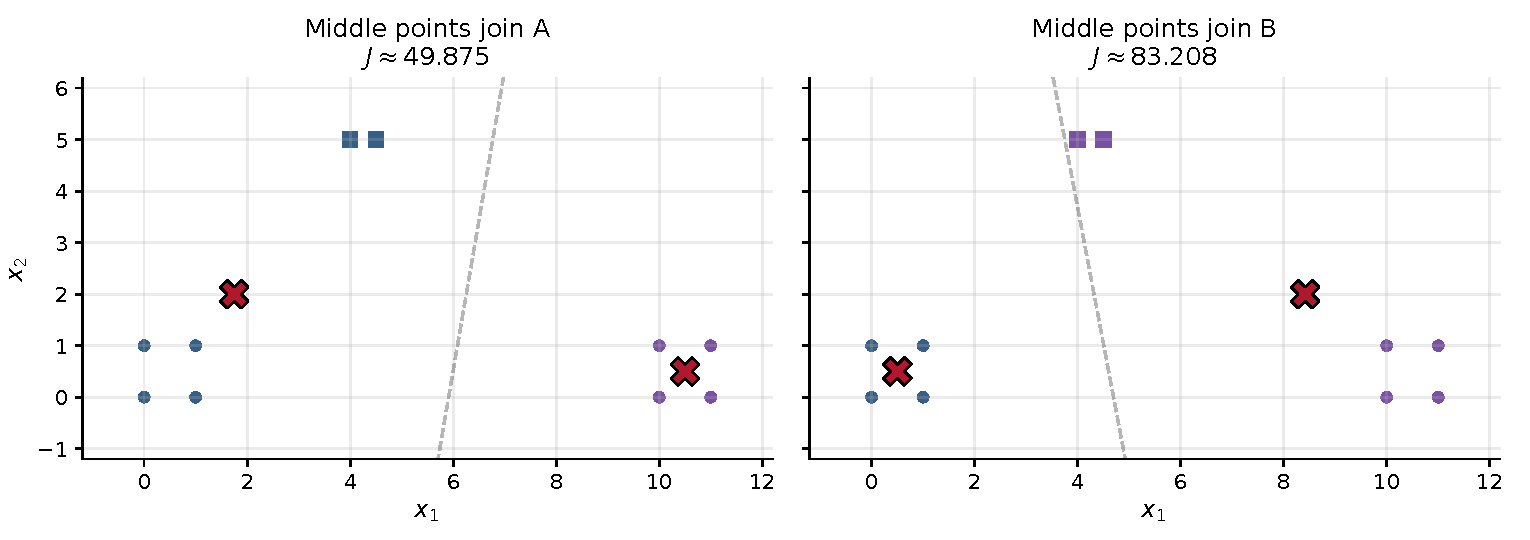
\includegraphics[width=\textwidth]{figures/handouts/em_algorithm/fig_kmeans_fixed_points}
  \caption{A toy $k$-means instance with two stable solutions depending on how the ambiguous ``middle'' points are assigned. Even in this simple setting, the update map has multiple basins and different fixed points can have different objective values.}
  \label{fig:kmeans-fixed-points}
\end{figure}

\Cref{fig:kmeans-fixed-points} makes the basin story visible.
The central points sit near an assignment boundary.
One initialization causes them to be claimed by the left cluster; another causes them to be claimed by the right cluster.
Once those assignments differ, the cluster means move differently, which reinforces the difference on the next E-step.
The stable solutions are therefore \emph{self-consistent latent assignments}.

This is exactly why initialization is part of the method rather than an afterthought.
In latent-variable problems one rarely hopes for a global theorem of the form ``EM converges to the best optimum from everywhere.''
Instead, the practical template is
\begin{algorithm}[H]
  \caption{Two-stage template: initialization + EM refinement}
  \label{alg:two-stage-em}
  \begin{algorithmic}[1]
    \Require Model class and EM operator $M_n$, plus a cheap initializer.
    \Ensure An estimate $\hat\theta$ intended to approximate a good population maximizer.
    \State \textbf{Initialization:} produce one or more candidates $\Theta_0$ (e.g.\ moments/spectral, $k$-means++, random restarts).
    \State Pick $\theta^{(0)}\in\Theta_0$ using a simple score (e.g.\ likelihood, held-out likelihood, or a surrogate).
    \State \textbf{Refinement:} run EM iterations $\theta^{(t+1)}=M_n(\theta^{(t)})$ until convergence; return the final iterate $\hat\theta$.
  \end{algorithmic}
\end{algorithm}

The Gaussian-mixture example later keeps the same logic but replaces hard assignments by soft responsibilities.
That makes the map smooth enough to analyze with derivatives, while preserving the same basin-versus-rate distinction.

\section[Gaussian mixture]{Example II: a two-component Gaussian mixture}
\label{sec:gmm-pop-em}

We now illustrate the contractive-map picture in the simplest EM setting: a balanced two-component Gaussian mixture with known variance.
To keep notation light, we work in one dimension and parameterize the unknown mean as $\theta^\star>0$; the model is
\[
Y \sim \tfrac12\,\mathcal{N}(\theta^\star,\sigma^2) + \tfrac12\,\mathcal{N}(-\theta^\star,\sigma^2),
\]
and we estimate $\theta\in\R$.
The latent variable is the component label.
This model makes the basin picture and the local-rate picture visible in the same calculation.
The same explicit map will explain why sign determines the basin and why separation controls the slope.

\subsection{EM operator and fixed points}
\label{subsec:gmm-em-operator}

Given a sample $\{y_i\}_{i=1}^n$, EM alternates between responsibilities
$w_\theta(y_i)=\Pr(Z=+1\mid Y=y_i,\theta)$ and maximizing the resulting quadratic surrogate $Q_n(\theta'\mid\theta)$.
In this model both steps have closed forms, so the update map is one-dimensional and explicit.

\subsubsection{Deriving the EM update in closed form}
\label{subsubsec:gmm-derivation}

We parameterize the mixture using a latent label $Z\in\{-1,+1\}$ with $\Pr(Z=+1)=\Pr(Z=-1)=1/2$ and
\[
Y\mid Z=z,\theta' \sim \mathcal{N}(z\theta',\sigma^2).
\]
The complete-data log-likelihood is (up to constants)
\[
\log f_{\theta'}(y,z) = -\frac{1}{2\sigma^2}\big(y-z\theta'\big)^2.
\]
By Bayes' rule, the responsibility is
\begin{align*}
w_\theta(y)
&=\Pr(Z=+1\mid Y=y,\theta)
=\frac{\exp\!\left(-\frac{(y-\theta)^2}{2\sigma^2}\right)}{\exp\!\left(-\frac{(y-\theta)^2}{2\sigma^2}\right)+\exp\!\left(-\frac{(y+\theta)^2}{2\sigma^2}\right)} \\
&=\frac{1}{1+\exp\!\left(-\frac{(y+\theta)^2-(y-\theta)^2}{2\sigma^2}\right)}
=\frac{1}{1+\exp\!\left(-\frac{2\theta y}{\sigma^2}\right)}.
\end{align*}
Here $(y+\theta)^2-(y-\theta)^2=4\theta y$, so the responsibility is a logistic function of $\theta y/\sigma^2$.
Equivalently,
\[
2w_\theta(y)-1 = \tanh\!\left(\frac{\theta y}{\sigma^2}\right),
\]
so the ``soft label'' $2w_\theta(y)-1$ is a smooth odd function of the score $\theta y$.

The sample $Q$-function is the conditional expectation of the complete-data log-likelihood,
\[
Q_n(\theta'\mid\theta)
=
-\frac{1}{2n\sigma^2}\sum_{i=1}^n\Big(
w_\theta(y_i)\,(y_i-\theta')^2 + (1-w_\theta(y_i))\,(y_i+\theta')^2
\Big),
\]
which is a concave quadratic function of $\theta'$.
Differentiate and set the derivative equal to $0$:
\[
0
=
\frac{\partial}{\partial \theta'}Q_n(\theta'\mid\theta)
=
\frac{1}{n\sigma^2}\sum_{i=1}^n\Big(
w_\theta(y_i)\,(y_i-\theta') - (1-w_\theta(y_i))\,(y_i+\theta')
\Big).
\]
Rearrange the term inside the sum as
\[
w_\theta(y_i)\,(y_i-\theta') - (1-w_\theta(y_i))\,(y_i+\theta')
=
\big(2w_\theta(y_i)-1\big)\,y_i-\theta',
\]
so the first-order condition becomes $0=\frac{1}{n\sigma^2}\sum_{i=1}^n\big(\big(2w_\theta(y_i)-1\big)\,y_i-\theta'\big)$.
Solving for $\theta'$ yields the closed-form M-step
\[
M_n(\theta)
=
\frac{1}{n}\sum_{i=1}^n \big(2w_\theta(y_i)-1\big)\,y_i
=
\frac{1}{n}\sum_{i=1}^n y_i\,\tanh\!\left(\frac{\theta y_i}{\sigma^2}\right).
\]
At the population level, the sample average is replaced by an expectation:
\[
M(\theta)
=
\E\!\left[\big(2w_\theta(Y)-1\big)\,Y\right]
=
\E\!\left[Y\,\tanh\!\left(\frac{\theta Y}{\sigma^2}\right)\right],
\]
yielding a deterministic update map $\theta^{t+1}=M(\theta^t)$.
This formula makes the geometry visible.
The score $\theta Y$ determines the posterior sign of the latent label, and the hyperbolic tangent turns that score into a soft label in $[-1,1]$.
When the mixture components are well separated, most draws of $Y$ make $\theta Y/\sigma^2$ large in magnitude, so the soft labels are close to $\pm 1$ and EM behaves almost like a hard assignment step.
When the components are weakly separated, the same soft labels stay closer to $0$, so the map lies nearer the diagonal and refinement is slower.

\begin{lemma}[Population fixed points for the symmetric mixture]
\label{lem:gmm-fixed-points}
Under the population model $Y=Z\theta^\star+\varepsilon$ with $Z\in\{-1,+1\}$ uniform and $\varepsilon\sim \mathcal{N}(0,\sigma^2)$ independent of $Z$, the population EM map satisfies
\[
M(\theta^\star)=\theta^\star,
\qquad
M(-\theta^\star)=-\theta^\star,
\qquad
M(0)=0.
\]
\end{lemma}

\begin{proof}
For any $\theta$, the posterior mean of the label is
\[
\E[Z\mid Y=y,\theta]
= (+1)\Pr(Z=+1\mid y,\theta) + (-1)\Pr(Z=-1\mid y,\theta)
=2w_\theta(y)-1.
\]
Therefore $M(\theta)=\E\!\left[Y\,\E[Z\mid Y,\theta]\right]$.
At $\theta=\theta^\star$, the conditional expectation is taken under the true model, so by the tower property
\[
M(\theta^\star)
=\E\!\left[Y\,\E[Z\mid Y,\theta^\star]\right]
=\E[YZ].
\]
Since $Y=Z\theta^\star+\varepsilon$ with $\varepsilon\perp Z$ and $Z^2=1$, we have $\E[YZ]=\E[(Z\theta^\star+\varepsilon)Z]=\theta^\star$.
The identity $M(-\theta^\star)=-\theta^\star$ follows by the same argument (or by symmetry of the model), and $M(0)=0$ follows because $w_0(y)=1/2$ so $2w_0(y)-1=0$.
\end{proof}

In this example the geometry assumption in \Cref{thm:em-fos-implies-contraction} is immediate:
the population objective $q(\theta')=Q(\theta'\mid\theta^\star)$ is a concave quadratic in $\theta'$ with second derivative $q''(\theta')=-1/\sigma^2$, hence it is globally $(1/\sigma^2)$-strongly concave.
The remaining step is to verify that the update map is stable in the basin of interest, which in one dimension reduces to controlling the slope $|M'(\theta)|$.

The third fixed point at $0$ plays a different role.
It is a self-consistent point in the sense that perfectly ambiguous responsibilities stay ambiguous, but it is not attractive.
The next exercise computes that instability directly.

\begin{exercise}[Instability of the zero fixed point in the Gaussian mixture map]
\label{ex:gmm-zero-unstable}
Consider the population EM map
\[
M(\theta)=\E\!\left[Y\,\tanh\!\left(\frac{\theta Y}{\sigma^2}\right)\right],
\qquad
Y=Z\theta^\star+\varepsilon,\ Z\in\{-1,+1\}\text{ uniform},\ \varepsilon\sim\mathcal{N}(0,\sigma^2).
\]
\begin{enumerate}[leftmargin=*]
  \item Show that $M$ is an odd function: $M(-\theta)=-M(\theta)$.
  \item Differentiate under the expectation to show
  \[
  M'(\theta)=\E\!\left[\frac{Y^2}{\sigma^2}\cdot \frac{1}{\cosh^2\!\left(\frac{\theta Y}{\sigma^2}\right)}\right].
  \]
  \item Compute $M'(0)$ and conclude that $0$ is a locally unstable fixed point (i.e.\ $|M'(0)|>1$).
\end{enumerate}
\end{exercise}

\SolutionBox[14]{%
\emph{Part (1).}
Using that $\tanh$ is odd,
\[
M(-\theta)
=\E\!\left[Y\,\tanh\!\left(-\frac{\theta Y}{\sigma^2}\right)\right]
=-\E\!\left[Y\,\tanh\!\left(\frac{\theta Y}{\sigma^2}\right)\right]
=-M(\theta).
\]

\emph{Part (2).}
Since $\frac{d}{du}\tanh(u)=\cosh^{-2}(u)$ and $\tanh,\cosh^{-2}$ are bounded, dominated convergence justifies differentiation under the expectation:
\[
M'(\theta)
=\E\!\left[Y\cdot \frac{Y}{\sigma^2}\cdot \frac{1}{\cosh^2\!\left(\frac{\theta Y}{\sigma^2}\right)}\right]
=\E\!\left[\frac{Y^2}{\sigma^2}\cdot \frac{1}{\cosh^2\!\left(\frac{\theta Y}{\sigma^2}\right)}\right].
\]

\emph{Part (3).}
At $\theta=0$, $\cosh^2(0)=1$, so $M'(0)=\E[Y^2]/\sigma^2$.
Under $Y=Z\theta^\star+\varepsilon$ with $Z^2=1$ and $\varepsilon\perp Z$,
\[
\E[Y^2]=\E[(Z\theta^\star+\varepsilon)^2]=(\theta^\star)^2+\sigma^2,
\]
so
\[
M'(0)=\frac{(\theta^\star)^2+\sigma^2}{\sigma^2}=1+\left(\frac{\theta^\star}{\sigma}\right)^2>1.
\]
Hence $0$ is a locally unstable fixed point.%
}

\Cref{fig:em-operator-fixed-points} now has a precise interpretation:
the graph shown there is exactly the map derived above.
The fixed points are its intersections with the diagonal.
Because the model is symmetric, the population log-likelihood has two equivalent maximizers $\pm\theta^\star$, and the sign of the initialization determines which one the iterates approach.
Here that nonconvexity is benign: the two limits differ only by label swapping, so they represent the same fitted mixture distribution.
Larger separation does not change the basin picture; it changes the rate of refinement within each basin.

\subsubsection{Global convergence of population EM in one dimension}
\label{subsubsec:gmm-global-population}

\Cref{fig:em-operator-fixed-points} suggests something stronger than local contraction near $\pm\theta^\star$: in one dimension, every initialization with the correct sign appears to converge to the corresponding population maximizer.
This is true, and it is a rare example where population EM admits a clean global guarantee.

To connect this claim with the literature, write the update map as a two-argument function.
For any $m>0$, let
\[
Y_m \sim \tfrac12\,\mathcal{N}(m,\sigma^2) + \tfrac12\,\mathcal{N}(-m,\sigma^2),
\qquad
M(\theta; m)\coloneqq \E\!\left[Y_m\,\tanh\!\left(\frac{\theta Y_m}{\sigma^2}\right)\right].
\]
Our population EM map is $\theta\mapsto M(\theta;\theta^\star)$, and (by the fixed point lemma) $M(m;m)=m$.

\begin{proposition}[Sign determines the basin in the 1D symmetric mixture]
\label{prop:gmm-global-population-sign-basin}
Assume $\theta^\star>0$.
Let $\theta^{(t+1)}=M(\theta^{(t)};\theta^\star)$ be the population EM iterates.
If $\theta^{(0)}>0$, then $\theta^{(t)}>0$ for all $t$ and $\theta^{(t)}\to \theta^\star$.
By symmetry, if $\theta^{(0)}<0$ then $\theta^{(t)}\to -\theta^\star$, and if $\theta^{(0)}=0$ then $\theta^{(t)}=0$ for all $t$.
\end{proposition}

\begin{proof}
If $\theta>0$, then $y\tanh(\theta y/\sigma^2)\ge 0$ for every $y$, with strict inequality for every $y\neq 0$.
Hence $M(\theta;\theta^\star)>0$, so positive initializations remain positive under the iteration.
The convergence claims are then exactly the one-dimensional specialization of \citet[Thms.~1--2]{xu_hsu_maleki_2016_global_em}: in one dimension, the sign condition $\ip{\theta^{(0)}}{\theta^\star}\gtrless 0$ reduces to $\theta^{(0)}\gtrless 0$, so the cited theorem says the population iterates converge to the corresponding signed maximizer, while the zero initialization remains at the unstable fixed point $0$.
\end{proof}

The same reference proves the higher-dimensional analogue, where the basin is determined by the sign of the inner product $\ip{\theta^{(0)}}{\theta^\star}$ rather than by the sign of a scalar initialization; see \citet[Thms.~1--2]{xu_hsu_maleki_2016_global_em}.

In one dimension, local contractivity near a fixed point is captured by the slope $|M'(\theta^\star)|$: smaller slope means faster refinement.
Since $M(\theta)=\E\!\left[Y\tanh\!\left(\frac{\theta Y}{\sigma^2}\right)\right]$ and $\frac{d}{du}\tanh(u)=\frac{1}{\cosh^2(u)}$, we can differentiate under the expectation to get
\[
M'(\theta)
=
\E\!\left[\frac{Y^2}{\sigma^2}\cdot \frac{1}{\cosh^2\!\left(\frac{\theta Y}{\sigma^2}\right)}\right].
\]
\Cref{fig:em-contraction-vs-snr} plots this slope as a function of the signal-to-noise ratio $\theta^\star/\sigma$ for the Gaussian mixture.
Separation plays the role of a \emph{conditioning parameter} for EM: when $\theta^\star/\sigma$ is large, responsibilities are close to $0$--$1$ under the true model and the map is strongly contractive, so refinement is fast; when $\theta^\star/\sigma$ is small, responsibilities stay near $1/2$ and the slope approaches $1$, so linear convergence becomes extremely slow.
Importantly, this ``slow EM'' regime is not a mysterious algorithmic failure---it reflects the fact that the statistical model itself becomes less distinctive as $\theta^\star/\sigma\to 0$:
the mixture distribution approaches a single Gaussian, so many parameter values yield almost the same observed-data likelihood and there is little signal for any method to exploit.
In other words, low separation is often ``easy'' in a \emph{model-fit} sense (many parameter values fit about equally well), but ``hard'' in a \emph{parameter-estimation} sense (it is difficult to reliably recover the tiny component separation).

\begin{lemma}[A simple sufficient condition for local contractivity]
\label{lem:gmm-contractive-region}
For any $\theta\neq 0$, the derivative satisfies
\[
0< M'(\theta) \le \frac{4e^{-2}\sigma^2}{\theta^2}.
\]
In particular, if $\theta^\star \ge \frac{4\sigma}{e}$, then $M$ is a contraction on the interval $\big[\frac{\theta^\star}{2},\frac{3\theta^\star}{2}\big]$ with contraction factor
\[
\kappa \le \frac{16e^{-2}\sigma^2}{(\theta^\star)^2} < 1.
\]
\end{lemma}

\clearpage
\begin{exercise}[Proving \Cref{lem:gmm-contractive-region}]
\label{ex:gmm-contractive-region}
Prove \Cref{lem:gmm-contractive-region}.
\emph{Hint:} start from $M'(\theta)=\E\!\left[\frac{Y^2}{\sigma^2}\cosh^{-2}\!\left(\frac{\theta Y}{\sigma^2}\right)\right]$,
use $\cosh(u)\ge \tfrac12 e^{|u|}$, and then maximize $y^2e^{-by}$ over $y\ge 0$ for $b>0$.
\end{exercise}

\SolutionBox[22]{%
Starting from
\[
M'(\theta)
=
\E\!\left[\frac{Y^2}{\sigma^2}\cdot \frac{1}{\cosh^2\!\left(\frac{\theta Y}{\sigma^2}\right)}\right],
\]
use $\cosh(u)\ge \tfrac12 e^{|u|}$ to obtain $\cosh^{-2}(u)\le 4e^{-2|u|}$.
Hence,
\[
M'(\theta)
\le
\frac{4}{\sigma^2}\E\!\left[Y^2\exp\!\left(-\frac{2|\theta|\,|Y|}{\sigma^2}\right)\right].
\]
Fix $b>0$.  For $y\ge 0$, the function $y\mapsto y^2e^{-by}$ has derivative $e^{-by}(2y-by^2)$, so it is maximized at $y=2/b$ with value $4e^{-2}/b^2$.
Therefore $Y^2e^{-b|Y|}\le 4e^{-2}/b^2$ almost surely, and with $b=\frac{2|\theta|}{\sigma^2}$ we get
\[
M'(\theta)
\le
\frac{4}{\sigma^2}\cdot \frac{4e^{-2}}{b^2}
=
\frac{4e^{-2}\sigma^2}{\theta^2}.
\]
If $\theta^\star\ge \frac{4\sigma}{e}$ and $\theta\in[\theta^\star/2,3\theta^\star/2]$, then $|\theta|\ge \theta^\star/2$ and the bound gives
\[
\sup_{\theta\in[\theta^\star/2,3\theta^\star/2]} M'(\theta)
\le
\frac{16e^{-2}\sigma^2}{(\theta^\star)^2}
<1,
\]
so $M$ is a contraction on this interval with contraction factor $\kappa\le 16e^{-2}\sigma^2/(\theta^\star)^2$.%
}

\begin{figure}[t]
  \centering
  \begin{tikzpicture}
  \begin{axis}[
    width=0.78\linewidth,
    height=5.8cm,
    xmin=0, xmax=3,
    ymin=0, ymax=1.02,
    axis lines=left,
    xlabel={$\theta^\star/\sigma$},
    ylabel={local slope $|M'(\theta^\star)|$},
    title={Gaussian mixture: contractivity strengthens with separation},
    title style={font=\small, yshift=-0.35em},
    clip=false,
  ]
    \addplot[stat221Blue,thick] table[row sep=\\] {
x y \\
0.000000 1 \\
0.020000 0.999200639318 \\
0.040000 0.996810196552 \\
0.060000 0.99285134851 \\
0.080000 0.987361104747 \\
0.100000 0.980389691245 \\
0.120000 0.971999101273 \\
0.140000 0.962261408213 \\
0.160000 0.951256940118 \\
0.180000 0.939072410763 \\
0.200000 0.925799089615 \\
0.220000 0.911531076495 \\
0.240000 0.896363728474 \\
0.260000 0.880392269087 \\
0.280000 0.863710594595 \\
0.300000 0.846410279611 \\
0.320000 0.828579775021 \\
0.340000 0.810303784702 \\
0.360000 0.791662803511 \\
0.380000 0.772732797077 \\
0.400000 0.753585003412 \\
0.420000 0.734285836967 \\
0.440000 0.714896877044 \\
0.460000 0.695474924141 \\
0.480000 0.676072109754 \\
0.500000 0.656736047028 \\
0.520000 0.637510011546 \\
0.540000 0.618433143276 \\
0.560000 0.599540662238 \\
0.580000 0.580864091861 \\
0.600000 0.562431485194 \\
0.620000 0.544267650154 \\
0.640000 0.526394370884 \\
0.660000 0.50883062299 \\
0.680000 0.491592781046 \\
0.700000 0.474694817242 \\
0.720000 0.45814849041 \\
0.740000 0.44196352504 \\
0.760000 0.426147780064 \\
0.780000 0.41070740746 \\
0.800000 0.395647000799 \\
0.820000 0.380969734022 \\
0.840000 0.36667749078 \\
0.860000 0.352770984743 \\
0.880000 0.339249871297 \\
0.900000 0.326112851098 \\
0.920000 0.313357765928 \\
0.940000 0.300981687329 \\
0.960000 0.288980998447 \\
0.980000 0.277351469548 \\
1.000000 0.266088327605 \\
1.020000 0.255186320385 \\
1.040000 0.244639775404 \\
1.060000 0.234442654114 \\
1.080000 0.224588601677 \\
1.100000 0.215070992637 \\
1.120000 0.205882972786 \\
1.140000 0.197017497522 \\
1.160000 0.188467366949 \\
1.180000 0.180225257954 \\
1.200000 0.17228375351 \\
1.220000 0.164635369393 \\
1.240000 0.157272578521 \\
1.260000 0.150187833083 \\
1.280000 0.143373584641 \\
1.300000 0.136822302343 \\
1.320000 0.130526489398 \\
1.340000 0.124478697942 \\
1.360000 0.118671542426 \\
1.380000 0.11309771162 \\
1.400000 0.107749979356 \\
1.420000 0.102621214102 \\
1.440000 0.097704387443 \\
1.460000 0.0929925815757 \\
1.480000 0.0884789958711 \\
1.500000 0.0841569525892 \\
1.520000 0.0800199018077 \\
1.540000 0.0760614256251 \\
1.560000 0.0722752416963 \\
1.580000 0.0686552061522 \\
1.600000 0.0651953159532 \\
1.620000 0.0618897107203 \\
1.640000 0.0587326740874 \\
1.660000 0.0557186346124 \\
1.680000 0.052842166284 \\
1.700000 0.0500979886587 \\
1.720000 0.0474809666585 \\
1.740000 0.044986110062 \\
1.760000 0.0426085727134 \\
1.780000 0.0403436514783 \\
1.800000 0.0381867849676 \\
1.820000 0.0361335520504 \\
1.840000 0.0341796701761 \\
1.860000 0.0323209935227 \\
1.880000 0.0305535109896 \\
1.900000 0.0288733440535 \\
1.920000 0.027276744506 \\
1.940000 0.0257600920913 \\
1.960000 0.0243198920608 \\
1.980000 0.0229527726556 \\
2.000000 0.0216554825256 \\
2.020000 0.0204248880892 \\
2.040000 0.019257970835 \\
2.060000 0.0181518245719 \\
2.080000 0.017103652636 \\
2.100000 0.0161107650723 \\
2.120000 0.0151705758106 \\
2.140000 0.0142805998594 \\
2.160000 0.0134384505301 \\
2.180000 0.0126418366964 \\
2.200000 0.0118885600784 \\
2.220000 0.0111765125314 \\
2.240000 0.0105036733215 \\
2.260000 0.00986810637488 \\
2.280000 0.00926795751283 \\
2.300000 0.00870145169878 \\
2.320000 0.00816689034165 \\
2.340000 0.00766264869717 \\
2.360000 0.00718717339248 \\
2.380000 0.00673898006967 \\
2.400000 0.00631665111137 \\
2.420000 0.00591883339061 \\
2.440000 0.0055442359866 \\
2.460000 0.00519162783269 \\
2.480000 0.00485983530513 \\
2.500000 0.00454773980721 \\
2.520000 0.00425427543351 \\
2.540000 0.00397842680007 \\
2.560000 0.00371922709277 \\
2.580000 0.00347575632804 \\
2.600000 0.00324713975739 \\
2.620000 0.00303254630428 \\
2.640000 0.00283118691814 \\
2.660000 0.00264231277163 \\
2.680000 0.00246521330105 \\
2.700000 0.00229921417106 \\
2.720000 0.00214367530193 \\
2.740000 0.001997989106 \\
2.760000 0.00186157903248 \\
2.780000 0.00173389843058 \\
2.800000 0.00161442964015 \\
2.820000 0.00150268314598 \\
2.840000 0.00139819661532 \\
2.860000 0.00130053368832 \\
2.880000 0.00120928249346 \\
2.900000 0.00112405397779 \\
2.920000 0.00104448023229 \\
2.940000 0.000970213019799 \\
2.960000 0.000900922663713 \\
2.980000 0.00083629734512 \\
3.000000 0.000776042723369 \\
    };

    \addplot[only marks,mark=*,mark size=1.3pt,stat221Orange] coordinates {
      (0.600000,0.562431485194)
      (2.000000,0.0216554825256)
    };
    \node[font=\small,anchor=south east] at (axis cs:0.600000,0.562431485194) {0.6};
    \node[font=\small,anchor=south west] at (axis cs:2.000000,0.0216554825256) {2};
  \end{axis}
\end{tikzpicture}

  \caption{Local contraction factor $|M'(\theta^\star)|$ for population EM in the symmetric two-component Gaussian mixture, as a function of the signal-to-noise ratio $\theta^\star/\sigma$. Larger separation leads to much stronger contractivity near the population maximizer, hence faster refinement once initialized in the correct basin.}
  \label{fig:em-contraction-vs-snr}
\end{figure}

\subsection{Local theory near a good fixed point}
\label{subsec:em-population-contractivity-template}

The Gaussian-mixture example already contains the shape of a general EM theorem.
Likelihood ascent is only part of the story.
It says that EM does not decrease the observed-data likelihood, but it does not say whether the initialization lies in the basin of a desirable fixed point, whether the population map pulls the iterates back once they are near that point, or whether finite-sample noise distorts that picture.
That is why useful EM results are usually local.

To study the local behavior near a good population fixed point $\theta^\star$, freeze the second argument of the surrogate at $\theta^\star$ and define
\[
q(\theta') \coloneqq Q(\theta' \mid \theta^\star).
\]
This is the surrogate EM would maximize if the E-step already used the correct posterior law.
From that viewpoint, the local theory is built out of two ideas.
First, the ideal objective $q$ should have enough curvature near $\theta^\star$ that maximizing it would correct small perturbations away from the target.
Second, the E-step should be stable: replacing $\theta^\star$ by a nearby iterate $\theta$ should not change the surrogate gradient too much.
If both statements hold, then the true EM map behaves like a perturbed maximization of $q$, so one can prove contraction for the population map and then transfer that result to the sample map by a perturbation argument.
The next definitions write those two ideas in a form suitable for the proof.

\begin{definition}[Local strong concavity]
\label{def:em-local-strong-concavity}
Fix $r>0$ and define the ball $B_r(\theta^\star)\coloneqq\{\theta\in\Theta:\norm{\theta-\theta^\star}_2\le r\}$.
We say $q$ is \textbf{$\lambda$-strongly concave on $B_r(\theta^\star)$} if for all $\theta_1,\theta_2\in B_r(\theta^\star)$,
\[
q(\theta_1)
\le
q(\theta_2)
\;+\;
\ip{\nabla q(\theta_2)}{\theta_1-\theta_2}
\;-\;
\frac{\lambda}{2}\norm{\theta_1-\theta_2}_2^2.
\]
\end{definition}

\begin{definition}[First-order stability (FOS)]
\label{def:em-fos}
Fix $r>0$.
We say the population $Q$-functions satisfy \textbf{$\mathrm{FOS}(\gamma)$ on $B_r(\theta^\star)$} if for all $\theta\in B_r(\theta^\star)$,
\[
\norm{\nabla_{\theta'} Q(M(\theta)\mid \theta^\star)-\nabla_{\theta'} Q(M(\theta)\mid \theta)}_2
\le
\gamma \norm{\theta-\theta^\star}_2.
\]
\end{definition}

\begin{theorem}[FOS + strong concavity $\Rightarrow$ contraction of population EM]
\label{thm:em-fos-implies-contraction}
Fix $r>0$ and define $B_r(\theta^\star)$ as in \Cref{def:em-local-strong-concavity}.
Assume:
\begin{enumerate}[leftmargin=*]
  \item $\theta^\star$ is self-consistent, meaning $M(\theta^\star)=\theta^\star$.
  \item $q(\cdot)=Q(\cdot\mid\theta^\star)$ is $\lambda$-strongly concave on $B_r(\theta^\star)$.
  \item $\mathrm{FOS}(\gamma)$ holds on $B_r(\theta^\star)$ for some $\gamma\in[0,\lambda)$.
  \item For all $\theta\in B_r(\theta^\star)$, the update $M(\theta)$ also lies in $B_r(\theta^\star)$.
  \item $\theta^\star$ is an interior maximizer of $q$, and for each $\theta\in B_r(\theta^\star)$ the EM update $M(\theta)$ is an interior maximizer of $\theta'\mapsto Q(\theta'\mid\theta)$, so that
  \[
  \nabla q(\theta^\star)=0,
  \qquad
  \nabla_{\theta'} Q(M(\theta)\mid\theta)=0.
  \]
\end{enumerate}
Then $M$ is contractive on $B_r(\theta^\star)$ with contraction factor $\kappa=\gamma/\lambda$:
\[
\norm{M(\theta)-\theta^\star}_2
\le
\frac{\gamma}{\lambda}\norm{\theta-\theta^\star}_2
\qquad\text{for all }\theta\in B_r(\theta^\star).
\]
\end{theorem}

\begin{proof}
Fix $\theta\in B_r(\theta^\star)$ and write $\bar\theta \coloneqq M(\theta)$.
By local invariance, $\bar\theta\in B_r(\theta^\star)$.
By \Cref{def:em-local-strong-concavity}, the function $-q$ is $\lambda$-strongly convex on $B_r(\theta^\star)$, so for all $u,v\in B_r(\theta^\star)$,
\[
\ip{\nabla q(u)-\nabla q(v)}{u-v}
\le
-\lambda\norm{u-v}_2^2,
\]
and therefore, by Cauchy--Schwarz,
\[
\lambda\norm{u-v}_2
\le
\norm{\nabla q(u)-\nabla q(v)}_2.
\]
Apply this with $u=\bar\theta$ and $v=\theta^\star$, and use $\nabla q(\theta^\star)=0$, to obtain
\[
\lambda\norm{\bar\theta-\theta^\star}_2
\le
\norm{\nabla q(\bar\theta)}_2
=
\norm{\nabla_{\theta'} Q(\bar\theta\mid\theta^\star)}_2.
\]
By the interior optimality condition $\nabla_{\theta'} Q(\bar\theta\mid\theta)=0$ and $\mathrm{FOS}(\gamma)$,
\[
\norm{\nabla_{\theta'} Q(\bar\theta\mid\theta^\star)}_2
=
\norm{\nabla_{\theta'} Q(\bar\theta\mid\theta^\star)-\nabla_{\theta'} Q(\bar\theta\mid\theta)}_2
\le
\gamma\norm{\theta-\theta^\star}_2.
\]
Combine the last two displays and divide by $\lambda$.
\end{proof}

In words, strong concavity tells us that the ideal M-step would correct deviations from $\theta^\star$, while FOS says the real E-step does not distort that ideal picture too much.
If FOS fails badly, then changing the current iterate can change the posterior weights so much that the update map loses its restorative pull.

\subsubsection{Gradient EM: an inexact M-step}
\label{subsec:em-gradient-em}

In large models, the exact maximization step defining $M(\theta)$ can be expensive.
A common alternative is to take one gradient ascent step on the surrogate $Q(\cdot\mid\theta)$ starting from $\theta$.
At the population level, this defines the \emph{gradient EM} operator
\[
G(\theta)\coloneqq \theta + \alpha\,\nabla_{\theta'} Q(\theta\mid\theta),
\]
where $\alpha>0$ is a step size.
(The sample version replaces $Q$ by $Q_n$.)

If we could take gradient ascent on the ideal objective $q(\theta)=Q(\theta\mid\theta^\star)$ directly, then strong concavity and smoothness would give a contraction for an appropriate step size; see \citep[\S9.2]{boyd_vandenberghe_2004_convex}.
Gradient EM behaves similarly when the surrogate gradient is stable near $\theta^\star$.

\begin{definition}[Gradient stability (GS)]
\label{def:em-gs}
Fix $r>0$.
We say the population $Q$-functions satisfy \textbf{$\mathrm{GS}(\gamma)$ on $B_r(\theta^\star)$} if for all $\theta\in B_r(\theta^\star)$,
\[
\norm{\nabla_{\theta'} Q(\theta\mid \theta^\star)-\nabla_{\theta'} Q(\theta\mid \theta)}_2
\le
\gamma \norm{\theta-\theta^\star}_2.
\]
\end{definition}

\begin{theorem}[GS + strong concavity $\Rightarrow$ contraction of gradient EM]
\label{thm:em-gs-implies-contraction}
Fix $r>0$ and assume:
\begin{enumerate}[leftmargin=*]
  \item $q(\cdot)=Q(\cdot\mid\theta^\star)$ is $\lambda$-strongly concave and $L$-smooth on $B_r(\theta^\star)$, with $0<\lambda\le L$.
  \item $\mathrm{GS}(\gamma)$ holds on $B_r(\theta^\star)$ for some $\gamma\in[0,\lambda)$.
  \item $\theta^\star$ is an interior maximizer of $q$, so $\nabla q(\theta^\star)=0$.
\end{enumerate}
Then gradient EM with step size $\alpha=\frac{2}{L+\lambda}$ is contractive on $B_r(\theta^\star)$:
\[
\norm{G(\theta)-\theta^\star}_2
\le
\left(\frac{L-\lambda+2\gamma}{L+\lambda}\right)\norm{\theta-\theta^\star}_2
\qquad\text{for all }\theta\in B_r(\theta^\star).
\]
\end{theorem}

\begin{proof}
Write $G(\theta)-\theta^\star$ as
\[
\underbrace{\theta + \alpha \nabla q(\theta)-\theta^\star}_{\text{gradient ascent on $q$}}
\;+\;
\alpha\underbrace{\bigl(\nabla_{\theta'} Q(\theta\mid\theta)-\nabla_{\theta'} Q(\theta\mid\theta^\star)\bigr)}_{\text{stability error}}.
\]
For $\alpha=\frac{2}{L+\lambda}$, gradient ascent on a $\lambda$-strongly concave, $L$-smooth function is a contraction mapping with factor $\frac{L-\lambda}{L+\lambda}$ (equivalently, apply the standard strongly convex result to $-q$).
Combine this with \Cref{def:em-gs} and $\alpha=\frac{2}{L+\lambda}$ to get
\[
\norm{G(\theta)-\theta^\star}_2
\le
\left(\frac{L-\lambda}{L+\lambda} + \frac{2\gamma}{L+\lambda}\right)\norm{\theta-\theta^\star}_2,
\]
which is the claim.
\end{proof}

Once a population contraction factor is available for either exact EM or gradient EM, the sample-level picture follows from a perturbation argument.

\begin{lemma}[Contraction + perturbation $\Rightarrow$ convergence to a neighborhood]
\label{lem:contraction-perturbation}
Fix a point $\theta^\star\in\Theta$ and a radius $r>0$.
Assume:
\begin{enumerate}[leftmargin=*]
  \item $M(\theta^\star)=\theta^\star$ and, for all $\theta$ with $\norm{\theta-\theta^\star}_2\le r$,
  \[
  \norm{M(\theta)-\theta^\star}_2 \le \kappa \norm{\theta-\theta^\star}_2
  \quad\text{for some }\kappa\in(0,1).
  \]
  \item For all $\theta$ with $\norm{\theta-\theta^\star}_2\le r$,
  \[
  \norm{M_n(\theta)-M(\theta)}_2 \le \varepsilon_n.
  \]
\end{enumerate}
Then any iterate sequence $\theta^{t+1}=M_n(\theta^t)$ that remains in the ball satisfies
\[
\norm{\theta^t-\theta^\star}_2
\le
\kappa^t \norm{\theta^0-\theta^\star}_2 + \frac{\varepsilon_n}{1-\kappa}.
\]
\end{lemma}

\begin{proof}
Write
\[
\norm{\theta^{t+1}-\theta^\star}_2
\le
\norm{M(\theta^t)-\theta^\star}_2 + \norm{M_n(\theta^t)-M(\theta^t)}_2
\le
\kappa\norm{\theta^t-\theta^\star}_2 + \varepsilon_n,
\]
then unroll the recursion.
\end{proof}

\Cref{lem:contraction-perturbation} is the core population-to-sample message.
Inside a basin where the sample map stays uniformly close to the population map, optimization error decays geometrically until it reaches a floor of order $\varepsilon_n/(1-\kappa)$.
Equivalently, sample EM converges to the sample fixed point in its basin, while the gap between that sample target and the population target is the residual statistical error.

\subsection{Finite-sample EM: geometric decay until a floor}
\label{sec:finite-sample-floor}

At finite $n$, the operator $M_n$ fluctuates around $M$.
In a neighborhood where $M$ is contractive and $M_n$ is uniformly close to $M$, \Cref{lem:contraction-perturbation} gives geometric decay until the remaining error is on the order of $1/\sqrt{n}$.

\begin{figure}[t]
  \centering
  \begin{tikzpicture}
  \begin{axis}[
    width=0.92\linewidth,
    height=6.2cm,
    xmin=0, xmax=22,
    ymode=log,
    axis lines=left,
    xlabel={EM iteration $t$},
    ylabel={distance $|\theta^{(t)}-\theta^\star|$},
    title={Gaussian mixture: geometric refinement until a sample-size floor},
    title style={font=\small, yshift=-0.35em},
    legend style={draw=stat221Gray!25, fill=white, fill opacity=0.95, text opacity=1},
    legend pos=north east,
    clip=false,
  ]
    \addplot[stat221Gray,thick,densely dashed] table[row sep=\\] {
x y \\
0.000000 1.8 \\
1.000000 1.09729288275 \\
2.000000 0.109028376417 \\
3.000000 0.00261865712788 \\
4.000000 5.68444330535e-05 \\
5.000000 1.23073156089e-06 \\
6.000000 2.63256854094e-08 \\
7.000000 2.43660647214e-10 \\
8.000000 3.21158211136e-10 \\
9.000000 3.33389760243e-10 \\
10.000000 3.33654437412e-10 \\
11.000000 3.33660210572e-10 \\
12.000000 3.33660654661e-10 \\
13.000000 3.33660654661e-10 \\
14.000000 3.33660654661e-10 \\
15.000000 3.33660654661e-10 \\
16.000000 3.33660654661e-10 \\
17.000000 3.33660654661e-10 \\
18.000000 3.33660654661e-10 \\
19.000000 3.33660654661e-10 \\
20.000000 3.33660654661e-10 \\
21.000000 3.33660654661e-10 \\
22.000000 3.33660654661e-10 \\
    };
    \addlegendentry{Population EM}

    % n=250
    \addplot[stat221Red,thick] table[row sep=\\] {
x y \\
0.000000 1.8 \\
1.000000 1.09872386901 \\
2.000000 0.110299246121 \\
3.000000 0.0505039018034 \\
4.000000 0.0515472428277 \\
5.000000 0.0515163642603 \\
6.000000 0.0515154249441 \\
7.000000 0.0515153981012 \\
8.000000 0.0515153973593 \\
9.000000 0.0515153973392 \\
10.000000 0.0515153973386 \\
11.000000 0.0515153973386 \\
12.000000 0.0515153973386 \\
13.000000 0.0515153973386 \\
14.000000 0.0515153973386 \\
15.000000 0.0515153973386 \\
16.000000 0.0515153973386 \\
17.000000 0.0515153973386 \\
18.000000 0.0515153973386 \\
19.000000 0.0515153973386 \\
20.000000 0.0515153973386 \\
21.000000 0.0515153973386 \\
22.000000 0.0515153973386 \\
    };
    \addlegendentry{$n=250$ (median)}
    \addplot[stat221Red!50,thin] table[row sep=\\] {
x y \\
0.000000 1.8 \\
1.000000 1.06088484132 \\
2.000000 0.0558003250334 \\
3.000000 0.0172269337719 \\
4.000000 0.0187376939554 \\
5.000000 0.0186938843451 \\
6.000000 0.0186928789526 \\
7.000000 0.0186928558916 \\
8.000000 0.0186928553628 \\
9.000000 0.0186928553507 \\
10.000000 0.0186928553504 \\
11.000000 0.0186928553504 \\
12.000000 0.0186928553504 \\
13.000000 0.0186928553504 \\
14.000000 0.0186928553504 \\
15.000000 0.0186928553504 \\
16.000000 0.0186928553504 \\
17.000000 0.0186928553504 \\
18.000000 0.0186928553504 \\
19.000000 0.0186928553504 \\
20.000000 0.0186928553504 \\
21.000000 0.0186928553504 \\
22.000000 0.0186928553504 \\
    };
    \addplot[stat221Red!50,thin] table[row sep=\\] {
x y \\
0.000000 1.8 \\
1.000000 1.13749626527 \\
2.000000 0.195839244443 \\
3.000000 0.110853135634 \\
4.000000 0.10599630166 \\
5.000000 0.105840011233 \\
6.000000 0.105834999751 \\
7.000000 0.105834838944 \\
8.000000 0.10583483378 \\
9.000000 0.105834833614 \\
10.000000 0.105834833609 \\
11.000000 0.105834833608 \\
12.000000 0.105834833608 \\
13.000000 0.105834833608 \\
14.000000 0.105834833608 \\
15.000000 0.105834833608 \\
16.000000 0.105834833608 \\
17.000000 0.105834833608 \\
18.000000 0.105834833608 \\
19.000000 0.105834833608 \\
20.000000 0.105834833608 \\
21.000000 0.105834833608 \\
22.000000 0.105834833608 \\
    };

    % n=1000
    \addplot[stat221Purple,thick] table[row sep=\\] {
x y \\
0.000000 1.8 \\
1.000000 1.0983030735 \\
2.000000 0.116403226832 \\
3.000000 0.0249846970799 \\
4.000000 0.0271994451237 \\
5.000000 0.0272440273864 \\
6.000000 0.027244923102 \\
7.000000 0.0272449411 \\
8.000000 0.0272449414617 \\
9.000000 0.027244941469 \\
10.000000 0.0272449414691 \\
11.000000 0.0272449414691 \\
12.000000 0.0272449414691 \\
13.000000 0.0272449414691 \\
14.000000 0.0272449414691 \\
15.000000 0.0272449414691 \\
16.000000 0.0272449414691 \\
17.000000 0.0272449414691 \\
18.000000 0.0272449414691 \\
19.000000 0.0272449414691 \\
20.000000 0.0272449414691 \\
21.000000 0.0272449414691 \\
22.000000 0.0272449414691 \\
    };
    \addlegendentry{$n=1000$ (median)}
    \addplot[stat221Purple!55,thin] table[row sep=\\] {
x y \\
0.000000 1.8 \\
1.000000 1.08333007975 \\
2.000000 0.0836193134053 \\
3.000000 0.0103829014241 \\
4.000000 0.00847228156732 \\
5.000000 0.00841108953049 \\
6.000000 0.00840974432263 \\
7.000000 0.00840971474938 \\
8.000000 0.00840971409918 \\
9.000000 0.00840971408488 \\
10.000000 0.00840971408457 \\
11.000000 0.00840971408456 \\
12.000000 0.00840971408456 \\
13.000000 0.00840971408456 \\
14.000000 0.00840971408456 \\
15.000000 0.00840971408456 \\
16.000000 0.00840971408456 \\
17.000000 0.00840971408456 \\
18.000000 0.00840971408456 \\
19.000000 0.00840971408456 \\
20.000000 0.00840971408456 \\
21.000000 0.00840971408456 \\
22.000000 0.00840971408456 \\
    };
    \addplot[stat221Purple!55,thin] table[row sep=\\] {
x y \\
0.000000 1.8 \\
1.000000 1.12615938693 \\
2.000000 0.165376411295 \\
3.000000 0.0472545773638 \\
4.000000 0.0455814764069 \\
5.000000 0.0455189731835 \\
6.000000 0.0455173198223 \\
7.000000 0.0455172765315 \\
8.000000 0.0455172754058 \\
9.000000 0.0455172753767 \\
10.000000 0.0455172753759 \\
11.000000 0.0455172753759 \\
12.000000 0.0455172753759 \\
13.000000 0.0455172753759 \\
14.000000 0.0455172753759 \\
15.000000 0.0455172753759 \\
16.000000 0.0455172753759 \\
17.000000 0.0455172753759 \\
18.000000 0.0455172753759 \\
19.000000 0.0455172753759 \\
20.000000 0.0455172753759 \\
21.000000 0.0455172753759 \\
22.000000 0.0455172753759 \\
    };

    % n=4000
    \addplot[stat221Blue,thick] table[row sep=\\] {
x y \\
0.000000 1.8 \\
1.000000 1.09776860352 \\
2.000000 0.106236150851 \\
3.000000 0.0150328312308 \\
4.000000 0.0136287629058 \\
5.000000 0.0136241329475 \\
6.000000 0.0136239966889 \\
7.000000 0.0136239929464 \\
8.000000 0.0136239928479 \\
9.000000 0.0136239928454 \\
10.000000 0.0136239928454 \\
11.000000 0.0136239928454 \\
12.000000 0.0136239928454 \\
13.000000 0.0136239928454 \\
14.000000 0.0136239928454 \\
15.000000 0.0136239928454 \\
16.000000 0.0136239928454 \\
17.000000 0.0136239928454 \\
18.000000 0.0136239928454 \\
19.000000 0.0136239928454 \\
20.000000 0.0136239928454 \\
21.000000 0.0136239928454 \\
22.000000 0.0136239928454 \\
    };
    \addlegendentry{$n=4000$ (median)}
    \addplot[stat221Blue!55,thin] table[row sep=\\] {
x y \\
0.000000 1.8 \\
1.000000 1.08188882734 \\
2.000000 0.0820973327345 \\
3.000000 0.00770508259319 \\
4.000000 0.0065464756106 \\
5.000000 0.00660028365008 \\
6.000000 0.00660143725538 \\
7.000000 0.00660146199262 \\
8.000000 0.00660146252319 \\
9.000000 0.00660146253458 \\
10.000000 0.00660146253482 \\
11.000000 0.00660146253483 \\
12.000000 0.00660146253483 \\
13.000000 0.00660146253483 \\
14.000000 0.00660146253483 \\
15.000000 0.00660146253483 \\
16.000000 0.00660146253483 \\
17.000000 0.00660146253483 \\
18.000000 0.00660146253483 \\
19.000000 0.00660146253483 \\
20.000000 0.00660146253483 \\
21.000000 0.00660146253483 \\
22.000000 0.00660146253483 \\
    };
    \addplot[stat221Blue!55,thin] table[row sep=\\] {
x y \\
0.000000 1.8 \\
1.000000 1.10460440298 \\
2.000000 0.12368330304 \\
3.000000 0.022890556425 \\
4.000000 0.022627348017 \\
5.000000 0.0226500740391 \\
6.000000 0.0226504929312 \\
7.000000 0.0226505004549 \\
8.000000 0.022650500585 \\
9.000000 0.0226505005871 \\
10.000000 0.0226505005871 \\
11.000000 0.0226505005871 \\
12.000000 0.0226505005871 \\
13.000000 0.0226505005871 \\
14.000000 0.0226505005871 \\
15.000000 0.0226505005871 \\
16.000000 0.0226505005871 \\
17.000000 0.0226505005871 \\
18.000000 0.0226505005871 \\
19.000000 0.0226505005871 \\
20.000000 0.0226505005871 \\
21.000000 0.0226505005871 \\
22.000000 0.0226505005871 \\
    };
  \end{axis}
\end{tikzpicture}

  \caption{Distance to $\theta^\star$ versus EM iteration in the Gaussian mixture example. Population EM converges linearly to $\theta^\star$. Sample EM tracks the population dynamics until it reaches a sample-dependent floor.}
  \label{fig:em-pop-vs-sample}
\end{figure}

In this example, once the initialization lands in the correct basin, the population map is contractive and the sample map tracks it until the iterate reaches an $n$-dependent statistical floor.
Separation does not change which basin is correct; it changes the speed of refinement inside that basin.

A systematic development of this population-to-sample contraction argument appears in \citet[Thm.~1]{balakrishnan_wainwright_yu_2014_em}.
Moreover, this two-Gaussian mixture is one of the rare latent-variable models where much stronger \emph{global} guarantees are possible; see, e.g., \citet[Thm.~1]{xu_hsu_maleki_2016_global_em}.

\clearpage
% ------------------------------------------------------------
\section[Missing covariates]{Example III: regression with missing covariates}
\label{sec:missing-covariates}

EM is also natural outside mixture models whenever part of the data is latent or unobserved.
A basic example is linear regression with covariates missing completely at random.
Let $X\in\R^d$ and $Y\in\R$ follow the population model
\[
X \sim \mathcal{N}(0,I_d),
\qquad
Y = \ip{X}{\theta^\star} + \varepsilon,
\qquad
\varepsilon \sim \mathcal{N}(0,\sigma^2)\ \text{independent of }X,
\]
and suppose we observe $Y$ but only a subset of the coordinates of $X$.
Formally, each coordinate is missing with probability $\rho\in[0,1)$, independently across coordinates and samples.
The missing coordinates are treated as latent variables, so EM alternates between imputing them from the conditional law of $X$ given $(X_{\mathrm{obs}},Y)$ and refitting $\theta'$ by weighted least squares using the conditional moments $\E[X\mid X_{\mathrm{obs}},Y,\theta]$ and $\E[XX^\top\mid X_{\mathrm{obs}},Y,\theta]$.

This example complements the Gaussian mixture.
In the mixture model, weak separation mainly makes the EM map flatter near the correct target.
Here the more basic issue is that the E-step literally fills in unseen coordinates using the \emph{current} parameter.
If $\theta$ is already close to $\theta^\star$, those imputations are helpful.
If $\theta$ points in a badly wrong direction and the missingness level is high, the imputations can reinforce that wrong direction, so the map itself can develop a bad stable fixed point.

\subsection{Missingness and identifiability}
\label{subsec:missing-covariates-identifiability-limit}

As $\rho$ increases, fewer coordinates of $X$ are observed, the E-step becomes less informative, and both optimization and statistical estimation become harder.

The extreme case $\rho=1$ shows the identifiability issue most clearly.
If all covariates are missing, then the observed data are only the responses $\{Y_i\}_{i=1}^n$.
Because $X\sim\mathcal{N}(0,I_d)$, for any parameter $\theta$ we have $\ip{X}{\theta}\sim \mathcal{N}(0,\norm{\theta}_2^2)$, so
\[
Y \mid \theta
\sim
\mathcal{N}\!\big(0,\norm{\theta}_2^2+\sigma^2\big).
\]
Therefore the distribution of the observed data depends on $\theta$ only through $\norm{\theta}_2$.
In particular, the direction of $\theta^\star$ is \emph{not identifiable}: any $\tilde\theta$ with $\norm{\tilde\theta}_2=\norm{\theta^\star}_2$ produces the same law for $Y$.
No algorithm (EM included) can recover what the data do not contain; at best, one can hope to estimate $\norm{\theta^\star}_2$.
\Cref{fig:em-nonidentifiability-ridge} gives a schematic picture.

\begin{figure}[t]
  \centering
  \begin{tikzpicture}
  \begin{axis}[
    width=0.62\linewidth,
    height=6.0cm,
    axis lines=middle,
    xmin=-1.6, xmax=1.6,
    ymin=-1.6, ymax=1.6,
    xlabel={$\theta_1$},
    ylabel={$\theta_2$},
    xtick=\empty,
    ytick=\empty,
    clip=false,
  ]
    \addplot[stat221Blue,thick,domain=0:360,samples=200] ({cos(x)}, {sin(x)});

    \addplot[only marks,mark=*,mark size=1.2pt,stat221Red] coordinates {(1,0)};
    \node[
      font=\small,
      anchor=south west,
      fill=white,
      fill opacity=0.92,
      text opacity=1,
      inner sep=1pt,
      rounded corners=1pt,
    ] at (axis cs:1.050000,0.080000) {$\theta^\star$};

    \addplot[only marks,mark=*,mark size=1.2pt,stat221Purple] coordinates {(0,1)};
    \node[
      font=\small,
      anchor=south east,
      fill=white,
      fill opacity=0.92,
      text opacity=1,
      inner sep=1pt,
      rounded corners=1pt,
    ] at (axis cs:-0.040000,1.070000) {$\tilde\theta$};

    \node[
      font=\small,
      align=center,
      stat221Gray,
      fill=white,
      fill opacity=0.92,
      text opacity=1,
      inner sep=1.5pt,
      rounded corners=1pt,
    ] at (axis cs:0,-1.420000) {same observed law\\(same $\|\theta\|_2$)};
  \end{axis}
\end{tikzpicture}

  \caption{Non-identifiability in the ``noise-only'' limit.  When $\rho=1$, we never observe any coordinates of $X$, and the marginal law is $Y\mid\theta\sim\mathcal{N}(0,\norm{\theta}_2^2+\sigma^2)$.  Hence all parameters on a sphere $\{\theta:\norm{\theta}_2=\text{const}\}$ induce the same distribution of $Y$, so there cannot be a contraction toward a unique maximizer.}
  \label{fig:em-nonidentifiability-ridge}
\end{figure}

This illustrates a different failure mode than low separation in mixtures.
In Example II, low separation mainly means weak identification and poor conditioning: there is a well-defined population target up to the sign symmetry, but the likelihood is relatively flat and the EM contraction factor is close to $1$, so refinement is slow and statistical accuracy requires very large $n$.
Here, increasing missingness pushes the statistical problem itself toward non-identifiability, so EM no longer has a unique population target to contract toward.

\subsection{Deriving the EM operator in closed form}
\label{subsec:missing-covariates-derivation}

Because the model is Gaussian, the E-step conditional moments can be written explicitly and the M-step reduces to a linear system.
These formulas show exactly where the self-reinforcement enters:
the posterior moments used in the E-step depend on the current iterate $\theta$, so the regression problem solved by the M-step is built out of \emph{imputed} covariates that already reflect the current belief.

\subsubsection{E-step: conditional moments from a joint Gaussian}
\label{subsubsec:missing-covariates-estep}

Fix one observation $(x_{\mathrm{obs}},y)$ and let $O\subseteq\{1,\dots,d\}$ be the set of observed coordinates, with $M$ its complement.
Write the parameter and covariate vector in blocks $\theta=(\theta_M,\theta_O)$ and $X=(X_M,X_O)$.
Conditioned on $X_O=x_O$, the scalar response model under parameter $\theta$ is
\[
Y = \ip{\theta_O}{x_O} + \ip{\theta_M}{X_M} + \varepsilon,
\qquad
X_M\sim\mathcal{N}(0,I),
\qquad
\varepsilon\sim\mathcal{N}(0,\sigma^2),
\]
so $X_M\mid (X_O=x_O,Y=y,\theta)$ is the Gaussian posterior in a one-dimensional linear measurement model.
A standard conditioning calculation (e.g.\ via Sherman--Morrison) yields
\begin{align}
\label{eq:missing-covariates-posterior-mean}
\E[X_M\mid x_O,y,\theta]
&=
\frac{\theta_M}{\sigma^2+\norm{\theta_M}_2^2}\,\Big(y-\ip{\theta_O}{x_O}\Big), \\
\label{eq:missing-covariates-posterior-cov}
\mathrm{Cov}(X_M\mid x_O,y,\theta)
&=
I-\frac{\theta_M\theta_M^\top}{\sigma^2+\norm{\theta_M}_2^2}.
\end{align}

Define the conditional mean and second moment of the \emph{full} covariate vector,
\[
\mu_\theta(x_{\mathrm{obs}},y)\coloneqq \E[X\mid X_{\mathrm{obs}}=x_{\mathrm{obs}},Y=y,\theta],
\qquad
\Sigma_\theta(x_{\mathrm{obs}},y)\coloneqq \E[XX^\top\mid X_{\mathrm{obs}}=x_{\mathrm{obs}},Y=y,\theta].
\]
Then $\mu_\theta$ agrees with the observed coordinates and uses \eqref{eq:missing-covariates-posterior-mean} for the missing coordinates:
\[
(\mu_\theta)_O = x_O,
\qquad
(\mu_\theta)_M = \E[X_M\mid x_O,y,\theta].
\]
Similarly, $\Sigma_\theta$ is obtained by combining the posterior covariance \eqref{eq:missing-covariates-posterior-cov} with the rank-one term from the posterior mean:
\[
(\Sigma_\theta)_{MM}
=
\mathrm{Cov}(X_M\mid x_O,y,\theta) + \E[X_M\mid x_O,y,\theta]\E[X_M\mid x_O,y,\theta]^\top,
\qquad
(\Sigma_\theta)_{OO}=x_Ox_O^\top,
\]
and the cross moments satisfy $(\Sigma_\theta)_{MO}=\E[X_M\mid x_O,y,\theta]\,x_O^\top$ and $(\Sigma_\theta)_{OM}=x_O\,\E[X_M\mid x_O,y,\theta]^\top$.

\clearpage
This Gaussian-conditioning algebra is the exact E-step calculation underlying the formulas above.
\begin{exercise}[Deriving the E-step conditional moments in the missing-covariates model]
\label{ex:missing-covariates-estep}
In \Cref{subsubsec:missing-covariates-estep}, fix a set of observed coordinates $O$ with complement $M$, and fix one observation $(x_O,y)$.
Consider the linear-Gaussian model
\[
X_M\sim\mathcal{N}(0,I),
\qquad
Y=\ip{\theta_O}{x_O}+\ip{\theta_M}{X_M}+\varepsilon,
\qquad
\varepsilon\sim\mathcal{N}(0,\sigma^2)\ \text{independent of }X_M.
\]
Show that the posterior is Gaussian with mean and covariance
\[
\E[X_M\mid x_O,y,\theta]=\frac{\theta_M}{\sigma^2+\norm{\theta_M}_2^2}\,\Big(y-\ip{\theta_O}{x_O}\Big),
\qquad
\mathrm{Cov}(X_M\mid x_O,y,\theta)=I-\frac{\theta_M\theta_M^\top}{\sigma^2+\norm{\theta_M}_2^2}.
\]
\emph{Hint:} write $(X_M,\;Y-\ip{\theta_O}{x_O})$ as a jointly Gaussian pair and use the standard conditional Gaussian formula.
\end{exercise}

\SolutionBox[18]{%
This is the standard conditional-Gaussian calculation behind the E-step.
Define the centered scalar $\tilde Y\coloneqq Y-\ip{\theta_O}{x_O}=\ip{\theta_M}{X_M}+\varepsilon$.
Then $(X_M,\tilde Y)$ is jointly Gaussian with
\[
\E[X_M]=0,
\qquad
\E[\tilde Y]=0,
\qquad
\mathrm{Cov}(X_M)=I.
\]
Moreover,
\[
\mathrm{Cov}(X_M,\tilde Y)
=
\E[X_M(\theta_M^\top X_M+\varepsilon)]
=
\E[X_M X_M^\top]\theta_M
=\theta_M,
\]
and
\[
\mathrm{Var}(\tilde Y)
=
\mathrm{Var}(\theta_M^\top X_M)+\mathrm{Var}(\varepsilon)
=
\norm{\theta_M}_2^2+\sigma^2.
\]
For a jointly Gaussian pair $(U,V)$ with $\mathrm{Var}(V)>0$, the conditional law is
\[
U\mid(V=v)\sim \mathcal{N}\!\left(\mathrm{Cov}(U,V)\,\mathrm{Var}(V)^{-1}v,\;\mathrm{Cov}(U)-\mathrm{Cov}(U,V)\,\mathrm{Var}(V)^{-1}\mathrm{Cov}(V,U)\right).
\]
Apply this with $U=X_M$ and $V=\tilde Y$ to obtain
\[
\E[X_M\mid \tilde Y=\tilde y]=\frac{\theta_M}{\sigma^2+\norm{\theta_M}_2^2}\,\tilde y,
\qquad
\mathrm{Cov}(X_M\mid \tilde Y)=I-\frac{\theta_M\theta_M^\top}{\sigma^2+\norm{\theta_M}_2^2}.
\]
Substitute $\tilde y=y-\ip{\theta_O}{x_O}$ to match \eqref{eq:missing-covariates-posterior-mean}--\eqref{eq:missing-covariates-posterior-cov}.%
}
\subsubsection{M-step: a quadratic \texorpdfstring{$Q_n$}{Qn} and a linear system}
\label{subsubsec:missing-covariates-mstep}

The complete-data log-likelihood for a single pair $(x,y)$ is
\[
\log f_{\theta'}(x,y)
=
C
-\frac{1}{2}\norm{x}_2^2
-\frac{1}{2\sigma^2}\big(y-\ip{x}{\theta'}\big)^2.
\]
In the $Q$-function, we take the conditional expectation over the missing covariates under the current iterate $\theta$.
The term $\norm{x}_2^2$ does not depend on $\theta'$, and the factor $1/\sigma^2$ does not affect the argmax, so it is enough to expand the expected squared error.
For one observation,
\begin{align*}
\E\Big[\big(y-\ip{X}{\theta'}\big)^2\mid x_{\mathrm{obs}},y,\theta\Big]
&=
y^2 - 2y\,\ip{\E[X\mid x_{\mathrm{obs}},y,\theta]}{\theta'}
  + \E\big[\theta'^\top XX^\top \theta'\mid x_{\mathrm{obs}},y,\theta\big] \\
&=
y^2 - 2y\,\ip{\mu_\theta(x_{\mathrm{obs}},y)}{\theta'}
  + \theta'^\top \Sigma_\theta(x_{\mathrm{obs}},y)\,\theta'.
\end{align*}
Summing over samples, and dropping additive constants that do not affect the maximizer, yields the quadratic form
\[
Q_n(\theta'\mid\theta)
=
-\frac{1}{2n}\sum_{i=1}^n
\Big(\theta'^\top \Sigma_\theta(x_{\mathrm{obs},i},y_i)\,\theta'
-2y_i\,\ip{\mu_\theta(x_{\mathrm{obs},i},y_i)}{\theta'}\Big).
\]
Taking a gradient in $\theta'$ and setting it equal to zero gives a linear system for the M-step:
\[
\left(\frac{1}{n}\sum_{i=1}^n \Sigma_\theta(x_{\mathrm{obs},i},y_i)\right)\theta'
=
\frac{1}{n}\sum_{i=1}^n y_i\,\mu_\theta(x_{\mathrm{obs},i},y_i),
\]
so, whenever the averaged conditional second-moment matrix is invertible, the unique sample M-step is
\[
M_n(\theta)
=
\left(\frac{1}{n}\sum_{i=1}^n \Sigma_\theta(x_{\mathrm{obs},i},y_i)\right)^{-1}
\left(\frac{1}{n}\sum_{i=1}^n y_i\,\mu_\theta(x_{\mathrm{obs},i},y_i)\right).
\]
The population operator $M$ has the same form with empirical averages replaced by expectations, again when the corresponding population matrix is nonsingular.
Here the relationship between $M$ and $M_n$ is direct: $M_n$ is the perturbation produced by replacing expectations with sample averages.

As a useful check, if there is no missingness ($\rho=0$), then $\mu_\theta(x_{\mathrm{obs}},y)=x$ and $\Sigma_\theta(x_{\mathrm{obs}},y)=xx^\top$ regardless of $\theta$, so $M_n(\theta)$ reduces to ordinary least squares and does not depend on the current iterate.

\subsubsection{A one-dimensional verification: explicit population map and local slope}
\label{subsubsec:missing-covariates-1d-check}

The full verification of contractivity for the missing-covariates model is algebraically involved in general dimension.
In one dimension the population EM map has a closed form, so the stability calculation can be carried out directly.
As in the Gaussian mixture, the population objective $q(\theta')=Q(\theta'\mid\theta^\star)$ is a concave quadratic in $\theta'$ with Hessian $-\sigma^{-2}I$, so the main issue is not the local geometry of $q$ but the stability of the E-step as $\theta$ varies.

Assume $d=1$.
Each sample either reveals $X$ (with probability $1-\rho$) or hides it (with probability $\rho$), and we always observe $Y=\theta^\star X+\varepsilon$.
When $X$ is missing, the E-step uses the Gaussian posterior under the current iterate $\theta$:
\[
X\mid (Y=y,\theta) \sim \mathcal{N}\!\left(\frac{\theta}{\theta^2+\sigma^2}y,\;\frac{\sigma^2}{\theta^2+\sigma^2}\right),
\]
so
\[
\mu_\theta(y) \coloneqq \E[X\mid Y=y,\theta] = \frac{\theta}{\theta^2+\sigma^2}y,
\qquad
\Sigma_\theta(y) \coloneqq \E[X^2\mid Y=y,\theta]
=
\frac{\sigma^2}{\theta^2+\sigma^2}+\mu_\theta(y)^2.
\]
When $X$ is observed, we simply have $\mu_\theta(x,y)=x$ and $\Sigma_\theta(x,y)=x^2$.

At the population level, the M-step takes the same linear-system form as above, which in one dimension simplifies to
\[
M(\theta)
=
\frac{\E\!\left[Y\,\mu_\theta(X_{\mathrm{obs}},Y)\right]}{\E\!\left[\Sigma_\theta(X_{\mathrm{obs}},Y)\right]}.
\]
Using the missingness decomposition and the identities
$\E[YX]=\theta^\star$, $\E[X^2]=1$, and $\E[Y^2]=(\theta^\star)^2+\sigma^2$, we obtain
\begin{align}
\label{eq:missing-covariates-1d-pop-map}
M(\theta)
&=
\frac{(1-\rho)\,\theta^\star
\;+\;\rho\,\frac{\theta}{\theta^2+\sigma^2}\big((\theta^\star)^2+\sigma^2\big)}
{(1-\rho)\cdot 1
\;+\;\rho\left(\frac{\sigma^2}{\theta^2+\sigma^2}
\;+\;\frac{\theta^2}{(\theta^2+\sigma^2)^2}\big((\theta^\star)^2+\sigma^2\big)\right)}.
\end{align}
Plugging in $\theta=\theta^\star$ gives $M(\theta^\star)=\theta^\star$ (the numerator becomes $\theta^\star$ and the denominator becomes $1$).

The structure of \eqref{eq:missing-covariates-1d-pop-map} is revealing.
The fully observed fraction $(1-\rho)$ contributes a direct pull toward $\theta^\star$.
The missing fraction $\rho$ contributes a term proportional to
\[
\frac{\theta}{\theta^2+\sigma^2},
\]
which depends on the \emph{current iterate}.
That is the self-reinforcing part of EM in this model:
when a covariate is unobserved, the E-step replaces it by a conditional mean whose sign and magnitude are already filtered through $\theta$.
At small $\rho$ the observed-data pull dominates.
At large $\rho$, the feedback through the current iterate can become strong enough to create additional fixed points.

We can also differentiate \eqref{eq:missing-covariates-1d-pop-map} to quantify the local contraction factor.
Write $M(\theta)=N(\theta)/D(\theta)$, where
\[
N(\theta) \coloneqq (1-\rho)\,\theta^\star + \rho\,\frac{\theta}{\theta^2+\sigma^2}\big((\theta^\star)^2+\sigma^2\big),
\]
and
\[
D(\theta)\coloneqq (1-\rho)+\rho\left(\frac{\sigma^2}{\theta^2+\sigma^2}
+\frac{\theta^2}{(\theta^2+\sigma^2)^2}\big((\theta^\star)^2+\sigma^2\big)\right).
\]
Then $N(\theta^\star)=\theta^\star$ and $D(\theta^\star)=1$.
Differentiate:
\[
N'(\theta)
=
\rho\big((\theta^\star)^2+\sigma^2\big)\cdot \frac{\sigma^2-\theta^2}{(\theta^2+\sigma^2)^2},
\]
and
\[
D'(\theta)
=
\rho\left(
-\frac{2\sigma^2\theta}{(\theta^2+\sigma^2)^2}
+2\big((\theta^\star)^2+\sigma^2\big)\cdot \frac{\theta(\sigma^2-\theta^2)}{(\theta^2+\sigma^2)^3}
\right).
\]
Evaluating at $\theta=\theta^\star$ and using the quotient rule gives
\[
M'(\theta^\star)
=
\frac{N'(\theta^\star)D(\theta^\star)-N(\theta^\star)D'(\theta^\star)}{D(\theta^\star)^2}
=
N'(\theta^\star)-\theta^\star D'(\theta^\star)
=
\rho\,\frac{(\theta^\star)^4+\sigma^4}{\big((\theta^\star)^2+\sigma^2\big)^2}.
\]
In particular, since $(\theta^\star)^4+\sigma^4 \le \big((\theta^\star)^2+\sigma^2\big)^2$, we have $0<M'(\theta^\star)\le \rho$.
In this simplest case, the local contraction factor worsens roughly linearly with the missingness probability $\rho$.
It equals $0$ when $\rho=0$, reflecting the fact that in the fully observed model the population M-step jumps to $\theta^\star$ in one iteration.

\subsubsection{A sharp counterexample: a spurious stable fixed point at high missingness}
\label{subsubsec:missing-covariates-spurious-fixed-point}

The local-slope calculation above can make it seem as if missingness only slows EM down.
However, even in one dimension (where the model is identifiable for every $\rho<1$), the population EM map can have \emph{multiple} stable fixed points when $\rho$ is large.
This is a genuinely nonconvex phenomenon: it is present even at the population level, so it cannot be blamed on finite-sample noise.

To see this explicitly, fix $\theta^\star=1$ and $\sigma=1$.
For $\rho=0.95$, the closed-form population map \eqref{eq:missing-covariates-1d-pop-map} becomes a rational function $M(\theta)$.
Define $f(\theta)\coloneqq M(\theta)-\theta$.

\clearpage
\begin{exercise}[A spurious fixed point from high missingness (1D)]
\label{ex:missing-covariates-spurious-fixed-point}
In the one-dimensional setting with $\theta^\star=\sigma=1$ and $\rho=0.95$, consider the population map \eqref{eq:missing-covariates-1d-pop-map} and define $f(\theta)=M(\theta)-\theta$.
\begin{enumerate}[leftmargin=*]
  \item Compute $f(-1)$ and $f(-0.5)$, and use the intermediate value theorem to show that $M$ has a fixed point in $(-1,-0.5)$.
  \item Compute $f(-0.1)$ and $f(0)$, and show that $M$ has a fixed point in $(-0.1,0)$.
  \item Explain why this implies that the population map has at least three fixed points for this parameter choice.
\end{enumerate}
\end{exercise}

\SolutionBox[22]{%
We use the closed form \eqref{eq:missing-covariates-1d-pop-map} with $\theta^\star=\sigma=1$ and $\rho=0.95$.

\emph{Part (1).}
For $\theta=-1$, note that $\theta^2+\sigma^2=2$ and $(\theta^\star)^2+\sigma^2=2$, so the numerator is
\[
(1-\rho)\theta^\star+\rho\,\frac{\theta}{\theta^2+\sigma^2}\big((\theta^\star)^2+\sigma^2\big)
=0.05\cdot 1+0.95\cdot\frac{-1}{2}\cdot 2
=-0.9,
\]
and the denominator is $0.05+0.95\cdot(1/2+1/2)=1$.
Thus $M(-1)=-0.9$ and $f(-1)=M(-1)-(-1)=0.1>0$.

For $\theta=-0.5$, we have $\theta^2+\sigma^2=1.25$ and $(\theta^\star)^2+\sigma^2=2$.
The numerator is
\[
0.05\cdot 1+0.95\cdot\frac{-0.5}{1.25}\cdot 2
=0.05-0.76
=-0.71,
\]
and the denominator is
\[
0.05+0.95\left(\frac{1}{1.25}+\frac{0.25}{1.25^2}\cdot 2\right)
=0.05+0.95(0.8+0.32)
=0.05+1.064
=1.114.
\]
Therefore $M(-0.5)\approx -0.71/1.114\approx -0.637$ and $f(-0.5)\approx -0.137<0$.
Since $f$ is continuous, there exists $\bar\theta\in(-1,-0.5)$ with $f(\bar\theta)=0$, i.e.\ $M(\bar\theta)=\bar\theta$.

\emph{Part (2).}
At $\theta=0$, the numerator is $(1-\rho)\theta^\star=0.05$ and the denominator is $(1-\rho)+\rho=1$, so $M(0)=0.05$ and $f(0)>0$.
At $\theta=-0.1$, we have $\theta^2+\sigma^2=1.01$ and $(\theta^\star)^2+\sigma^2=2$.
The numerator is
\[
0.05\cdot 1+0.95\cdot\frac{-0.1}{1.01}\cdot 2
\approx 0.05-0.188
\approx -0.138,
\]
and the denominator is
\[
0.05+0.95\left(\frac{1}{1.01}+\frac{0.01}{1.01^2}\cdot 2\right)
\approx 0.05+0.95(0.990+0.020)
\approx 1.009.
\]
Thus $M(-0.1)\approx -0.138/1.009\approx -0.137$ and $f(-0.1)\approx -0.037<0$.
By continuity, there is a fixed point in $(-0.1,0)$.

\emph{Part (3).}
Together with the true fixed point $M(\theta^\star)=\theta^\star=1$, this shows the population map has at least three distinct fixed points for this parameter choice.%
}

\Cref{fig:em-missing-1d-spurious-fixed-points} plots $M(\theta)$ and the diagonal.
Numerically, the three fixed points are at
\[
\theta^\star=1,
\qquad
\bar\theta_{\mathrm{bad}}\approx -0.820,
\qquad
\bar\theta_{\mathrm{sep}}\approx -0.056.
\]
Their local stability is determined by the slope $|M'(\bar\theta)|$: a fixed point is locally stable if $|M'(\bar\theta)|<1$.
For this example, $|M'(1)|\approx 0.475$ and $|M'(\bar\theta_{\mathrm{bad}})|\approx 0.465$, so both are stable, while $|M'(\bar\theta_{\mathrm{sep}})|\approx 1.87$, so $\bar\theta_{\mathrm{sep}}$ is unstable and acts as a basin separator.
Thus, for some initializations (e.g.\ large negative $\theta^{(0)}$), population EM converges to the \emph{wrong} stable point $\bar\theta_{\mathrm{bad}}$ rather than to $\theta^\star$.

\begin{figure}[t]
  \centering
  \begin{tikzpicture}
  \begin{axis}[
    width=0.82\linewidth,
    height=6.4cm,
    xmin=-2.5, xmax=1.5,
    ymin=-2.5, ymax=1.5,
    axis lines=left,
    xlabel={$\theta$},
    ylabel={$M(\theta)$},
    title={Missing covariates (1D, $\rho=0.95$): a spurious stable fixed point},
    title style={font=\small, yshift=-0.35em},
    clip=false,
  ]
    \addplot[stat221Blue,thick] table[row sep=\\] {
x y \\
-2.500000 -1.48707085464 \\
-2.490000 -1.48364470289 \\
-2.480000 -1.48020909387 \\
-2.470000 -1.47676406932 \\
-2.460000 -1.47330967159 \\
-2.450000 -1.46984594368 \\
-2.440000 -1.46637292921 \\
-2.430000 -1.46289067244 \\
-2.420000 -1.45939921829 \\
-2.410000 -1.45589861229 \\
-2.400000 -1.45238890065 \\
-2.390000 -1.44887013022 \\
-2.380000 -1.44534234851 \\
-2.370000 -1.44180560369 \\
-2.360000 -1.43825994457 \\
-2.350000 -1.43470542066 \\
-2.340000 -1.43114208211 \\
-2.330000 -1.42756997976 \\
-2.320000 -1.42398916509 \\
-2.310000 -1.4203996903 \\
-2.300000 -1.41680160825 \\
-2.290000 -1.41319497245 \\
-2.280000 -1.40957983715 \\
-2.270000 -1.40595625723 \\
-2.260000 -1.40232428829 \\
-2.250000 -1.39868398661 \\
-2.240000 -1.39503540916 \\
-2.230000 -1.39137861358 \\
-2.220000 -1.38771365823 \\
-2.210000 -1.38404060216 \\
-2.200000 -1.3803595051 \\
-2.190000 -1.37667042747 \\
-2.180000 -1.3729734304 \\
-2.170000 -1.3692685757 \\
-2.160000 -1.36555592588 \\
-2.150000 -1.36183554415 \\
-2.140000 -1.35810749438 \\
-2.130000 -1.35437184118 \\
-2.120000 -1.35062864979 \\
-2.110000 -1.34687798619 \\
-2.100000 -1.34311991699 \\
-2.090000 -1.33935450953 \\
-2.080000 -1.3355818318 \\
-2.070000 -1.33180195245 \\
-2.060000 -1.32801494083 \\
-2.050000 -1.32422086693 \\
-2.040000 -1.32041980141 \\
-2.030000 -1.31661181557 \\
-2.020000 -1.31279698136 \\
-2.010000 -1.30897537138 \\
-2.000000 -1.30514705882 \\
-1.990000 -1.30131211754 \\
-1.980000 -1.29747062198 \\
-1.970000 -1.29362264719 \\
-1.960000 -1.28976826881 \\
-1.950000 -1.28590756304 \\
-1.940000 -1.28204060666 \\
-1.930000 -1.27816747702 \\
-1.920000 -1.27428825196 \\
-1.910000 -1.27040300987 \\
-1.900000 -1.26651182963 \\
-1.890000 -1.26261479061 \\
-1.880000 -1.25871197264 \\
-1.870000 -1.25480345599 \\
-1.860000 -1.25088932136 \\
-1.850000 -1.24696964983 \\
-1.840000 -1.24304452287 \\
-1.830000 -1.23911402227 \\
-1.820000 -1.23517823015 \\
-1.810000 -1.23123722892 \\
-1.800000 -1.22729110123 \\
-1.790000 -1.22333992995 \\
-1.780000 -1.21938379814 \\
-1.770000 -1.21542278899 \\
-1.760000 -1.21145698579 \\
-1.750000 -1.20748647191 \\
-1.740000 -1.20351133071 \\
-1.730000 -1.19953164551 \\
-1.720000 -1.19554749957 \\
-1.710000 -1.19155897599 \\
-1.700000 -1.18756615765 \\
-1.690000 -1.18356912722 \\
-1.680000 -1.179567967 \\
-1.670000 -1.17556275891 \\
-1.660000 -1.17155358443 \\
-1.650000 -1.16754052448 \\
-1.640000 -1.16352365936 \\
-1.630000 -1.15950306867 \\
-1.620000 -1.15547883123 \\
-1.610000 -1.15145102497 \\
-1.600000 -1.14741972684 \\
-1.590000 -1.14338501269 \\
-1.580000 -1.1393469572 \\
-1.570000 -1.13530563371 \\
-1.560000 -1.13126111416 \\
-1.550000 -1.12721346891 \\
-1.540000 -1.12316276662 \\
-1.530000 -1.11910907414 \\
-1.520000 -1.1150524563 \\
-1.510000 -1.11099297581 \\
-1.500000 -1.10693069307 \\
-1.490000 -1.10286566599 \\
-1.480000 -1.09879794981 \\
-1.470000 -1.09472759693 \\
-1.460000 -1.09065465665 \\
-1.450000 -1.08657917503 \\
-1.440000 -1.08250119461 \\
-1.430000 -1.07842075419 \\
-1.420000 -1.07433788859 \\
-1.410000 -1.07025262836 \\
-1.400000 -1.06616499954 \\
-1.390000 -1.06207502335 \\
-1.380000 -1.05798271589 \\
-1.370000 -1.0538880878 \\
-1.360000 -1.04979114397 \\
-1.350000 -1.04569188312 \\
-1.340000 -1.04159029748 \\
-1.330000 -1.03748637239 \\
-1.320000 -1.03338008584 \\
-1.310000 -1.02927140811 \\
-1.300000 -1.02516030126 \\
-1.290000 -1.02104671866 \\
-1.280000 -1.01693060452 \\
-1.270000 -1.01281189331 \\
-1.260000 -1.00869050923 \\
-1.250000 -1.00456636565 \\
-1.240000 -1.00043936445 \\
-1.230000 -0.996309395392 \\
-1.220000 -0.992176335469 \\
-1.210000 -0.988040048156 \\
-1.200000 -0.983900382684 \\
-1.190000 -0.979757173249 \\
-1.180000 -0.975610238193 \\
-1.170000 -0.971459379134 \\
-1.160000 -0.967304380064 \\
-1.150000 -0.963145006393 \\
-1.140000 -0.958981003949 \\
-1.130000 -0.954812097933 \\
-1.120000 -0.950637991817 \\
-1.110000 -0.946458366192 \\
-1.100000 -0.942272877557 \\
-1.090000 -0.938081157053 \\
-1.080000 -0.933882809131 \\
-1.070000 -0.929677410164 \\
-1.060000 -0.925464506986 \\
-1.050000 -0.921243615365 \\
-1.040000 -0.917014218404 \\
-1.030000 -0.912775764865 \\
-1.020000 -0.908527667424 \\
-1.010000 -0.90426930083 \\
-1.000000 -0.9 \\
-0.990000 -0.89571905801 \\
-0.980000 -0.891425724009 \\
-0.970000 -0.887119201035 \\
-0.960000 -0.882798643737 \\
-0.950000 -0.878463155999 \\
-0.940000 -0.874111788464 \\
-0.930000 -0.869743535956 \\
-0.920000 -0.865357334788 \\
-0.910000 -0.860952059976 \\
-0.900000 -0.856526522329 \\
-0.890000 -0.852079465433 \\
-0.880000 -0.847609562522 \\
-0.870000 -0.843115413231 \\
-0.860000 -0.838595540234 \\
-0.850000 -0.83404838577 \\
-0.840000 -0.829472308048 \\
-0.830000 -0.824865577539 \\
-0.820000 -0.820226373159 \\
-0.810000 -0.815552778337 \\
-0.800000 -0.810842776983 \\
-0.790000 -0.806094249347 \\
-0.780000 -0.801304967787 \\
-0.770000 -0.796472592455 \\
-0.760000 -0.791594666891 \\
-0.750000 -0.786668613565 \\
-0.740000 -0.781691729349 \\
-0.730000 -0.776661180964 \\
-0.720000 -0.771574000391 \\
-0.710000 -0.766427080294 \\
-0.700000 -0.761217169446 \\
-0.690000 -0.755940868222 \\
-0.680000 -0.750594624149 \\
-0.670000 -0.745174727579 \\
-0.660000 -0.739677307499 \\
-0.650000 -0.734098327537 \\
-0.640000 -0.728433582191 \\
-0.630000 -0.722678693355 \\
-0.620000 -0.716829107175 \\
-0.610000 -0.710880091311 \\
-0.600000 -0.704826732673 \\
-0.590000 -0.698663935693 \\
-0.580000 -0.692386421223 \\
-0.570000 -0.685988726144 \\
-0.560000 -0.679465203772 \\
-0.550000 -0.67281002517 \\
-0.540000 -0.666017181465 \\
-0.530000 -0.659080487281 \\
-0.520000 -0.651993585418 \\
-0.510000 -0.644749952887 \\
-0.500000 -0.637342908438 \\
-0.490000 -0.629765621721 \\
-0.480000 -0.622011124201 \\
-0.470000 -0.614072321992 \\
-0.460000 -0.605942010722 \\
-0.450000 -0.5976128926 \\
-0.440000 -0.589077595798 \\
-0.430000 -0.580328696297 \\
-0.420000 -0.571358742317 \\
-0.410000 -0.562160281437 \\
-0.400000 -0.55272589053 \\
-0.390000 -0.543048208563 \\
-0.380000 -0.533119972354 \\
-0.370000 -0.522934055293 \\
-0.360000 -0.512483509064 \\
-0.350000 -0.501761608295 \\
-0.340000 -0.49076189811 \\
-0.330000 -0.479478244427 \\
-0.320000 -0.46790488686 \\
-0.310000 -0.456036493995 \\
-0.300000 -0.443868220759 \\
-0.290000 -0.431395767538 \\
-0.280000 -0.418615440642 \\
-0.270000 -0.405524213639 \\
-0.260000 -0.392119789009 \\
-0.250000 -0.378400659522 \\
-0.240000 -0.364366168648 \\
-0.230000 -0.350016569287 \\
-0.220000 -0.335353080002 \\
-0.210000 -0.320377937951 \\
-0.200000 -0.305094447624 \\
-0.190000 -0.289507024503 \\
-0.180000 -0.273621232743 \\
-0.170000 -0.257443815986 \\
-0.160000 -0.240982720431 \\
-0.150000 -0.224247109361 \\
-0.140000 -0.207247368354 \\
-0.130000 -0.189995100538 \\
-0.120000 -0.172503111319 \\
-0.110000 -0.154785382177 \\
-0.100000 -0.136857033234 \\
-0.090000 -0.118734274503 \\
-0.080000 -0.100434345861 \\
-0.070000 -0.0819754460163 \\
-0.060000 -0.0633766508994 \\
-0.050000 -0.0446578221064 \\
-0.040000 -0.0258395062232 \\
-0.030000 -0.00694282601574 \\
-0.020000 0.0120106353542 \\
-0.010000 0.0309989557925 \\
0.000000 0.05 \\
0.010000 0.0689915479589 \\
0.020000 0.0879514246153 \\
0.030000 0.106857629167 \\
0.040000 0.125688462369 \\
0.050000 0.144422650322 \\
0.060000 0.163039463251 \\
0.070000 0.181518827929 \\
0.080000 0.19984143248 \\
0.090000 0.217988822475 \\
0.100000 0.235943487404 \\
0.110000 0.253688936772 \\
0.120000 0.271209765269 \\
0.130000 0.288491706659 \\
0.140000 0.305521676221 \\
0.150000 0.322287801749 \\
0.160000 0.338779443316 \\
0.170000 0.354987202139 \\
0.180000 0.370902919045 \\
0.190000 0.386519663158 \\
0.200000 0.401831711505 \\
0.210000 0.416834520375 \\
0.220000 0.431524689246 \\
0.230000 0.445899918222 \\
0.240000 0.459958959867 \\
0.250000 0.473701566364 \\
0.260000 0.487128432908 \\
0.270000 0.500241138199 \\
0.280000 0.513042082875 \\
0.290000 0.52553442666 \\
0.300000 0.537722024954 \\
0.310000 0.549609365525 \\
0.320000 0.561201505887 \\
0.330000 0.572504011894 \\
0.340000 0.583522897997 \\
0.350000 0.594264569546 \\
0.360000 0.604735767452 \\
0.370000 0.614943515479 \\
0.380000 0.624895070335 \\
0.390000 0.634597874728 \\
0.400000 0.644059513467 \\
0.410000 0.653287672655 \\
0.420000 0.662290101994 \\
0.430000 0.671074580157 \\
0.440000 0.679648883198 \\
0.450000 0.688020755893 \\
0.460000 0.696197885939 \\
0.470000 0.704187880876 \\
0.480000 0.711998247616 \\
0.490000 0.719636374429 \\
0.500000 0.72710951526 \\
0.510000 0.734424776217 \\
0.520000 0.741589104079 \\
0.530000 0.748609276689 \\
0.540000 0.755491895074 \\
0.550000 0.762243377158 \\
0.560000 0.768869952918 \\
0.570000 0.77537766087 \\
0.580000 0.781772345731 \\
0.590000 0.788059657171 \\
0.600000 0.794245049505 \\
0.610000 0.800333782248 \\
0.620000 0.806330921419 \\
0.630000 0.812241341505 \\
0.640000 0.818069727999 \\
0.650000 0.823820580435 \\
0.660000 0.829498215845 \\
0.670000 0.835106772574 \\
0.680000 0.840650214392 \\
0.690000 0.846132334853 \\
0.700000 0.851556761838 \\
0.710000 0.856926962258 \\
0.720000 0.862246246862 \\
0.730000 0.867517775116 \\
0.740000 0.872744560132 \\
0.750000 0.877929473607 \\
0.760000 0.883075250759 \\
0.770000 0.888184495222 \\
0.780000 0.893259683907 \\
0.790000 0.898303171787 \\
0.800000 0.903317196611 \\
0.810000 0.908303883526 \\
0.820000 0.9132652496 \\
0.830000 0.918203208239 \\
0.840000 0.923119573498 \\
0.850000 0.928016064259 \\
0.860000 0.932894308304 \\
0.870000 0.937755846255 \\
0.880000 0.942602135392 \\
0.890000 0.947434553341 \\
0.900000 0.952254401639 \\
0.910000 0.957062909169 \\
0.920000 0.961861235479 \\
0.930000 0.96665047396 \\
0.940000 0.971431654925 \\
0.950000 0.976205748545 \\
0.960000 0.980973667685 \\
0.970000 0.985736270621 \\
0.980000 0.99049436364 \\
0.990000 0.995248703535 \\
1.000000 1 \\
1.010000 1.00474891791 \\
1.020000 1.00949607953 \\
1.030000 1.01424206657 \\
1.040000 1.01898742223 \\
1.050000 1.02373265307 \\
1.060000 1.02847823087 \\
1.070000 1.03322459436 \\
1.080000 1.03797215088 \\
1.090000 1.04272127796 \\
1.100000 1.04747232486 \\
1.110000 1.05222561399 \\
1.120000 1.05698144229 \\
1.130000 1.06174008256 \\
1.140000 1.06650178467 \\
1.150000 1.07126677679 \\
1.160000 1.07603526652 \\
1.170000 1.08080744194 \\
1.180000 1.08558347267 \\
1.190000 1.09036351082 \\
1.200000 1.09514769194 \\
1.210000 1.09993613592 \\
1.220000 1.10472894778 \\
1.230000 1.10952621855 \\
1.240000 1.11432802595 \\
1.250000 1.11913443517 \\
1.260000 1.12394549955 \\
1.270000 1.12876126122 \\
1.280000 1.13358175174 \\
1.290000 1.13840699268 \\
1.300000 1.1432369962 \\
1.310000 1.14807176556 \\
1.320000 1.15291129566 \\
1.330000 1.15775557349 \\
1.340000 1.16260457862 \\
1.350000 1.16745828362 \\
1.360000 1.17231665447 \\
1.370000 1.17717965096 \\
1.380000 1.18204722707 \\
1.390000 1.18691933133 \\
1.400000 1.19179590713 \\
1.410000 1.19667689307 \\
1.420000 1.20156222323 \\
1.430000 1.20645182751 \\
1.440000 1.21134563185 \\
1.450000 1.21624355853 \\
1.460000 1.22114552639 \\
1.470000 1.22605145108 \\
1.480000 1.23096124526 \\
1.490000 1.23587481885 \\
1.500000 1.24079207921 \\
    };
    \addplot[stat221Gray,densely dashed,thick,opacity=0.9] table[row sep=\\] {
x y \\
-2.500000 -2.5 \\
-2.490000 -2.49 \\
-2.480000 -2.48 \\
-2.470000 -2.47 \\
-2.460000 -2.46 \\
-2.450000 -2.45 \\
-2.440000 -2.44 \\
-2.430000 -2.43 \\
-2.420000 -2.42 \\
-2.410000 -2.41 \\
-2.400000 -2.4 \\
-2.390000 -2.39 \\
-2.380000 -2.38 \\
-2.370000 -2.37 \\
-2.360000 -2.36 \\
-2.350000 -2.35 \\
-2.340000 -2.34 \\
-2.330000 -2.33 \\
-2.320000 -2.32 \\
-2.310000 -2.31 \\
-2.300000 -2.3 \\
-2.290000 -2.29 \\
-2.280000 -2.28 \\
-2.270000 -2.27 \\
-2.260000 -2.26 \\
-2.250000 -2.25 \\
-2.240000 -2.24 \\
-2.230000 -2.23 \\
-2.220000 -2.22 \\
-2.210000 -2.21 \\
-2.200000 -2.2 \\
-2.190000 -2.19 \\
-2.180000 -2.18 \\
-2.170000 -2.17 \\
-2.160000 -2.16 \\
-2.150000 -2.15 \\
-2.140000 -2.14 \\
-2.130000 -2.13 \\
-2.120000 -2.12 \\
-2.110000 -2.11 \\
-2.100000 -2.1 \\
-2.090000 -2.09 \\
-2.080000 -2.08 \\
-2.070000 -2.07 \\
-2.060000 -2.06 \\
-2.050000 -2.05 \\
-2.040000 -2.04 \\
-2.030000 -2.03 \\
-2.020000 -2.02 \\
-2.010000 -2.01 \\
-2.000000 -2 \\
-1.990000 -1.99 \\
-1.980000 -1.98 \\
-1.970000 -1.97 \\
-1.960000 -1.96 \\
-1.950000 -1.95 \\
-1.940000 -1.94 \\
-1.930000 -1.93 \\
-1.920000 -1.92 \\
-1.910000 -1.91 \\
-1.900000 -1.9 \\
-1.890000 -1.89 \\
-1.880000 -1.88 \\
-1.870000 -1.87 \\
-1.860000 -1.86 \\
-1.850000 -1.85 \\
-1.840000 -1.84 \\
-1.830000 -1.83 \\
-1.820000 -1.82 \\
-1.810000 -1.81 \\
-1.800000 -1.8 \\
-1.790000 -1.79 \\
-1.780000 -1.78 \\
-1.770000 -1.77 \\
-1.760000 -1.76 \\
-1.750000 -1.75 \\
-1.740000 -1.74 \\
-1.730000 -1.73 \\
-1.720000 -1.72 \\
-1.710000 -1.71 \\
-1.700000 -1.7 \\
-1.690000 -1.69 \\
-1.680000 -1.68 \\
-1.670000 -1.67 \\
-1.660000 -1.66 \\
-1.650000 -1.65 \\
-1.640000 -1.64 \\
-1.630000 -1.63 \\
-1.620000 -1.62 \\
-1.610000 -1.61 \\
-1.600000 -1.6 \\
-1.590000 -1.59 \\
-1.580000 -1.58 \\
-1.570000 -1.57 \\
-1.560000 -1.56 \\
-1.550000 -1.55 \\
-1.540000 -1.54 \\
-1.530000 -1.53 \\
-1.520000 -1.52 \\
-1.510000 -1.51 \\
-1.500000 -1.5 \\
-1.490000 -1.49 \\
-1.480000 -1.48 \\
-1.470000 -1.47 \\
-1.460000 -1.46 \\
-1.450000 -1.45 \\
-1.440000 -1.44 \\
-1.430000 -1.43 \\
-1.420000 -1.42 \\
-1.410000 -1.41 \\
-1.400000 -1.4 \\
-1.390000 -1.39 \\
-1.380000 -1.38 \\
-1.370000 -1.37 \\
-1.360000 -1.36 \\
-1.350000 -1.35 \\
-1.340000 -1.34 \\
-1.330000 -1.33 \\
-1.320000 -1.32 \\
-1.310000 -1.31 \\
-1.300000 -1.3 \\
-1.290000 -1.29 \\
-1.280000 -1.28 \\
-1.270000 -1.27 \\
-1.260000 -1.26 \\
-1.250000 -1.25 \\
-1.240000 -1.24 \\
-1.230000 -1.23 \\
-1.220000 -1.22 \\
-1.210000 -1.21 \\
-1.200000 -1.2 \\
-1.190000 -1.19 \\
-1.180000 -1.18 \\
-1.170000 -1.17 \\
-1.160000 -1.16 \\
-1.150000 -1.15 \\
-1.140000 -1.14 \\
-1.130000 -1.13 \\
-1.120000 -1.12 \\
-1.110000 -1.11 \\
-1.100000 -1.1 \\
-1.090000 -1.09 \\
-1.080000 -1.08 \\
-1.070000 -1.07 \\
-1.060000 -1.06 \\
-1.050000 -1.05 \\
-1.040000 -1.04 \\
-1.030000 -1.03 \\
-1.020000 -1.02 \\
-1.010000 -1.01 \\
-1.000000 -1 \\
-0.990000 -0.99 \\
-0.980000 -0.98 \\
-0.970000 -0.97 \\
-0.960000 -0.96 \\
-0.950000 -0.95 \\
-0.940000 -0.94 \\
-0.930000 -0.93 \\
-0.920000 -0.92 \\
-0.910000 -0.91 \\
-0.900000 -0.9 \\
-0.890000 -0.89 \\
-0.880000 -0.88 \\
-0.870000 -0.87 \\
-0.860000 -0.86 \\
-0.850000 -0.85 \\
-0.840000 -0.84 \\
-0.830000 -0.83 \\
-0.820000 -0.82 \\
-0.810000 -0.81 \\
-0.800000 -0.8 \\
-0.790000 -0.79 \\
-0.780000 -0.78 \\
-0.770000 -0.77 \\
-0.760000 -0.76 \\
-0.750000 -0.75 \\
-0.740000 -0.74 \\
-0.730000 -0.73 \\
-0.720000 -0.72 \\
-0.710000 -0.71 \\
-0.700000 -0.7 \\
-0.690000 -0.69 \\
-0.680000 -0.68 \\
-0.670000 -0.67 \\
-0.660000 -0.66 \\
-0.650000 -0.65 \\
-0.640000 -0.64 \\
-0.630000 -0.63 \\
-0.620000 -0.62 \\
-0.610000 -0.61 \\
-0.600000 -0.6 \\
-0.590000 -0.59 \\
-0.580000 -0.58 \\
-0.570000 -0.57 \\
-0.560000 -0.56 \\
-0.550000 -0.55 \\
-0.540000 -0.54 \\
-0.530000 -0.53 \\
-0.520000 -0.52 \\
-0.510000 -0.51 \\
-0.500000 -0.5 \\
-0.490000 -0.49 \\
-0.480000 -0.48 \\
-0.470000 -0.47 \\
-0.460000 -0.46 \\
-0.450000 -0.45 \\
-0.440000 -0.44 \\
-0.430000 -0.43 \\
-0.420000 -0.42 \\
-0.410000 -0.41 \\
-0.400000 -0.4 \\
-0.390000 -0.39 \\
-0.380000 -0.38 \\
-0.370000 -0.37 \\
-0.360000 -0.36 \\
-0.350000 -0.35 \\
-0.340000 -0.34 \\
-0.330000 -0.33 \\
-0.320000 -0.32 \\
-0.310000 -0.31 \\
-0.300000 -0.3 \\
-0.290000 -0.29 \\
-0.280000 -0.28 \\
-0.270000 -0.27 \\
-0.260000 -0.26 \\
-0.250000 -0.25 \\
-0.240000 -0.24 \\
-0.230000 -0.23 \\
-0.220000 -0.22 \\
-0.210000 -0.21 \\
-0.200000 -0.2 \\
-0.190000 -0.19 \\
-0.180000 -0.18 \\
-0.170000 -0.17 \\
-0.160000 -0.16 \\
-0.150000 -0.15 \\
-0.140000 -0.14 \\
-0.130000 -0.13 \\
-0.120000 -0.12 \\
-0.110000 -0.11 \\
-0.100000 -0.1 \\
-0.090000 -0.09 \\
-0.080000 -0.08 \\
-0.070000 -0.07 \\
-0.060000 -0.06 \\
-0.050000 -0.05 \\
-0.040000 -0.04 \\
-0.030000 -0.03 \\
-0.020000 -0.02 \\
-0.010000 -0.01 \\
0.000000 0 \\
0.010000 0.01 \\
0.020000 0.02 \\
0.030000 0.03 \\
0.040000 0.04 \\
0.050000 0.05 \\
0.060000 0.06 \\
0.070000 0.07 \\
0.080000 0.08 \\
0.090000 0.09 \\
0.100000 0.1 \\
0.110000 0.11 \\
0.120000 0.12 \\
0.130000 0.13 \\
0.140000 0.14 \\
0.150000 0.15 \\
0.160000 0.16 \\
0.170000 0.17 \\
0.180000 0.18 \\
0.190000 0.19 \\
0.200000 0.2 \\
0.210000 0.21 \\
0.220000 0.22 \\
0.230000 0.23 \\
0.240000 0.24 \\
0.250000 0.25 \\
0.260000 0.26 \\
0.270000 0.27 \\
0.280000 0.28 \\
0.290000 0.29 \\
0.300000 0.3 \\
0.310000 0.31 \\
0.320000 0.32 \\
0.330000 0.33 \\
0.340000 0.34 \\
0.350000 0.35 \\
0.360000 0.36 \\
0.370000 0.37 \\
0.380000 0.38 \\
0.390000 0.39 \\
0.400000 0.4 \\
0.410000 0.41 \\
0.420000 0.42 \\
0.430000 0.43 \\
0.440000 0.44 \\
0.450000 0.45 \\
0.460000 0.46 \\
0.470000 0.47 \\
0.480000 0.48 \\
0.490000 0.49 \\
0.500000 0.5 \\
0.510000 0.51 \\
0.520000 0.52 \\
0.530000 0.53 \\
0.540000 0.54 \\
0.550000 0.55 \\
0.560000 0.56 \\
0.570000 0.57 \\
0.580000 0.58 \\
0.590000 0.59 \\
0.600000 0.6 \\
0.610000 0.61 \\
0.620000 0.62 \\
0.630000 0.63 \\
0.640000 0.64 \\
0.650000 0.65 \\
0.660000 0.66 \\
0.670000 0.67 \\
0.680000 0.68 \\
0.690000 0.69 \\
0.700000 0.7 \\
0.710000 0.71 \\
0.720000 0.72 \\
0.730000 0.73 \\
0.740000 0.74 \\
0.750000 0.75 \\
0.760000 0.76 \\
0.770000 0.77 \\
0.780000 0.78 \\
0.790000 0.79 \\
0.800000 0.8 \\
0.810000 0.81 \\
0.820000 0.82 \\
0.830000 0.83 \\
0.840000 0.84 \\
0.850000 0.85 \\
0.860000 0.86 \\
0.870000 0.87 \\
0.880000 0.88 \\
0.890000 0.89 \\
0.900000 0.9 \\
0.910000 0.91 \\
0.920000 0.92 \\
0.930000 0.93 \\
0.940000 0.94 \\
0.950000 0.95 \\
0.960000 0.96 \\
0.970000 0.97 \\
0.980000 0.98 \\
0.990000 0.99 \\
1.000000 1 \\
1.010000 1.01 \\
1.020000 1.02 \\
1.030000 1.03 \\
1.040000 1.04 \\
1.050000 1.05 \\
1.060000 1.06 \\
1.070000 1.07 \\
1.080000 1.08 \\
1.090000 1.09 \\
1.100000 1.1 \\
1.110000 1.11 \\
1.120000 1.12 \\
1.130000 1.13 \\
1.140000 1.14 \\
1.150000 1.15 \\
1.160000 1.16 \\
1.170000 1.17 \\
1.180000 1.18 \\
1.190000 1.19 \\
1.200000 1.2 \\
1.210000 1.21 \\
1.220000 1.22 \\
1.230000 1.23 \\
1.240000 1.24 \\
1.250000 1.25 \\
1.260000 1.26 \\
1.270000 1.27 \\
1.280000 1.28 \\
1.290000 1.29 \\
1.300000 1.3 \\
1.310000 1.31 \\
1.320000 1.32 \\
1.330000 1.33 \\
1.340000 1.34 \\
1.350000 1.35 \\
1.360000 1.36 \\
1.370000 1.37 \\
1.380000 1.38 \\
1.390000 1.39 \\
1.400000 1.4 \\
1.410000 1.41 \\
1.420000 1.42 \\
1.430000 1.43 \\
1.440000 1.44 \\
1.450000 1.45 \\
1.460000 1.46 \\
1.470000 1.47 \\
1.480000 1.48 \\
1.490000 1.49 \\
1.500000 1.5 \\
    };

    \addplot[stat221Green,thick,mark=*,mark size=0.7pt,opacity=0.85] table[row sep=\\] {
x y \\
0.500000 0.5 \\
0.500000 0.72710951526 \\
0.727110 0.72710951526 \\
0.727110 0.865998775589 \\
0.865999 0.865998775589 \\
0.865999 0.935812545667 \\
0.935813 0.935812545667 \\
0.935813 0.969430474254 \\
0.969430 0.969430474254 \\
0.969430 0.98546515663 \\
0.985465 0.98546515663 \\
0.985465 0.993093103538 \\
0.993093 0.993093103538 \\
0.993093 0.996718621962 \\
0.996719 0.996718621962 \\
    };
    \addplot[stat221Orange,thick,mark=*,mark size=0.7pt,opacity=0.85] table[row sep=\\] {
x y \\
-2.000000 -2 \\
-2.000000 -1.30514705882 \\
-1.305147 -1.30514705882 \\
-1.305147 -1.02727661819 \\
-1.027277 -1.02727661819 \\
-1.027277 -0.911619826873 \\
-0.911620 -0.911619826873 \\
-0.911620 -0.861666981452 \\
-0.861667 -0.861666981452 \\
-0.861667 -0.839350846414 \\
-0.839351 -0.839350846414 \\
-0.839351 -0.829174209952 \\
-0.829174 -0.829174209952 \\
-0.829174 -0.824483732325 \\
-0.824484 -0.824483732325 \\
    };

    % Fixed points.
    \addplot[only marks,mark=x,mark size=2.8pt,stat221Red,very thick] coordinates {(1.000000,1.000000)};
    \addplot[only marks,mark=x,mark size=2.8pt,stat221Purple,very thick] coordinates {(-0.820424,-0.820424)};
    \addplot[only marks,mark=o,mark size=2.0pt,stat221Gray,fill=white,very thick] coordinates {(-0.056112,-0.056112)};

    \node[anchor=south west] at (axis cs:1.000000,1.000000) {$\theta^\star$};
    \node[anchor=south east] at (axis cs:-0.820424,-0.820424) {$\bar\theta_{\mathrm{bad}}$};
    \node[anchor=north east] at (axis cs:-0.056112,-0.056112) {$\bar\theta_{\mathrm{sep}}$};

    \node[stat221Blue,anchor=south west,font=\small] at (axis cs:-2.35,1.15) {$M(\theta)$};
    \node[stat221Gray,anchor=south west,font=\small] at (axis cs:-2.35,0.95) {$\theta$};
    \node[stat221Green,anchor=south west,font=\small] at (axis cs:-2.35,0.75) {cobweb from $\theta^0=0.5$};
    \node[stat221Orange,anchor=south west,font=\small] at (axis cs:-2.35,0.55) {cobweb from $\theta^0=-2$};

    \node[anchor=south west,font=\small] at (axis cs:-2.35,0.30) {$|M'(\theta^\star)|\approx 0.475$};
    \node[anchor=south west,font=\small] at (axis cs:-2.35,0.10) {$|M'(\bar\theta_{\mathrm{bad}})|\approx 0.465$};
    \node[anchor=south west,font=\small] at (axis cs:-2.35,-0.10) {$|M'(\bar\theta_{\mathrm{sep}})|\approx 1.871$};
  \end{axis}
\end{tikzpicture}

  \caption{One-dimensional missing-covariates regression ($\rho=0.95$, $\theta^\star=\sigma=1$): the population EM map $M(\theta)$ intersects the diagonal at \emph{multiple} points. Two of the intersections are locally stable fixed points ($\theta^\star$ and a spurious $\bar\theta_{\mathrm{bad}}$), separated by an unstable fixed point $\bar\theta_{\mathrm{sep}}$. Cobweb plots show two initializations converging to different attractors.}
  \label{fig:em-missing-1d-spurious-fixed-points}
\end{figure}

This example shows why EM analysis is difficult: even when the target parameter is well-defined, the population dynamics can have multiple attractors, so a global convergence theorem is impossible without additional structure.
The mechanism is no longer mysterious:
with heavy missingness, the E-step imputes hidden covariates using the current direction, and the M-step can then refit to those same imputations.
That feedback loop is weak when plenty of coordinates are observed and strong when most of them are missing.

Even in this Gaussian setting, the observed-data likelihood is typically nonconcave because marginalizing out missing covariates makes the effective noise depend on $\theta$.
Still, the population EM map is often \emph{locally} stable near $\theta^\star$.

For local analysis, a natural diagnostic in any dimension is the Jacobian of the population EM map:
if $\|DM(\theta^\star)\|_2<1$, then $\theta^\star$ is a locally stable fixed point and EM contracts at roughly this rate near $\theta^\star$.
\Cref{fig:em-missingness-contraction} plots an estimate of $\|DM(\theta^\star)\|_2$ in a two-dimensional example, as a function of the missingness probability $\rho$.

\begin{figure}[t]
  \centering
  \begin{tikzpicture}
  \begin{axis}[
    width=0.78\linewidth,
    height=5.8cm,
    xmin=0, xmax=0.99,
    ymin=0, ymax=1.2,
    axis lines=left,
    xlabel={missing probability $\rho$},
    ylabel={local linearization $\|DM(\theta^\star)\|_2$},
    title={Missing-covariates regression: contractivity degrades with missingness},
    title style={font=\small, yshift=-0.35em},
    clip=false,
  ]
    \addplot[stat221Gray,densely dashed,thick,opacity=0.9] coordinates {(0,1) (0.99,1)};
    \addplot[stat221Blue,thick] table[row sep=\\] {
x y \\
0.000000 0 \\
0.050000 0.0612368295855 \\
0.100000 0.120919451609 \\
0.150000 0.180446146201 \\
0.200000 0.237406603633 \\
0.250000 0.292762524696 \\
0.300000 0.347265009824 \\
0.350000 0.401989083759 \\
0.400000 0.45442594539 \\
0.450000 0.505813934189 \\
0.500000 0.556122240895 \\
0.550000 0.605269857332 \\
0.600000 0.653922073469 \\
0.650000 0.701159048204 \\
0.700000 0.747383287689 \\
0.750000 0.791827037531 \\
0.800000 0.836349810933 \\
0.850000 0.87863736815 \\
0.900000 0.919966763235 \\
0.930000 0.943997100721 \\
0.950000 0.959744269019 \\
0.970000 0.97512708035 \\
0.980000 0.983008688612 \\
0.990000 0.991048599268 \\
    };
    \node[font=\small,stat221Gray,anchor=south west] at (axis cs:0.03,1.01) {stability boundary};
  \end{axis}
\end{tikzpicture}

  \caption{Regression with missing covariates (population EM, $d=2$): the local linearization $\|DM(\theta^\star)\|_2$ increases toward $1$ as the missingness probability $\rho$ increases, meaning contractivity weakens as information disappears. The dashed line at $1$ marks the stability boundary; as $\rho\to 1$ the model becomes nearly non-identifiable (\Cref{fig:em-nonidentifiability-ridge}).}
  \label{fig:em-missingness-contraction}
\end{figure}

\subsection{Finite-sample EM: geometric decay until a floor}
\label{subsec:missing-covariates-finite-sample}

At finite $n$, the sample EM operator $M_n$ replaces the population conditional moments in the E-step by empirical averages.
In a neighborhood where the population map $M$ is contractive and $M_n$ is uniformly close to $M$, the perturbation bound from \Cref{lem:contraction-perturbation} yields
\[
\norm{\theta^{(t)}-\theta^\star}_2
\le
\kappa^t\norm{\theta^{(0)}-\theta^\star}_2
\;+\;
\frac{\varepsilon_n}{1-\kappa}.
\]
In missing-data problems, the missingness level $\rho$ typically affects \emph{both} terms:
it worsens the contraction factor $\kappa$ (as in \Cref{fig:em-missingness-contraction}) and also increases the perturbation scale $\varepsilon_n$ because each sample contains less observed information.

\begin{figure}[t]
  \centering
  \begin{tikzpicture}
  \begin{axis}[
    width=0.92\linewidth,
    height=6.2cm,
    xmin=0, xmax=30,
    ymode=log,
    axis lines=left,
    xlabel={EM iteration $t$},
    ylabel={distance $\|\theta^{(t)}-\theta^\star\|_2$},
    title={Missing-covariates regression ($\rho=0.95$): geometric refinement until a sample-size floor},
    title style={font=\small, yshift=-0.35em},
    legend style={draw=stat221Gray!25, fill=white, fill opacity=0.95, text opacity=1},
    legend pos=north east,
    clip=false,
  ]
    \addplot[stat221Gray,thick,densely dashed] table[row sep=\\] {
x y \\
0.000000 2 \\
1.000000 1.90148676782 \\
2.000000 1.4622690323 \\
3.000000 0.724156802417 \\
4.000000 0.438048848375 \\
5.000000 0.279219286946 \\
6.000000 0.182261572815 \\
7.000000 0.120694286575 \\
8.000000 0.0808313352453 \\
9.000000 0.0547859356592 \\
10.000000 0.0377418411921 \\
11.000000 0.0266524228813 \\
12.000000 0.0195356095746 \\
13.000000 0.0150589971991 \\
14.000000 0.0122944873347 \\
15.000000 0.0105896017752 \\
16.000000 0.0095053653957 \\
17.000000 0.00876947437181 \\
18.000000 0.00822603848844 \\
19.000000 0.00779063267922 \\
20.000000 0.00741872941217 \\
21.000000 0.00708688210048 \\
22.000000 0.00678251579044 \\
23.000000 0.00649864673376 \\
24.000000 0.00623120360458 \\
25.000000 0.00597767014765 \\
26.000000 0.00573638934683 \\
27.000000 0.00550619886977 \\
28.000000 0.00528623425173 \\
29.000000 0.00507581872337 \\
30.000000 0.0048743990516 \\
    };
    \addlegendentry{Population EM}

    % n=250
    \addplot[stat221Red,thick] table[row sep=\\] {
x y \\
0.000000 2 \\
1.000000 1.89989551904 \\
2.000000 1.4836053925 \\
3.000000 0.836965043131 \\
4.000000 0.567717007275 \\
5.000000 0.410636657273 \\
6.000000 0.326469970735 \\
7.000000 0.282074828242 \\
8.000000 0.267484034139 \\
9.000000 0.263673021302 \\
10.000000 0.267390580252 \\
11.000000 0.272619998703 \\
12.000000 0.266333725532 \\
13.000000 0.255471275945 \\
14.000000 0.248484368297 \\
15.000000 0.249132655032 \\
16.000000 0.249865672927 \\
17.000000 0.25063434134 \\
18.000000 0.251410812838 \\
19.000000 0.252179123128 \\
20.000000 0.252930120256 \\
21.000000 0.250932073251 \\
22.000000 0.245985146392 \\
23.000000 0.241238565153 \\
24.000000 0.239548864362 \\
25.000000 0.235643070159 \\
26.000000 0.228924086452 \\
27.000000 0.23273468307 \\
28.000000 0.231988395209 \\
29.000000 0.232568183802 \\
30.000000 0.234878208323 \\
    };
    \addlegendentry{$n=250$ (median)}
    \addplot[stat221Red!50,thin] table[row sep=\\] {
x y \\
0.000000 2 \\
1.000000 1.85634434608 \\
2.000000 1.2651342798 \\
3.000000 0.707070539518 \\
4.000000 0.448440078378 \\
5.000000 0.317172998652 \\
6.000000 0.256769742737 \\
7.000000 0.232742420522 \\
8.000000 0.20246683055 \\
9.000000 0.179739694513 \\
10.000000 0.165570195581 \\
11.000000 0.156821288297 \\
12.000000 0.153193941406 \\
13.000000 0.151342837103 \\
14.000000 0.145262546387 \\
15.000000 0.137188857023 \\
16.000000 0.129177163776 \\
17.000000 0.12200973953 \\
18.000000 0.119831567485 \\
19.000000 0.129236215288 \\
20.000000 0.127155312393 \\
21.000000 0.124662066836 \\
22.000000 0.122330858067 \\
23.000000 0.120145988245 \\
24.000000 0.118095563726 \\
25.000000 0.116170356292 \\
26.000000 0.114363060098 \\
27.000000 0.112667810389 \\
28.000000 0.111079875749 \\
29.000000 0.110679295766 \\
30.000000 0.110612148814 \\
    };
    \addplot[stat221Red!50,thin] table[row sep=\\] {
x y \\
0.000000 2 \\
1.000000 1.92434374949 \\
2.000000 1.60310755495 \\
3.000000 0.993392400435 \\
4.000000 0.750025954007 \\
5.000000 0.703125370056 \\
6.000000 0.696229953136 \\
7.000000 0.702011873478 \\
8.000000 0.685640832658 \\
9.000000 0.670204178542 \\
10.000000 0.650204330021 \\
11.000000 0.624332144192 \\
12.000000 0.601009323501 \\
13.000000 0.583002897825 \\
14.000000 0.56766997736 \\
15.000000 0.55287285823 \\
16.000000 0.538604308424 \\
17.000000 0.524852758943 \\
18.000000 0.511603146246 \\
19.000000 0.498838092856 \\
20.000000 0.486538943505 \\
21.000000 0.474686545217 \\
22.000000 0.463261788492 \\
23.000000 0.456294999699 \\
24.000000 0.461488380335 \\
25.000000 0.466543747767 \\
26.000000 0.471464055753 \\
27.000000 0.476251964353 \\
28.000000 0.480909945833 \\
29.000000 0.486553667876 \\
30.000000 0.49212931899 \\
    };

    % n=1000
    \addplot[stat221Purple,thick] table[row sep=\\] {
x y \\
0.000000 2 \\
1.000000 1.90051410425 \\
2.000000 1.46644537539 \\
3.000000 0.773463123145 \\
4.000000 0.502189416624 \\
5.000000 0.358986620921 \\
6.000000 0.279143076734 \\
7.000000 0.244429621281 \\
8.000000 0.223304341507 \\
9.000000 0.20392621997 \\
10.000000 0.184660474928 \\
11.000000 0.173983360906 \\
12.000000 0.166075457481 \\
13.000000 0.159195305574 \\
14.000000 0.15561948458 \\
15.000000 0.156666279094 \\
16.000000 0.157823514616 \\
17.000000 0.157096075181 \\
18.000000 0.153565781979 \\
19.000000 0.151003591192 \\
20.000000 0.151738606545 \\
21.000000 0.150553073621 \\
22.000000 0.147555117169 \\
23.000000 0.144678416447 \\
24.000000 0.143771967025 \\
25.000000 0.143011494317 \\
26.000000 0.142287608916 \\
27.000000 0.141598284098 \\
28.000000 0.140868850573 \\
29.000000 0.138470317292 \\
30.000000 0.136219968811 \\
    };
    \addlegendentry{$n=1000$ (median)}
    \addplot[stat221Purple!55,thin] table[row sep=\\] {
x y \\
0.000000 2 \\
1.000000 1.88436394798 \\
2.000000 1.38287173474 \\
3.000000 0.716582573171 \\
4.000000 0.458633092272 \\
5.000000 0.29869890688 \\
6.000000 0.216607303965 \\
7.000000 0.165662220557 \\
8.000000 0.131505362485 \\
9.000000 0.109922135642 \\
10.000000 0.0944093429013 \\
11.000000 0.0989839500897 \\
12.000000 0.104067888432 \\
13.000000 0.0967366078492 \\
14.000000 0.0936916551135 \\
15.000000 0.0891430711392 \\
16.000000 0.0795779448596 \\
17.000000 0.0787553921062 \\
18.000000 0.0820591741252 \\
19.000000 0.0805571748858 \\
20.000000 0.0788177079269 \\
21.000000 0.077290897558 \\
22.000000 0.0759844726418 \\
23.000000 0.0748960366901 \\
24.000000 0.0712437270854 \\
25.000000 0.0673799184895 \\
26.000000 0.0642326302695 \\
27.000000 0.0658679731421 \\
28.000000 0.0706814064552 \\
29.000000 0.0731636752985 \\
30.000000 0.0755943478683 \\
    };
    \addplot[stat221Purple!55,thin] table[row sep=\\] {
x y \\
0.000000 2 \\
1.000000 1.91348703515 \\
2.000000 1.52752551653 \\
3.000000 0.815820851229 \\
4.000000 0.570831964905 \\
5.000000 0.441705997588 \\
6.000000 0.374071378933 \\
7.000000 0.336044991034 \\
8.000000 0.315076281353 \\
9.000000 0.307882403472 \\
10.000000 0.302768371134 \\
11.000000 0.29837368089 \\
12.000000 0.294187510109 \\
13.000000 0.290018642338 \\
14.000000 0.27973141203 \\
15.000000 0.273143592084 \\
16.000000 0.271426607973 \\
17.000000 0.269247375805 \\
18.000000 0.266478647561 \\
19.000000 0.263298806675 \\
20.000000 0.25726228327 \\
21.000000 0.251538434031 \\
22.000000 0.246107813522 \\
23.000000 0.240953147002 \\
24.000000 0.236058843567 \\
25.000000 0.231410656361 \\
26.000000 0.226995440512 \\
27.000000 0.222030032728 \\
28.000000 0.216774451999 \\
29.000000 0.211771481978 \\
30.000000 0.209495579821 \\
    };

    % n=4000
    \addplot[stat221Blue,thick] table[row sep=\\] {
x y \\
0.000000 2 \\
1.000000 1.89967172437 \\
2.000000 1.45263474657 \\
3.000000 0.730326121061 \\
4.000000 0.453064358 \\
5.000000 0.308728394817 \\
6.000000 0.22700358103 \\
7.000000 0.184547008374 \\
8.000000 0.162267285329 \\
9.000000 0.149304155775 \\
10.000000 0.142151984432 \\
11.000000 0.136120105836 \\
12.000000 0.131078747704 \\
13.000000 0.126626496396 \\
14.000000 0.124598479082 \\
15.000000 0.122706187589 \\
16.000000 0.120312448307 \\
17.000000 0.116186028275 \\
18.000000 0.11223941574 \\
19.000000 0.108464779586 \\
20.000000 0.10459772152 \\
21.000000 0.100836184849 \\
22.000000 0.098110572793 \\
23.000000 0.0956766393404 \\
24.000000 0.0938774129795 \\
25.000000 0.0930181402508 \\
26.000000 0.092106449148 \\
27.000000 0.0907790372721 \\
28.000000 0.0895132093612 \\
29.000000 0.0873795970535 \\
30.000000 0.0844169778543 \\
    };
    \addlegendentry{$n=4000$ (median)}
    \addplot[stat221Blue!55,thin] table[row sep=\\] {
x y \\
0.000000 2 \\
1.000000 1.88884058697 \\
2.000000 1.40705329127 \\
3.000000 0.711555848564 \\
4.000000 0.44224297121 \\
5.000000 0.285050608368 \\
6.000000 0.190062638286 \\
7.000000 0.130462631874 \\
8.000000 0.0921955632832 \\
9.000000 0.0701115899793 \\
10.000000 0.0610743992933 \\
11.000000 0.0577419536838 \\
12.000000 0.057921274956 \\
13.000000 0.0586944378437 \\
14.000000 0.0579386113611 \\
15.000000 0.0559093703094 \\
16.000000 0.0573330898371 \\
17.000000 0.059296451525 \\
18.000000 0.0589865787771 \\
19.000000 0.0588253169797 \\
20.000000 0.0586200710559 \\
21.000000 0.0583928681073 \\
22.000000 0.0581586301726 \\
23.000000 0.0579272936394 \\
24.000000 0.057705353159 \\
25.000000 0.0574969495687 \\
26.000000 0.0576266636903 \\
27.000000 0.058051499702 \\
28.000000 0.0582921338794 \\
29.000000 0.0568878731389 \\
30.000000 0.0555364906467 \\
    };
    \addplot[stat221Blue!55,thin] table[row sep=\\] {
x y \\
0.000000 2 \\
1.000000 1.90643999949 \\
2.000000 1.48787310344 \\
3.000000 0.764578238184 \\
4.000000 0.504981966207 \\
5.000000 0.375277021672 \\
6.000000 0.308787166816 \\
7.000000 0.277410911517 \\
8.000000 0.259757115164 \\
9.000000 0.247302863714 \\
10.000000 0.236114755901 \\
11.000000 0.226837751363 \\
12.000000 0.218966556758 \\
13.000000 0.214060149263 \\
14.000000 0.209384997821 \\
15.000000 0.204887087875 \\
16.000000 0.200545964428 \\
17.000000 0.195987093242 \\
18.000000 0.189758497063 \\
19.000000 0.179973318526 \\
20.000000 0.170611425771 \\
21.000000 0.163089846905 \\
22.000000 0.162655825537 \\
23.000000 0.162231987125 \\
24.000000 0.1618194108 \\
25.000000 0.16141870178 \\
26.000000 0.161030137874 \\
27.000000 0.160653774965 \\
28.000000 0.15894135935 \\
29.000000 0.155886301557 \\
30.000000 0.152944692875 \\
    };
  \end{axis}
\end{tikzpicture}

  \caption{Missing-covariates regression at a high missingness level ($\rho=0.95$, $d=2$): distance to $\theta^\star$ versus EM iteration. Population EM converges geometrically (but more slowly). Sample EM tracks the population dynamics until it reaches a sample-size-dependent floor.}
  \label{fig:em-missing-covariates-pop-vs-sample}
\end{figure}

Missing-covariates regression sits at the other end of the spectrum.
Increasing the missingness probability both weakens local contractivity and pushes the statistical problem itself toward non-identifiability.
At high missingness the population map can develop spurious stable fixed points, so better initialization and more data are both essential before local refinement can be trusted.

\clearpage
% ------------------------------------------------------------
\section{Diagnosing when EM is reliable}
\label{sec:em-checklist}

EM is a local method.
Global geometry determines which fixed point is reached, local geometry determines the rate, and finite-sample variation determines the final error scale.
To decide whether EM is reliable in a given model, first identify the population objective and its maximizers, including any symmetry or non-identifiability that survives at the population level.
Then study the fixed points of the population EM map and the size of their basins of attraction.
Near the maximizer you care about, the local question is whether $M$ is contractive and at what rate.
At finite $n$, the relevant perturbation is the size of $\sup_{\theta\in\text{basin}}\norm{M_n(\theta)-M(\theta)}$ at the sample size you actually have.
Because EM is a local method, a cheap initializer that lands in the right basin is part of the method rather than a separate preprocessing convenience.
Carried back to the main notes, the central lesson is that EM is best understood neither as a mysterious latent-variable trick nor as plain likelihood maximization.
It is a structured local method whose success depends on the geometry of the induced update map.

\bibliographystyle{plainnat}
\makeatletter
\begingroup
\let\input@path\@empty
\IfFileExists{references.bib}{%
  \gdef\stat221bibpath{references}%
}{%
  \IfFileExists{../references.bib}{%
    \gdef\stat221bibpath{../references}%
  }{%
    \gdef\stat221bibpath{../../references}%
  }%
}
\endgroup
\makeatother
\bibliography{\stat221bibpath}

\end{document}
"
%   (Low-level direct build: if you invoke latexmk manually, set -jobname to the
%    titled output so the compiled PDF matches the standard naming scheme.)
\newif\ifshowsolutions
\showsolutionsfalse
\ifdefined\STATshowsolutions
  \showsolutionstrue
\fi
\ifcsname STAT221SOLUTIONS\endcsname
  \showsolutionstrue
\fi

% Solutions/workspace boxes (controlled by \ifshowsolutions).
% Usage: \SolutionBox[<workspace lines>]{<solution body>}
\newcommand{\SolutionBox}[2][10]{%
  \ifshowsolutions
    \begin{tcolorbox}[stat221panelgray,title={Solution}]
    #2
    \end{tcolorbox}
  \else
    \begin{tcolorbox}[stat221panelgray,unbreakable,title={Workspace}]
    \vspace{#1\baselineskip}
    \end{tcolorbox}
  \fi
}

\title{How does EM turn latent variables into tractable optimization?}
\author{}
\date{}

\begin{document}
\maketitle

\section[EM as augmented-state optimization]{How does EM turn latent variables into tractable optimization?}
\label{sec:em-why-hard}

EM belongs to the augmented-state viewpoint because the joint law $p_\theta(x,z)$ is easy to work with even though the observed-data likelihood
\[
p_\theta(x)=\int p_\theta(x,z)\,dz
\]
is not.
The obstruction is the same one emphasized in the Augmented-state optimization unit:
the logarithm in $\ell(\theta;x)=\log p_\theta(x)$ sits outside the marginalization over $z$, so the observed objective does not inherit the simple structure of the complete-data model.

This handout keeps two objects in view.
The first is the free-energy functional, which explains monotonicity through coordinate ascent.
The second is the induced update map on $\theta$, which explains local contraction, sensitivity to initialization, and sample-to-population perturbations.
It builds directly on the Augmented-state optimization unit and serves as the last step before the Variational inference unit, where the exact posterior update is replaced by a restricted family.

\subsection{Setup, free energy, and the \texorpdfstring{$Q$}{Q}-function}
\label{subsec:em-q-function}

Fix observed data $x$, latent variable $z$, and a parametric family of joint densities or mass functions $\{p_\theta(x,z): \theta\in\R^d\}$.
The observed-data likelihood is the marginalized quantity
\[
p_\theta(x)=\int p_\theta(x,z)\,dz,
\qquad
\ell(\theta;x)\coloneqq \log p_\theta(x),
\]
with the integral replaced by a sum when $z$ is discrete.
Throughout, we restrict attention to parameter values for which $p_\theta(x)>0$ and the conditional expectations below are finite, so that the posterior law $p_\theta(z\mid x)$ and the surrogate $Q(\cdot\mid\theta)$ are well defined.
The hard step is that the logarithm sits outside the integral, so direct optimization of $\ell(\theta;x)$ can be much less transparent than optimization of the complete-data log-density $\log p_\theta(x,z)$.

For any candidate latent law $q$, write
\[
H(q)\coloneqq -\int q(z)\log q(z)\,dz
\]
for its entropy.
The joint object that organizes EM is the free-energy functional
\[
\mathcal{F}(q,\theta)
\coloneqq
\E_q[\log p_\theta(x,Z)] + H(q),
\]
which couples a parameter value $\theta$ with an auxiliary law $q$ over the latent variable.
Exact EM is coordinate ascent on this functional:
it updates the latent law by conditioning and updates the parameter by maximizing the resulting averaged complete-data objective.

If $\theta^{(t)}$ is the current iterate, the E-step forms the exact posterior law
\[
q_t(z)\coloneqq p_{\theta^{(t)}}(z\mid x),
\]
and the M-step maximizes the surrogate
\begin{equation}
  Q(\theta\mid \theta^{(t)})
  \coloneqq
  \E_{Z\sim q_t}\bigl[\log p_\theta(x,Z)\bigr]
  =
  \int \log p_\theta(x,z)\,q_t(z)\,dz.
  \label{eq:em-q-function}
\end{equation}
Thus the E-step updates the latent law and the M-step optimizes with that law held fixed.

\begin{algorithm}[H]
  \caption{Expectation--maximization (EM)}
  \label{alg:em}
  \begin{algorithmic}[1]
    \Require Observed data $x$, joint model $p_\theta(x,z)$, initial guess $\theta^{(0)}$, stopping tolerance $\varepsilon$
    \Ensure Approximate maximizer of the observed-data log-likelihood
    \For{$t=0,1,2,\dots$}
      \State \textbf{E-step:} compute the conditional law $q_t(z)=p_{\theta^{(t)}}(z\mid x)$
      \State Form $Q(\theta\mid \theta^{(t)})=\E_{Z\sim q_t}\!\left[\log p_\theta(x,Z)\right]$
      \State \textbf{M-step:} choose $\theta^{(t+1)}\in\argmax_{\theta} Q(\theta\mid \theta^{(t)})$
      \If{$\norm{\theta^{(t+1)}-\theta^{(t)}}_2 \le \varepsilon$}
        \State \Return $\theta^{(t+1)}$
      \EndIf
    \EndFor
  \end{algorithmic}
\end{algorithm}

The exact maximization in the M-step can be relaxed.
Any update that merely increases $Q(\theta\mid\theta^{(t)})$ is called a \emph{generalized EM} step.
That variant is important computationally, but the geometric story is already visible in exact EM.

\begin{proposition}[EM as coordinate ascent on free energy]
\label{prop:em-free-energy-coordinate-ascent}
For any parameter value $\theta$ with $p_\theta(x)>0$ and any density $q$ supported where $p_\theta(x,z)>0$ for which the displayed integrals are finite,
\begin{equation}
  \ell(\theta;x)
  =
  \mathcal{F}(q,\theta)
  +
  \operatorname{KL}\!\bigl(q(z)\,\|\,p_\theta(z\mid x)\bigr).
  \label{eq:em-free-energy-identity}
\end{equation}
Consequently:
\begin{enumerate}[leftmargin=*]
  \item for fixed $\theta$, the maximizer of $\mathcal{F}(q,\theta)$ over all densities $q$ is the exact posterior $p_\theta(z\mid x)$, unique up to almost-everywhere equality;
  \item exact EM alternates the exact $q$-update
  \[
    q^{(t+1)}(z)=p_{\theta^{(t)}}(z\mid x)
  \]
  with the exact $\theta$-update
  \[
    \theta^{(t+1)}\in\argmax_\theta \mathcal{F}(q^{(t+1)},\theta);
  \]
  \item if $q$ is restricted to a tractable family $\mathcal{Q}$, then maximizing $\mathcal{F}(q,\theta)$ over $q\in\mathcal{Q}$ and $\theta$ is precisely the variational-inference relaxation developed in the Variational inference unit.
\end{enumerate}
\end{proposition}

\begin{proof}
Starting from Bayes' rule,
\[
p_\theta(z\mid x)=\frac{p_\theta(x,z)}{p_\theta(x)}.
\]
Substituting this identity into the definition of KL divergence gives
\[
\operatorname{KL}\!\bigl(q(z)\,\|\,p_\theta(z\mid x)\bigr)
=
\int q(z)\log \frac{q(z)\,p_\theta(x)}{p_\theta(x,z)}\,dz.
\]
Rearranging yields \eqref{eq:em-free-energy-identity}.
For fixed $\theta$, the term $\ell(\theta;x)$ is constant in $q$, so maximizing $\mathcal{F}(q,\theta)$ is equivalent to minimizing the KL divergence to the exact posterior.
That proves the first claim.

For the second claim, the exact $q$-update is just the maximizer from the first part.
Once $q^{(t+1)}$ is fixed, the entropy term $H(q^{(t+1)})$ is constant in $\theta$, so maximizing $\mathcal{F}(q^{(t+1)},\theta)$ over $\theta$ is equivalent to maximizing
\[
\E_{q^{(t+1)}}[\log p_\theta(x,Z)]
=
Q(\theta\mid \theta^{(t)}),
\]
which is exactly the M-step.
The third claim is the same statement with the $q$-optimization restricted from all densities to the smaller family $\mathcal{Q}$.
\end{proof}

\begin{proposition}[EM monotonicity]
\label{prop:em-monotonicity}
Let $\ell(\theta;x)=\log p_\theta(x)$ and let $q_t(z)=p_{\theta^{(t)}}(z\mid x)$.
If $\theta^{(t+1)}$ satisfies
\[
Q(\theta^{(t+1)}\mid \theta^{(t)}) \ge Q(\theta^{(t)}\mid \theta^{(t)}),
\]
then
\[
  \ell(\theta^{(t+1)};x) \ge \ell(\theta^{(t)};x).
\]
In particular, exact EM does not decrease the observed-data log-likelihood.
\end{proposition}

\begin{proof}
For any $\theta$,
\[
\ell(\theta;x)
=
\log \int q_t(z)\,\frac{p_\theta(x,z)}{q_t(z)}\,dz.
\]
Applying Jensen's inequality to the concave logarithm gives
\[
\ell(\theta;x)
\ge
\int q_t(z)\log \frac{p_\theta(x,z)}{q_t(z)}\,dz
=
Q(\theta\mid \theta^{(t)}) - \int q_t(z)\log q_t(z)\,dz.
\]
The second term does not depend on $\theta$.
Moreover, when $\theta=\theta^{(t)}$, Bayes' rule gives
\[
\frac{p_{\theta^{(t)}}(x,z)}{q_t(z)}
=
\frac{p_{\theta^{(t)}}(x,z)}{p_{\theta^{(t)}}(z\mid x)}
=
p_{\theta^{(t)}}(x),
\]
which is constant in $z$, so Jensen's inequality is tight at $\theta^{(t)}$.
Therefore
\[
\ell(\theta^{(t+1)};x) - \ell(\theta^{(t)};x)
\ge
Q(\theta^{(t+1)}\mid \theta^{(t)}) - Q(\theta^{(t)}\mid \theta^{(t)})
\ge 0.
\]
\end{proof}

The monotonicity result is important, but it is also the first place where students often over-interpret EM.
Likelihood ascent says that EM moves uphill.
It does \emph{not} identify which basin the iterate enters, how wide that basin is, or how quickly the map contracts once it is near a desirable fixed point.
Those are geometric questions about the EM update map.

\subsection{Worked example: a two-coin mixture and soft assignments}
\label{subsec:em-two-coins}

Suppose coin $A$ lands heads with probability $\theta_A$ and coin $B$ lands heads with probability $\theta_B$.
For each experiment $i=1,\dots,N$:
\begin{enumerate}[leftmargin=*]
  \item choose coin $A$ with probability $\pi$ and coin $B$ with probability $1-\pi$,
  \item toss the chosen coin $m$ times,
  \item record only the number of heads $X_i\in\{0,1,\dots,m\}$.
\end{enumerate}
The latent variable
\[
Z_i\in\{A,B\}
\]
records which coin was used in experiment $i$.
Conditional on $Z_i=A$, we have $X_i\sim\operatorname{Bin}(m,\theta_A)$, and conditional on $Z_i=B$, we have $X_i\sim\operatorname{Bin}(m,\theta_B)$.

If the labels $Z_1,\dots,Z_N$ were observed, estimation would be straightforward.
Indeed, the complete-data likelihood is
\begin{align}
  p(x,z\mid \pi,\theta_A,\theta_B)
  =
  \prod_{i=1}^N
  &\Bigl[
    \pi \binom{m}{x_i}\theta_A^{x_i}(1-\theta_A)^{m-x_i}
  \Bigr]^{\1\{z_i=A\}}
  \nonumber\\
  &\times
  \Bigl[
    (1-\pi)\binom{m}{x_i}\theta_B^{x_i}(1-\theta_B)^{m-x_i}
  \Bigr]^{\1\{z_i=B\}}.
  \label{eq:em-two-coins-complete}
\end{align}
The corresponding complete-data log-likelihood is
\begin{align}
  \log p(x,z\mid \pi,\theta_A,\theta_B)
  =
  \sum_{i=1}^N
  \Bigl[
    &\1\{z_i=A\}\bigl(\log \pi + x_i\log \theta_A + (m-x_i)\log(1-\theta_A)\bigr)
    \nonumber\\
    +
    &\1\{z_i=B\}\bigl(\log(1-\pi) + x_i\log \theta_B + (m-x_i)\log(1-\theta_B)\bigr)
    \nonumber\\
    +
    &\log \binom{m}{x_i}
  \Bigr].
  \label{eq:em-two-coins-complete-loglik}
\end{align}

The observed-data likelihood is harder because we must sum over the unknown labels:
\begin{equation}
  p(x\mid \pi,\theta_A,\theta_B)
  =
  \prod_{i=1}^N
  \left[
    \pi \binom{m}{x_i}\theta_A^{x_i}(1-\theta_A)^{m-x_i}
    +
    (1-\pi)\binom{m}{x_i}\theta_B^{x_i}(1-\theta_B)^{m-x_i}
  \right].
  \label{eq:em-two-coins-observed-likelihood}
\end{equation}
Taking a logarithm turns the product into a sum, but each summand still contains a logarithm of a \emph{sum}, so direct maximization is awkward.

Given current estimates $(\pi^{(t)},\theta_A^{(t)},\theta_B^{(t)})$, the E-step computes the posterior probability that experiment $i$ used coin $A$:
\begin{equation}
  \gamma_{i,A}^{(t)}
  \coloneqq
  \Pr(Z_i=A\mid X_i=x_i,\pi^{(t)},\theta_A^{(t)},\theta_B^{(t)})
  =
  \frac{
    \pi^{(t)} (\theta_A^{(t)})^{x_i}(1-\theta_A^{(t)})^{m-x_i}
  }{
    \pi^{(t)} (\theta_A^{(t)})^{x_i}(1-\theta_A^{(t)})^{m-x_i}
    +
    (1-\pi^{(t)}) (\theta_B^{(t)})^{x_i}(1-\theta_B^{(t)})^{m-x_i}
  }.
  \label{eq:em-two-coins-responsibility}
\end{equation}
We also write
\[
\gamma_{i,B}^{(t)}\coloneqq 1-\gamma_{i,A}^{(t)}.
\]

Using these posterior weights in \eqref{eq:em-two-coins-complete-loglik} yields the surrogate
\begin{align}
  Q(\pi,\theta_A,\theta_B \mid \pi^{(t)},\theta_A^{(t)},\theta_B^{(t)})
  =
  \sum_{i=1}^N
  \Bigl[
    &\gamma_{i,A}^{(t)}\bigl(\log \pi + x_i\log \theta_A + (m-x_i)\log(1-\theta_A)\bigr)
    \nonumber\\
    +
    &\gamma_{i,B}^{(t)}\bigl(\log(1-\pi) + x_i\log \theta_B + (m-x_i)\log(1-\theta_B)\bigr)
  \Bigr]
  + \text{const},
  \label{eq:em-two-coins-q}
\end{align}
where the constant term does not depend on $(\pi,\theta_A,\theta_B)$.

Because the parameters separate, the M-step has closed-form updates:
\begin{equation}
  \pi^{(t+1)} = \frac{1}{N}\sum_{i=1}^N \gamma_{i,A}^{(t)},
  \label{eq:em-two-coins-pi-update}
\end{equation}
\begin{equation}
  \theta_A^{(t+1)}
  =
  \frac{\sum_{i=1}^N \gamma_{i,A}^{(t)} x_i}{m\sum_{i=1}^N \gamma_{i,A}^{(t)}},
  \qquad
  \theta_B^{(t+1)}
  =
  \frac{\sum_{i=1}^N \gamma_{i,B}^{(t)} x_i}{m\sum_{i=1}^N \gamma_{i,B}^{(t)}}.
  \label{eq:em-two-coins-theta-update}
\end{equation}

These formulas are the cleanest way to internalize what EM is doing.
The unknown labels are not hard-assigned; they are replaced by \emph{soft} posterior weights.
Each M-step is therefore a weighted maximum-likelihood problem.
When responsibilities are close to $0$ or $1$, the update behaves almost like a hard clustering step.
When many responsibilities stay near $1/2$, the current parameter does not sharply distinguish the latent states, so the update is much less decisive and local refinement becomes slow.

That soft-to-hard transition sets up the fixed-point geometry developed in the rest of the handout.
In the small-variance limit of spherical Gaussian mixtures, the responsibilities become nearly binary and EM approaches hard EM / \texorpdfstring{$k$}{k}-means.
That limit isolates basin structure in the cleanest possible toy problem.

\clearpage
% ------------------------------------------------------------
\section[EM as a fixed-point map]{What does the EM update map tell us?}
\label{sec:em-fixed-point-map}

The coordinate-ascent picture explains monotonicity.
For analysis, however, the central object is the update map itself.
On a fixed dataset, EM repeatedly applies an empirical operator.
At the population level, where empirical averages are replaced by expectations, EM becomes a deterministic dynamical system.

For i.i.d.\ data $Y_1,\dots,Y_n$, define the empirical surrogate
\[
Q_n(\theta'\mid\theta)
\coloneqq
\frac{1}{n}\sum_{i=1}^n
\E\bigl[\log p(Y_i,Z_i\mid\theta')\mid Y_i,\theta\bigr],
\]
and its population counterpart
\[
Q(\theta'\mid\theta)
\coloneqq
\E\Big[\E\bigl[\log p(Y,Z\mid\theta')\mid Y,\theta\bigr]\Big].
\]
With a deterministic tie-breaking rule when maximizers are not unique, define the sample and population EM operators by
\[
M_n(\theta)\in\argmax_{\theta'\in\Theta} Q_n(\theta'\mid\theta),
\qquad
M(\theta)\in\argmax_{\theta'\in\Theta} Q(\theta'\mid\theta).
\]
The resulting dynamics are
\[
\theta^{t+1}=M_n(\theta^t)
\qquad\text{and}\qquad
\theta^{t+1}=M(\theta^t).
\]

\subsection{Self-consistency, basins, and local geometry}
\label{subsec:em-self-consistency}

Let $\theta^\star$ be a maximizer of the \emph{population} observed-data log-likelihood $\theta\mapsto \E[\log p(Y\mid\theta)]$.
Under the same regularity used to define the population EM operator, such a maximizer is self-consistent in the sense of \citet[eq.~(24)]{balakrishnan_wainwright_yu_2014_em}:
\[
\theta^\star \in \argmax_{\theta'\in\Theta} Q(\theta' \mid \theta^\star),
\]
and, with the tie-breaking rule fixed as above, we choose the self-consistent maximizer at such points so that
\[
M(\theta^\star)=\theta^\star.
\]
This is the starting point for local analysis.
The real questions are not whether fixed points exist, but which ones are stable, how wide their basins are, and whether realistic initializations ever reach them.

\begin{definition}[Basins and stability]
\label{def:em-basins}
Fix an update map $T:\Theta\to\Theta$ (for example, $T=M$ or $T=M_n$).
\begin{enumerate}[leftmargin=*]
  \item A point $\bar\theta$ is a \textbf{fixed point} if $T(\bar\theta)=\bar\theta$.
  \item The \textbf{basin of attraction} of $\bar\theta$ is the set of initializations $\theta^0$ for which the iterates $\theta^{t+1}=T(\theta^t)$ converge to $\bar\theta$.
  \item The fixed point is \textbf{locally stable} if there exists $r>0$ such that every initialization in the ball $\{\theta:\norm{\theta-\bar\theta}_2\le r\}$ converges to $\bar\theta$.
\end{enumerate}
\end{definition}

This is the EM analog of the basin-versus-local-geometry split in the Optimization unit's treatment of nonconvex objectives.
For EM there are three distinct geometric questions.
\begin{enumerate}[leftmargin=*]
  \item which fixed points $M$ has, and which initializations flow to each one;
  \item how strongly the map pulls the iterates back once they are near a good fixed point;
  \item how close the random sample operator $M_n$ is to the population operator $M$ on the part of parameter space actually visited by the iterates.
\end{enumerate}

The second question is a genuinely geometric one.
In one dimension, local refinement is governed by the slope of the EM map at a fixed point:
if $|M'(\theta^\star)|<1$, the fixed point is locally attractive; the closer the slope is to $0$, the faster the contraction.
If $|M'(\theta^\star)|>1$, the fixed point is unstable.
In higher dimensions, the same role is played by the Jacobian norm $\|DM(\theta^\star)\|_2$.

\begin{figure}[t]
  \centering
  \begin{tikzpicture}
  \begin{axis}[
    name=left,
    width=0.48\linewidth,
    height=6.0cm,
    xmin=-3, xmax=3,
    ymin=-3, ymax=3,
    axis lines=left,
    xlabel={$\theta$},
    ylabel={$M(\theta)$},
    title={$\theta^\star/\sigma=0.6$ (weaker separation)},
    title style={font=\small, yshift=-0.35em},
    clip=false,
  ]
    \addplot[stat221Blue,thick] table[row sep=\\] {
x y \\
-3.000000 -0.908632447092 \\
-2.975000 -0.908175672392 \\
-2.950000 -0.907708112179 \\
-2.925000 -0.907229431833 \\
-2.900000 -0.906739283873 \\
-2.875000 -0.906237307375 \\
-2.850000 -0.905723127352 \\
-2.825000 -0.905196354117 \\
-2.800000 -0.904656582593 \\
-2.775000 -0.904103391603 \\
-2.750000 -0.903536343115 \\
-2.725000 -0.902954981443 \\
-2.700000 -0.902358832414 \\
-2.675000 -0.90174740248 \\
-2.650000 -0.901120177787 \\
-2.625000 -0.900476623193 \\
-2.600000 -0.899816181227 \\
-2.575000 -0.899138270997 \\
-2.550000 -0.898442287026 \\
-2.525000 -0.897727598036 \\
-2.500000 -0.896993545651 \\
-2.475000 -0.89623944303 \\
-2.450000 -0.895464573424 \\
-2.425000 -0.894668188646 \\
-2.400000 -0.893849507451 \\
-2.375000 -0.893007713827 \\
-2.350000 -0.892141955175 \\
-2.325000 -0.891251340392 \\
-2.300000 -0.89033493783 \\
-2.275000 -0.889391773139 \\
-2.250000 -0.888420826976 \\
-2.225000 -0.887421032577 \\
-2.200000 -0.886391273176 \\
-2.175000 -0.88533037927 \\
-2.150000 -0.884237125712 \\
-2.125000 -0.883110228622 \\
-2.100000 -0.881948342109 \\
-2.075000 -0.88075005478 \\
-2.050000 -0.879513886032 \\
-2.025000 -0.878238282106 \\
-2.000000 -0.876921611887 \\
-1.975000 -0.875562162439 \\
-1.950000 -0.874158134241 \\
-1.925000 -0.872707636123 \\
-1.900000 -0.871208679861 \\
-1.875000 -0.869659174425 \\
-1.850000 -0.868056919841 \\
-1.825000 -0.866399600647 \\
-1.800000 -0.864684778912 \\
-1.775000 -0.862909886792 \\
-1.750000 -0.861072218575 \\
-1.725000 -0.859168922201 \\
-1.700000 -0.857196990197 \\
-1.675000 -0.855153250004 \\
-1.650000 -0.853034353638 \\
-1.625000 -0.850836766651 \\
-1.600000 -0.848556756326 \\
-1.575000 -0.846190379073 \\
-1.550000 -0.843733466952 \\
-1.525000 -0.84118161327 \\
-1.500000 -0.83853015719 \\
-1.475000 -0.83577416728 \\
-1.450000 -0.832908423933 \\
-1.425000 -0.829927400586 \\
-1.400000 -0.826825243651 \\
-1.375000 -0.823595751085 \\
-1.350000 -0.820232349514 \\
-1.325000 -0.816728069817 \\
-1.300000 -0.813075521085 \\
-1.275000 -0.809266862869 \\
-1.250000 -0.805293775623 \\
-1.225000 -0.801147429249 \\
-1.200000 -0.796818449682 \\
-1.175000 -0.792296883409 \\
-1.150000 -0.787572159879 \\
-1.125000 -0.782633051742 \\
-1.100000 -0.777467632878 \\
-1.075000 -0.772063234227 \\
-1.050000 -0.766406397422 \\
-1.025000 -0.760482826317 \\
-1.000000 -0.754277336514 \\
-0.975000 -0.747773803103 \\
-0.950000 -0.740955106877 \\
-0.925000 -0.733803079435 \\
-0.900000 -0.72629844767 \\
-0.875000 -0.71842077836 \\
-0.850000 -0.710148423741 \\
-0.825000 -0.701458469203 \\
-0.800000 -0.692326684565 \\
-0.775000 -0.682727480725 \\
-0.750000 -0.67263387393 \\
-0.725000 -0.662017460444 \\
-0.700000 -0.650848404994 \\
-0.675000 -0.639095447124 \\
-0.650000 -0.626725930439 \\
-0.625000 -0.613705860715 \\
-0.600000 -0.6 \\
-0.575000 -0.585572005116 \\
-0.550000 -0.570384620375 \\
-0.525000 -0.554399935874 \\
-0.500000 -0.537579724311 \\
-0.475000 -0.519885870784 \\
-0.450000 -0.501280911413 \\
-0.425000 -0.481728697539 \\
-0.400000 -0.461195202495 \\
-0.375000 -0.43964948694 \\
-0.350000 -0.417064836032 \\
-0.325000 -0.393420076445 \\
-0.300000 -0.368701072508 \\
-0.275000 -0.342902387595 \\
-0.250000 -0.316029078272 \\
-0.225000 -0.288098564002 \\
-0.200000 -0.259142484414 \\
-0.175000 -0.229208420717 \\
-0.150000 -0.198361321295 \\
-0.125000 -0.166684440279 \\
-0.100000 -0.134279581613 \\
-0.075000 -0.101266451527 \\
-0.050000 -0.0677809710687 \\
-0.025000 -0.0339724931235 \\
0.000000 -4.40420811967e-18 \\
0.025000 0.0339724931235 \\
0.050000 0.0677809710687 \\
0.075000 0.101266451527 \\
0.100000 0.134279581613 \\
0.125000 0.166684440279 \\
0.150000 0.198361321295 \\
0.175000 0.229208420717 \\
0.200000 0.259142484414 \\
0.225000 0.288098564002 \\
0.250000 0.316029078272 \\
0.275000 0.342902387595 \\
0.300000 0.368701072508 \\
0.325000 0.393420076445 \\
0.350000 0.417064836032 \\
0.375000 0.43964948694 \\
0.400000 0.461195202495 \\
0.425000 0.481728697539 \\
0.450000 0.501280911413 \\
0.475000 0.519885870784 \\
0.500000 0.537579724311 \\
0.525000 0.554399935874 \\
0.550000 0.570384620375 \\
0.575000 0.585572005116 \\
0.600000 0.6 \\
0.625000 0.613705860715 \\
0.650000 0.626725930439 \\
0.675000 0.639095447124 \\
0.700000 0.650848404994 \\
0.725000 0.662017460444 \\
0.750000 0.67263387393 \\
0.775000 0.682727480725 \\
0.800000 0.692326684565 \\
0.825000 0.701458469203 \\
0.850000 0.710148423741 \\
0.875000 0.71842077836 \\
0.900000 0.72629844767 \\
0.925000 0.733803079435 \\
0.950000 0.740955106877 \\
0.975000 0.747773803103 \\
1.000000 0.754277336514 \\
1.025000 0.760482826317 \\
1.050000 0.766406397422 \\
1.075000 0.772063234227 \\
1.100000 0.777467632878 \\
1.125000 0.782633051742 \\
1.150000 0.787572159879 \\
1.175000 0.792296883409 \\
1.200000 0.796818449682 \\
1.225000 0.801147429249 \\
1.250000 0.805293775623 \\
1.275000 0.809266862869 \\
1.300000 0.813075521085 \\
1.325000 0.816728069817 \\
1.350000 0.820232349514 \\
1.375000 0.823595751085 \\
1.400000 0.826825243651 \\
1.425000 0.829927400586 \\
1.450000 0.832908423933 \\
1.475000 0.83577416728 \\
1.500000 0.83853015719 \\
1.525000 0.84118161327 \\
1.550000 0.843733466952 \\
1.575000 0.846190379073 \\
1.600000 0.848556756326 \\
1.625000 0.850836766651 \\
1.650000 0.853034353638 \\
1.675000 0.855153250004 \\
1.700000 0.857196990197 \\
1.725000 0.859168922201 \\
1.750000 0.861072218575 \\
1.775000 0.862909886792 \\
1.800000 0.864684778912 \\
1.825000 0.866399600647 \\
1.850000 0.868056919841 \\
1.875000 0.869659174425 \\
1.900000 0.871208679861 \\
1.925000 0.872707636123 \\
1.950000 0.874158134241 \\
1.975000 0.875562162439 \\
2.000000 0.876921611887 \\
2.025000 0.878238282106 \\
2.050000 0.879513886032 \\
2.075000 0.88075005478 \\
2.100000 0.881948342109 \\
2.125000 0.883110228622 \\
2.150000 0.884237125712 \\
2.175000 0.88533037927 \\
2.200000 0.886391273176 \\
2.225000 0.887421032577 \\
2.250000 0.888420826976 \\
2.275000 0.889391773139 \\
2.300000 0.89033493783 \\
2.325000 0.891251340392 \\
2.350000 0.892141955175 \\
2.375000 0.893007713827 \\
2.400000 0.893849507451 \\
2.425000 0.894668188646 \\
2.450000 0.895464573424 \\
2.475000 0.89623944303 \\
2.500000 0.896993545651 \\
2.525000 0.897727598036 \\
2.550000 0.898442287026 \\
2.575000 0.899138270997 \\
2.600000 0.899816181227 \\
2.625000 0.900476623193 \\
2.650000 0.901120177787 \\
2.675000 0.90174740248 \\
2.700000 0.902358832414 \\
2.725000 0.902954981443 \\
2.750000 0.903536343115 \\
2.775000 0.904103391603 \\
2.800000 0.904656582593 \\
2.825000 0.905196354117 \\
2.850000 0.905723127352 \\
2.875000 0.906237307375 \\
2.900000 0.906739283873 \\
2.925000 0.907229431833 \\
2.950000 0.907708112179 \\
2.975000 0.908175672392 \\
3.000000 0.908632447092 \\
    };
    \addplot[stat221Gray,densely dashed,thick,opacity=0.9] table[row sep=\\] {
x y \\
-3.000000 -3 \\
-2.975000 -2.975 \\
-2.950000 -2.95 \\
-2.925000 -2.925 \\
-2.900000 -2.9 \\
-2.875000 -2.875 \\
-2.850000 -2.85 \\
-2.825000 -2.825 \\
-2.800000 -2.8 \\
-2.775000 -2.775 \\
-2.750000 -2.75 \\
-2.725000 -2.725 \\
-2.700000 -2.7 \\
-2.675000 -2.675 \\
-2.650000 -2.65 \\
-2.625000 -2.625 \\
-2.600000 -2.6 \\
-2.575000 -2.575 \\
-2.550000 -2.55 \\
-2.525000 -2.525 \\
-2.500000 -2.5 \\
-2.475000 -2.475 \\
-2.450000 -2.45 \\
-2.425000 -2.425 \\
-2.400000 -2.4 \\
-2.375000 -2.375 \\
-2.350000 -2.35 \\
-2.325000 -2.325 \\
-2.300000 -2.3 \\
-2.275000 -2.275 \\
-2.250000 -2.25 \\
-2.225000 -2.225 \\
-2.200000 -2.2 \\
-2.175000 -2.175 \\
-2.150000 -2.15 \\
-2.125000 -2.125 \\
-2.100000 -2.1 \\
-2.075000 -2.075 \\
-2.050000 -2.05 \\
-2.025000 -2.025 \\
-2.000000 -2 \\
-1.975000 -1.975 \\
-1.950000 -1.95 \\
-1.925000 -1.925 \\
-1.900000 -1.9 \\
-1.875000 -1.875 \\
-1.850000 -1.85 \\
-1.825000 -1.825 \\
-1.800000 -1.8 \\
-1.775000 -1.775 \\
-1.750000 -1.75 \\
-1.725000 -1.725 \\
-1.700000 -1.7 \\
-1.675000 -1.675 \\
-1.650000 -1.65 \\
-1.625000 -1.625 \\
-1.600000 -1.6 \\
-1.575000 -1.575 \\
-1.550000 -1.55 \\
-1.525000 -1.525 \\
-1.500000 -1.5 \\
-1.475000 -1.475 \\
-1.450000 -1.45 \\
-1.425000 -1.425 \\
-1.400000 -1.4 \\
-1.375000 -1.375 \\
-1.350000 -1.35 \\
-1.325000 -1.325 \\
-1.300000 -1.3 \\
-1.275000 -1.275 \\
-1.250000 -1.25 \\
-1.225000 -1.225 \\
-1.200000 -1.2 \\
-1.175000 -1.175 \\
-1.150000 -1.15 \\
-1.125000 -1.125 \\
-1.100000 -1.1 \\
-1.075000 -1.075 \\
-1.050000 -1.05 \\
-1.025000 -1.025 \\
-1.000000 -1 \\
-0.975000 -0.975 \\
-0.950000 -0.95 \\
-0.925000 -0.925 \\
-0.900000 -0.9 \\
-0.875000 -0.875 \\
-0.850000 -0.85 \\
-0.825000 -0.825 \\
-0.800000 -0.8 \\
-0.775000 -0.775 \\
-0.750000 -0.75 \\
-0.725000 -0.725 \\
-0.700000 -0.7 \\
-0.675000 -0.675 \\
-0.650000 -0.65 \\
-0.625000 -0.625 \\
-0.600000 -0.6 \\
-0.575000 -0.575 \\
-0.550000 -0.55 \\
-0.525000 -0.525 \\
-0.500000 -0.5 \\
-0.475000 -0.475 \\
-0.450000 -0.45 \\
-0.425000 -0.425 \\
-0.400000 -0.4 \\
-0.375000 -0.375 \\
-0.350000 -0.35 \\
-0.325000 -0.325 \\
-0.300000 -0.3 \\
-0.275000 -0.275 \\
-0.250000 -0.25 \\
-0.225000 -0.225 \\
-0.200000 -0.2 \\
-0.175000 -0.175 \\
-0.150000 -0.15 \\
-0.125000 -0.125 \\
-0.100000 -0.1 \\
-0.075000 -0.075 \\
-0.050000 -0.05 \\
-0.025000 -0.025 \\
0.000000 0 \\
0.025000 0.025 \\
0.050000 0.05 \\
0.075000 0.075 \\
0.100000 0.1 \\
0.125000 0.125 \\
0.150000 0.15 \\
0.175000 0.175 \\
0.200000 0.2 \\
0.225000 0.225 \\
0.250000 0.25 \\
0.275000 0.275 \\
0.300000 0.3 \\
0.325000 0.325 \\
0.350000 0.35 \\
0.375000 0.375 \\
0.400000 0.4 \\
0.425000 0.425 \\
0.450000 0.45 \\
0.475000 0.475 \\
0.500000 0.5 \\
0.525000 0.525 \\
0.550000 0.55 \\
0.575000 0.575 \\
0.600000 0.6 \\
0.625000 0.625 \\
0.650000 0.65 \\
0.675000 0.675 \\
0.700000 0.7 \\
0.725000 0.725 \\
0.750000 0.75 \\
0.775000 0.775 \\
0.800000 0.8 \\
0.825000 0.825 \\
0.850000 0.85 \\
0.875000 0.875 \\
0.900000 0.9 \\
0.925000 0.925 \\
0.950000 0.95 \\
0.975000 0.975 \\
1.000000 1 \\
1.025000 1.025 \\
1.050000 1.05 \\
1.075000 1.075 \\
1.100000 1.1 \\
1.125000 1.125 \\
1.150000 1.15 \\
1.175000 1.175 \\
1.200000 1.2 \\
1.225000 1.225 \\
1.250000 1.25 \\
1.275000 1.275 \\
1.300000 1.3 \\
1.325000 1.325 \\
1.350000 1.35 \\
1.375000 1.375 \\
1.400000 1.4 \\
1.425000 1.425 \\
1.450000 1.45 \\
1.475000 1.475 \\
1.500000 1.5 \\
1.525000 1.525 \\
1.550000 1.55 \\
1.575000 1.575 \\
1.600000 1.6 \\
1.625000 1.625 \\
1.650000 1.65 \\
1.675000 1.675 \\
1.700000 1.7 \\
1.725000 1.725 \\
1.750000 1.75 \\
1.775000 1.775 \\
1.800000 1.8 \\
1.825000 1.825 \\
1.850000 1.85 \\
1.875000 1.875 \\
1.900000 1.9 \\
1.925000 1.925 \\
1.950000 1.95 \\
1.975000 1.975 \\
2.000000 2 \\
2.025000 2.025 \\
2.050000 2.05 \\
2.075000 2.075 \\
2.100000 2.1 \\
2.125000 2.125 \\
2.150000 2.15 \\
2.175000 2.175 \\
2.200000 2.2 \\
2.225000 2.225 \\
2.250000 2.25 \\
2.275000 2.275 \\
2.300000 2.3 \\
2.325000 2.325 \\
2.350000 2.35 \\
2.375000 2.375 \\
2.400000 2.4 \\
2.425000 2.425 \\
2.450000 2.45 \\
2.475000 2.475 \\
2.500000 2.5 \\
2.525000 2.525 \\
2.550000 2.55 \\
2.575000 2.575 \\
2.600000 2.6 \\
2.625000 2.625 \\
2.650000 2.65 \\
2.675000 2.675 \\
2.700000 2.7 \\
2.725000 2.725 \\
2.750000 2.75 \\
2.775000 2.775 \\
2.800000 2.8 \\
2.825000 2.825 \\
2.850000 2.85 \\
2.875000 2.875 \\
2.900000 2.9 \\
2.925000 2.925 \\
2.950000 2.95 \\
2.975000 2.975 \\
3.000000 3 \\
    };

    \addplot[stat221Orange,thick,mark=*,mark size=0.7pt,opacity=0.85] table[row sep=\\] {
x y \\
0.200000 0.2 \\
0.200000 0.259142484414 \\
0.259142 0.259142484414 \\
0.259142 0.325980454969 \\
0.325980 0.325980454969 \\
0.325980 0.394367553471 \\
0.394368 0.394367553471 \\
0.394368 0.456430362406 \\
0.456430 0.456430362406 \\
0.456430 0.506155448593 \\
0.506155 0.506155448593 \\
0.506155 0.541800771088 \\
0.541801 0.541800771088 \\
    };

    \addplot[only marks,mark=o,mark size=1.6pt,stat221Gray,fill=stat221Gray] coordinates {(0,0)};
    \addplot[only marks,mark=x,mark size=2.7pt,stat221Purple,very thick] coordinates {(-0.600000, -0.600000)};
    \addplot[only marks,mark=x,mark size=2.7pt,stat221Red,very thick] coordinates {(0.600000, 0.600000)};

    \node[anchor=south west] at (axis cs:0.600000,0.600000) {$\theta^\star$};
    \node[anchor=south east] at (axis cs:-0.600000,-0.600000) {$-\theta^\star$};
    \node[anchor=south west] at (axis cs:0,0) {$0$};

    \node[stat221Blue,anchor=south west,font=\small] at (axis cs:-2.85,2.55) {$M(\theta)$};
    \node[stat221Gray,anchor=south west,font=\small] at (axis cs:-2.85,2.25) {$\theta$};
    \node[stat221Orange,anchor=south west,font=\small] at (axis cs:-2.85,1.95) {cobweb from $\theta^0=0.2$};
    \node[anchor=south west,font=\small] at (axis cs:-2.85,1.65) {$|M'(\theta^\star)|\approx 0.562$};
  \end{axis}

  \begin{axis}[
    at={(left.north east)}, anchor=north west,
    xshift=0.45cm,
    width=0.48\linewidth,
    height=6.0cm,
    xmin=-3, xmax=3,
    ymin=-3, ymax=3,
    axis lines=left,
    xlabel={$\theta$},
    ylabel={},
    title={$\theta^\star/\sigma=2.0$ (stronger separation)},
    title style={font=\small, yshift=-0.35em},
    clip=false,
    yticklabels={},
  ]
    \addplot[stat221Blue,thick] table[row sep=\\] {
x y \\
-3.000000 -2.01074543078 \\
-2.975000 -2.01061987459 \\
-2.950000 -2.01049048553 \\
-2.925000 -2.01035710807 \\
-2.900000 -2.01021957892 \\
-2.875000 -2.01007772657 \\
-2.850000 -2.00993137075 \\
-2.825000 -2.00978032198 \\
-2.800000 -2.00962438098 \\
-2.775000 -2.00946333804 \\
-2.750000 -2.00929697244 \\
-2.725000 -2.00912505172 \\
-2.700000 -2.00894733097 \\
-2.675000 -2.00876355204 \\
-2.650000 -2.00857344269 \\
-2.625000 -2.0083767157 \\
-2.600000 -2.00817306789 \\
-2.575000 -2.00796217911 \\
-2.550000 -2.00774371107 \\
-2.525000 -2.0075173062 \\
-2.500000 -2.00728258631 \\
-2.475000 -2.00703915123 \\
-2.450000 -2.00678657732 \\
-2.425000 -2.00652441583 \\
-2.400000 -2.00625219119 \\
-2.375000 -2.00596939912 \\
-2.350000 -2.00567550463 \\
-2.325000 -2.00536993984 \\
-2.300000 -2.00505210158 \\
-2.275000 -2.0047213489 \\
-2.250000 -2.00437700029 \\
-2.225000 -2.00401833068 \\
-2.200000 -2.00364456824 \\
-2.175000 -2.00325489085 \\
-2.150000 -2.00284842232 \\
-2.125000 -2.00242422828 \\
-2.100000 -2.00198131166 \\
-2.075000 -2.00151860788 \\
-2.050000 -2.00103497953 \\
-2.025000 -2.00052921062 \\
-2.000000 -2.00000000033 \\
-1.975000 -1.99944595616 \\
-1.950000 -1.99886558653 \\
-1.925000 -1.9982572926 \\
-1.900000 -1.99761935948 \\
-1.875000 -1.99694994645 \\
-1.850000 -1.99624707648 \\
-1.825000 -1.99550862454 \\
-1.800000 -1.99473230499 \\
-1.775000 -1.99391565764 \\
-1.750000 -1.99305603251 \\
-1.725000 -1.99215057315 \\
-1.700000 -1.99119619819 \\
-1.675000 -1.99018958127 \\
-1.650000 -1.98912712875 \\
-1.625000 -1.98800495536 \\
-1.600000 -1.9868188573 \\
-1.575000 -1.98556428257 \\
-1.550000 -1.98423629834 \\
-1.525000 -1.98282955485 \\
-1.500000 -1.9813382456 \\
-1.475000 -1.97975606334 \\
-1.450000 -1.97807615137 \\
-1.425000 -1.97629104969 \\
-1.400000 -1.97439263535 \\
-1.375000 -1.97237205633 \\
-1.350000 -1.97021965824 \\
-1.325000 -1.96792490303 \\
-1.300000 -1.96547627869 \\
-1.275000 -1.96286119896 \\
-1.250000 -1.96006589192 \\
-1.225000 -1.95707527605 \\
-1.200000 -1.9538728224 \\
-1.175000 -1.9504404012 \\
-1.150000 -1.94675811114 \\
-1.125000 -1.94280408921 \\
-1.100000 -1.93855429895 \\
-1.075000 -1.93398229465 \\
-1.050000 -1.92905895869 \\
-1.025000 -1.92375220897 \\
-1.000000 -1.9180266733 \\
-0.975000 -1.91184332696 \\
-0.950000 -1.90515908967 \\
-0.925000 -1.89792637777 \\
-0.900000 -1.89009260715 \\
-0.875000 -1.88159964246 \\
-0.850000 -1.87238318777 \\
-0.825000 -1.8623721142 \\
-0.800000 -1.85148772 \\
-0.775000 -1.83964291948 \\
-0.750000 -1.82674135777 \\
-0.725000 -1.81267645029 \\
-0.700000 -1.79733034788 \\
-0.675000 -1.78057283207 \\
-0.650000 -1.76226014974 \\
-0.625000 -1.74223380268 \\
-0.600000 -1.72031931697 \\
-0.575000 -1.69632502861 \\
-0.550000 -1.670040938 \\
-0.525000 -1.64123770626 \\
-0.500000 -1.60966589311 \\
-0.475000 -1.57505556962 \\
-0.450000 -1.53711648088 \\
-0.425000 -1.49553898428 \\
-0.400000 -1.44999604862 \\
-0.375000 -1.40014666593 \\
-0.350000 -1.34564109786 \\
-0.325000 -1.28612844298 \\
-0.300000 -1.22126705591 \\
-0.275000 -1.15073834966 \\
-0.250000 -1.07426443318 \\
-0.225000 -0.9916298287 \\
-0.200000 -0.902707117245 \\
-0.175000 -0.807485718017 \\
-0.150000 -0.706102081025 \\
-0.125000 -0.598868397852 \\
-0.100000 -0.48629567527 \\
-0.075000 -0.369106023452 \\
-0.050000 -0.248228826879 \\
-0.025000 -0.124776689047 \\
0.000000 -5.62759926402e-18 \\
0.025000 0.124776689047 \\
0.050000 0.248228826879 \\
0.075000 0.369106023452 \\
0.100000 0.48629567527 \\
0.125000 0.598868397852 \\
0.150000 0.706102081025 \\
0.175000 0.807485718017 \\
0.200000 0.902707117245 \\
0.225000 0.9916298287 \\
0.250000 1.07426443318 \\
0.275000 1.15073834966 \\
0.300000 1.22126705591 \\
0.325000 1.28612844298 \\
0.350000 1.34564109786 \\
0.375000 1.40014666593 \\
0.400000 1.44999604862 \\
0.425000 1.49553898428 \\
0.450000 1.53711648088 \\
0.475000 1.57505556962 \\
0.500000 1.60966589311 \\
0.525000 1.64123770626 \\
0.550000 1.670040938 \\
0.575000 1.69632502861 \\
0.600000 1.72031931697 \\
0.625000 1.74223380268 \\
0.650000 1.76226014974 \\
0.675000 1.78057283207 \\
0.700000 1.79733034788 \\
0.725000 1.81267645029 \\
0.750000 1.82674135777 \\
0.775000 1.83964291948 \\
0.800000 1.85148772 \\
0.825000 1.8623721142 \\
0.850000 1.87238318777 \\
0.875000 1.88159964246 \\
0.900000 1.89009260715 \\
0.925000 1.89792637777 \\
0.950000 1.90515908967 \\
0.975000 1.91184332696 \\
1.000000 1.9180266733 \\
1.025000 1.92375220897 \\
1.050000 1.92905895869 \\
1.075000 1.93398229465 \\
1.100000 1.93855429895 \\
1.125000 1.94280408921 \\
1.150000 1.94675811114 \\
1.175000 1.9504404012 \\
1.200000 1.9538728224 \\
1.225000 1.95707527605 \\
1.250000 1.96006589192 \\
1.275000 1.96286119896 \\
1.300000 1.96547627869 \\
1.325000 1.96792490303 \\
1.350000 1.97021965824 \\
1.375000 1.97237205633 \\
1.400000 1.97439263535 \\
1.425000 1.97629104969 \\
1.450000 1.97807615137 \\
1.475000 1.97975606334 \\
1.500000 1.9813382456 \\
1.525000 1.98282955485 \\
1.550000 1.98423629834 \\
1.575000 1.98556428257 \\
1.600000 1.9868188573 \\
1.625000 1.98800495536 \\
1.650000 1.98912712875 \\
1.675000 1.99018958127 \\
1.700000 1.99119619819 \\
1.725000 1.99215057315 \\
1.750000 1.99305603251 \\
1.775000 1.99391565764 \\
1.800000 1.99473230499 \\
1.825000 1.99550862454 \\
1.850000 1.99624707648 \\
1.875000 1.99694994645 \\
1.900000 1.99761935948 \\
1.925000 1.9982572926 \\
1.950000 1.99886558653 \\
1.975000 1.99944595616 \\
2.000000 2.00000000033 \\
2.025000 2.00052921062 \\
2.050000 2.00103497953 \\
2.075000 2.00151860788 \\
2.100000 2.00198131166 \\
2.125000 2.00242422828 \\
2.150000 2.00284842232 \\
2.175000 2.00325489085 \\
2.200000 2.00364456824 \\
2.225000 2.00401833068 \\
2.250000 2.00437700029 \\
2.275000 2.0047213489 \\
2.300000 2.00505210158 \\
2.325000 2.00536993984 \\
2.350000 2.00567550463 \\
2.375000 2.00596939912 \\
2.400000 2.00625219119 \\
2.425000 2.00652441583 \\
2.450000 2.00678657732 \\
2.475000 2.00703915123 \\
2.500000 2.00728258631 \\
2.525000 2.0075173062 \\
2.550000 2.00774371107 \\
2.575000 2.00796217911 \\
2.600000 2.00817306789 \\
2.625000 2.0083767157 \\
2.650000 2.00857344269 \\
2.675000 2.00876355204 \\
2.700000 2.00894733097 \\
2.725000 2.00912505172 \\
2.750000 2.00929697244 \\
2.775000 2.00946333804 \\
2.800000 2.00962438098 \\
2.825000 2.00978032198 \\
2.850000 2.00993137075 \\
2.875000 2.01007772657 \\
2.900000 2.01021957892 \\
2.925000 2.01035710807 \\
2.950000 2.01049048553 \\
2.975000 2.01061987459 \\
3.000000 2.01074543078 \\
    };
    \addplot[stat221Gray,densely dashed,thick,opacity=0.9] table[row sep=\\] {
x y \\
-3.000000 -3 \\
-2.975000 -2.975 \\
-2.950000 -2.95 \\
-2.925000 -2.925 \\
-2.900000 -2.9 \\
-2.875000 -2.875 \\
-2.850000 -2.85 \\
-2.825000 -2.825 \\
-2.800000 -2.8 \\
-2.775000 -2.775 \\
-2.750000 -2.75 \\
-2.725000 -2.725 \\
-2.700000 -2.7 \\
-2.675000 -2.675 \\
-2.650000 -2.65 \\
-2.625000 -2.625 \\
-2.600000 -2.6 \\
-2.575000 -2.575 \\
-2.550000 -2.55 \\
-2.525000 -2.525 \\
-2.500000 -2.5 \\
-2.475000 -2.475 \\
-2.450000 -2.45 \\
-2.425000 -2.425 \\
-2.400000 -2.4 \\
-2.375000 -2.375 \\
-2.350000 -2.35 \\
-2.325000 -2.325 \\
-2.300000 -2.3 \\
-2.275000 -2.275 \\
-2.250000 -2.25 \\
-2.225000 -2.225 \\
-2.200000 -2.2 \\
-2.175000 -2.175 \\
-2.150000 -2.15 \\
-2.125000 -2.125 \\
-2.100000 -2.1 \\
-2.075000 -2.075 \\
-2.050000 -2.05 \\
-2.025000 -2.025 \\
-2.000000 -2 \\
-1.975000 -1.975 \\
-1.950000 -1.95 \\
-1.925000 -1.925 \\
-1.900000 -1.9 \\
-1.875000 -1.875 \\
-1.850000 -1.85 \\
-1.825000 -1.825 \\
-1.800000 -1.8 \\
-1.775000 -1.775 \\
-1.750000 -1.75 \\
-1.725000 -1.725 \\
-1.700000 -1.7 \\
-1.675000 -1.675 \\
-1.650000 -1.65 \\
-1.625000 -1.625 \\
-1.600000 -1.6 \\
-1.575000 -1.575 \\
-1.550000 -1.55 \\
-1.525000 -1.525 \\
-1.500000 -1.5 \\
-1.475000 -1.475 \\
-1.450000 -1.45 \\
-1.425000 -1.425 \\
-1.400000 -1.4 \\
-1.375000 -1.375 \\
-1.350000 -1.35 \\
-1.325000 -1.325 \\
-1.300000 -1.3 \\
-1.275000 -1.275 \\
-1.250000 -1.25 \\
-1.225000 -1.225 \\
-1.200000 -1.2 \\
-1.175000 -1.175 \\
-1.150000 -1.15 \\
-1.125000 -1.125 \\
-1.100000 -1.1 \\
-1.075000 -1.075 \\
-1.050000 -1.05 \\
-1.025000 -1.025 \\
-1.000000 -1 \\
-0.975000 -0.975 \\
-0.950000 -0.95 \\
-0.925000 -0.925 \\
-0.900000 -0.9 \\
-0.875000 -0.875 \\
-0.850000 -0.85 \\
-0.825000 -0.825 \\
-0.800000 -0.8 \\
-0.775000 -0.775 \\
-0.750000 -0.75 \\
-0.725000 -0.725 \\
-0.700000 -0.7 \\
-0.675000 -0.675 \\
-0.650000 -0.65 \\
-0.625000 -0.625 \\
-0.600000 -0.6 \\
-0.575000 -0.575 \\
-0.550000 -0.55 \\
-0.525000 -0.525 \\
-0.500000 -0.5 \\
-0.475000 -0.475 \\
-0.450000 -0.45 \\
-0.425000 -0.425 \\
-0.400000 -0.4 \\
-0.375000 -0.375 \\
-0.350000 -0.35 \\
-0.325000 -0.325 \\
-0.300000 -0.3 \\
-0.275000 -0.275 \\
-0.250000 -0.25 \\
-0.225000 -0.225 \\
-0.200000 -0.2 \\
-0.175000 -0.175 \\
-0.150000 -0.15 \\
-0.125000 -0.125 \\
-0.100000 -0.1 \\
-0.075000 -0.075 \\
-0.050000 -0.05 \\
-0.025000 -0.025 \\
0.000000 0 \\
0.025000 0.025 \\
0.050000 0.05 \\
0.075000 0.075 \\
0.100000 0.1 \\
0.125000 0.125 \\
0.150000 0.15 \\
0.175000 0.175 \\
0.200000 0.2 \\
0.225000 0.225 \\
0.250000 0.25 \\
0.275000 0.275 \\
0.300000 0.3 \\
0.325000 0.325 \\
0.350000 0.35 \\
0.375000 0.375 \\
0.400000 0.4 \\
0.425000 0.425 \\
0.450000 0.45 \\
0.475000 0.475 \\
0.500000 0.5 \\
0.525000 0.525 \\
0.550000 0.55 \\
0.575000 0.575 \\
0.600000 0.6 \\
0.625000 0.625 \\
0.650000 0.65 \\
0.675000 0.675 \\
0.700000 0.7 \\
0.725000 0.725 \\
0.750000 0.75 \\
0.775000 0.775 \\
0.800000 0.8 \\
0.825000 0.825 \\
0.850000 0.85 \\
0.875000 0.875 \\
0.900000 0.9 \\
0.925000 0.925 \\
0.950000 0.95 \\
0.975000 0.975 \\
1.000000 1 \\
1.025000 1.025 \\
1.050000 1.05 \\
1.075000 1.075 \\
1.100000 1.1 \\
1.125000 1.125 \\
1.150000 1.15 \\
1.175000 1.175 \\
1.200000 1.2 \\
1.225000 1.225 \\
1.250000 1.25 \\
1.275000 1.275 \\
1.300000 1.3 \\
1.325000 1.325 \\
1.350000 1.35 \\
1.375000 1.375 \\
1.400000 1.4 \\
1.425000 1.425 \\
1.450000 1.45 \\
1.475000 1.475 \\
1.500000 1.5 \\
1.525000 1.525 \\
1.550000 1.55 \\
1.575000 1.575 \\
1.600000 1.6 \\
1.625000 1.625 \\
1.650000 1.65 \\
1.675000 1.675 \\
1.700000 1.7 \\
1.725000 1.725 \\
1.750000 1.75 \\
1.775000 1.775 \\
1.800000 1.8 \\
1.825000 1.825 \\
1.850000 1.85 \\
1.875000 1.875 \\
1.900000 1.9 \\
1.925000 1.925 \\
1.950000 1.95 \\
1.975000 1.975 \\
2.000000 2 \\
2.025000 2.025 \\
2.050000 2.05 \\
2.075000 2.075 \\
2.100000 2.1 \\
2.125000 2.125 \\
2.150000 2.15 \\
2.175000 2.175 \\
2.200000 2.2 \\
2.225000 2.225 \\
2.250000 2.25 \\
2.275000 2.275 \\
2.300000 2.3 \\
2.325000 2.325 \\
2.350000 2.35 \\
2.375000 2.375 \\
2.400000 2.4 \\
2.425000 2.425 \\
2.450000 2.45 \\
2.475000 2.475 \\
2.500000 2.5 \\
2.525000 2.525 \\
2.550000 2.55 \\
2.575000 2.575 \\
2.600000 2.6 \\
2.625000 2.625 \\
2.650000 2.65 \\
2.675000 2.675 \\
2.700000 2.7 \\
2.725000 2.725 \\
2.750000 2.75 \\
2.775000 2.775 \\
2.800000 2.8 \\
2.825000 2.825 \\
2.850000 2.85 \\
2.875000 2.875 \\
2.900000 2.9 \\
2.925000 2.925 \\
2.950000 2.95 \\
2.975000 2.975 \\
3.000000 3 \\
    };

    \addplot[stat221Orange,thick,mark=*,mark size=0.7pt,opacity=0.85] table[row sep=\\] {
x y \\
0.200000 0.2 \\
0.200000 0.902707117245 \\
0.902707 0.902707117245 \\
0.902707 1.89097162358 \\
1.890972 1.89097162358 \\
1.890972 1.99738134287 \\
1.997381 1.99738134287 \\
1.997381 1.99994315557 \\
1.999943 1.99994315557 \\
1.999943 1.99999876927 \\
1.999999 1.99999876927 \\
1.999999 1.99999997367 \\
2.000000 1.99999997367 \\
    };

    \addplot[only marks,mark=o,mark size=1.6pt,stat221Gray,fill=stat221Gray] coordinates {(0,0)};
    \addplot[only marks,mark=x,mark size=2.7pt,stat221Purple,very thick] coordinates {(-2.000000, -2.000000)};
    \addplot[only marks,mark=x,mark size=2.7pt,stat221Red,very thick] coordinates {(2.000000, 2.000000)};

    \node[anchor=south west] at (axis cs:2.000000,2.000000) {$\theta^\star$};
    \node[anchor=south east] at (axis cs:-2.000000,-2.000000) {$-\theta^\star$};
    \node[anchor=south west] at (axis cs:0,0) {$0$};
    \node[anchor=south west,font=\small] at (axis cs:-2.85,1.65) {$|M'(\theta^\star)|\approx 0.022$};
  \end{axis}
\end{tikzpicture}

  \caption{One-dimensional population EM map for a symmetric two-component Gaussian mixture. Fixed points are intersections with the diagonal. Stable intersections have slope magnitude less than $1$. Better separation bends the map away from the diagonal near the target, so the local slope is smaller and refinement is faster.}
  \label{fig:em-operator-fixed-points}
\end{figure}

\Cref{fig:em-operator-fixed-points} summarizes the geometry that drives the rest of the note.
The diagonal marks the fixed-point condition.
Basins decide \emph{which} stable intersection EM reaches.
The local slope or Jacobian decides \emph{how fast} EM settles once it is in the right basin.

\clearpage
% ------------------------------------------------------------
\section[\texorpdfstring{$k$}{k}-means as hard EM]{Example I: \texorpdfstring{$k$}{k}-means as hard EM}
\label{sec:kmeans-basin-picture}

$k$-means already shows why basin structure is unavoidable for EM-type methods.
It is the hard-EM limit of a spherical Gaussian mixture as the variance shrinks.
In that limit, posterior weights become $0$--$1$ assignments, so the E-step is no longer soft:
each data point is assigned to its closest center and the M-step replaces each center by the mean of its assigned points.

This toy model is useful because it isolates the source of the geometry.
For a \emph{fixed} assignment pattern, the M-step is simple:
inside that assignment region, the update is just ``take cluster means,'' so the map is easy.
The difficulty comes from the assignment boundaries.
As soon as a Voronoi boundary crosses one of the data points, the latent assignments jump, the update rule changes, and the algorithm can flow toward a different self-consistent partition.

\begin{figure}[t]
  \centering
  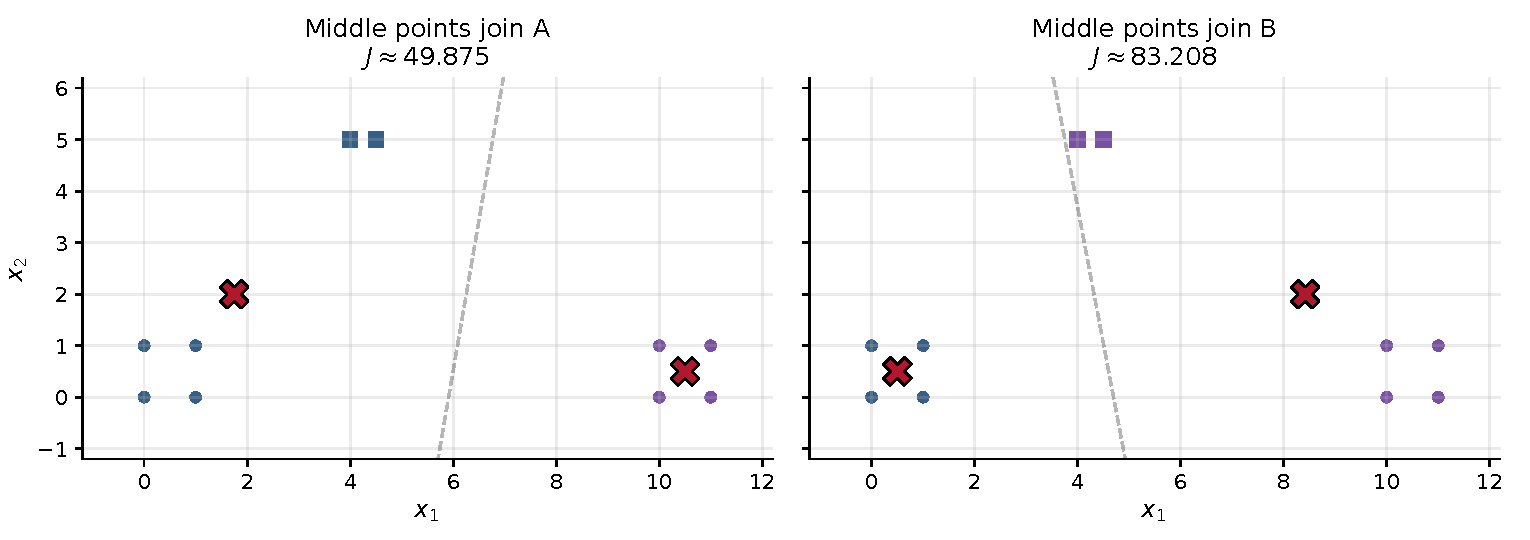
\includegraphics[width=\textwidth]{figures/handouts/em_algorithm/fig_kmeans_fixed_points}
  \caption{A toy $k$-means instance with two stable solutions depending on how the ambiguous ``middle'' points are assigned. Even in this simple setting, the update map has multiple basins and different fixed points can have different objective values.}
  \label{fig:kmeans-fixed-points}
\end{figure}

\Cref{fig:kmeans-fixed-points} makes the basin story visible.
The central points sit near an assignment boundary.
One initialization causes them to be claimed by the left cluster; another causes them to be claimed by the right cluster.
Once those assignments differ, the cluster means move differently, which reinforces the difference on the next E-step.
The stable solutions are therefore \emph{self-consistent latent assignments}.

This is exactly why initialization is part of the method rather than an afterthought.
In latent-variable problems one rarely hopes for a global theorem of the form ``EM converges to the best optimum from everywhere.''
Instead, the practical template is
\begin{algorithm}[H]
  \caption{Two-stage template: initialization + EM refinement}
  \label{alg:two-stage-em}
  \begin{algorithmic}[1]
    \Require Model class and EM operator $M_n$, plus a cheap initializer.
    \Ensure An estimate $\hat\theta$ intended to approximate a good population maximizer.
    \State \textbf{Initialization:} produce one or more candidates $\Theta_0$ (e.g.\ moments/spectral, $k$-means++, random restarts).
    \State Pick $\theta^{(0)}\in\Theta_0$ using a simple score (e.g.\ likelihood, held-out likelihood, or a surrogate).
    \State \textbf{Refinement:} run EM iterations $\theta^{(t+1)}=M_n(\theta^{(t)})$ until convergence; return the final iterate $\hat\theta$.
  \end{algorithmic}
\end{algorithm}

The Gaussian-mixture example later keeps the same logic but replaces hard assignments by soft responsibilities.
That makes the map smooth enough to analyze with derivatives, while preserving the same basin-versus-rate distinction.

\section[Gaussian mixture]{Example II: a two-component Gaussian mixture}
\label{sec:gmm-pop-em}

We now illustrate the contractive-map picture in the simplest EM setting: a balanced two-component Gaussian mixture with known variance.
To keep notation light, we work in one dimension and parameterize the unknown mean as $\theta^\star>0$; the model is
\[
Y \sim \tfrac12\,\mathcal{N}(\theta^\star,\sigma^2) + \tfrac12\,\mathcal{N}(-\theta^\star,\sigma^2),
\]
and we estimate $\theta\in\R$.
The latent variable is the component label.
This model makes the basin picture and the local-rate picture visible in the same calculation.
The same explicit map will explain why sign determines the basin and why separation controls the slope.

\subsection{EM operator and fixed points}
\label{subsec:gmm-em-operator}

Given a sample $\{y_i\}_{i=1}^n$, EM alternates between responsibilities
$w_\theta(y_i)=\Pr(Z=+1\mid Y=y_i,\theta)$ and maximizing the resulting quadratic surrogate $Q_n(\theta'\mid\theta)$.
In this model both steps have closed forms, so the update map is one-dimensional and explicit.

\subsubsection{Deriving the EM update in closed form}
\label{subsubsec:gmm-derivation}

We parameterize the mixture using a latent label $Z\in\{-1,+1\}$ with $\Pr(Z=+1)=\Pr(Z=-1)=1/2$ and
\[
Y\mid Z=z,\theta' \sim \mathcal{N}(z\theta',\sigma^2).
\]
The complete-data log-likelihood is (up to constants)
\[
\log f_{\theta'}(y,z) = -\frac{1}{2\sigma^2}\big(y-z\theta'\big)^2.
\]
By Bayes' rule, the responsibility is
\begin{align*}
w_\theta(y)
&=\Pr(Z=+1\mid Y=y,\theta)
=\frac{\exp\!\left(-\frac{(y-\theta)^2}{2\sigma^2}\right)}{\exp\!\left(-\frac{(y-\theta)^2}{2\sigma^2}\right)+\exp\!\left(-\frac{(y+\theta)^2}{2\sigma^2}\right)} \\
&=\frac{1}{1+\exp\!\left(-\frac{(y+\theta)^2-(y-\theta)^2}{2\sigma^2}\right)}
=\frac{1}{1+\exp\!\left(-\frac{2\theta y}{\sigma^2}\right)}.
\end{align*}
Here $(y+\theta)^2-(y-\theta)^2=4\theta y$, so the responsibility is a logistic function of $\theta y/\sigma^2$.
Equivalently,
\[
2w_\theta(y)-1 = \tanh\!\left(\frac{\theta y}{\sigma^2}\right),
\]
so the ``soft label'' $2w_\theta(y)-1$ is a smooth odd function of the score $\theta y$.

The sample $Q$-function is the conditional expectation of the complete-data log-likelihood,
\[
Q_n(\theta'\mid\theta)
=
-\frac{1}{2n\sigma^2}\sum_{i=1}^n\Big(
w_\theta(y_i)\,(y_i-\theta')^2 + (1-w_\theta(y_i))\,(y_i+\theta')^2
\Big),
\]
which is a concave quadratic function of $\theta'$.
Differentiate and set the derivative equal to $0$:
\[
0
=
\frac{\partial}{\partial \theta'}Q_n(\theta'\mid\theta)
=
\frac{1}{n\sigma^2}\sum_{i=1}^n\Big(
w_\theta(y_i)\,(y_i-\theta') - (1-w_\theta(y_i))\,(y_i+\theta')
\Big).
\]
Rearrange the term inside the sum as
\[
w_\theta(y_i)\,(y_i-\theta') - (1-w_\theta(y_i))\,(y_i+\theta')
=
\big(2w_\theta(y_i)-1\big)\,y_i-\theta',
\]
so the first-order condition becomes $0=\frac{1}{n\sigma^2}\sum_{i=1}^n\big(\big(2w_\theta(y_i)-1\big)\,y_i-\theta'\big)$.
Solving for $\theta'$ yields the closed-form M-step
\[
M_n(\theta)
=
\frac{1}{n}\sum_{i=1}^n \big(2w_\theta(y_i)-1\big)\,y_i
=
\frac{1}{n}\sum_{i=1}^n y_i\,\tanh\!\left(\frac{\theta y_i}{\sigma^2}\right).
\]
At the population level, the sample average is replaced by an expectation:
\[
M(\theta)
=
\E\!\left[\big(2w_\theta(Y)-1\big)\,Y\right]
=
\E\!\left[Y\,\tanh\!\left(\frac{\theta Y}{\sigma^2}\right)\right],
\]
yielding a deterministic update map $\theta^{t+1}=M(\theta^t)$.
This formula makes the geometry visible.
The score $\theta Y$ determines the posterior sign of the latent label, and the hyperbolic tangent turns that score into a soft label in $[-1,1]$.
When the mixture components are well separated, most draws of $Y$ make $\theta Y/\sigma^2$ large in magnitude, so the soft labels are close to $\pm 1$ and EM behaves almost like a hard assignment step.
When the components are weakly separated, the same soft labels stay closer to $0$, so the map lies nearer the diagonal and refinement is slower.

\begin{lemma}[Population fixed points for the symmetric mixture]
\label{lem:gmm-fixed-points}
Under the population model $Y=Z\theta^\star+\varepsilon$ with $Z\in\{-1,+1\}$ uniform and $\varepsilon\sim \mathcal{N}(0,\sigma^2)$ independent of $Z$, the population EM map satisfies
\[
M(\theta^\star)=\theta^\star,
\qquad
M(-\theta^\star)=-\theta^\star,
\qquad
M(0)=0.
\]
\end{lemma}

\begin{proof}
For any $\theta$, the posterior mean of the label is
\[
\E[Z\mid Y=y,\theta]
= (+1)\Pr(Z=+1\mid y,\theta) + (-1)\Pr(Z=-1\mid y,\theta)
=2w_\theta(y)-1.
\]
Therefore $M(\theta)=\E\!\left[Y\,\E[Z\mid Y,\theta]\right]$.
At $\theta=\theta^\star$, the conditional expectation is taken under the true model, so by the tower property
\[
M(\theta^\star)
=\E\!\left[Y\,\E[Z\mid Y,\theta^\star]\right]
=\E[YZ].
\]
Since $Y=Z\theta^\star+\varepsilon$ with $\varepsilon\perp Z$ and $Z^2=1$, we have $\E[YZ]=\E[(Z\theta^\star+\varepsilon)Z]=\theta^\star$.
The identity $M(-\theta^\star)=-\theta^\star$ follows by the same argument (or by symmetry of the model), and $M(0)=0$ follows because $w_0(y)=1/2$ so $2w_0(y)-1=0$.
\end{proof}

In this example the geometry assumption in \Cref{thm:em-fos-implies-contraction} is immediate:
the population objective $q(\theta')=Q(\theta'\mid\theta^\star)$ is a concave quadratic in $\theta'$ with second derivative $q''(\theta')=-1/\sigma^2$, hence it is globally $(1/\sigma^2)$-strongly concave.
The remaining step is to verify that the update map is stable in the basin of interest, which in one dimension reduces to controlling the slope $|M'(\theta)|$.

The third fixed point at $0$ plays a different role.
It is a self-consistent point in the sense that perfectly ambiguous responsibilities stay ambiguous, but it is not attractive.
The next exercise computes that instability directly.

\begin{exercise}[Instability of the zero fixed point in the Gaussian mixture map]
\label{ex:gmm-zero-unstable}
Consider the population EM map
\[
M(\theta)=\E\!\left[Y\,\tanh\!\left(\frac{\theta Y}{\sigma^2}\right)\right],
\qquad
Y=Z\theta^\star+\varepsilon,\ Z\in\{-1,+1\}\text{ uniform},\ \varepsilon\sim\mathcal{N}(0,\sigma^2).
\]
\begin{enumerate}[leftmargin=*]
  \item Show that $M$ is an odd function: $M(-\theta)=-M(\theta)$.
  \item Differentiate under the expectation to show
  \[
  M'(\theta)=\E\!\left[\frac{Y^2}{\sigma^2}\cdot \frac{1}{\cosh^2\!\left(\frac{\theta Y}{\sigma^2}\right)}\right].
  \]
  \item Compute $M'(0)$ and conclude that $0$ is a locally unstable fixed point (i.e.\ $|M'(0)|>1$).
\end{enumerate}
\end{exercise}

\SolutionBox[14]{%
\emph{Part (1).}
Using that $\tanh$ is odd,
\[
M(-\theta)
=\E\!\left[Y\,\tanh\!\left(-\frac{\theta Y}{\sigma^2}\right)\right]
=-\E\!\left[Y\,\tanh\!\left(\frac{\theta Y}{\sigma^2}\right)\right]
=-M(\theta).
\]

\emph{Part (2).}
Since $\frac{d}{du}\tanh(u)=\cosh^{-2}(u)$ and $\tanh,\cosh^{-2}$ are bounded, dominated convergence justifies differentiation under the expectation:
\[
M'(\theta)
=\E\!\left[Y\cdot \frac{Y}{\sigma^2}\cdot \frac{1}{\cosh^2\!\left(\frac{\theta Y}{\sigma^2}\right)}\right]
=\E\!\left[\frac{Y^2}{\sigma^2}\cdot \frac{1}{\cosh^2\!\left(\frac{\theta Y}{\sigma^2}\right)}\right].
\]

\emph{Part (3).}
At $\theta=0$, $\cosh^2(0)=1$, so $M'(0)=\E[Y^2]/\sigma^2$.
Under $Y=Z\theta^\star+\varepsilon$ with $Z^2=1$ and $\varepsilon\perp Z$,
\[
\E[Y^2]=\E[(Z\theta^\star+\varepsilon)^2]=(\theta^\star)^2+\sigma^2,
\]
so
\[
M'(0)=\frac{(\theta^\star)^2+\sigma^2}{\sigma^2}=1+\left(\frac{\theta^\star}{\sigma}\right)^2>1.
\]
Hence $0$ is a locally unstable fixed point.%
}

\Cref{fig:em-operator-fixed-points} now has a precise interpretation:
the graph shown there is exactly the map derived above.
The fixed points are its intersections with the diagonal.
Because the model is symmetric, the population log-likelihood has two equivalent maximizers $\pm\theta^\star$, and the sign of the initialization determines which one the iterates approach.
Here that nonconvexity is benign: the two limits differ only by label swapping, so they represent the same fitted mixture distribution.
Larger separation does not change the basin picture; it changes the rate of refinement within each basin.

\subsubsection{Global convergence of population EM in one dimension}
\label{subsubsec:gmm-global-population}

\Cref{fig:em-operator-fixed-points} suggests something stronger than local contraction near $\pm\theta^\star$: in one dimension, every initialization with the correct sign appears to converge to the corresponding population maximizer.
This is true, and it is a rare example where population EM admits a clean global guarantee.

To connect this claim with the literature, write the update map as a two-argument function.
For any $m>0$, let
\[
Y_m \sim \tfrac12\,\mathcal{N}(m,\sigma^2) + \tfrac12\,\mathcal{N}(-m,\sigma^2),
\qquad
M(\theta; m)\coloneqq \E\!\left[Y_m\,\tanh\!\left(\frac{\theta Y_m}{\sigma^2}\right)\right].
\]
Our population EM map is $\theta\mapsto M(\theta;\theta^\star)$, and (by the fixed point lemma) $M(m;m)=m$.

\begin{proposition}[Sign determines the basin in the 1D symmetric mixture]
\label{prop:gmm-global-population-sign-basin}
Assume $\theta^\star>0$.
Let $\theta^{(t+1)}=M(\theta^{(t)};\theta^\star)$ be the population EM iterates.
If $\theta^{(0)}>0$, then $\theta^{(t)}>0$ for all $t$ and $\theta^{(t)}\to \theta^\star$.
By symmetry, if $\theta^{(0)}<0$ then $\theta^{(t)}\to -\theta^\star$, and if $\theta^{(0)}=0$ then $\theta^{(t)}=0$ for all $t$.
\end{proposition}

\begin{proof}
If $\theta>0$, then $y\tanh(\theta y/\sigma^2)\ge 0$ for every $y$, with strict inequality for every $y\neq 0$.
Hence $M(\theta;\theta^\star)>0$, so positive initializations remain positive under the iteration.
The convergence claims are then exactly the one-dimensional specialization of \citet[Thms.~1--2]{xu_hsu_maleki_2016_global_em}: in one dimension, the sign condition $\ip{\theta^{(0)}}{\theta^\star}\gtrless 0$ reduces to $\theta^{(0)}\gtrless 0$, so the cited theorem says the population iterates converge to the corresponding signed maximizer, while the zero initialization remains at the unstable fixed point $0$.
\end{proof}

The same reference proves the higher-dimensional analogue, where the basin is determined by the sign of the inner product $\ip{\theta^{(0)}}{\theta^\star}$ rather than by the sign of a scalar initialization; see \citet[Thms.~1--2]{xu_hsu_maleki_2016_global_em}.

In one dimension, local contractivity near a fixed point is captured by the slope $|M'(\theta^\star)|$: smaller slope means faster refinement.
Since $M(\theta)=\E\!\left[Y\tanh\!\left(\frac{\theta Y}{\sigma^2}\right)\right]$ and $\frac{d}{du}\tanh(u)=\frac{1}{\cosh^2(u)}$, we can differentiate under the expectation to get
\[
M'(\theta)
=
\E\!\left[\frac{Y^2}{\sigma^2}\cdot \frac{1}{\cosh^2\!\left(\frac{\theta Y}{\sigma^2}\right)}\right].
\]
\Cref{fig:em-contraction-vs-snr} plots this slope as a function of the signal-to-noise ratio $\theta^\star/\sigma$ for the Gaussian mixture.
Separation plays the role of a \emph{conditioning parameter} for EM: when $\theta^\star/\sigma$ is large, responsibilities are close to $0$--$1$ under the true model and the map is strongly contractive, so refinement is fast; when $\theta^\star/\sigma$ is small, responsibilities stay near $1/2$ and the slope approaches $1$, so linear convergence becomes extremely slow.
Importantly, this ``slow EM'' regime is not a mysterious algorithmic failure---it reflects the fact that the statistical model itself becomes less distinctive as $\theta^\star/\sigma\to 0$:
the mixture distribution approaches a single Gaussian, so many parameter values yield almost the same observed-data likelihood and there is little signal for any method to exploit.
In other words, low separation is often ``easy'' in a \emph{model-fit} sense (many parameter values fit about equally well), but ``hard'' in a \emph{parameter-estimation} sense (it is difficult to reliably recover the tiny component separation).

\begin{lemma}[A simple sufficient condition for local contractivity]
\label{lem:gmm-contractive-region}
For any $\theta\neq 0$, the derivative satisfies
\[
0< M'(\theta) \le \frac{4e^{-2}\sigma^2}{\theta^2}.
\]
In particular, if $\theta^\star \ge \frac{4\sigma}{e}$, then $M$ is a contraction on the interval $\big[\frac{\theta^\star}{2},\frac{3\theta^\star}{2}\big]$ with contraction factor
\[
\kappa \le \frac{16e^{-2}\sigma^2}{(\theta^\star)^2} < 1.
\]
\end{lemma}

\clearpage
\begin{exercise}[Proving \Cref{lem:gmm-contractive-region}]
\label{ex:gmm-contractive-region}
Prove \Cref{lem:gmm-contractive-region}.
\emph{Hint:} start from $M'(\theta)=\E\!\left[\frac{Y^2}{\sigma^2}\cosh^{-2}\!\left(\frac{\theta Y}{\sigma^2}\right)\right]$,
use $\cosh(u)\ge \tfrac12 e^{|u|}$, and then maximize $y^2e^{-by}$ over $y\ge 0$ for $b>0$.
\end{exercise}

\SolutionBox[22]{%
Starting from
\[
M'(\theta)
=
\E\!\left[\frac{Y^2}{\sigma^2}\cdot \frac{1}{\cosh^2\!\left(\frac{\theta Y}{\sigma^2}\right)}\right],
\]
use $\cosh(u)\ge \tfrac12 e^{|u|}$ to obtain $\cosh^{-2}(u)\le 4e^{-2|u|}$.
Hence,
\[
M'(\theta)
\le
\frac{4}{\sigma^2}\E\!\left[Y^2\exp\!\left(-\frac{2|\theta|\,|Y|}{\sigma^2}\right)\right].
\]
Fix $b>0$.  For $y\ge 0$, the function $y\mapsto y^2e^{-by}$ has derivative $e^{-by}(2y-by^2)$, so it is maximized at $y=2/b$ with value $4e^{-2}/b^2$.
Therefore $Y^2e^{-b|Y|}\le 4e^{-2}/b^2$ almost surely, and with $b=\frac{2|\theta|}{\sigma^2}$ we get
\[
M'(\theta)
\le
\frac{4}{\sigma^2}\cdot \frac{4e^{-2}}{b^2}
=
\frac{4e^{-2}\sigma^2}{\theta^2}.
\]
If $\theta^\star\ge \frac{4\sigma}{e}$ and $\theta\in[\theta^\star/2,3\theta^\star/2]$, then $|\theta|\ge \theta^\star/2$ and the bound gives
\[
\sup_{\theta\in[\theta^\star/2,3\theta^\star/2]} M'(\theta)
\le
\frac{16e^{-2}\sigma^2}{(\theta^\star)^2}
<1,
\]
so $M$ is a contraction on this interval with contraction factor $\kappa\le 16e^{-2}\sigma^2/(\theta^\star)^2$.%
}

\begin{figure}[t]
  \centering
  \begin{tikzpicture}
  \begin{axis}[
    width=0.78\linewidth,
    height=5.8cm,
    xmin=0, xmax=3,
    ymin=0, ymax=1.02,
    axis lines=left,
    xlabel={$\theta^\star/\sigma$},
    ylabel={local slope $|M'(\theta^\star)|$},
    title={Gaussian mixture: contractivity strengthens with separation},
    title style={font=\small, yshift=-0.35em},
    clip=false,
  ]
    \addplot[stat221Blue,thick] table[row sep=\\] {
x y \\
0.000000 1 \\
0.020000 0.999200639318 \\
0.040000 0.996810196552 \\
0.060000 0.99285134851 \\
0.080000 0.987361104747 \\
0.100000 0.980389691245 \\
0.120000 0.971999101273 \\
0.140000 0.962261408213 \\
0.160000 0.951256940118 \\
0.180000 0.939072410763 \\
0.200000 0.925799089615 \\
0.220000 0.911531076495 \\
0.240000 0.896363728474 \\
0.260000 0.880392269087 \\
0.280000 0.863710594595 \\
0.300000 0.846410279611 \\
0.320000 0.828579775021 \\
0.340000 0.810303784702 \\
0.360000 0.791662803511 \\
0.380000 0.772732797077 \\
0.400000 0.753585003412 \\
0.420000 0.734285836967 \\
0.440000 0.714896877044 \\
0.460000 0.695474924141 \\
0.480000 0.676072109754 \\
0.500000 0.656736047028 \\
0.520000 0.637510011546 \\
0.540000 0.618433143276 \\
0.560000 0.599540662238 \\
0.580000 0.580864091861 \\
0.600000 0.562431485194 \\
0.620000 0.544267650154 \\
0.640000 0.526394370884 \\
0.660000 0.50883062299 \\
0.680000 0.491592781046 \\
0.700000 0.474694817242 \\
0.720000 0.45814849041 \\
0.740000 0.44196352504 \\
0.760000 0.426147780064 \\
0.780000 0.41070740746 \\
0.800000 0.395647000799 \\
0.820000 0.380969734022 \\
0.840000 0.36667749078 \\
0.860000 0.352770984743 \\
0.880000 0.339249871297 \\
0.900000 0.326112851098 \\
0.920000 0.313357765928 \\
0.940000 0.300981687329 \\
0.960000 0.288980998447 \\
0.980000 0.277351469548 \\
1.000000 0.266088327605 \\
1.020000 0.255186320385 \\
1.040000 0.244639775404 \\
1.060000 0.234442654114 \\
1.080000 0.224588601677 \\
1.100000 0.215070992637 \\
1.120000 0.205882972786 \\
1.140000 0.197017497522 \\
1.160000 0.188467366949 \\
1.180000 0.180225257954 \\
1.200000 0.17228375351 \\
1.220000 0.164635369393 \\
1.240000 0.157272578521 \\
1.260000 0.150187833083 \\
1.280000 0.143373584641 \\
1.300000 0.136822302343 \\
1.320000 0.130526489398 \\
1.340000 0.124478697942 \\
1.360000 0.118671542426 \\
1.380000 0.11309771162 \\
1.400000 0.107749979356 \\
1.420000 0.102621214102 \\
1.440000 0.097704387443 \\
1.460000 0.0929925815757 \\
1.480000 0.0884789958711 \\
1.500000 0.0841569525892 \\
1.520000 0.0800199018077 \\
1.540000 0.0760614256251 \\
1.560000 0.0722752416963 \\
1.580000 0.0686552061522 \\
1.600000 0.0651953159532 \\
1.620000 0.0618897107203 \\
1.640000 0.0587326740874 \\
1.660000 0.0557186346124 \\
1.680000 0.052842166284 \\
1.700000 0.0500979886587 \\
1.720000 0.0474809666585 \\
1.740000 0.044986110062 \\
1.760000 0.0426085727134 \\
1.780000 0.0403436514783 \\
1.800000 0.0381867849676 \\
1.820000 0.0361335520504 \\
1.840000 0.0341796701761 \\
1.860000 0.0323209935227 \\
1.880000 0.0305535109896 \\
1.900000 0.0288733440535 \\
1.920000 0.027276744506 \\
1.940000 0.0257600920913 \\
1.960000 0.0243198920608 \\
1.980000 0.0229527726556 \\
2.000000 0.0216554825256 \\
2.020000 0.0204248880892 \\
2.040000 0.019257970835 \\
2.060000 0.0181518245719 \\
2.080000 0.017103652636 \\
2.100000 0.0161107650723 \\
2.120000 0.0151705758106 \\
2.140000 0.0142805998594 \\
2.160000 0.0134384505301 \\
2.180000 0.0126418366964 \\
2.200000 0.0118885600784 \\
2.220000 0.0111765125314 \\
2.240000 0.0105036733215 \\
2.260000 0.00986810637488 \\
2.280000 0.00926795751283 \\
2.300000 0.00870145169878 \\
2.320000 0.00816689034165 \\
2.340000 0.00766264869717 \\
2.360000 0.00718717339248 \\
2.380000 0.00673898006967 \\
2.400000 0.00631665111137 \\
2.420000 0.00591883339061 \\
2.440000 0.0055442359866 \\
2.460000 0.00519162783269 \\
2.480000 0.00485983530513 \\
2.500000 0.00454773980721 \\
2.520000 0.00425427543351 \\
2.540000 0.00397842680007 \\
2.560000 0.00371922709277 \\
2.580000 0.00347575632804 \\
2.600000 0.00324713975739 \\
2.620000 0.00303254630428 \\
2.640000 0.00283118691814 \\
2.660000 0.00264231277163 \\
2.680000 0.00246521330105 \\
2.700000 0.00229921417106 \\
2.720000 0.00214367530193 \\
2.740000 0.001997989106 \\
2.760000 0.00186157903248 \\
2.780000 0.00173389843058 \\
2.800000 0.00161442964015 \\
2.820000 0.00150268314598 \\
2.840000 0.00139819661532 \\
2.860000 0.00130053368832 \\
2.880000 0.00120928249346 \\
2.900000 0.00112405397779 \\
2.920000 0.00104448023229 \\
2.940000 0.000970213019799 \\
2.960000 0.000900922663713 \\
2.980000 0.00083629734512 \\
3.000000 0.000776042723369 \\
    };

    \addplot[only marks,mark=*,mark size=1.3pt,stat221Orange] coordinates {
      (0.600000,0.562431485194)
      (2.000000,0.0216554825256)
    };
    \node[font=\small,anchor=south east] at (axis cs:0.600000,0.562431485194) {0.6};
    \node[font=\small,anchor=south west] at (axis cs:2.000000,0.0216554825256) {2};
  \end{axis}
\end{tikzpicture}

  \caption{Local contraction factor $|M'(\theta^\star)|$ for population EM in the symmetric two-component Gaussian mixture, as a function of the signal-to-noise ratio $\theta^\star/\sigma$. Larger separation leads to much stronger contractivity near the population maximizer, hence faster refinement once initialized in the correct basin.}
  \label{fig:em-contraction-vs-snr}
\end{figure}

\subsection{Local theory near a good fixed point}
\label{subsec:em-population-contractivity-template}

The Gaussian-mixture example already contains the shape of a general EM theorem.
Likelihood ascent is only part of the story.
It says that EM does not decrease the observed-data likelihood, but it does not say whether the initialization lies in the basin of a desirable fixed point, whether the population map pulls the iterates back once they are near that point, or whether finite-sample noise distorts that picture.
That is why useful EM results are usually local.

To study the local behavior near a good population fixed point $\theta^\star$, freeze the second argument of the surrogate at $\theta^\star$ and define
\[
q(\theta') \coloneqq Q(\theta' \mid \theta^\star).
\]
This is the surrogate EM would maximize if the E-step already used the correct posterior law.
From that viewpoint, the local theory is built out of two ideas.
First, the ideal objective $q$ should have enough curvature near $\theta^\star$ that maximizing it would correct small perturbations away from the target.
Second, the E-step should be stable: replacing $\theta^\star$ by a nearby iterate $\theta$ should not change the surrogate gradient too much.
If both statements hold, then the true EM map behaves like a perturbed maximization of $q$, so one can prove contraction for the population map and then transfer that result to the sample map by a perturbation argument.
The next definitions write those two ideas in a form suitable for the proof.

\begin{definition}[Local strong concavity]
\label{def:em-local-strong-concavity}
Fix $r>0$ and define the ball $B_r(\theta^\star)\coloneqq\{\theta\in\Theta:\norm{\theta-\theta^\star}_2\le r\}$.
We say $q$ is \textbf{$\lambda$-strongly concave on $B_r(\theta^\star)$} if for all $\theta_1,\theta_2\in B_r(\theta^\star)$,
\[
q(\theta_1)
\le
q(\theta_2)
\;+\;
\ip{\nabla q(\theta_2)}{\theta_1-\theta_2}
\;-\;
\frac{\lambda}{2}\norm{\theta_1-\theta_2}_2^2.
\]
\end{definition}

\begin{definition}[First-order stability (FOS)]
\label{def:em-fos}
Fix $r>0$.
We say the population $Q$-functions satisfy \textbf{$\mathrm{FOS}(\gamma)$ on $B_r(\theta^\star)$} if for all $\theta\in B_r(\theta^\star)$,
\[
\norm{\nabla_{\theta'} Q(M(\theta)\mid \theta^\star)-\nabla_{\theta'} Q(M(\theta)\mid \theta)}_2
\le
\gamma \norm{\theta-\theta^\star}_2.
\]
\end{definition}

\begin{theorem}[FOS + strong concavity $\Rightarrow$ contraction of population EM]
\label{thm:em-fos-implies-contraction}
Fix $r>0$ and define $B_r(\theta^\star)$ as in \Cref{def:em-local-strong-concavity}.
Assume:
\begin{enumerate}[leftmargin=*]
  \item $\theta^\star$ is self-consistent, meaning $M(\theta^\star)=\theta^\star$.
  \item $q(\cdot)=Q(\cdot\mid\theta^\star)$ is $\lambda$-strongly concave on $B_r(\theta^\star)$.
  \item $\mathrm{FOS}(\gamma)$ holds on $B_r(\theta^\star)$ for some $\gamma\in[0,\lambda)$.
  \item For all $\theta\in B_r(\theta^\star)$, the update $M(\theta)$ also lies in $B_r(\theta^\star)$.
  \item $\theta^\star$ is an interior maximizer of $q$, and for each $\theta\in B_r(\theta^\star)$ the EM update $M(\theta)$ is an interior maximizer of $\theta'\mapsto Q(\theta'\mid\theta)$, so that
  \[
  \nabla q(\theta^\star)=0,
  \qquad
  \nabla_{\theta'} Q(M(\theta)\mid\theta)=0.
  \]
\end{enumerate}
Then $M$ is contractive on $B_r(\theta^\star)$ with contraction factor $\kappa=\gamma/\lambda$:
\[
\norm{M(\theta)-\theta^\star}_2
\le
\frac{\gamma}{\lambda}\norm{\theta-\theta^\star}_2
\qquad\text{for all }\theta\in B_r(\theta^\star).
\]
\end{theorem}

\begin{proof}
Fix $\theta\in B_r(\theta^\star)$ and write $\bar\theta \coloneqq M(\theta)$.
By local invariance, $\bar\theta\in B_r(\theta^\star)$.
By \Cref{def:em-local-strong-concavity}, the function $-q$ is $\lambda$-strongly convex on $B_r(\theta^\star)$, so for all $u,v\in B_r(\theta^\star)$,
\[
\ip{\nabla q(u)-\nabla q(v)}{u-v}
\le
-\lambda\norm{u-v}_2^2,
\]
and therefore, by Cauchy--Schwarz,
\[
\lambda\norm{u-v}_2
\le
\norm{\nabla q(u)-\nabla q(v)}_2.
\]
Apply this with $u=\bar\theta$ and $v=\theta^\star$, and use $\nabla q(\theta^\star)=0$, to obtain
\[
\lambda\norm{\bar\theta-\theta^\star}_2
\le
\norm{\nabla q(\bar\theta)}_2
=
\norm{\nabla_{\theta'} Q(\bar\theta\mid\theta^\star)}_2.
\]
By the interior optimality condition $\nabla_{\theta'} Q(\bar\theta\mid\theta)=0$ and $\mathrm{FOS}(\gamma)$,
\[
\norm{\nabla_{\theta'} Q(\bar\theta\mid\theta^\star)}_2
=
\norm{\nabla_{\theta'} Q(\bar\theta\mid\theta^\star)-\nabla_{\theta'} Q(\bar\theta\mid\theta)}_2
\le
\gamma\norm{\theta-\theta^\star}_2.
\]
Combine the last two displays and divide by $\lambda$.
\end{proof}

In words, strong concavity tells us that the ideal M-step would correct deviations from $\theta^\star$, while FOS says the real E-step does not distort that ideal picture too much.
If FOS fails badly, then changing the current iterate can change the posterior weights so much that the update map loses its restorative pull.

\subsubsection{Gradient EM: an inexact M-step}
\label{subsec:em-gradient-em}

In large models, the exact maximization step defining $M(\theta)$ can be expensive.
A common alternative is to take one gradient ascent step on the surrogate $Q(\cdot\mid\theta)$ starting from $\theta$.
At the population level, this defines the \emph{gradient EM} operator
\[
G(\theta)\coloneqq \theta + \alpha\,\nabla_{\theta'} Q(\theta\mid\theta),
\]
where $\alpha>0$ is a step size.
(The sample version replaces $Q$ by $Q_n$.)

If we could take gradient ascent on the ideal objective $q(\theta)=Q(\theta\mid\theta^\star)$ directly, then strong concavity and smoothness would give a contraction for an appropriate step size; see \citep[\S9.2]{boyd_vandenberghe_2004_convex}.
Gradient EM behaves similarly when the surrogate gradient is stable near $\theta^\star$.

\begin{definition}[Gradient stability (GS)]
\label{def:em-gs}
Fix $r>0$.
We say the population $Q$-functions satisfy \textbf{$\mathrm{GS}(\gamma)$ on $B_r(\theta^\star)$} if for all $\theta\in B_r(\theta^\star)$,
\[
\norm{\nabla_{\theta'} Q(\theta\mid \theta^\star)-\nabla_{\theta'} Q(\theta\mid \theta)}_2
\le
\gamma \norm{\theta-\theta^\star}_2.
\]
\end{definition}

\begin{theorem}[GS + strong concavity $\Rightarrow$ contraction of gradient EM]
\label{thm:em-gs-implies-contraction}
Fix $r>0$ and assume:
\begin{enumerate}[leftmargin=*]
  \item $q(\cdot)=Q(\cdot\mid\theta^\star)$ is $\lambda$-strongly concave and $L$-smooth on $B_r(\theta^\star)$, with $0<\lambda\le L$.
  \item $\mathrm{GS}(\gamma)$ holds on $B_r(\theta^\star)$ for some $\gamma\in[0,\lambda)$.
  \item $\theta^\star$ is an interior maximizer of $q$, so $\nabla q(\theta^\star)=0$.
\end{enumerate}
Then gradient EM with step size $\alpha=\frac{2}{L+\lambda}$ is contractive on $B_r(\theta^\star)$:
\[
\norm{G(\theta)-\theta^\star}_2
\le
\left(\frac{L-\lambda+2\gamma}{L+\lambda}\right)\norm{\theta-\theta^\star}_2
\qquad\text{for all }\theta\in B_r(\theta^\star).
\]
\end{theorem}

\begin{proof}
Write $G(\theta)-\theta^\star$ as
\[
\underbrace{\theta + \alpha \nabla q(\theta)-\theta^\star}_{\text{gradient ascent on $q$}}
\;+\;
\alpha\underbrace{\bigl(\nabla_{\theta'} Q(\theta\mid\theta)-\nabla_{\theta'} Q(\theta\mid\theta^\star)\bigr)}_{\text{stability error}}.
\]
For $\alpha=\frac{2}{L+\lambda}$, gradient ascent on a $\lambda$-strongly concave, $L$-smooth function is a contraction mapping with factor $\frac{L-\lambda}{L+\lambda}$ (equivalently, apply the standard strongly convex result to $-q$).
Combine this with \Cref{def:em-gs} and $\alpha=\frac{2}{L+\lambda}$ to get
\[
\norm{G(\theta)-\theta^\star}_2
\le
\left(\frac{L-\lambda}{L+\lambda} + \frac{2\gamma}{L+\lambda}\right)\norm{\theta-\theta^\star}_2,
\]
which is the claim.
\end{proof}

Once a population contraction factor is available for either exact EM or gradient EM, the sample-level picture follows from a perturbation argument.

\begin{lemma}[Contraction + perturbation $\Rightarrow$ convergence to a neighborhood]
\label{lem:contraction-perturbation}
Fix a point $\theta^\star\in\Theta$ and a radius $r>0$.
Assume:
\begin{enumerate}[leftmargin=*]
  \item $M(\theta^\star)=\theta^\star$ and, for all $\theta$ with $\norm{\theta-\theta^\star}_2\le r$,
  \[
  \norm{M(\theta)-\theta^\star}_2 \le \kappa \norm{\theta-\theta^\star}_2
  \quad\text{for some }\kappa\in(0,1).
  \]
  \item For all $\theta$ with $\norm{\theta-\theta^\star}_2\le r$,
  \[
  \norm{M_n(\theta)-M(\theta)}_2 \le \varepsilon_n.
  \]
\end{enumerate}
Then any iterate sequence $\theta^{t+1}=M_n(\theta^t)$ that remains in the ball satisfies
\[
\norm{\theta^t-\theta^\star}_2
\le
\kappa^t \norm{\theta^0-\theta^\star}_2 + \frac{\varepsilon_n}{1-\kappa}.
\]
\end{lemma}

\begin{proof}
Write
\[
\norm{\theta^{t+1}-\theta^\star}_2
\le
\norm{M(\theta^t)-\theta^\star}_2 + \norm{M_n(\theta^t)-M(\theta^t)}_2
\le
\kappa\norm{\theta^t-\theta^\star}_2 + \varepsilon_n,
\]
then unroll the recursion.
\end{proof}

\Cref{lem:contraction-perturbation} is the core population-to-sample message.
Inside a basin where the sample map stays uniformly close to the population map, optimization error decays geometrically until it reaches a floor of order $\varepsilon_n/(1-\kappa)$.
Equivalently, sample EM converges to the sample fixed point in its basin, while the gap between that sample target and the population target is the residual statistical error.

\subsection{Finite-sample EM: geometric decay until a floor}
\label{sec:finite-sample-floor}

At finite $n$, the operator $M_n$ fluctuates around $M$.
In a neighborhood where $M$ is contractive and $M_n$ is uniformly close to $M$, \Cref{lem:contraction-perturbation} gives geometric decay until the remaining error is on the order of $1/\sqrt{n}$.

\begin{figure}[t]
  \centering
  \begin{tikzpicture}
  \begin{axis}[
    width=0.92\linewidth,
    height=6.2cm,
    xmin=0, xmax=22,
    ymode=log,
    axis lines=left,
    xlabel={EM iteration $t$},
    ylabel={distance $|\theta^{(t)}-\theta^\star|$},
    title={Gaussian mixture: geometric refinement until a sample-size floor},
    title style={font=\small, yshift=-0.35em},
    legend style={draw=stat221Gray!25, fill=white, fill opacity=0.95, text opacity=1},
    legend pos=north east,
    clip=false,
  ]
    \addplot[stat221Gray,thick,densely dashed] table[row sep=\\] {
x y \\
0.000000 1.8 \\
1.000000 1.09729288275 \\
2.000000 0.109028376417 \\
3.000000 0.00261865712788 \\
4.000000 5.68444330535e-05 \\
5.000000 1.23073156089e-06 \\
6.000000 2.63256854094e-08 \\
7.000000 2.43660647214e-10 \\
8.000000 3.21158211136e-10 \\
9.000000 3.33389760243e-10 \\
10.000000 3.33654437412e-10 \\
11.000000 3.33660210572e-10 \\
12.000000 3.33660654661e-10 \\
13.000000 3.33660654661e-10 \\
14.000000 3.33660654661e-10 \\
15.000000 3.33660654661e-10 \\
16.000000 3.33660654661e-10 \\
17.000000 3.33660654661e-10 \\
18.000000 3.33660654661e-10 \\
19.000000 3.33660654661e-10 \\
20.000000 3.33660654661e-10 \\
21.000000 3.33660654661e-10 \\
22.000000 3.33660654661e-10 \\
    };
    \addlegendentry{Population EM}

    % n=250
    \addplot[stat221Red,thick] table[row sep=\\] {
x y \\
0.000000 1.8 \\
1.000000 1.09872386901 \\
2.000000 0.110299246121 \\
3.000000 0.0505039018034 \\
4.000000 0.0515472428277 \\
5.000000 0.0515163642603 \\
6.000000 0.0515154249441 \\
7.000000 0.0515153981012 \\
8.000000 0.0515153973593 \\
9.000000 0.0515153973392 \\
10.000000 0.0515153973386 \\
11.000000 0.0515153973386 \\
12.000000 0.0515153973386 \\
13.000000 0.0515153973386 \\
14.000000 0.0515153973386 \\
15.000000 0.0515153973386 \\
16.000000 0.0515153973386 \\
17.000000 0.0515153973386 \\
18.000000 0.0515153973386 \\
19.000000 0.0515153973386 \\
20.000000 0.0515153973386 \\
21.000000 0.0515153973386 \\
22.000000 0.0515153973386 \\
    };
    \addlegendentry{$n=250$ (median)}
    \addplot[stat221Red!50,thin] table[row sep=\\] {
x y \\
0.000000 1.8 \\
1.000000 1.06088484132 \\
2.000000 0.0558003250334 \\
3.000000 0.0172269337719 \\
4.000000 0.0187376939554 \\
5.000000 0.0186938843451 \\
6.000000 0.0186928789526 \\
7.000000 0.0186928558916 \\
8.000000 0.0186928553628 \\
9.000000 0.0186928553507 \\
10.000000 0.0186928553504 \\
11.000000 0.0186928553504 \\
12.000000 0.0186928553504 \\
13.000000 0.0186928553504 \\
14.000000 0.0186928553504 \\
15.000000 0.0186928553504 \\
16.000000 0.0186928553504 \\
17.000000 0.0186928553504 \\
18.000000 0.0186928553504 \\
19.000000 0.0186928553504 \\
20.000000 0.0186928553504 \\
21.000000 0.0186928553504 \\
22.000000 0.0186928553504 \\
    };
    \addplot[stat221Red!50,thin] table[row sep=\\] {
x y \\
0.000000 1.8 \\
1.000000 1.13749626527 \\
2.000000 0.195839244443 \\
3.000000 0.110853135634 \\
4.000000 0.10599630166 \\
5.000000 0.105840011233 \\
6.000000 0.105834999751 \\
7.000000 0.105834838944 \\
8.000000 0.10583483378 \\
9.000000 0.105834833614 \\
10.000000 0.105834833609 \\
11.000000 0.105834833608 \\
12.000000 0.105834833608 \\
13.000000 0.105834833608 \\
14.000000 0.105834833608 \\
15.000000 0.105834833608 \\
16.000000 0.105834833608 \\
17.000000 0.105834833608 \\
18.000000 0.105834833608 \\
19.000000 0.105834833608 \\
20.000000 0.105834833608 \\
21.000000 0.105834833608 \\
22.000000 0.105834833608 \\
    };

    % n=1000
    \addplot[stat221Purple,thick] table[row sep=\\] {
x y \\
0.000000 1.8 \\
1.000000 1.0983030735 \\
2.000000 0.116403226832 \\
3.000000 0.0249846970799 \\
4.000000 0.0271994451237 \\
5.000000 0.0272440273864 \\
6.000000 0.027244923102 \\
7.000000 0.0272449411 \\
8.000000 0.0272449414617 \\
9.000000 0.027244941469 \\
10.000000 0.0272449414691 \\
11.000000 0.0272449414691 \\
12.000000 0.0272449414691 \\
13.000000 0.0272449414691 \\
14.000000 0.0272449414691 \\
15.000000 0.0272449414691 \\
16.000000 0.0272449414691 \\
17.000000 0.0272449414691 \\
18.000000 0.0272449414691 \\
19.000000 0.0272449414691 \\
20.000000 0.0272449414691 \\
21.000000 0.0272449414691 \\
22.000000 0.0272449414691 \\
    };
    \addlegendentry{$n=1000$ (median)}
    \addplot[stat221Purple!55,thin] table[row sep=\\] {
x y \\
0.000000 1.8 \\
1.000000 1.08333007975 \\
2.000000 0.0836193134053 \\
3.000000 0.0103829014241 \\
4.000000 0.00847228156732 \\
5.000000 0.00841108953049 \\
6.000000 0.00840974432263 \\
7.000000 0.00840971474938 \\
8.000000 0.00840971409918 \\
9.000000 0.00840971408488 \\
10.000000 0.00840971408457 \\
11.000000 0.00840971408456 \\
12.000000 0.00840971408456 \\
13.000000 0.00840971408456 \\
14.000000 0.00840971408456 \\
15.000000 0.00840971408456 \\
16.000000 0.00840971408456 \\
17.000000 0.00840971408456 \\
18.000000 0.00840971408456 \\
19.000000 0.00840971408456 \\
20.000000 0.00840971408456 \\
21.000000 0.00840971408456 \\
22.000000 0.00840971408456 \\
    };
    \addplot[stat221Purple!55,thin] table[row sep=\\] {
x y \\
0.000000 1.8 \\
1.000000 1.12615938693 \\
2.000000 0.165376411295 \\
3.000000 0.0472545773638 \\
4.000000 0.0455814764069 \\
5.000000 0.0455189731835 \\
6.000000 0.0455173198223 \\
7.000000 0.0455172765315 \\
8.000000 0.0455172754058 \\
9.000000 0.0455172753767 \\
10.000000 0.0455172753759 \\
11.000000 0.0455172753759 \\
12.000000 0.0455172753759 \\
13.000000 0.0455172753759 \\
14.000000 0.0455172753759 \\
15.000000 0.0455172753759 \\
16.000000 0.0455172753759 \\
17.000000 0.0455172753759 \\
18.000000 0.0455172753759 \\
19.000000 0.0455172753759 \\
20.000000 0.0455172753759 \\
21.000000 0.0455172753759 \\
22.000000 0.0455172753759 \\
    };

    % n=4000
    \addplot[stat221Blue,thick] table[row sep=\\] {
x y \\
0.000000 1.8 \\
1.000000 1.09776860352 \\
2.000000 0.106236150851 \\
3.000000 0.0150328312308 \\
4.000000 0.0136287629058 \\
5.000000 0.0136241329475 \\
6.000000 0.0136239966889 \\
7.000000 0.0136239929464 \\
8.000000 0.0136239928479 \\
9.000000 0.0136239928454 \\
10.000000 0.0136239928454 \\
11.000000 0.0136239928454 \\
12.000000 0.0136239928454 \\
13.000000 0.0136239928454 \\
14.000000 0.0136239928454 \\
15.000000 0.0136239928454 \\
16.000000 0.0136239928454 \\
17.000000 0.0136239928454 \\
18.000000 0.0136239928454 \\
19.000000 0.0136239928454 \\
20.000000 0.0136239928454 \\
21.000000 0.0136239928454 \\
22.000000 0.0136239928454 \\
    };
    \addlegendentry{$n=4000$ (median)}
    \addplot[stat221Blue!55,thin] table[row sep=\\] {
x y \\
0.000000 1.8 \\
1.000000 1.08188882734 \\
2.000000 0.0820973327345 \\
3.000000 0.00770508259319 \\
4.000000 0.0065464756106 \\
5.000000 0.00660028365008 \\
6.000000 0.00660143725538 \\
7.000000 0.00660146199262 \\
8.000000 0.00660146252319 \\
9.000000 0.00660146253458 \\
10.000000 0.00660146253482 \\
11.000000 0.00660146253483 \\
12.000000 0.00660146253483 \\
13.000000 0.00660146253483 \\
14.000000 0.00660146253483 \\
15.000000 0.00660146253483 \\
16.000000 0.00660146253483 \\
17.000000 0.00660146253483 \\
18.000000 0.00660146253483 \\
19.000000 0.00660146253483 \\
20.000000 0.00660146253483 \\
21.000000 0.00660146253483 \\
22.000000 0.00660146253483 \\
    };
    \addplot[stat221Blue!55,thin] table[row sep=\\] {
x y \\
0.000000 1.8 \\
1.000000 1.10460440298 \\
2.000000 0.12368330304 \\
3.000000 0.022890556425 \\
4.000000 0.022627348017 \\
5.000000 0.0226500740391 \\
6.000000 0.0226504929312 \\
7.000000 0.0226505004549 \\
8.000000 0.022650500585 \\
9.000000 0.0226505005871 \\
10.000000 0.0226505005871 \\
11.000000 0.0226505005871 \\
12.000000 0.0226505005871 \\
13.000000 0.0226505005871 \\
14.000000 0.0226505005871 \\
15.000000 0.0226505005871 \\
16.000000 0.0226505005871 \\
17.000000 0.0226505005871 \\
18.000000 0.0226505005871 \\
19.000000 0.0226505005871 \\
20.000000 0.0226505005871 \\
21.000000 0.0226505005871 \\
22.000000 0.0226505005871 \\
    };
  \end{axis}
\end{tikzpicture}

  \caption{Distance to $\theta^\star$ versus EM iteration in the Gaussian mixture example. Population EM converges linearly to $\theta^\star$. Sample EM tracks the population dynamics until it reaches a sample-dependent floor.}
  \label{fig:em-pop-vs-sample}
\end{figure}

In this example, once the initialization lands in the correct basin, the population map is contractive and the sample map tracks it until the iterate reaches an $n$-dependent statistical floor.
Separation does not change which basin is correct; it changes the speed of refinement inside that basin.

A systematic development of this population-to-sample contraction argument appears in \citet[Thm.~1]{balakrishnan_wainwright_yu_2014_em}.
Moreover, this two-Gaussian mixture is one of the rare latent-variable models where much stronger \emph{global} guarantees are possible; see, e.g., \citet[Thm.~1]{xu_hsu_maleki_2016_global_em}.

\clearpage
% ------------------------------------------------------------
\section[Missing covariates]{Example III: regression with missing covariates}
\label{sec:missing-covariates}

EM is also natural outside mixture models whenever part of the data is latent or unobserved.
A basic example is linear regression with covariates missing completely at random.
Let $X\in\R^d$ and $Y\in\R$ follow the population model
\[
X \sim \mathcal{N}(0,I_d),
\qquad
Y = \ip{X}{\theta^\star} + \varepsilon,
\qquad
\varepsilon \sim \mathcal{N}(0,\sigma^2)\ \text{independent of }X,
\]
and suppose we observe $Y$ but only a subset of the coordinates of $X$.
Formally, each coordinate is missing with probability $\rho\in[0,1)$, independently across coordinates and samples.
The missing coordinates are treated as latent variables, so EM alternates between imputing them from the conditional law of $X$ given $(X_{\mathrm{obs}},Y)$ and refitting $\theta'$ by weighted least squares using the conditional moments $\E[X\mid X_{\mathrm{obs}},Y,\theta]$ and $\E[XX^\top\mid X_{\mathrm{obs}},Y,\theta]$.

This example complements the Gaussian mixture.
In the mixture model, weak separation mainly makes the EM map flatter near the correct target.
Here the more basic issue is that the E-step literally fills in unseen coordinates using the \emph{current} parameter.
If $\theta$ is already close to $\theta^\star$, those imputations are helpful.
If $\theta$ points in a badly wrong direction and the missingness level is high, the imputations can reinforce that wrong direction, so the map itself can develop a bad stable fixed point.

\subsection{Missingness and identifiability}
\label{subsec:missing-covariates-identifiability-limit}

As $\rho$ increases, fewer coordinates of $X$ are observed, the E-step becomes less informative, and both optimization and statistical estimation become harder.

The extreme case $\rho=1$ shows the identifiability issue most clearly.
If all covariates are missing, then the observed data are only the responses $\{Y_i\}_{i=1}^n$.
Because $X\sim\mathcal{N}(0,I_d)$, for any parameter $\theta$ we have $\ip{X}{\theta}\sim \mathcal{N}(0,\norm{\theta}_2^2)$, so
\[
Y \mid \theta
\sim
\mathcal{N}\!\big(0,\norm{\theta}_2^2+\sigma^2\big).
\]
Therefore the distribution of the observed data depends on $\theta$ only through $\norm{\theta}_2$.
In particular, the direction of $\theta^\star$ is \emph{not identifiable}: any $\tilde\theta$ with $\norm{\tilde\theta}_2=\norm{\theta^\star}_2$ produces the same law for $Y$.
No algorithm (EM included) can recover what the data do not contain; at best, one can hope to estimate $\norm{\theta^\star}_2$.
\Cref{fig:em-nonidentifiability-ridge} gives a schematic picture.

\begin{figure}[t]
  \centering
  \begin{tikzpicture}
  \begin{axis}[
    width=0.62\linewidth,
    height=6.0cm,
    axis lines=middle,
    xmin=-1.6, xmax=1.6,
    ymin=-1.6, ymax=1.6,
    xlabel={$\theta_1$},
    ylabel={$\theta_2$},
    xtick=\empty,
    ytick=\empty,
    clip=false,
  ]
    \addplot[stat221Blue,thick,domain=0:360,samples=200] ({cos(x)}, {sin(x)});

    \addplot[only marks,mark=*,mark size=1.2pt,stat221Red] coordinates {(1,0)};
    \node[
      font=\small,
      anchor=south west,
      fill=white,
      fill opacity=0.92,
      text opacity=1,
      inner sep=1pt,
      rounded corners=1pt,
    ] at (axis cs:1.050000,0.080000) {$\theta^\star$};

    \addplot[only marks,mark=*,mark size=1.2pt,stat221Purple] coordinates {(0,1)};
    \node[
      font=\small,
      anchor=south east,
      fill=white,
      fill opacity=0.92,
      text opacity=1,
      inner sep=1pt,
      rounded corners=1pt,
    ] at (axis cs:-0.040000,1.070000) {$\tilde\theta$};

    \node[
      font=\small,
      align=center,
      stat221Gray,
      fill=white,
      fill opacity=0.92,
      text opacity=1,
      inner sep=1.5pt,
      rounded corners=1pt,
    ] at (axis cs:0,-1.420000) {same observed law\\(same $\|\theta\|_2$)};
  \end{axis}
\end{tikzpicture}

  \caption{Non-identifiability in the ``noise-only'' limit.  When $\rho=1$, we never observe any coordinates of $X$, and the marginal law is $Y\mid\theta\sim\mathcal{N}(0,\norm{\theta}_2^2+\sigma^2)$.  Hence all parameters on a sphere $\{\theta:\norm{\theta}_2=\text{const}\}$ induce the same distribution of $Y$, so there cannot be a contraction toward a unique maximizer.}
  \label{fig:em-nonidentifiability-ridge}
\end{figure}

This illustrates a different failure mode than low separation in mixtures.
In Example II, low separation mainly means weak identification and poor conditioning: there is a well-defined population target up to the sign symmetry, but the likelihood is relatively flat and the EM contraction factor is close to $1$, so refinement is slow and statistical accuracy requires very large $n$.
Here, increasing missingness pushes the statistical problem itself toward non-identifiability, so EM no longer has a unique population target to contract toward.

\subsection{Deriving the EM operator in closed form}
\label{subsec:missing-covariates-derivation}

Because the model is Gaussian, the E-step conditional moments can be written explicitly and the M-step reduces to a linear system.
These formulas show exactly where the self-reinforcement enters:
the posterior moments used in the E-step depend on the current iterate $\theta$, so the regression problem solved by the M-step is built out of \emph{imputed} covariates that already reflect the current belief.

\subsubsection{E-step: conditional moments from a joint Gaussian}
\label{subsubsec:missing-covariates-estep}

Fix one observation $(x_{\mathrm{obs}},y)$ and let $O\subseteq\{1,\dots,d\}$ be the set of observed coordinates, with $M$ its complement.
Write the parameter and covariate vector in blocks $\theta=(\theta_M,\theta_O)$ and $X=(X_M,X_O)$.
Conditioned on $X_O=x_O$, the scalar response model under parameter $\theta$ is
\[
Y = \ip{\theta_O}{x_O} + \ip{\theta_M}{X_M} + \varepsilon,
\qquad
X_M\sim\mathcal{N}(0,I),
\qquad
\varepsilon\sim\mathcal{N}(0,\sigma^2),
\]
so $X_M\mid (X_O=x_O,Y=y,\theta)$ is the Gaussian posterior in a one-dimensional linear measurement model.
A standard conditioning calculation (e.g.\ via Sherman--Morrison) yields
\begin{align}
\label{eq:missing-covariates-posterior-mean}
\E[X_M\mid x_O,y,\theta]
&=
\frac{\theta_M}{\sigma^2+\norm{\theta_M}_2^2}\,\Big(y-\ip{\theta_O}{x_O}\Big), \\
\label{eq:missing-covariates-posterior-cov}
\mathrm{Cov}(X_M\mid x_O,y,\theta)
&=
I-\frac{\theta_M\theta_M^\top}{\sigma^2+\norm{\theta_M}_2^2}.
\end{align}

Define the conditional mean and second moment of the \emph{full} covariate vector,
\[
\mu_\theta(x_{\mathrm{obs}},y)\coloneqq \E[X\mid X_{\mathrm{obs}}=x_{\mathrm{obs}},Y=y,\theta],
\qquad
\Sigma_\theta(x_{\mathrm{obs}},y)\coloneqq \E[XX^\top\mid X_{\mathrm{obs}}=x_{\mathrm{obs}},Y=y,\theta].
\]
Then $\mu_\theta$ agrees with the observed coordinates and uses \eqref{eq:missing-covariates-posterior-mean} for the missing coordinates:
\[
(\mu_\theta)_O = x_O,
\qquad
(\mu_\theta)_M = \E[X_M\mid x_O,y,\theta].
\]
Similarly, $\Sigma_\theta$ is obtained by combining the posterior covariance \eqref{eq:missing-covariates-posterior-cov} with the rank-one term from the posterior mean:
\[
(\Sigma_\theta)_{MM}
=
\mathrm{Cov}(X_M\mid x_O,y,\theta) + \E[X_M\mid x_O,y,\theta]\E[X_M\mid x_O,y,\theta]^\top,
\qquad
(\Sigma_\theta)_{OO}=x_Ox_O^\top,
\]
and the cross moments satisfy $(\Sigma_\theta)_{MO}=\E[X_M\mid x_O,y,\theta]\,x_O^\top$ and $(\Sigma_\theta)_{OM}=x_O\,\E[X_M\mid x_O,y,\theta]^\top$.

\clearpage
This Gaussian-conditioning algebra is the exact E-step calculation underlying the formulas above.
\begin{exercise}[Deriving the E-step conditional moments in the missing-covariates model]
\label{ex:missing-covariates-estep}
In \Cref{subsubsec:missing-covariates-estep}, fix a set of observed coordinates $O$ with complement $M$, and fix one observation $(x_O,y)$.
Consider the linear-Gaussian model
\[
X_M\sim\mathcal{N}(0,I),
\qquad
Y=\ip{\theta_O}{x_O}+\ip{\theta_M}{X_M}+\varepsilon,
\qquad
\varepsilon\sim\mathcal{N}(0,\sigma^2)\ \text{independent of }X_M.
\]
Show that the posterior is Gaussian with mean and covariance
\[
\E[X_M\mid x_O,y,\theta]=\frac{\theta_M}{\sigma^2+\norm{\theta_M}_2^2}\,\Big(y-\ip{\theta_O}{x_O}\Big),
\qquad
\mathrm{Cov}(X_M\mid x_O,y,\theta)=I-\frac{\theta_M\theta_M^\top}{\sigma^2+\norm{\theta_M}_2^2}.
\]
\emph{Hint:} write $(X_M,\;Y-\ip{\theta_O}{x_O})$ as a jointly Gaussian pair and use the standard conditional Gaussian formula.
\end{exercise}

\SolutionBox[18]{%
This is the standard conditional-Gaussian calculation behind the E-step.
Define the centered scalar $\tilde Y\coloneqq Y-\ip{\theta_O}{x_O}=\ip{\theta_M}{X_M}+\varepsilon$.
Then $(X_M,\tilde Y)$ is jointly Gaussian with
\[
\E[X_M]=0,
\qquad
\E[\tilde Y]=0,
\qquad
\mathrm{Cov}(X_M)=I.
\]
Moreover,
\[
\mathrm{Cov}(X_M,\tilde Y)
=
\E[X_M(\theta_M^\top X_M+\varepsilon)]
=
\E[X_M X_M^\top]\theta_M
=\theta_M,
\]
and
\[
\mathrm{Var}(\tilde Y)
=
\mathrm{Var}(\theta_M^\top X_M)+\mathrm{Var}(\varepsilon)
=
\norm{\theta_M}_2^2+\sigma^2.
\]
For a jointly Gaussian pair $(U,V)$ with $\mathrm{Var}(V)>0$, the conditional law is
\[
U\mid(V=v)\sim \mathcal{N}\!\left(\mathrm{Cov}(U,V)\,\mathrm{Var}(V)^{-1}v,\;\mathrm{Cov}(U)-\mathrm{Cov}(U,V)\,\mathrm{Var}(V)^{-1}\mathrm{Cov}(V,U)\right).
\]
Apply this with $U=X_M$ and $V=\tilde Y$ to obtain
\[
\E[X_M\mid \tilde Y=\tilde y]=\frac{\theta_M}{\sigma^2+\norm{\theta_M}_2^2}\,\tilde y,
\qquad
\mathrm{Cov}(X_M\mid \tilde Y)=I-\frac{\theta_M\theta_M^\top}{\sigma^2+\norm{\theta_M}_2^2}.
\]
Substitute $\tilde y=y-\ip{\theta_O}{x_O}$ to match \eqref{eq:missing-covariates-posterior-mean}--\eqref{eq:missing-covariates-posterior-cov}.%
}
\subsubsection{M-step: a quadratic \texorpdfstring{$Q_n$}{Qn} and a linear system}
\label{subsubsec:missing-covariates-mstep}

The complete-data log-likelihood for a single pair $(x,y)$ is
\[
\log f_{\theta'}(x,y)
=
C
-\frac{1}{2}\norm{x}_2^2
-\frac{1}{2\sigma^2}\big(y-\ip{x}{\theta'}\big)^2.
\]
In the $Q$-function, we take the conditional expectation over the missing covariates under the current iterate $\theta$.
The term $\norm{x}_2^2$ does not depend on $\theta'$, and the factor $1/\sigma^2$ does not affect the argmax, so it is enough to expand the expected squared error.
For one observation,
\begin{align*}
\E\Big[\big(y-\ip{X}{\theta'}\big)^2\mid x_{\mathrm{obs}},y,\theta\Big]
&=
y^2 - 2y\,\ip{\E[X\mid x_{\mathrm{obs}},y,\theta]}{\theta'}
  + \E\big[\theta'^\top XX^\top \theta'\mid x_{\mathrm{obs}},y,\theta\big] \\
&=
y^2 - 2y\,\ip{\mu_\theta(x_{\mathrm{obs}},y)}{\theta'}
  + \theta'^\top \Sigma_\theta(x_{\mathrm{obs}},y)\,\theta'.
\end{align*}
Summing over samples, and dropping additive constants that do not affect the maximizer, yields the quadratic form
\[
Q_n(\theta'\mid\theta)
=
-\frac{1}{2n}\sum_{i=1}^n
\Big(\theta'^\top \Sigma_\theta(x_{\mathrm{obs},i},y_i)\,\theta'
-2y_i\,\ip{\mu_\theta(x_{\mathrm{obs},i},y_i)}{\theta'}\Big).
\]
Taking a gradient in $\theta'$ and setting it equal to zero gives a linear system for the M-step:
\[
\left(\frac{1}{n}\sum_{i=1}^n \Sigma_\theta(x_{\mathrm{obs},i},y_i)\right)\theta'
=
\frac{1}{n}\sum_{i=1}^n y_i\,\mu_\theta(x_{\mathrm{obs},i},y_i),
\]
so, whenever the averaged conditional second-moment matrix is invertible, the unique sample M-step is
\[
M_n(\theta)
=
\left(\frac{1}{n}\sum_{i=1}^n \Sigma_\theta(x_{\mathrm{obs},i},y_i)\right)^{-1}
\left(\frac{1}{n}\sum_{i=1}^n y_i\,\mu_\theta(x_{\mathrm{obs},i},y_i)\right).
\]
The population operator $M$ has the same form with empirical averages replaced by expectations, again when the corresponding population matrix is nonsingular.
Here the relationship between $M$ and $M_n$ is direct: $M_n$ is the perturbation produced by replacing expectations with sample averages.

As a useful check, if there is no missingness ($\rho=0$), then $\mu_\theta(x_{\mathrm{obs}},y)=x$ and $\Sigma_\theta(x_{\mathrm{obs}},y)=xx^\top$ regardless of $\theta$, so $M_n(\theta)$ reduces to ordinary least squares and does not depend on the current iterate.

\subsubsection{A one-dimensional verification: explicit population map and local slope}
\label{subsubsec:missing-covariates-1d-check}

The full verification of contractivity for the missing-covariates model is algebraically involved in general dimension.
In one dimension the population EM map has a closed form, so the stability calculation can be carried out directly.
As in the Gaussian mixture, the population objective $q(\theta')=Q(\theta'\mid\theta^\star)$ is a concave quadratic in $\theta'$ with Hessian $-\sigma^{-2}I$, so the main issue is not the local geometry of $q$ but the stability of the E-step as $\theta$ varies.

Assume $d=1$.
Each sample either reveals $X$ (with probability $1-\rho$) or hides it (with probability $\rho$), and we always observe $Y=\theta^\star X+\varepsilon$.
When $X$ is missing, the E-step uses the Gaussian posterior under the current iterate $\theta$:
\[
X\mid (Y=y,\theta) \sim \mathcal{N}\!\left(\frac{\theta}{\theta^2+\sigma^2}y,\;\frac{\sigma^2}{\theta^2+\sigma^2}\right),
\]
so
\[
\mu_\theta(y) \coloneqq \E[X\mid Y=y,\theta] = \frac{\theta}{\theta^2+\sigma^2}y,
\qquad
\Sigma_\theta(y) \coloneqq \E[X^2\mid Y=y,\theta]
=
\frac{\sigma^2}{\theta^2+\sigma^2}+\mu_\theta(y)^2.
\]
When $X$ is observed, we simply have $\mu_\theta(x,y)=x$ and $\Sigma_\theta(x,y)=x^2$.

At the population level, the M-step takes the same linear-system form as above, which in one dimension simplifies to
\[
M(\theta)
=
\frac{\E\!\left[Y\,\mu_\theta(X_{\mathrm{obs}},Y)\right]}{\E\!\left[\Sigma_\theta(X_{\mathrm{obs}},Y)\right]}.
\]
Using the missingness decomposition and the identities
$\E[YX]=\theta^\star$, $\E[X^2]=1$, and $\E[Y^2]=(\theta^\star)^2+\sigma^2$, we obtain
\begin{align}
\label{eq:missing-covariates-1d-pop-map}
M(\theta)
&=
\frac{(1-\rho)\,\theta^\star
\;+\;\rho\,\frac{\theta}{\theta^2+\sigma^2}\big((\theta^\star)^2+\sigma^2\big)}
{(1-\rho)\cdot 1
\;+\;\rho\left(\frac{\sigma^2}{\theta^2+\sigma^2}
\;+\;\frac{\theta^2}{(\theta^2+\sigma^2)^2}\big((\theta^\star)^2+\sigma^2\big)\right)}.
\end{align}
Plugging in $\theta=\theta^\star$ gives $M(\theta^\star)=\theta^\star$ (the numerator becomes $\theta^\star$ and the denominator becomes $1$).

The structure of \eqref{eq:missing-covariates-1d-pop-map} is revealing.
The fully observed fraction $(1-\rho)$ contributes a direct pull toward $\theta^\star$.
The missing fraction $\rho$ contributes a term proportional to
\[
\frac{\theta}{\theta^2+\sigma^2},
\]
which depends on the \emph{current iterate}.
That is the self-reinforcing part of EM in this model:
when a covariate is unobserved, the E-step replaces it by a conditional mean whose sign and magnitude are already filtered through $\theta$.
At small $\rho$ the observed-data pull dominates.
At large $\rho$, the feedback through the current iterate can become strong enough to create additional fixed points.

We can also differentiate \eqref{eq:missing-covariates-1d-pop-map} to quantify the local contraction factor.
Write $M(\theta)=N(\theta)/D(\theta)$, where
\[
N(\theta) \coloneqq (1-\rho)\,\theta^\star + \rho\,\frac{\theta}{\theta^2+\sigma^2}\big((\theta^\star)^2+\sigma^2\big),
\]
and
\[
D(\theta)\coloneqq (1-\rho)+\rho\left(\frac{\sigma^2}{\theta^2+\sigma^2}
+\frac{\theta^2}{(\theta^2+\sigma^2)^2}\big((\theta^\star)^2+\sigma^2\big)\right).
\]
Then $N(\theta^\star)=\theta^\star$ and $D(\theta^\star)=1$.
Differentiate:
\[
N'(\theta)
=
\rho\big((\theta^\star)^2+\sigma^2\big)\cdot \frac{\sigma^2-\theta^2}{(\theta^2+\sigma^2)^2},
\]
and
\[
D'(\theta)
=
\rho\left(
-\frac{2\sigma^2\theta}{(\theta^2+\sigma^2)^2}
+2\big((\theta^\star)^2+\sigma^2\big)\cdot \frac{\theta(\sigma^2-\theta^2)}{(\theta^2+\sigma^2)^3}
\right).
\]
Evaluating at $\theta=\theta^\star$ and using the quotient rule gives
\[
M'(\theta^\star)
=
\frac{N'(\theta^\star)D(\theta^\star)-N(\theta^\star)D'(\theta^\star)}{D(\theta^\star)^2}
=
N'(\theta^\star)-\theta^\star D'(\theta^\star)
=
\rho\,\frac{(\theta^\star)^4+\sigma^4}{\big((\theta^\star)^2+\sigma^2\big)^2}.
\]
In particular, since $(\theta^\star)^4+\sigma^4 \le \big((\theta^\star)^2+\sigma^2\big)^2$, we have $0<M'(\theta^\star)\le \rho$.
In this simplest case, the local contraction factor worsens roughly linearly with the missingness probability $\rho$.
It equals $0$ when $\rho=0$, reflecting the fact that in the fully observed model the population M-step jumps to $\theta^\star$ in one iteration.

\subsubsection{A sharp counterexample: a spurious stable fixed point at high missingness}
\label{subsubsec:missing-covariates-spurious-fixed-point}

The local-slope calculation above can make it seem as if missingness only slows EM down.
However, even in one dimension (where the model is identifiable for every $\rho<1$), the population EM map can have \emph{multiple} stable fixed points when $\rho$ is large.
This is a genuinely nonconvex phenomenon: it is present even at the population level, so it cannot be blamed on finite-sample noise.

To see this explicitly, fix $\theta^\star=1$ and $\sigma=1$.
For $\rho=0.95$, the closed-form population map \eqref{eq:missing-covariates-1d-pop-map} becomes a rational function $M(\theta)$.
Define $f(\theta)\coloneqq M(\theta)-\theta$.

\clearpage
\begin{exercise}[A spurious fixed point from high missingness (1D)]
\label{ex:missing-covariates-spurious-fixed-point}
In the one-dimensional setting with $\theta^\star=\sigma=1$ and $\rho=0.95$, consider the population map \eqref{eq:missing-covariates-1d-pop-map} and define $f(\theta)=M(\theta)-\theta$.
\begin{enumerate}[leftmargin=*]
  \item Compute $f(-1)$ and $f(-0.5)$, and use the intermediate value theorem to show that $M$ has a fixed point in $(-1,-0.5)$.
  \item Compute $f(-0.1)$ and $f(0)$, and show that $M$ has a fixed point in $(-0.1,0)$.
  \item Explain why this implies that the population map has at least three fixed points for this parameter choice.
\end{enumerate}
\end{exercise}

\SolutionBox[22]{%
We use the closed form \eqref{eq:missing-covariates-1d-pop-map} with $\theta^\star=\sigma=1$ and $\rho=0.95$.

\emph{Part (1).}
For $\theta=-1$, note that $\theta^2+\sigma^2=2$ and $(\theta^\star)^2+\sigma^2=2$, so the numerator is
\[
(1-\rho)\theta^\star+\rho\,\frac{\theta}{\theta^2+\sigma^2}\big((\theta^\star)^2+\sigma^2\big)
=0.05\cdot 1+0.95\cdot\frac{-1}{2}\cdot 2
=-0.9,
\]
and the denominator is $0.05+0.95\cdot(1/2+1/2)=1$.
Thus $M(-1)=-0.9$ and $f(-1)=M(-1)-(-1)=0.1>0$.

For $\theta=-0.5$, we have $\theta^2+\sigma^2=1.25$ and $(\theta^\star)^2+\sigma^2=2$.
The numerator is
\[
0.05\cdot 1+0.95\cdot\frac{-0.5}{1.25}\cdot 2
=0.05-0.76
=-0.71,
\]
and the denominator is
\[
0.05+0.95\left(\frac{1}{1.25}+\frac{0.25}{1.25^2}\cdot 2\right)
=0.05+0.95(0.8+0.32)
=0.05+1.064
=1.114.
\]
Therefore $M(-0.5)\approx -0.71/1.114\approx -0.637$ and $f(-0.5)\approx -0.137<0$.
Since $f$ is continuous, there exists $\bar\theta\in(-1,-0.5)$ with $f(\bar\theta)=0$, i.e.\ $M(\bar\theta)=\bar\theta$.

\emph{Part (2).}
At $\theta=0$, the numerator is $(1-\rho)\theta^\star=0.05$ and the denominator is $(1-\rho)+\rho=1$, so $M(0)=0.05$ and $f(0)>0$.
At $\theta=-0.1$, we have $\theta^2+\sigma^2=1.01$ and $(\theta^\star)^2+\sigma^2=2$.
The numerator is
\[
0.05\cdot 1+0.95\cdot\frac{-0.1}{1.01}\cdot 2
\approx 0.05-0.188
\approx -0.138,
\]
and the denominator is
\[
0.05+0.95\left(\frac{1}{1.01}+\frac{0.01}{1.01^2}\cdot 2\right)
\approx 0.05+0.95(0.990+0.020)
\approx 1.009.
\]
Thus $M(-0.1)\approx -0.138/1.009\approx -0.137$ and $f(-0.1)\approx -0.037<0$.
By continuity, there is a fixed point in $(-0.1,0)$.

\emph{Part (3).}
Together with the true fixed point $M(\theta^\star)=\theta^\star=1$, this shows the population map has at least three distinct fixed points for this parameter choice.%
}

\Cref{fig:em-missing-1d-spurious-fixed-points} plots $M(\theta)$ and the diagonal.
Numerically, the three fixed points are at
\[
\theta^\star=1,
\qquad
\bar\theta_{\mathrm{bad}}\approx -0.820,
\qquad
\bar\theta_{\mathrm{sep}}\approx -0.056.
\]
Their local stability is determined by the slope $|M'(\bar\theta)|$: a fixed point is locally stable if $|M'(\bar\theta)|<1$.
For this example, $|M'(1)|\approx 0.475$ and $|M'(\bar\theta_{\mathrm{bad}})|\approx 0.465$, so both are stable, while $|M'(\bar\theta_{\mathrm{sep}})|\approx 1.87$, so $\bar\theta_{\mathrm{sep}}$ is unstable and acts as a basin separator.
Thus, for some initializations (e.g.\ large negative $\theta^{(0)}$), population EM converges to the \emph{wrong} stable point $\bar\theta_{\mathrm{bad}}$ rather than to $\theta^\star$.

\begin{figure}[t]
  \centering
  \begin{tikzpicture}
  \begin{axis}[
    width=0.82\linewidth,
    height=6.4cm,
    xmin=-2.5, xmax=1.5,
    ymin=-2.5, ymax=1.5,
    axis lines=left,
    xlabel={$\theta$},
    ylabel={$M(\theta)$},
    title={Missing covariates (1D, $\rho=0.95$): a spurious stable fixed point},
    title style={font=\small, yshift=-0.35em},
    clip=false,
  ]
    \addplot[stat221Blue,thick] table[row sep=\\] {
x y \\
-2.500000 -1.48707085464 \\
-2.490000 -1.48364470289 \\
-2.480000 -1.48020909387 \\
-2.470000 -1.47676406932 \\
-2.460000 -1.47330967159 \\
-2.450000 -1.46984594368 \\
-2.440000 -1.46637292921 \\
-2.430000 -1.46289067244 \\
-2.420000 -1.45939921829 \\
-2.410000 -1.45589861229 \\
-2.400000 -1.45238890065 \\
-2.390000 -1.44887013022 \\
-2.380000 -1.44534234851 \\
-2.370000 -1.44180560369 \\
-2.360000 -1.43825994457 \\
-2.350000 -1.43470542066 \\
-2.340000 -1.43114208211 \\
-2.330000 -1.42756997976 \\
-2.320000 -1.42398916509 \\
-2.310000 -1.4203996903 \\
-2.300000 -1.41680160825 \\
-2.290000 -1.41319497245 \\
-2.280000 -1.40957983715 \\
-2.270000 -1.40595625723 \\
-2.260000 -1.40232428829 \\
-2.250000 -1.39868398661 \\
-2.240000 -1.39503540916 \\
-2.230000 -1.39137861358 \\
-2.220000 -1.38771365823 \\
-2.210000 -1.38404060216 \\
-2.200000 -1.3803595051 \\
-2.190000 -1.37667042747 \\
-2.180000 -1.3729734304 \\
-2.170000 -1.3692685757 \\
-2.160000 -1.36555592588 \\
-2.150000 -1.36183554415 \\
-2.140000 -1.35810749438 \\
-2.130000 -1.35437184118 \\
-2.120000 -1.35062864979 \\
-2.110000 -1.34687798619 \\
-2.100000 -1.34311991699 \\
-2.090000 -1.33935450953 \\
-2.080000 -1.3355818318 \\
-2.070000 -1.33180195245 \\
-2.060000 -1.32801494083 \\
-2.050000 -1.32422086693 \\
-2.040000 -1.32041980141 \\
-2.030000 -1.31661181557 \\
-2.020000 -1.31279698136 \\
-2.010000 -1.30897537138 \\
-2.000000 -1.30514705882 \\
-1.990000 -1.30131211754 \\
-1.980000 -1.29747062198 \\
-1.970000 -1.29362264719 \\
-1.960000 -1.28976826881 \\
-1.950000 -1.28590756304 \\
-1.940000 -1.28204060666 \\
-1.930000 -1.27816747702 \\
-1.920000 -1.27428825196 \\
-1.910000 -1.27040300987 \\
-1.900000 -1.26651182963 \\
-1.890000 -1.26261479061 \\
-1.880000 -1.25871197264 \\
-1.870000 -1.25480345599 \\
-1.860000 -1.25088932136 \\
-1.850000 -1.24696964983 \\
-1.840000 -1.24304452287 \\
-1.830000 -1.23911402227 \\
-1.820000 -1.23517823015 \\
-1.810000 -1.23123722892 \\
-1.800000 -1.22729110123 \\
-1.790000 -1.22333992995 \\
-1.780000 -1.21938379814 \\
-1.770000 -1.21542278899 \\
-1.760000 -1.21145698579 \\
-1.750000 -1.20748647191 \\
-1.740000 -1.20351133071 \\
-1.730000 -1.19953164551 \\
-1.720000 -1.19554749957 \\
-1.710000 -1.19155897599 \\
-1.700000 -1.18756615765 \\
-1.690000 -1.18356912722 \\
-1.680000 -1.179567967 \\
-1.670000 -1.17556275891 \\
-1.660000 -1.17155358443 \\
-1.650000 -1.16754052448 \\
-1.640000 -1.16352365936 \\
-1.630000 -1.15950306867 \\
-1.620000 -1.15547883123 \\
-1.610000 -1.15145102497 \\
-1.600000 -1.14741972684 \\
-1.590000 -1.14338501269 \\
-1.580000 -1.1393469572 \\
-1.570000 -1.13530563371 \\
-1.560000 -1.13126111416 \\
-1.550000 -1.12721346891 \\
-1.540000 -1.12316276662 \\
-1.530000 -1.11910907414 \\
-1.520000 -1.1150524563 \\
-1.510000 -1.11099297581 \\
-1.500000 -1.10693069307 \\
-1.490000 -1.10286566599 \\
-1.480000 -1.09879794981 \\
-1.470000 -1.09472759693 \\
-1.460000 -1.09065465665 \\
-1.450000 -1.08657917503 \\
-1.440000 -1.08250119461 \\
-1.430000 -1.07842075419 \\
-1.420000 -1.07433788859 \\
-1.410000 -1.07025262836 \\
-1.400000 -1.06616499954 \\
-1.390000 -1.06207502335 \\
-1.380000 -1.05798271589 \\
-1.370000 -1.0538880878 \\
-1.360000 -1.04979114397 \\
-1.350000 -1.04569188312 \\
-1.340000 -1.04159029748 \\
-1.330000 -1.03748637239 \\
-1.320000 -1.03338008584 \\
-1.310000 -1.02927140811 \\
-1.300000 -1.02516030126 \\
-1.290000 -1.02104671866 \\
-1.280000 -1.01693060452 \\
-1.270000 -1.01281189331 \\
-1.260000 -1.00869050923 \\
-1.250000 -1.00456636565 \\
-1.240000 -1.00043936445 \\
-1.230000 -0.996309395392 \\
-1.220000 -0.992176335469 \\
-1.210000 -0.988040048156 \\
-1.200000 -0.983900382684 \\
-1.190000 -0.979757173249 \\
-1.180000 -0.975610238193 \\
-1.170000 -0.971459379134 \\
-1.160000 -0.967304380064 \\
-1.150000 -0.963145006393 \\
-1.140000 -0.958981003949 \\
-1.130000 -0.954812097933 \\
-1.120000 -0.950637991817 \\
-1.110000 -0.946458366192 \\
-1.100000 -0.942272877557 \\
-1.090000 -0.938081157053 \\
-1.080000 -0.933882809131 \\
-1.070000 -0.929677410164 \\
-1.060000 -0.925464506986 \\
-1.050000 -0.921243615365 \\
-1.040000 -0.917014218404 \\
-1.030000 -0.912775764865 \\
-1.020000 -0.908527667424 \\
-1.010000 -0.90426930083 \\
-1.000000 -0.9 \\
-0.990000 -0.89571905801 \\
-0.980000 -0.891425724009 \\
-0.970000 -0.887119201035 \\
-0.960000 -0.882798643737 \\
-0.950000 -0.878463155999 \\
-0.940000 -0.874111788464 \\
-0.930000 -0.869743535956 \\
-0.920000 -0.865357334788 \\
-0.910000 -0.860952059976 \\
-0.900000 -0.856526522329 \\
-0.890000 -0.852079465433 \\
-0.880000 -0.847609562522 \\
-0.870000 -0.843115413231 \\
-0.860000 -0.838595540234 \\
-0.850000 -0.83404838577 \\
-0.840000 -0.829472308048 \\
-0.830000 -0.824865577539 \\
-0.820000 -0.820226373159 \\
-0.810000 -0.815552778337 \\
-0.800000 -0.810842776983 \\
-0.790000 -0.806094249347 \\
-0.780000 -0.801304967787 \\
-0.770000 -0.796472592455 \\
-0.760000 -0.791594666891 \\
-0.750000 -0.786668613565 \\
-0.740000 -0.781691729349 \\
-0.730000 -0.776661180964 \\
-0.720000 -0.771574000391 \\
-0.710000 -0.766427080294 \\
-0.700000 -0.761217169446 \\
-0.690000 -0.755940868222 \\
-0.680000 -0.750594624149 \\
-0.670000 -0.745174727579 \\
-0.660000 -0.739677307499 \\
-0.650000 -0.734098327537 \\
-0.640000 -0.728433582191 \\
-0.630000 -0.722678693355 \\
-0.620000 -0.716829107175 \\
-0.610000 -0.710880091311 \\
-0.600000 -0.704826732673 \\
-0.590000 -0.698663935693 \\
-0.580000 -0.692386421223 \\
-0.570000 -0.685988726144 \\
-0.560000 -0.679465203772 \\
-0.550000 -0.67281002517 \\
-0.540000 -0.666017181465 \\
-0.530000 -0.659080487281 \\
-0.520000 -0.651993585418 \\
-0.510000 -0.644749952887 \\
-0.500000 -0.637342908438 \\
-0.490000 -0.629765621721 \\
-0.480000 -0.622011124201 \\
-0.470000 -0.614072321992 \\
-0.460000 -0.605942010722 \\
-0.450000 -0.5976128926 \\
-0.440000 -0.589077595798 \\
-0.430000 -0.580328696297 \\
-0.420000 -0.571358742317 \\
-0.410000 -0.562160281437 \\
-0.400000 -0.55272589053 \\
-0.390000 -0.543048208563 \\
-0.380000 -0.533119972354 \\
-0.370000 -0.522934055293 \\
-0.360000 -0.512483509064 \\
-0.350000 -0.501761608295 \\
-0.340000 -0.49076189811 \\
-0.330000 -0.479478244427 \\
-0.320000 -0.46790488686 \\
-0.310000 -0.456036493995 \\
-0.300000 -0.443868220759 \\
-0.290000 -0.431395767538 \\
-0.280000 -0.418615440642 \\
-0.270000 -0.405524213639 \\
-0.260000 -0.392119789009 \\
-0.250000 -0.378400659522 \\
-0.240000 -0.364366168648 \\
-0.230000 -0.350016569287 \\
-0.220000 -0.335353080002 \\
-0.210000 -0.320377937951 \\
-0.200000 -0.305094447624 \\
-0.190000 -0.289507024503 \\
-0.180000 -0.273621232743 \\
-0.170000 -0.257443815986 \\
-0.160000 -0.240982720431 \\
-0.150000 -0.224247109361 \\
-0.140000 -0.207247368354 \\
-0.130000 -0.189995100538 \\
-0.120000 -0.172503111319 \\
-0.110000 -0.154785382177 \\
-0.100000 -0.136857033234 \\
-0.090000 -0.118734274503 \\
-0.080000 -0.100434345861 \\
-0.070000 -0.0819754460163 \\
-0.060000 -0.0633766508994 \\
-0.050000 -0.0446578221064 \\
-0.040000 -0.0258395062232 \\
-0.030000 -0.00694282601574 \\
-0.020000 0.0120106353542 \\
-0.010000 0.0309989557925 \\
0.000000 0.05 \\
0.010000 0.0689915479589 \\
0.020000 0.0879514246153 \\
0.030000 0.106857629167 \\
0.040000 0.125688462369 \\
0.050000 0.144422650322 \\
0.060000 0.163039463251 \\
0.070000 0.181518827929 \\
0.080000 0.19984143248 \\
0.090000 0.217988822475 \\
0.100000 0.235943487404 \\
0.110000 0.253688936772 \\
0.120000 0.271209765269 \\
0.130000 0.288491706659 \\
0.140000 0.305521676221 \\
0.150000 0.322287801749 \\
0.160000 0.338779443316 \\
0.170000 0.354987202139 \\
0.180000 0.370902919045 \\
0.190000 0.386519663158 \\
0.200000 0.401831711505 \\
0.210000 0.416834520375 \\
0.220000 0.431524689246 \\
0.230000 0.445899918222 \\
0.240000 0.459958959867 \\
0.250000 0.473701566364 \\
0.260000 0.487128432908 \\
0.270000 0.500241138199 \\
0.280000 0.513042082875 \\
0.290000 0.52553442666 \\
0.300000 0.537722024954 \\
0.310000 0.549609365525 \\
0.320000 0.561201505887 \\
0.330000 0.572504011894 \\
0.340000 0.583522897997 \\
0.350000 0.594264569546 \\
0.360000 0.604735767452 \\
0.370000 0.614943515479 \\
0.380000 0.624895070335 \\
0.390000 0.634597874728 \\
0.400000 0.644059513467 \\
0.410000 0.653287672655 \\
0.420000 0.662290101994 \\
0.430000 0.671074580157 \\
0.440000 0.679648883198 \\
0.450000 0.688020755893 \\
0.460000 0.696197885939 \\
0.470000 0.704187880876 \\
0.480000 0.711998247616 \\
0.490000 0.719636374429 \\
0.500000 0.72710951526 \\
0.510000 0.734424776217 \\
0.520000 0.741589104079 \\
0.530000 0.748609276689 \\
0.540000 0.755491895074 \\
0.550000 0.762243377158 \\
0.560000 0.768869952918 \\
0.570000 0.77537766087 \\
0.580000 0.781772345731 \\
0.590000 0.788059657171 \\
0.600000 0.794245049505 \\
0.610000 0.800333782248 \\
0.620000 0.806330921419 \\
0.630000 0.812241341505 \\
0.640000 0.818069727999 \\
0.650000 0.823820580435 \\
0.660000 0.829498215845 \\
0.670000 0.835106772574 \\
0.680000 0.840650214392 \\
0.690000 0.846132334853 \\
0.700000 0.851556761838 \\
0.710000 0.856926962258 \\
0.720000 0.862246246862 \\
0.730000 0.867517775116 \\
0.740000 0.872744560132 \\
0.750000 0.877929473607 \\
0.760000 0.883075250759 \\
0.770000 0.888184495222 \\
0.780000 0.893259683907 \\
0.790000 0.898303171787 \\
0.800000 0.903317196611 \\
0.810000 0.908303883526 \\
0.820000 0.9132652496 \\
0.830000 0.918203208239 \\
0.840000 0.923119573498 \\
0.850000 0.928016064259 \\
0.860000 0.932894308304 \\
0.870000 0.937755846255 \\
0.880000 0.942602135392 \\
0.890000 0.947434553341 \\
0.900000 0.952254401639 \\
0.910000 0.957062909169 \\
0.920000 0.961861235479 \\
0.930000 0.96665047396 \\
0.940000 0.971431654925 \\
0.950000 0.976205748545 \\
0.960000 0.980973667685 \\
0.970000 0.985736270621 \\
0.980000 0.99049436364 \\
0.990000 0.995248703535 \\
1.000000 1 \\
1.010000 1.00474891791 \\
1.020000 1.00949607953 \\
1.030000 1.01424206657 \\
1.040000 1.01898742223 \\
1.050000 1.02373265307 \\
1.060000 1.02847823087 \\
1.070000 1.03322459436 \\
1.080000 1.03797215088 \\
1.090000 1.04272127796 \\
1.100000 1.04747232486 \\
1.110000 1.05222561399 \\
1.120000 1.05698144229 \\
1.130000 1.06174008256 \\
1.140000 1.06650178467 \\
1.150000 1.07126677679 \\
1.160000 1.07603526652 \\
1.170000 1.08080744194 \\
1.180000 1.08558347267 \\
1.190000 1.09036351082 \\
1.200000 1.09514769194 \\
1.210000 1.09993613592 \\
1.220000 1.10472894778 \\
1.230000 1.10952621855 \\
1.240000 1.11432802595 \\
1.250000 1.11913443517 \\
1.260000 1.12394549955 \\
1.270000 1.12876126122 \\
1.280000 1.13358175174 \\
1.290000 1.13840699268 \\
1.300000 1.1432369962 \\
1.310000 1.14807176556 \\
1.320000 1.15291129566 \\
1.330000 1.15775557349 \\
1.340000 1.16260457862 \\
1.350000 1.16745828362 \\
1.360000 1.17231665447 \\
1.370000 1.17717965096 \\
1.380000 1.18204722707 \\
1.390000 1.18691933133 \\
1.400000 1.19179590713 \\
1.410000 1.19667689307 \\
1.420000 1.20156222323 \\
1.430000 1.20645182751 \\
1.440000 1.21134563185 \\
1.450000 1.21624355853 \\
1.460000 1.22114552639 \\
1.470000 1.22605145108 \\
1.480000 1.23096124526 \\
1.490000 1.23587481885 \\
1.500000 1.24079207921 \\
    };
    \addplot[stat221Gray,densely dashed,thick,opacity=0.9] table[row sep=\\] {
x y \\
-2.500000 -2.5 \\
-2.490000 -2.49 \\
-2.480000 -2.48 \\
-2.470000 -2.47 \\
-2.460000 -2.46 \\
-2.450000 -2.45 \\
-2.440000 -2.44 \\
-2.430000 -2.43 \\
-2.420000 -2.42 \\
-2.410000 -2.41 \\
-2.400000 -2.4 \\
-2.390000 -2.39 \\
-2.380000 -2.38 \\
-2.370000 -2.37 \\
-2.360000 -2.36 \\
-2.350000 -2.35 \\
-2.340000 -2.34 \\
-2.330000 -2.33 \\
-2.320000 -2.32 \\
-2.310000 -2.31 \\
-2.300000 -2.3 \\
-2.290000 -2.29 \\
-2.280000 -2.28 \\
-2.270000 -2.27 \\
-2.260000 -2.26 \\
-2.250000 -2.25 \\
-2.240000 -2.24 \\
-2.230000 -2.23 \\
-2.220000 -2.22 \\
-2.210000 -2.21 \\
-2.200000 -2.2 \\
-2.190000 -2.19 \\
-2.180000 -2.18 \\
-2.170000 -2.17 \\
-2.160000 -2.16 \\
-2.150000 -2.15 \\
-2.140000 -2.14 \\
-2.130000 -2.13 \\
-2.120000 -2.12 \\
-2.110000 -2.11 \\
-2.100000 -2.1 \\
-2.090000 -2.09 \\
-2.080000 -2.08 \\
-2.070000 -2.07 \\
-2.060000 -2.06 \\
-2.050000 -2.05 \\
-2.040000 -2.04 \\
-2.030000 -2.03 \\
-2.020000 -2.02 \\
-2.010000 -2.01 \\
-2.000000 -2 \\
-1.990000 -1.99 \\
-1.980000 -1.98 \\
-1.970000 -1.97 \\
-1.960000 -1.96 \\
-1.950000 -1.95 \\
-1.940000 -1.94 \\
-1.930000 -1.93 \\
-1.920000 -1.92 \\
-1.910000 -1.91 \\
-1.900000 -1.9 \\
-1.890000 -1.89 \\
-1.880000 -1.88 \\
-1.870000 -1.87 \\
-1.860000 -1.86 \\
-1.850000 -1.85 \\
-1.840000 -1.84 \\
-1.830000 -1.83 \\
-1.820000 -1.82 \\
-1.810000 -1.81 \\
-1.800000 -1.8 \\
-1.790000 -1.79 \\
-1.780000 -1.78 \\
-1.770000 -1.77 \\
-1.760000 -1.76 \\
-1.750000 -1.75 \\
-1.740000 -1.74 \\
-1.730000 -1.73 \\
-1.720000 -1.72 \\
-1.710000 -1.71 \\
-1.700000 -1.7 \\
-1.690000 -1.69 \\
-1.680000 -1.68 \\
-1.670000 -1.67 \\
-1.660000 -1.66 \\
-1.650000 -1.65 \\
-1.640000 -1.64 \\
-1.630000 -1.63 \\
-1.620000 -1.62 \\
-1.610000 -1.61 \\
-1.600000 -1.6 \\
-1.590000 -1.59 \\
-1.580000 -1.58 \\
-1.570000 -1.57 \\
-1.560000 -1.56 \\
-1.550000 -1.55 \\
-1.540000 -1.54 \\
-1.530000 -1.53 \\
-1.520000 -1.52 \\
-1.510000 -1.51 \\
-1.500000 -1.5 \\
-1.490000 -1.49 \\
-1.480000 -1.48 \\
-1.470000 -1.47 \\
-1.460000 -1.46 \\
-1.450000 -1.45 \\
-1.440000 -1.44 \\
-1.430000 -1.43 \\
-1.420000 -1.42 \\
-1.410000 -1.41 \\
-1.400000 -1.4 \\
-1.390000 -1.39 \\
-1.380000 -1.38 \\
-1.370000 -1.37 \\
-1.360000 -1.36 \\
-1.350000 -1.35 \\
-1.340000 -1.34 \\
-1.330000 -1.33 \\
-1.320000 -1.32 \\
-1.310000 -1.31 \\
-1.300000 -1.3 \\
-1.290000 -1.29 \\
-1.280000 -1.28 \\
-1.270000 -1.27 \\
-1.260000 -1.26 \\
-1.250000 -1.25 \\
-1.240000 -1.24 \\
-1.230000 -1.23 \\
-1.220000 -1.22 \\
-1.210000 -1.21 \\
-1.200000 -1.2 \\
-1.190000 -1.19 \\
-1.180000 -1.18 \\
-1.170000 -1.17 \\
-1.160000 -1.16 \\
-1.150000 -1.15 \\
-1.140000 -1.14 \\
-1.130000 -1.13 \\
-1.120000 -1.12 \\
-1.110000 -1.11 \\
-1.100000 -1.1 \\
-1.090000 -1.09 \\
-1.080000 -1.08 \\
-1.070000 -1.07 \\
-1.060000 -1.06 \\
-1.050000 -1.05 \\
-1.040000 -1.04 \\
-1.030000 -1.03 \\
-1.020000 -1.02 \\
-1.010000 -1.01 \\
-1.000000 -1 \\
-0.990000 -0.99 \\
-0.980000 -0.98 \\
-0.970000 -0.97 \\
-0.960000 -0.96 \\
-0.950000 -0.95 \\
-0.940000 -0.94 \\
-0.930000 -0.93 \\
-0.920000 -0.92 \\
-0.910000 -0.91 \\
-0.900000 -0.9 \\
-0.890000 -0.89 \\
-0.880000 -0.88 \\
-0.870000 -0.87 \\
-0.860000 -0.86 \\
-0.850000 -0.85 \\
-0.840000 -0.84 \\
-0.830000 -0.83 \\
-0.820000 -0.82 \\
-0.810000 -0.81 \\
-0.800000 -0.8 \\
-0.790000 -0.79 \\
-0.780000 -0.78 \\
-0.770000 -0.77 \\
-0.760000 -0.76 \\
-0.750000 -0.75 \\
-0.740000 -0.74 \\
-0.730000 -0.73 \\
-0.720000 -0.72 \\
-0.710000 -0.71 \\
-0.700000 -0.7 \\
-0.690000 -0.69 \\
-0.680000 -0.68 \\
-0.670000 -0.67 \\
-0.660000 -0.66 \\
-0.650000 -0.65 \\
-0.640000 -0.64 \\
-0.630000 -0.63 \\
-0.620000 -0.62 \\
-0.610000 -0.61 \\
-0.600000 -0.6 \\
-0.590000 -0.59 \\
-0.580000 -0.58 \\
-0.570000 -0.57 \\
-0.560000 -0.56 \\
-0.550000 -0.55 \\
-0.540000 -0.54 \\
-0.530000 -0.53 \\
-0.520000 -0.52 \\
-0.510000 -0.51 \\
-0.500000 -0.5 \\
-0.490000 -0.49 \\
-0.480000 -0.48 \\
-0.470000 -0.47 \\
-0.460000 -0.46 \\
-0.450000 -0.45 \\
-0.440000 -0.44 \\
-0.430000 -0.43 \\
-0.420000 -0.42 \\
-0.410000 -0.41 \\
-0.400000 -0.4 \\
-0.390000 -0.39 \\
-0.380000 -0.38 \\
-0.370000 -0.37 \\
-0.360000 -0.36 \\
-0.350000 -0.35 \\
-0.340000 -0.34 \\
-0.330000 -0.33 \\
-0.320000 -0.32 \\
-0.310000 -0.31 \\
-0.300000 -0.3 \\
-0.290000 -0.29 \\
-0.280000 -0.28 \\
-0.270000 -0.27 \\
-0.260000 -0.26 \\
-0.250000 -0.25 \\
-0.240000 -0.24 \\
-0.230000 -0.23 \\
-0.220000 -0.22 \\
-0.210000 -0.21 \\
-0.200000 -0.2 \\
-0.190000 -0.19 \\
-0.180000 -0.18 \\
-0.170000 -0.17 \\
-0.160000 -0.16 \\
-0.150000 -0.15 \\
-0.140000 -0.14 \\
-0.130000 -0.13 \\
-0.120000 -0.12 \\
-0.110000 -0.11 \\
-0.100000 -0.1 \\
-0.090000 -0.09 \\
-0.080000 -0.08 \\
-0.070000 -0.07 \\
-0.060000 -0.06 \\
-0.050000 -0.05 \\
-0.040000 -0.04 \\
-0.030000 -0.03 \\
-0.020000 -0.02 \\
-0.010000 -0.01 \\
0.000000 0 \\
0.010000 0.01 \\
0.020000 0.02 \\
0.030000 0.03 \\
0.040000 0.04 \\
0.050000 0.05 \\
0.060000 0.06 \\
0.070000 0.07 \\
0.080000 0.08 \\
0.090000 0.09 \\
0.100000 0.1 \\
0.110000 0.11 \\
0.120000 0.12 \\
0.130000 0.13 \\
0.140000 0.14 \\
0.150000 0.15 \\
0.160000 0.16 \\
0.170000 0.17 \\
0.180000 0.18 \\
0.190000 0.19 \\
0.200000 0.2 \\
0.210000 0.21 \\
0.220000 0.22 \\
0.230000 0.23 \\
0.240000 0.24 \\
0.250000 0.25 \\
0.260000 0.26 \\
0.270000 0.27 \\
0.280000 0.28 \\
0.290000 0.29 \\
0.300000 0.3 \\
0.310000 0.31 \\
0.320000 0.32 \\
0.330000 0.33 \\
0.340000 0.34 \\
0.350000 0.35 \\
0.360000 0.36 \\
0.370000 0.37 \\
0.380000 0.38 \\
0.390000 0.39 \\
0.400000 0.4 \\
0.410000 0.41 \\
0.420000 0.42 \\
0.430000 0.43 \\
0.440000 0.44 \\
0.450000 0.45 \\
0.460000 0.46 \\
0.470000 0.47 \\
0.480000 0.48 \\
0.490000 0.49 \\
0.500000 0.5 \\
0.510000 0.51 \\
0.520000 0.52 \\
0.530000 0.53 \\
0.540000 0.54 \\
0.550000 0.55 \\
0.560000 0.56 \\
0.570000 0.57 \\
0.580000 0.58 \\
0.590000 0.59 \\
0.600000 0.6 \\
0.610000 0.61 \\
0.620000 0.62 \\
0.630000 0.63 \\
0.640000 0.64 \\
0.650000 0.65 \\
0.660000 0.66 \\
0.670000 0.67 \\
0.680000 0.68 \\
0.690000 0.69 \\
0.700000 0.7 \\
0.710000 0.71 \\
0.720000 0.72 \\
0.730000 0.73 \\
0.740000 0.74 \\
0.750000 0.75 \\
0.760000 0.76 \\
0.770000 0.77 \\
0.780000 0.78 \\
0.790000 0.79 \\
0.800000 0.8 \\
0.810000 0.81 \\
0.820000 0.82 \\
0.830000 0.83 \\
0.840000 0.84 \\
0.850000 0.85 \\
0.860000 0.86 \\
0.870000 0.87 \\
0.880000 0.88 \\
0.890000 0.89 \\
0.900000 0.9 \\
0.910000 0.91 \\
0.920000 0.92 \\
0.930000 0.93 \\
0.940000 0.94 \\
0.950000 0.95 \\
0.960000 0.96 \\
0.970000 0.97 \\
0.980000 0.98 \\
0.990000 0.99 \\
1.000000 1 \\
1.010000 1.01 \\
1.020000 1.02 \\
1.030000 1.03 \\
1.040000 1.04 \\
1.050000 1.05 \\
1.060000 1.06 \\
1.070000 1.07 \\
1.080000 1.08 \\
1.090000 1.09 \\
1.100000 1.1 \\
1.110000 1.11 \\
1.120000 1.12 \\
1.130000 1.13 \\
1.140000 1.14 \\
1.150000 1.15 \\
1.160000 1.16 \\
1.170000 1.17 \\
1.180000 1.18 \\
1.190000 1.19 \\
1.200000 1.2 \\
1.210000 1.21 \\
1.220000 1.22 \\
1.230000 1.23 \\
1.240000 1.24 \\
1.250000 1.25 \\
1.260000 1.26 \\
1.270000 1.27 \\
1.280000 1.28 \\
1.290000 1.29 \\
1.300000 1.3 \\
1.310000 1.31 \\
1.320000 1.32 \\
1.330000 1.33 \\
1.340000 1.34 \\
1.350000 1.35 \\
1.360000 1.36 \\
1.370000 1.37 \\
1.380000 1.38 \\
1.390000 1.39 \\
1.400000 1.4 \\
1.410000 1.41 \\
1.420000 1.42 \\
1.430000 1.43 \\
1.440000 1.44 \\
1.450000 1.45 \\
1.460000 1.46 \\
1.470000 1.47 \\
1.480000 1.48 \\
1.490000 1.49 \\
1.500000 1.5 \\
    };

    \addplot[stat221Green,thick,mark=*,mark size=0.7pt,opacity=0.85] table[row sep=\\] {
x y \\
0.500000 0.5 \\
0.500000 0.72710951526 \\
0.727110 0.72710951526 \\
0.727110 0.865998775589 \\
0.865999 0.865998775589 \\
0.865999 0.935812545667 \\
0.935813 0.935812545667 \\
0.935813 0.969430474254 \\
0.969430 0.969430474254 \\
0.969430 0.98546515663 \\
0.985465 0.98546515663 \\
0.985465 0.993093103538 \\
0.993093 0.993093103538 \\
0.993093 0.996718621962 \\
0.996719 0.996718621962 \\
    };
    \addplot[stat221Orange,thick,mark=*,mark size=0.7pt,opacity=0.85] table[row sep=\\] {
x y \\
-2.000000 -2 \\
-2.000000 -1.30514705882 \\
-1.305147 -1.30514705882 \\
-1.305147 -1.02727661819 \\
-1.027277 -1.02727661819 \\
-1.027277 -0.911619826873 \\
-0.911620 -0.911619826873 \\
-0.911620 -0.861666981452 \\
-0.861667 -0.861666981452 \\
-0.861667 -0.839350846414 \\
-0.839351 -0.839350846414 \\
-0.839351 -0.829174209952 \\
-0.829174 -0.829174209952 \\
-0.829174 -0.824483732325 \\
-0.824484 -0.824483732325 \\
    };

    % Fixed points.
    \addplot[only marks,mark=x,mark size=2.8pt,stat221Red,very thick] coordinates {(1.000000,1.000000)};
    \addplot[only marks,mark=x,mark size=2.8pt,stat221Purple,very thick] coordinates {(-0.820424,-0.820424)};
    \addplot[only marks,mark=o,mark size=2.0pt,stat221Gray,fill=white,very thick] coordinates {(-0.056112,-0.056112)};

    \node[anchor=south west] at (axis cs:1.000000,1.000000) {$\theta^\star$};
    \node[anchor=south east] at (axis cs:-0.820424,-0.820424) {$\bar\theta_{\mathrm{bad}}$};
    \node[anchor=north east] at (axis cs:-0.056112,-0.056112) {$\bar\theta_{\mathrm{sep}}$};

    \node[stat221Blue,anchor=south west,font=\small] at (axis cs:-2.35,1.15) {$M(\theta)$};
    \node[stat221Gray,anchor=south west,font=\small] at (axis cs:-2.35,0.95) {$\theta$};
    \node[stat221Green,anchor=south west,font=\small] at (axis cs:-2.35,0.75) {cobweb from $\theta^0=0.5$};
    \node[stat221Orange,anchor=south west,font=\small] at (axis cs:-2.35,0.55) {cobweb from $\theta^0=-2$};

    \node[anchor=south west,font=\small] at (axis cs:-2.35,0.30) {$|M'(\theta^\star)|\approx 0.475$};
    \node[anchor=south west,font=\small] at (axis cs:-2.35,0.10) {$|M'(\bar\theta_{\mathrm{bad}})|\approx 0.465$};
    \node[anchor=south west,font=\small] at (axis cs:-2.35,-0.10) {$|M'(\bar\theta_{\mathrm{sep}})|\approx 1.871$};
  \end{axis}
\end{tikzpicture}

  \caption{One-dimensional missing-covariates regression ($\rho=0.95$, $\theta^\star=\sigma=1$): the population EM map $M(\theta)$ intersects the diagonal at \emph{multiple} points. Two of the intersections are locally stable fixed points ($\theta^\star$ and a spurious $\bar\theta_{\mathrm{bad}}$), separated by an unstable fixed point $\bar\theta_{\mathrm{sep}}$. Cobweb plots show two initializations converging to different attractors.}
  \label{fig:em-missing-1d-spurious-fixed-points}
\end{figure}

This example shows why EM analysis is difficult: even when the target parameter is well-defined, the population dynamics can have multiple attractors, so a global convergence theorem is impossible without additional structure.
The mechanism is no longer mysterious:
with heavy missingness, the E-step imputes hidden covariates using the current direction, and the M-step can then refit to those same imputations.
That feedback loop is weak when plenty of coordinates are observed and strong when most of them are missing.

Even in this Gaussian setting, the observed-data likelihood is typically nonconcave because marginalizing out missing covariates makes the effective noise depend on $\theta$.
Still, the population EM map is often \emph{locally} stable near $\theta^\star$.

For local analysis, a natural diagnostic in any dimension is the Jacobian of the population EM map:
if $\|DM(\theta^\star)\|_2<1$, then $\theta^\star$ is a locally stable fixed point and EM contracts at roughly this rate near $\theta^\star$.
\Cref{fig:em-missingness-contraction} plots an estimate of $\|DM(\theta^\star)\|_2$ in a two-dimensional example, as a function of the missingness probability $\rho$.

\begin{figure}[t]
  \centering
  \begin{tikzpicture}
  \begin{axis}[
    width=0.78\linewidth,
    height=5.8cm,
    xmin=0, xmax=0.99,
    ymin=0, ymax=1.2,
    axis lines=left,
    xlabel={missing probability $\rho$},
    ylabel={local linearization $\|DM(\theta^\star)\|_2$},
    title={Missing-covariates regression: contractivity degrades with missingness},
    title style={font=\small, yshift=-0.35em},
    clip=false,
  ]
    \addplot[stat221Gray,densely dashed,thick,opacity=0.9] coordinates {(0,1) (0.99,1)};
    \addplot[stat221Blue,thick] table[row sep=\\] {
x y \\
0.000000 0 \\
0.050000 0.0612368295855 \\
0.100000 0.120919451609 \\
0.150000 0.180446146201 \\
0.200000 0.237406603633 \\
0.250000 0.292762524696 \\
0.300000 0.347265009824 \\
0.350000 0.401989083759 \\
0.400000 0.45442594539 \\
0.450000 0.505813934189 \\
0.500000 0.556122240895 \\
0.550000 0.605269857332 \\
0.600000 0.653922073469 \\
0.650000 0.701159048204 \\
0.700000 0.747383287689 \\
0.750000 0.791827037531 \\
0.800000 0.836349810933 \\
0.850000 0.87863736815 \\
0.900000 0.919966763235 \\
0.930000 0.943997100721 \\
0.950000 0.959744269019 \\
0.970000 0.97512708035 \\
0.980000 0.983008688612 \\
0.990000 0.991048599268 \\
    };
    \node[font=\small,stat221Gray,anchor=south west] at (axis cs:0.03,1.01) {stability boundary};
  \end{axis}
\end{tikzpicture}

  \caption{Regression with missing covariates (population EM, $d=2$): the local linearization $\|DM(\theta^\star)\|_2$ increases toward $1$ as the missingness probability $\rho$ increases, meaning contractivity weakens as information disappears. The dashed line at $1$ marks the stability boundary; as $\rho\to 1$ the model becomes nearly non-identifiable (\Cref{fig:em-nonidentifiability-ridge}).}
  \label{fig:em-missingness-contraction}
\end{figure}

\subsection{Finite-sample EM: geometric decay until a floor}
\label{subsec:missing-covariates-finite-sample}

At finite $n$, the sample EM operator $M_n$ replaces the population conditional moments in the E-step by empirical averages.
In a neighborhood where the population map $M$ is contractive and $M_n$ is uniformly close to $M$, the perturbation bound from \Cref{lem:contraction-perturbation} yields
\[
\norm{\theta^{(t)}-\theta^\star}_2
\le
\kappa^t\norm{\theta^{(0)}-\theta^\star}_2
\;+\;
\frac{\varepsilon_n}{1-\kappa}.
\]
In missing-data problems, the missingness level $\rho$ typically affects \emph{both} terms:
it worsens the contraction factor $\kappa$ (as in \Cref{fig:em-missingness-contraction}) and also increases the perturbation scale $\varepsilon_n$ because each sample contains less observed information.

\begin{figure}[t]
  \centering
  \begin{tikzpicture}
  \begin{axis}[
    width=0.92\linewidth,
    height=6.2cm,
    xmin=0, xmax=30,
    ymode=log,
    axis lines=left,
    xlabel={EM iteration $t$},
    ylabel={distance $\|\theta^{(t)}-\theta^\star\|_2$},
    title={Missing-covariates regression ($\rho=0.95$): geometric refinement until a sample-size floor},
    title style={font=\small, yshift=-0.35em},
    legend style={draw=stat221Gray!25, fill=white, fill opacity=0.95, text opacity=1},
    legend pos=north east,
    clip=false,
  ]
    \addplot[stat221Gray,thick,densely dashed] table[row sep=\\] {
x y \\
0.000000 2 \\
1.000000 1.90148676782 \\
2.000000 1.4622690323 \\
3.000000 0.724156802417 \\
4.000000 0.438048848375 \\
5.000000 0.279219286946 \\
6.000000 0.182261572815 \\
7.000000 0.120694286575 \\
8.000000 0.0808313352453 \\
9.000000 0.0547859356592 \\
10.000000 0.0377418411921 \\
11.000000 0.0266524228813 \\
12.000000 0.0195356095746 \\
13.000000 0.0150589971991 \\
14.000000 0.0122944873347 \\
15.000000 0.0105896017752 \\
16.000000 0.0095053653957 \\
17.000000 0.00876947437181 \\
18.000000 0.00822603848844 \\
19.000000 0.00779063267922 \\
20.000000 0.00741872941217 \\
21.000000 0.00708688210048 \\
22.000000 0.00678251579044 \\
23.000000 0.00649864673376 \\
24.000000 0.00623120360458 \\
25.000000 0.00597767014765 \\
26.000000 0.00573638934683 \\
27.000000 0.00550619886977 \\
28.000000 0.00528623425173 \\
29.000000 0.00507581872337 \\
30.000000 0.0048743990516 \\
    };
    \addlegendentry{Population EM}

    % n=250
    \addplot[stat221Red,thick] table[row sep=\\] {
x y \\
0.000000 2 \\
1.000000 1.89989551904 \\
2.000000 1.4836053925 \\
3.000000 0.836965043131 \\
4.000000 0.567717007275 \\
5.000000 0.410636657273 \\
6.000000 0.326469970735 \\
7.000000 0.282074828242 \\
8.000000 0.267484034139 \\
9.000000 0.263673021302 \\
10.000000 0.267390580252 \\
11.000000 0.272619998703 \\
12.000000 0.266333725532 \\
13.000000 0.255471275945 \\
14.000000 0.248484368297 \\
15.000000 0.249132655032 \\
16.000000 0.249865672927 \\
17.000000 0.25063434134 \\
18.000000 0.251410812838 \\
19.000000 0.252179123128 \\
20.000000 0.252930120256 \\
21.000000 0.250932073251 \\
22.000000 0.245985146392 \\
23.000000 0.241238565153 \\
24.000000 0.239548864362 \\
25.000000 0.235643070159 \\
26.000000 0.228924086452 \\
27.000000 0.23273468307 \\
28.000000 0.231988395209 \\
29.000000 0.232568183802 \\
30.000000 0.234878208323 \\
    };
    \addlegendentry{$n=250$ (median)}
    \addplot[stat221Red!50,thin] table[row sep=\\] {
x y \\
0.000000 2 \\
1.000000 1.85634434608 \\
2.000000 1.2651342798 \\
3.000000 0.707070539518 \\
4.000000 0.448440078378 \\
5.000000 0.317172998652 \\
6.000000 0.256769742737 \\
7.000000 0.232742420522 \\
8.000000 0.20246683055 \\
9.000000 0.179739694513 \\
10.000000 0.165570195581 \\
11.000000 0.156821288297 \\
12.000000 0.153193941406 \\
13.000000 0.151342837103 \\
14.000000 0.145262546387 \\
15.000000 0.137188857023 \\
16.000000 0.129177163776 \\
17.000000 0.12200973953 \\
18.000000 0.119831567485 \\
19.000000 0.129236215288 \\
20.000000 0.127155312393 \\
21.000000 0.124662066836 \\
22.000000 0.122330858067 \\
23.000000 0.120145988245 \\
24.000000 0.118095563726 \\
25.000000 0.116170356292 \\
26.000000 0.114363060098 \\
27.000000 0.112667810389 \\
28.000000 0.111079875749 \\
29.000000 0.110679295766 \\
30.000000 0.110612148814 \\
    };
    \addplot[stat221Red!50,thin] table[row sep=\\] {
x y \\
0.000000 2 \\
1.000000 1.92434374949 \\
2.000000 1.60310755495 \\
3.000000 0.993392400435 \\
4.000000 0.750025954007 \\
5.000000 0.703125370056 \\
6.000000 0.696229953136 \\
7.000000 0.702011873478 \\
8.000000 0.685640832658 \\
9.000000 0.670204178542 \\
10.000000 0.650204330021 \\
11.000000 0.624332144192 \\
12.000000 0.601009323501 \\
13.000000 0.583002897825 \\
14.000000 0.56766997736 \\
15.000000 0.55287285823 \\
16.000000 0.538604308424 \\
17.000000 0.524852758943 \\
18.000000 0.511603146246 \\
19.000000 0.498838092856 \\
20.000000 0.486538943505 \\
21.000000 0.474686545217 \\
22.000000 0.463261788492 \\
23.000000 0.456294999699 \\
24.000000 0.461488380335 \\
25.000000 0.466543747767 \\
26.000000 0.471464055753 \\
27.000000 0.476251964353 \\
28.000000 0.480909945833 \\
29.000000 0.486553667876 \\
30.000000 0.49212931899 \\
    };

    % n=1000
    \addplot[stat221Purple,thick] table[row sep=\\] {
x y \\
0.000000 2 \\
1.000000 1.90051410425 \\
2.000000 1.46644537539 \\
3.000000 0.773463123145 \\
4.000000 0.502189416624 \\
5.000000 0.358986620921 \\
6.000000 0.279143076734 \\
7.000000 0.244429621281 \\
8.000000 0.223304341507 \\
9.000000 0.20392621997 \\
10.000000 0.184660474928 \\
11.000000 0.173983360906 \\
12.000000 0.166075457481 \\
13.000000 0.159195305574 \\
14.000000 0.15561948458 \\
15.000000 0.156666279094 \\
16.000000 0.157823514616 \\
17.000000 0.157096075181 \\
18.000000 0.153565781979 \\
19.000000 0.151003591192 \\
20.000000 0.151738606545 \\
21.000000 0.150553073621 \\
22.000000 0.147555117169 \\
23.000000 0.144678416447 \\
24.000000 0.143771967025 \\
25.000000 0.143011494317 \\
26.000000 0.142287608916 \\
27.000000 0.141598284098 \\
28.000000 0.140868850573 \\
29.000000 0.138470317292 \\
30.000000 0.136219968811 \\
    };
    \addlegendentry{$n=1000$ (median)}
    \addplot[stat221Purple!55,thin] table[row sep=\\] {
x y \\
0.000000 2 \\
1.000000 1.88436394798 \\
2.000000 1.38287173474 \\
3.000000 0.716582573171 \\
4.000000 0.458633092272 \\
5.000000 0.29869890688 \\
6.000000 0.216607303965 \\
7.000000 0.165662220557 \\
8.000000 0.131505362485 \\
9.000000 0.109922135642 \\
10.000000 0.0944093429013 \\
11.000000 0.0989839500897 \\
12.000000 0.104067888432 \\
13.000000 0.0967366078492 \\
14.000000 0.0936916551135 \\
15.000000 0.0891430711392 \\
16.000000 0.0795779448596 \\
17.000000 0.0787553921062 \\
18.000000 0.0820591741252 \\
19.000000 0.0805571748858 \\
20.000000 0.0788177079269 \\
21.000000 0.077290897558 \\
22.000000 0.0759844726418 \\
23.000000 0.0748960366901 \\
24.000000 0.0712437270854 \\
25.000000 0.0673799184895 \\
26.000000 0.0642326302695 \\
27.000000 0.0658679731421 \\
28.000000 0.0706814064552 \\
29.000000 0.0731636752985 \\
30.000000 0.0755943478683 \\
    };
    \addplot[stat221Purple!55,thin] table[row sep=\\] {
x y \\
0.000000 2 \\
1.000000 1.91348703515 \\
2.000000 1.52752551653 \\
3.000000 0.815820851229 \\
4.000000 0.570831964905 \\
5.000000 0.441705997588 \\
6.000000 0.374071378933 \\
7.000000 0.336044991034 \\
8.000000 0.315076281353 \\
9.000000 0.307882403472 \\
10.000000 0.302768371134 \\
11.000000 0.29837368089 \\
12.000000 0.294187510109 \\
13.000000 0.290018642338 \\
14.000000 0.27973141203 \\
15.000000 0.273143592084 \\
16.000000 0.271426607973 \\
17.000000 0.269247375805 \\
18.000000 0.266478647561 \\
19.000000 0.263298806675 \\
20.000000 0.25726228327 \\
21.000000 0.251538434031 \\
22.000000 0.246107813522 \\
23.000000 0.240953147002 \\
24.000000 0.236058843567 \\
25.000000 0.231410656361 \\
26.000000 0.226995440512 \\
27.000000 0.222030032728 \\
28.000000 0.216774451999 \\
29.000000 0.211771481978 \\
30.000000 0.209495579821 \\
    };

    % n=4000
    \addplot[stat221Blue,thick] table[row sep=\\] {
x y \\
0.000000 2 \\
1.000000 1.89967172437 \\
2.000000 1.45263474657 \\
3.000000 0.730326121061 \\
4.000000 0.453064358 \\
5.000000 0.308728394817 \\
6.000000 0.22700358103 \\
7.000000 0.184547008374 \\
8.000000 0.162267285329 \\
9.000000 0.149304155775 \\
10.000000 0.142151984432 \\
11.000000 0.136120105836 \\
12.000000 0.131078747704 \\
13.000000 0.126626496396 \\
14.000000 0.124598479082 \\
15.000000 0.122706187589 \\
16.000000 0.120312448307 \\
17.000000 0.116186028275 \\
18.000000 0.11223941574 \\
19.000000 0.108464779586 \\
20.000000 0.10459772152 \\
21.000000 0.100836184849 \\
22.000000 0.098110572793 \\
23.000000 0.0956766393404 \\
24.000000 0.0938774129795 \\
25.000000 0.0930181402508 \\
26.000000 0.092106449148 \\
27.000000 0.0907790372721 \\
28.000000 0.0895132093612 \\
29.000000 0.0873795970535 \\
30.000000 0.0844169778543 \\
    };
    \addlegendentry{$n=4000$ (median)}
    \addplot[stat221Blue!55,thin] table[row sep=\\] {
x y \\
0.000000 2 \\
1.000000 1.88884058697 \\
2.000000 1.40705329127 \\
3.000000 0.711555848564 \\
4.000000 0.44224297121 \\
5.000000 0.285050608368 \\
6.000000 0.190062638286 \\
7.000000 0.130462631874 \\
8.000000 0.0921955632832 \\
9.000000 0.0701115899793 \\
10.000000 0.0610743992933 \\
11.000000 0.0577419536838 \\
12.000000 0.057921274956 \\
13.000000 0.0586944378437 \\
14.000000 0.0579386113611 \\
15.000000 0.0559093703094 \\
16.000000 0.0573330898371 \\
17.000000 0.059296451525 \\
18.000000 0.0589865787771 \\
19.000000 0.0588253169797 \\
20.000000 0.0586200710559 \\
21.000000 0.0583928681073 \\
22.000000 0.0581586301726 \\
23.000000 0.0579272936394 \\
24.000000 0.057705353159 \\
25.000000 0.0574969495687 \\
26.000000 0.0576266636903 \\
27.000000 0.058051499702 \\
28.000000 0.0582921338794 \\
29.000000 0.0568878731389 \\
30.000000 0.0555364906467 \\
    };
    \addplot[stat221Blue!55,thin] table[row sep=\\] {
x y \\
0.000000 2 \\
1.000000 1.90643999949 \\
2.000000 1.48787310344 \\
3.000000 0.764578238184 \\
4.000000 0.504981966207 \\
5.000000 0.375277021672 \\
6.000000 0.308787166816 \\
7.000000 0.277410911517 \\
8.000000 0.259757115164 \\
9.000000 0.247302863714 \\
10.000000 0.236114755901 \\
11.000000 0.226837751363 \\
12.000000 0.218966556758 \\
13.000000 0.214060149263 \\
14.000000 0.209384997821 \\
15.000000 0.204887087875 \\
16.000000 0.200545964428 \\
17.000000 0.195987093242 \\
18.000000 0.189758497063 \\
19.000000 0.179973318526 \\
20.000000 0.170611425771 \\
21.000000 0.163089846905 \\
22.000000 0.162655825537 \\
23.000000 0.162231987125 \\
24.000000 0.1618194108 \\
25.000000 0.16141870178 \\
26.000000 0.161030137874 \\
27.000000 0.160653774965 \\
28.000000 0.15894135935 \\
29.000000 0.155886301557 \\
30.000000 0.152944692875 \\
    };
  \end{axis}
\end{tikzpicture}

  \caption{Missing-covariates regression at a high missingness level ($\rho=0.95$, $d=2$): distance to $\theta^\star$ versus EM iteration. Population EM converges geometrically (but more slowly). Sample EM tracks the population dynamics until it reaches a sample-size-dependent floor.}
  \label{fig:em-missing-covariates-pop-vs-sample}
\end{figure}

Missing-covariates regression sits at the other end of the spectrum.
Increasing the missingness probability both weakens local contractivity and pushes the statistical problem itself toward non-identifiability.
At high missingness the population map can develop spurious stable fixed points, so better initialization and more data are both essential before local refinement can be trusted.

\clearpage
% ------------------------------------------------------------
\section{Diagnosing when EM is reliable}
\label{sec:em-checklist}

EM is a local method.
Global geometry determines which fixed point is reached, local geometry determines the rate, and finite-sample variation determines the final error scale.
To decide whether EM is reliable in a given model, first identify the population objective and its maximizers, including any symmetry or non-identifiability that survives at the population level.
Then study the fixed points of the population EM map and the size of their basins of attraction.
Near the maximizer you care about, the local question is whether $M$ is contractive and at what rate.
At finite $n$, the relevant perturbation is the size of $\sup_{\theta\in\text{basin}}\norm{M_n(\theta)-M(\theta)}$ at the sample size you actually have.
Because EM is a local method, a cheap initializer that lands in the right basin is part of the method rather than a separate preprocessing convenience.
Carried back to the main notes, the central lesson is that EM is best understood neither as a mysterious latent-variable trick nor as plain likelihood maximization.
It is a structured local method whose success depends on the geometry of the induced update map.

\bibliographystyle{plainnat}
\makeatletter
\begingroup
\let\input@path\@empty
\IfFileExists{references.bib}{%
  \gdef\stat221bibpath{references}%
}{%
  \IfFileExists{../references.bib}{%
    \gdef\stat221bibpath{../references}%
  }{%
    \gdef\stat221bibpath{../../references}%
  }%
}
\endgroup
\makeatother
\bibliography{\stat221bibpath}

\end{document}
